\documentclass[10pt,xcolor=table]{beamer}
%\usetheme{warsaw}
\usetheme{CambridgeUS}
\usepackage{etex}
\usepackage[english]{babel}
\usepackage{amstext,amsthm,amsmath,amsfonts,latexsym,graphicx,amssymb,epsfig,epsf,psfrag,mathtools}
\usepackage{pgfpages,xcolor,subfigure,pstricks}
\usepackage{pgfplots}
\usepackage{tikz}
\pgfplotsset{compat=newest}
%% the following commands are sometimes needed
%\usetikzlibrary{plotmarks}
\usetikzlibrary{arrows,backgrounds,plotmarks,decorations.pathmorphing,decorations.footprints,fadings,calc,trees,mindmap,shadows,decorations.text,patterns,positioning,shapes,matrix,fit}
%\def\BayStationPosition{(0,0)}
%%
%\def\SensorOnePosition{(-1.2,   -0.3)}
%\def\SensorTwoPosition{(-1.5,   0.3)}
%\def\SensorThreePosition{(-1.3, 1.1)}
%\def\SensorFourPosition{(-0.3,  1.6)}
%\def\SensorFivePosition{(0.3,   2.2)}
%\def\SensorSixPosition{(0.7,    1.7)}
%\def\SensorSevenPosition{(1.7,  1.8)}
%\def\SensorEightPosition{(1.6,  0.8)}
%\def\SensorNinePosition{(2.1,   0.3)}
%\def\SensorTenPosition{(1.8,    -0.4)}
%\def\SensorElevenPosition{(1.0, -0.7)}
%\def\SensorTwelvePosition{(1.0, -1.4)}
%\def\SensorThirteenPosition{(0.0,   -2.2)}
%\def\SensorFourteenPosition{(-0.3,  -1.4)}
%\def\SensorFifteenPosition{(-1.3,   -1.9)}





\tikzset
{
    vnodeStyle/.style =
    {
        % -- shape properties --
        circle,                                 % shape
%       rounded corners = 3mm,                  % kind of corner (and radius of the roundness)
%       minimum height  = 0.15\textwidth,       % | minimum size of the node
%       minimum width   = 0.9\textwidth,        % |
        minimum size    = 10pt,                %
        rotate          = 0,                    % angle of rotation
        scale           = 1.0,                  % scaling factor
        thick,                                  % thickness of the border
        %
        % -- colours properties --
        % filling: [ trasparent | monocolored | shaded]; decomment what you prefer
%       %                                       % transparent (all commented)
        fill            = yellow!10,             % monocolored
%       top color       = white,                % | filling of the node
%       bottom color    = red!50!black!20,      % |
        text            = black,                % colour of the fonts
        draw            = black,                % colour of the border
        %
        % -- fonts --
        font            = \scriptsize,              % shape of the font (or dimension, like \tiny)
%       text centered,                          % text alignment [text centered | text badly centered | text justified | text ragged | text badly ragged]
        inner xsep      = 0mm,                  % minimum distance between text and borders along x dimension
        inner ysep      = 0mm,                  % minimum distance between text and borders along y dimension
        text height     = 0.2cm,
        text depth      = 0.12cm,
    }
}






\tikzset
{
    cnodeStyle/.style =
    {
        % -- shape properties --
        rectangle,                                  % shape
%        rounded corners = 1mm,                  % kind of corner (and radius of the roundness)
%       minimum height  = 0.15\textwidth,       % | minimum size of the node
%       minimum width   = 0.9\textwidth,        % |
        minimum size    = 8pt,                %
        rotate          = 0,                    % angle of rotation
        scale           = 1.0,                  % scaling factor
        thick,                                  % thickness of the border
        %
        % -- colours properties --
        % filling: [ trasparent | monocolored | shaded]; decomment what you prefer
%       %                                       % transparent (all commented)
        fill            = black!30,             % monocolored
%       top color       = white,                % | filling of the node
%       bottom color    = red!50!black!20,      % |
        text            = black,                % colour of the fonts
        draw            = black,                % colour of the border
        %
        % -- fonts --
        font            = \scriptsize,              % shape of the font (or dimension, like \tiny)
        text centered,                          % text alignment [text centered | text badly centered | text justified | text ragged | text badly ragged]
%       text height     = 1mm,                  % ! minimum size of the text    % NOT WORKING
%       text depth      = 1mm,                  % !
        inner xsep      = 0mm,                  % minimum distance between text and borders along x dimension
        inner ysep      = 0mm                   % minimum distance between text and borders along y dimension
    }
}


\tikzset {
    rectStyle/.style =
    {
        rectangle,                      % shape
        rounded corners = 0.1cm,        %
        minimum size    = 0.6cm,          %
        rotate          = 0,            % angle of rotation
        scale           = 1.0,          % scaling factor
        thick,                          % thickness of the border
        fill            = black!10,       % monocolored
        text            = black!80, % colour of the fonts
        draw            = black!80,          % colour of the border
%        font            = \large,       % shape of the font (or dimension, like \tiny)
        text centered,                  % text alignment
%        text width      = 10cm,         % text alignment
        inner xsep      = 0.1cm,        % minimum distance between text and borders along x dimension
        inner ysep      = 0.1cm         % minimum distance between text and borders along y dimension
    }
}




\tikzset {
    WarningTextStyle/.style =
    {
        rectangle,                      % shape
        rounded corners = 0.6cm,        %
        minimum size    = 1.2cm,          %
        rotate          = 0,            % angle of rotation
        scale           = 1.0,          % scaling factor
        thick,                          % thickness of the border
        fill            = brown!10,       % monocolored
        text            = brown!10!black, % colour of the fonts
        draw            = brown,          % colour of the border
        font            = \large,       % shape of the font (or dimension, like \tiny)
        text centered,                  % text alignment
        text width      = 10cm,         % text alignment
        inner xsep      = 0.1cm,        % minimum distance between text and borders along x dimension
        inner ysep      = 0.1cm         % minimum distance between text and borders along y dimension
    }
}



\tikzset {
    RemarkTextStyle/.style =
    {
        rectangle,                      % shape
        rounded corners = 0.6cm,        %
        minimum size    = 1.2cm,          %
        rotate          = 0,            % angle of rotation
        scale           = 1.0,          % scaling factor
        thick,                          % thickness of the border
        fill            = blue!10,       % monocolored
        text            = blue!10!black, % colour of the fonts
        draw            = blue,          % colour of the border
        font            = \large,       % shape of the font (or dimension, like \tiny)
        text centered,                  % text alignment
        text width      = 10cm,         % text alignment
        inner xsep      = 0.3cm,        % minimum distance between text and borders along x dimension
        inner ysep      = 0.3cm         % minimum distance between text and borders along y dimension
    }
}




\tikzset
{
    FittingStyle/.style =
    {
        % -- shape properties --
        shape = ellipse,                            % shape
%       rounded corners = 1mm,                  % kind of corner (and radius of the roundness)
%       minimum height  = 0.15\textwidth,       % | minimum size of the node
%       minimum width   = 0.9\textwidth,        % |
%       minimum size    = 4.5mm,                %
%       rotate          = 0,                    % angle of rotation
        scale           = 1.0,                  % scaling factor
        thick,                                  % thickness of the border
        %
        % -- colours properties --
        % filling: [ trasparent | monocolored | shaded]; decomment what you prefer
%       %                                       % transparent (all commented)
%       fill            = black!30,             % monocolored
%       top color       = white,                % | filling of the node
%       bottom color    = red!50!black!20,      % |
%       text            = black,                % colour of the fonts
        draw            = red,              % colour of the border
        %
        % -- fonts --
%       font            = \scriptsize,              % shape of the font (or dimension, like \tiny)
%       text centered,                          % text alignment [text centered | text badly centered | text justified | text ragged | text badly ragged]
%       text height     = 1mm,                  % ! minimum size of the text    % NOT WORKING
%       text depth      = 1mm,                  % !
        inner xsep      = 0mm,                  % minimum distance between text and borders along x dimension
        inner ysep      = 0mm                   % minimum distance between text and borders along y dimension
    }
}



\tikzset
{
    GenericNodeStyle/.style =
    {
        % -- shape properties --
        shape = rectangle,                          % shape
        rounded corners = 3mm,                  % kind of corner (and radius of the roundness)
        minimum height  = 1cm,                  % | minimum size of the node
        minimum width   = 2cm,                  % |
        scale           = 1.0,                  % scaling factor
        thick,                                  % thickness of the border
        %
        % -- colours properties --
        % filling: [ trasparent | monocolored | shaded]; decomment what you prefer
%       %                                       % transparent (all commented)
        fill            = green!10!white,               % monocolored
%       top color       = white,                % | filling of the node
%       bottom color    = red!50!black!20,      % |
%       text            = black,                % colour of the fonts
        draw            = green,                % colour of the border
        %
        % -- fonts --
%       font            = \scriptsize,              % shape of the font (or dimension, like \tiny)
%       text centered,                          % text alignment [text centered | text badly centered | text justified | text ragged | text badly ragged]
%       text height     = 1mm,                  % ! minimum size of the text    % NOT WORKING
%       text depth      = 1mm,                  % !
        inner xsep      = 3mm,                  % minimum distance between text and borders along x dimension
        inner ysep      = 3mm                   % minimum distance between text and borders along y dimension
    }
}




\tikzset
{
    NormalNodeStyle/.style =
    {
        shape = circle,                         % shape
        minimum size    = 20,                   %
        rotate          = 0,                    % angle of rotation
        scale           = 1.0,                  % scaling factor
        thick,                                  % thickness of the border
        text            = black,                % colour of the fonts
        draw            = black,                % colour of the border
        font            = \small,               % shape of the font (or dimension, like \tiny)
        text centered,                          % text alignment
        inner xsep      = 0,                    % minimum distance between text and borders along x dimension
        inner ysep      = 0                     % minimum distance between text and borders along y dimension
    }
}



\tikzset
{
    BridgeNodeStyle/.style =
    {
        circle,                                 % shape
        minimum size    = 20,                   %
        rotate          = 0,                    % angle of rotation
        scale           = 1.0,                  % scaling factor
        thick,                                  % thickness of the border
        fill            = black!30,             % monocolored
        text            = black,                % colour of the fonts
        draw            = black,                % colour of the border
        font            = \small,               % shape of the font (or dimension, like \tiny)
        text centered,                          % text alignment
        inner xsep      = 0,                    % minimum distance between text and borders along x dimension
        inner ysep      = 0                     % minimum distance between text and borders along y dimension
    }
}






\tikzstyle{sNormalBlockStyle} = [
    draw,
    rectangle,
    rounded corners = 0.1cm,
    fill            = blue!20,
    minimum height  = 3em,
    minimum width   = 6em,
]





\tikzstyle{sSumBlockStyle} =
[
    shape           = circle,
    draw,
    fill            = blue!20,
]




\tikzstyle{sArrowsStyle} =
[
    thick,
    color   = black,
    -latex
]




\tikzstyle{sLinesStyle} =
[
    thick,
    color   = black,
    -
]




\tikzstyle{sTextBlockStyle} =
[
    draw,
    rectangle,
    drop shadow,
    rounded corners = 0.1cm,
    fill            = blue!10,
    thick,
    inner xsep      = 0.2cm,        % minimum distance between text and borders along x dimension
    inner ysep      = 0.2cm         % minimum distance between text and borders along y dimension
]



\tikzfading % DO NOT CHANGE THE ORDER OF THE COLORS otherwise it will not work
[
    name            = middle,
    top color       = transparent!100,
    bottom color    = transparent!100,
    middle color    = transparent!00,
]



\tikzstyle{sCoalFiredPlant} =
[
    shape           = rectangle,
    minimum height  = 0.5cm,
    minimum width   = 0.5cm,
    rounded corners = 0.1cm,
    fill            = black!20,
    draw            = black,
    line width      = 0.1cm,
    inner xsep      = 0.2cm,
    inner ysep      = 0.2cm
]		
\usepackage{grffile}
\usepackage{fancyhdr}
\usepackage{pst-all}

\graphicspath{{./Figures/}}
\makeatletter
\def\input@path{{./Figures/}}
\makeatother

\usepackage{tikz,pgfplots}
\pgfplotsset{compat=newest}
\pgfplotsset{plot coordinates/math parser=false}
\usetikzlibrary{shapes.geometric, arrows}
\usetikzlibrary{decorations.markings}
\tikzstyle{startstop} = [rectangle, rounded corners, minimum width=1.5cm, minimum height=0.5cm,text centered, draw=black, fill=red!30]
\tikzstyle{io} = [trapezium, trapezium left angle=70, trapezium right angle=110, minimum width=1.5cm, minimum height=0.5cm, text centered, draw=black, fill=blue!30]
\tikzstyle{process} = [rectangle, minimum width=1.5cm, minimum height=0.5cm, text centered, draw=black, fill=orange!30]
\tikzstyle{decision} = [diamond, minimum width=1.5cm, minimum height=0.5cm, text centered, draw=black, fill=green!30]
\tikzstyle{arrow} = [thick,->,>=stealth]


%\hypersetup{pdfpagemode=FullScreen}
\usefonttheme{professionalfonts}
\setbeamertemplate{footline}[frame number]
\setbeamertemplate{theorem}[ams style]
\setbeamertemplate{theorems}[numbered]
\definecolor{purple}{RGB}{255,0,204}



\newcommand{\defeq}{\triangleq}
\newcommand{\Pp}{\mathbb{P}}
\newcommand{\Gm}{\mathbf{G}}
\newcommand{\Hm}{\mathbf{H}}
\newcommand{\E}{\mathbb{E}}
\newcommand{\N}{\mathbb{N}}
\newcommand{\Z}{\mathbb{Z}}
\newcommand{\Zp}{\mathbb{Z}_{+}}
\newcommand{\R}{\mathbb{R}}
\newcommand{\Rp}{\R_{+}}
\newcommand{\C}{\mathbb{C}}
\newcommand{\Q}{\mathbb{Q}}
\newcommand{\F}{\mathbb{F}}
\newcommand{\Zw}{\mathbb{Z}[\omega]}
\newcommand{\Zi}{\mathbb{Z}[i]}
\newcommand{\mc}{\mathcal}
\newcommand{\mbb}{\mathbb}

\newcommand{\wv}{\underline{w}}
\newcommand{\cv}{\underline{c}}
\newcommand{\ev}{\underline{e}}
\newcommand{\sv}{\underline{s}}
\newcommand{\xv}{\underline{x}}
\newcommand{\bv}{\underline{b}}
\newcommand{\kv}{\underline{k}}
\newcommand{\zv}{\underline{z}}
\newcommand{\yv}{\underline{y}}
\newcommand{\hv}{\underline{h}}
\newcommand{\rv}{\underline{r}}

\newcommand{\Yv}{\underline{Y}}
\newcommand{\Xv}{\underline{X}}
\newcommand{\Rv}{\underline{R}}
\newcommand{\mfk}[1]{\mathfrak{#1}}


\newcommand{\RNum}[1]{\uppercase\expandafter{\romannumeral #1\relax}}


\usecolortheme[RGB={0,100,0}]{structure}
\setbeamertemplate{itemize item}[circle]
\setbeamertemplate{itemize subitem}[rectangle]
\setbeamertemplate{itemize subsubitem}{$-$}
\setbeamertemplate{blocks}[rounded][shadow=true]
\setbeamertemplate{navigation symbols}{} % get rid of navigation symbols
%\setbeamertemplate{footline}[page number]
%\logo{\includegraphics[height=1cm,keepaspectratio]{greentouch.eps}}

\definecolor{DarkFern}{HTML}{407428}
\definecolor{DarkCharcoal}{HTML}{4D4944}
\colorlet{Fern}{DarkFern!85!white}
\colorlet{Charcoal}{DarkCharcoal!85!white}
\colorlet{LightCharcoal}{Charcoal!50!white}
\colorlet{DarkRed}{red!70!black}
\colorlet{AlertColor}{DarkRed!80!black}
\colorlet{DarkBlue}{blue!70!black}
\colorlet{DarkGreen}{green!70!black}
% Use the colors:
\setbeamercolor{title}{fg=DarkRed}
\setbeamercolor{frametitle}{fg=DarkRed}
\setbeamercolor{normal text}{fg=black}
\setbeamercolor{block title}{fg=black,bg=DarkBlue!35!white}
\setbeamercolor{block body}{fg=black,bg=DarkBlue!15!white}
%\setbeamercolor{block title}{fg=black,bg=Fern!25!white}
%\setbeamercolor{block body}{fg=black,bg=Fern!25!white}
\setbeamercolor{alerted text}{fg=AlertColor}
\setbeamercolor{itemize item}{fg=Charcoal}

\usepackage[backend=bibtex,style=authoryear]{biblatex}

\addbibresource{IEEEabrv.bib}
\addbibresource{sparseestimation.bib}


\begin{document}
\title{The Peeling Decoder : Theory and some Applications}
\author{ Krishna R. Narayanan \\
% Joint work with H. Pfister, J.-F. Chamberland, S. Madala, A. Vem \\
% Thanks to M. Wang and J. Huang
Thanks to Henry Pfister, Avinash Vem, Nagaraj Thenkarai Janakiraman, Kannan Ramchandran, Jean-Francois Chamberland
}
\titlegraphic{

\includegraphics[width=0.75in]{TAMULogoBox}
}
\institute{Department of Electrical and Computer Engineering \\ Texas A\&M University}
\date{}
\frame{\titlepage}

%\begin{frame}{Introduction}
\begin{block}{Message passing algorithms}
\begin{itemize}
  \item Remarkably successful in coding theory
  \item Used to design capacity-achieving codes/decoders for a variety of channels
  \item Tools have been developed to analyze their performance
\end{itemize}
\end{block}

\end{frame}
%-------------------------------------------------------
\begin{frame}{Two main goals}
\begin{block}{Goal 1}
 Review some developments in modern coding theory and show how to analyze the performance of a simple peeling decoder for the BEC and $p$-ary symmetric channels.
\end{block}
\pause
\begin{block}{Goal 2}
Show that the following problems have the same structure as channel coding problems and show how to use the \alert{peeling decoder} to solve them.
\end{block}

\begin{block}{Problems}
\begin{itemize}
%\item Rateless codes
\item \alert{Uncoordinated massive multiple access}
\item \alert{Sparse Fourier transform (SFT) computation}
\item Sparse Walsh-Hadamard transform computation	
\item \alert{Compressed sensing}
    \begin{itemize}
    \item Data stream computing
    \item Group testing
    \item Compressive phase retrieval
    \end{itemize}
%\item Sparse covariance estimation
\end{itemize}
\end{block}

%\begin{block}{Outline}
%\begin{itemize}
%  \item Tanner graph representations of codes, LDPC and LDGM ensembles
%  \item Introduce the peeling decoder for BEC
%  \item Analyze the performance of the decoder via density evolution
%  \item Provide a brief overview of how to design optimal code ensembles
%  \item Peeling decoder for the error channel via generalized LDPC/LDGM codes
%  \item Syndrome source coding is the same as error correction
%\end{itemize}
%\end{block}

%\begin{block}{Literature}
%Presented in detail in ``Modern Coding Theory", Richardson and Urbanke
%\end{block}
\end{frame}

%--------------------------------------------------------------------------------------
\begin{frame}{\only<2->{Remembering Sir David MacKay}}
\only<2->{David Mackay's rediscovery of LDPC codes and his very interesting book on Information Theory has undoubtedly had a big influence on the field.}
\begin{columns}
\column{0.5\textwidth}
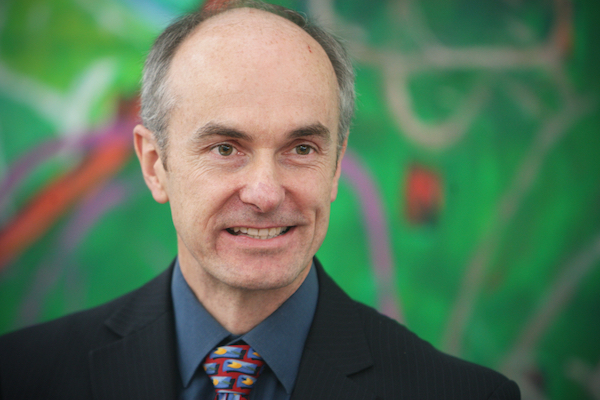
\includegraphics[width=2.3in]{David_MacKay}
\column{0.5\textwidth}
\only<2->{
\includegraphics[width=2.0in]{Mackaybook}}
\end{columns}
\end{frame}
%%--------------------------------------------------------------------------------------
%\begin{frame}{Part II}
%\begin{block}{Goal for Part II}
%Show that the following problems have the same structure as the erasure correction, error correction or syndrome source coding problem and show how to use the \alert{peeling decoder} can be used to solve them
%\end{block}
%
%\begin{block}{Problems}
%\begin{itemize}
%%\item Rateless codes
%\item \alert{Uncoordinated multiple access}
%\item \alert{Sparse Fourier transform (SFT) computation}
%\item Sparse Walsh-Hadamard transform computation	
%\item \alert{Compressed sensing}
%\item Data stream computing
%\item Group testing
%\item Compressive phase retrieval
%\item Sparse covariance estimation
%\end{itemize}
%\end{block}
%
%\end{frame}
%-------------------------------------------------------------
\begin{frame}{Binary erasure channel (BEC) and erasure correction}

\begin{figure}[t]
\centering
\scalebox{0.55}{%\documentclass{article}
%
%\usepackage{tikz}
%\usetikzlibrary{arrows,shapes,chains,matrix,positioning,scopes,patterns,calc}
%\usepackage{color}
%
%\usepackage{latexsym}
%\usepackage{amsmath,amssymb,amsthm}
%\usepackage{etoolbox}
%
%\begin{document}

\begin{tikzpicture}
\def \recW{1in}; %Encoder Length
\def \recH{0.5in}; %Encoder Width

\def \R{0.06in}; %Larger circle radius

\def \Gblks{0.25in}; %Gaps between blocks
\def \ext{0.95in}; %Extensions towards left and right of the figure
\def \extB{0.25in}; %Extensions towards top of the figure

\def \fsizes{\normalsize}; %Defining a generic font size to be adjusted depending on the scaling
\def \fsize{\Large}; %Defining a generic font size to be adjusted depending on the scaling

\tikzstyle{rect}   = [ rectangle, draw, text centered, thick,
                        minimum height=\recH, minimum width=\recW ]

\node [rect](enc) at (0,0) {\fsizes{Encoder}} ;
\node (chan)  [right = \ext of enc,draw,rectangle,text centered,thick,minimum width=1.5in,minimum height=1.5in]{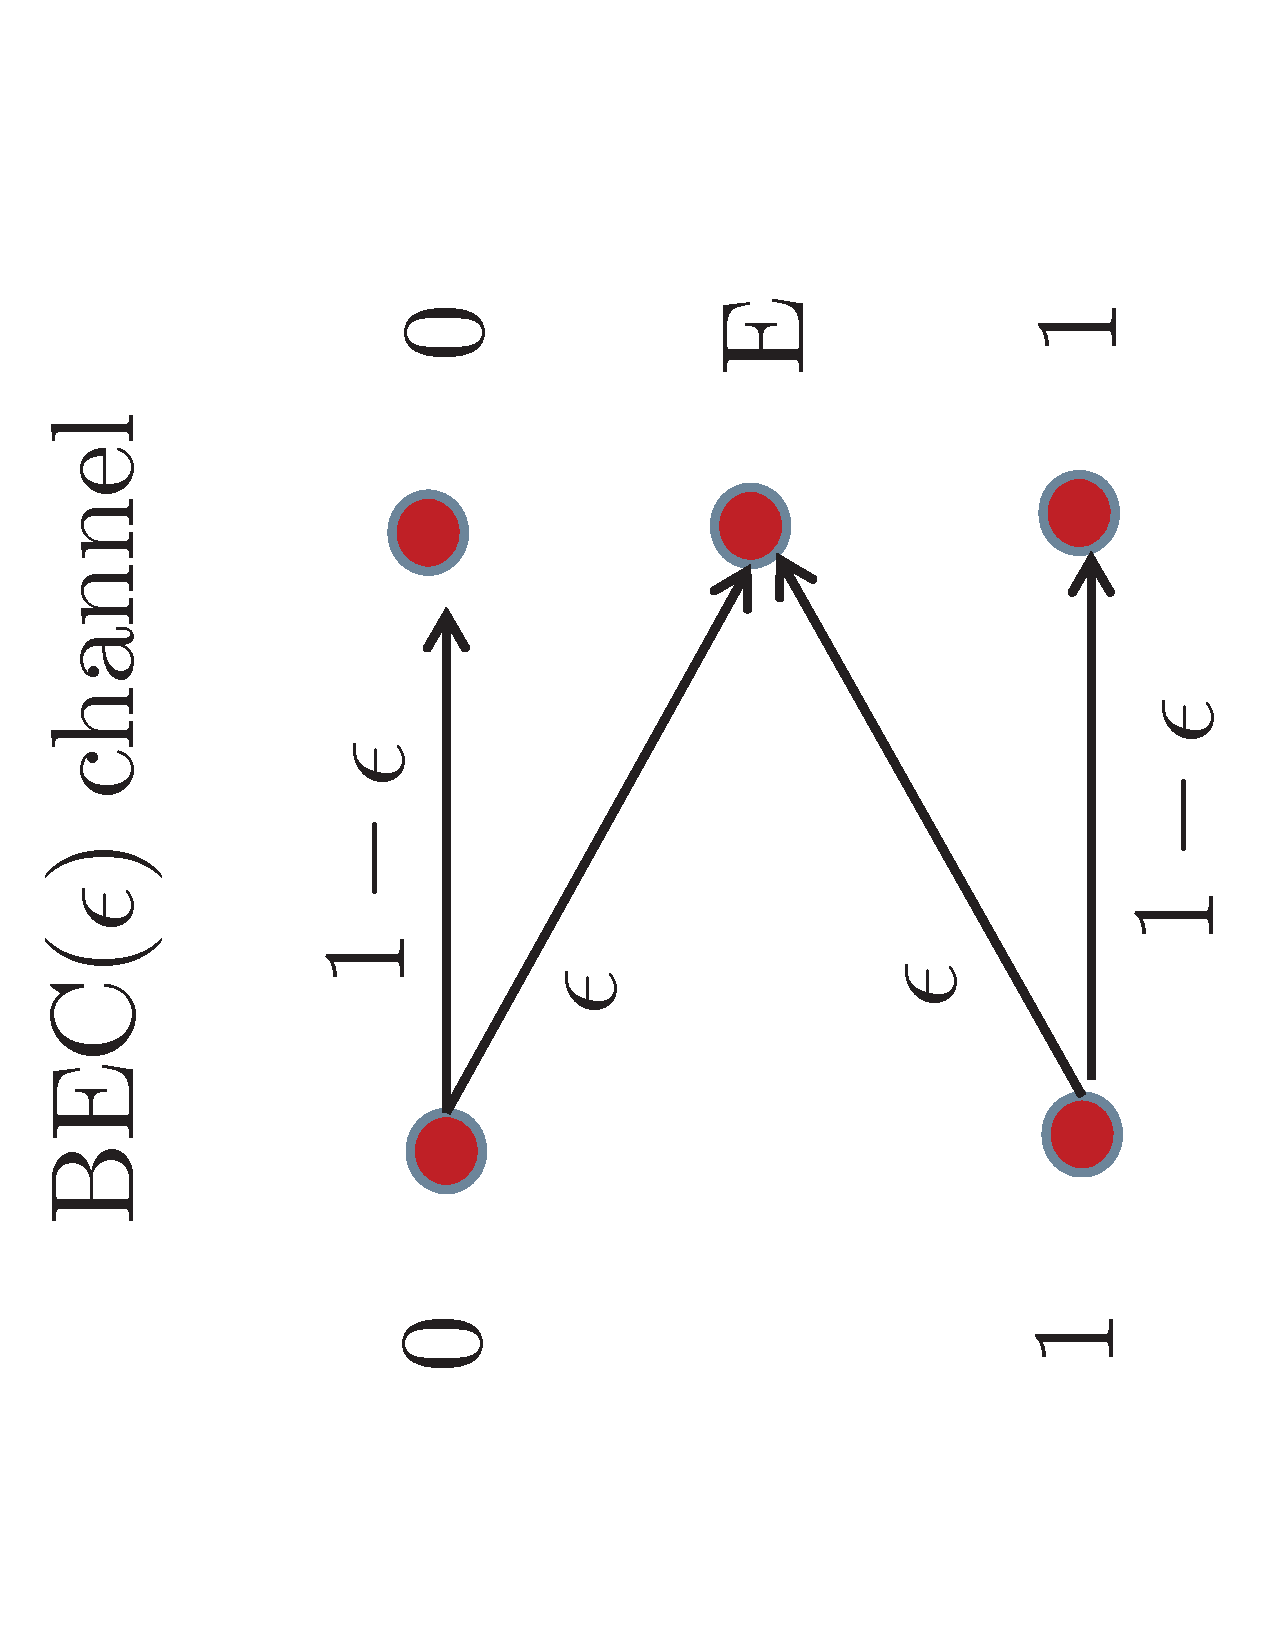
\includegraphics[width=1.5in,angle=-90]{BECchannelmodel.pdf}};
\node (dec)[rect,right=\ext of chan] {\fsizes Decoder} ;

\draw[<-,thick](enc)-- +(-2*\ext,0) node[midway,above]{\fsize $m_1,\ldots,m_k$};
\draw[->,thick](enc)--(chan)node[midway,above]{\fsize $x_1,\ldots,x_n$}node[midway,below]{\fsize $x_i\in \{0,1\}$};
\draw[->,thick](chan)--(dec)node[midway,above]{\fsize $r_1,\ldots,r_n$}node[midway,below]{\fsize $r_i\in \{0,1\}$};;

%\draw[<-,thick](chan)--+(0,\extB) node[above] {\fsize $e_1,\ldots,e_n$};
\draw[->,thick](dec)--+(2*\ext,0)node[midway,above]{\fsize  $\hat{m_1},\ldots,\hat{m_k}$};

\end{tikzpicture}
%\end{document} }
\end{figure}

\begin{block}{Channel coding problem}
\begin{itemize}
\item Transmit a message $\underline{m} = [m_1, \ldots, m_k]^T$ through a binary erasure channel
\item Encode the $k$-bit message $\underline{m}$ into a $n$-bit codeword $\underline{x}$
\item Redundancy is measured in terms of rate of the code $R = k/n$
%\item For $p=2$, capacity $C = 1-H_2(\epsilon)$
%\item A sequence of codes $\{\mathcal{C^n}\}$ is capacity achieving if $P_e^n \rightarrow 0$ while the rate $R^n \rightarrow C$
\end{itemize}
\end{block}

\end{frame}

%--------------------------------------------------------------------------------------
\begin{frame}{Binary erasure channel (BEC) and erasure correction}
%\begin{figure}[t]
%\centering
%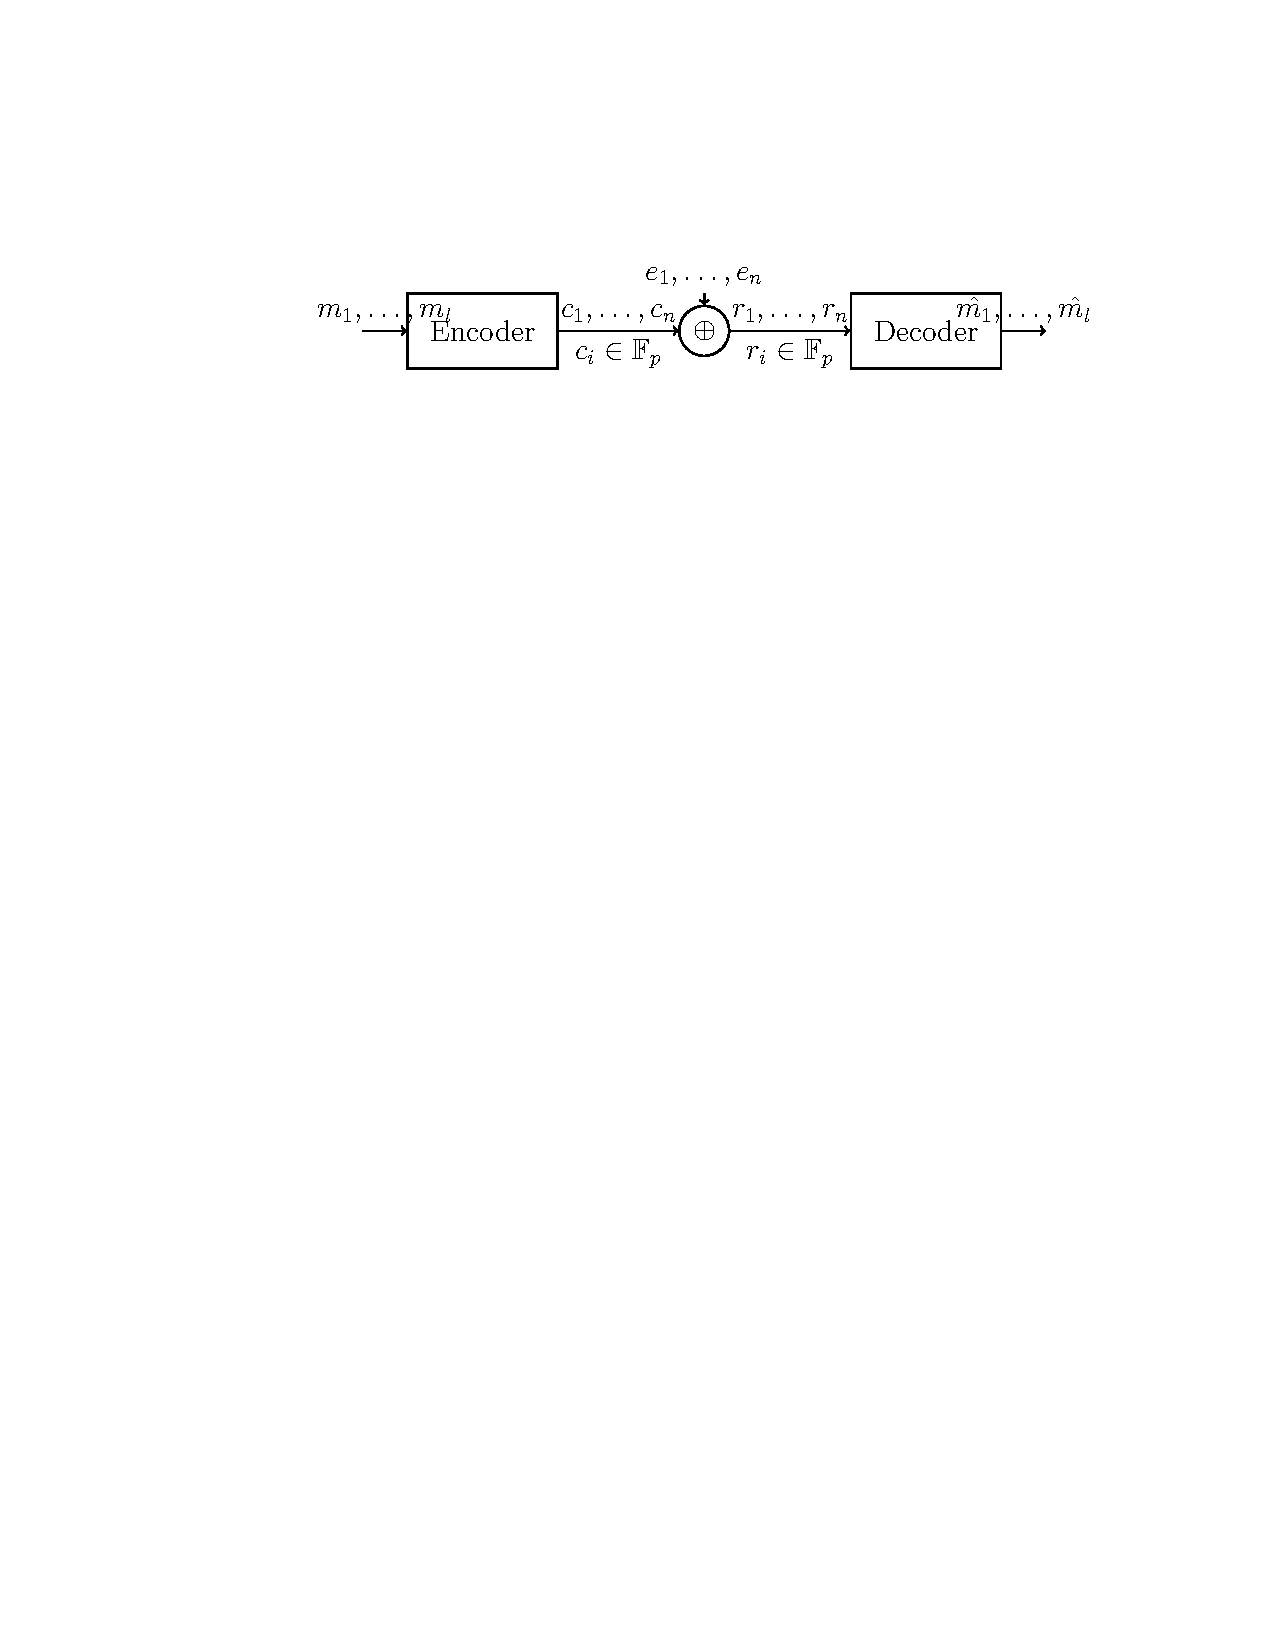
\includegraphics[width=3.0in]{ParySystemModel}
%\end{figure}
%\vspace*{-5mm}
%\begin{figure}[t]
%\centering
%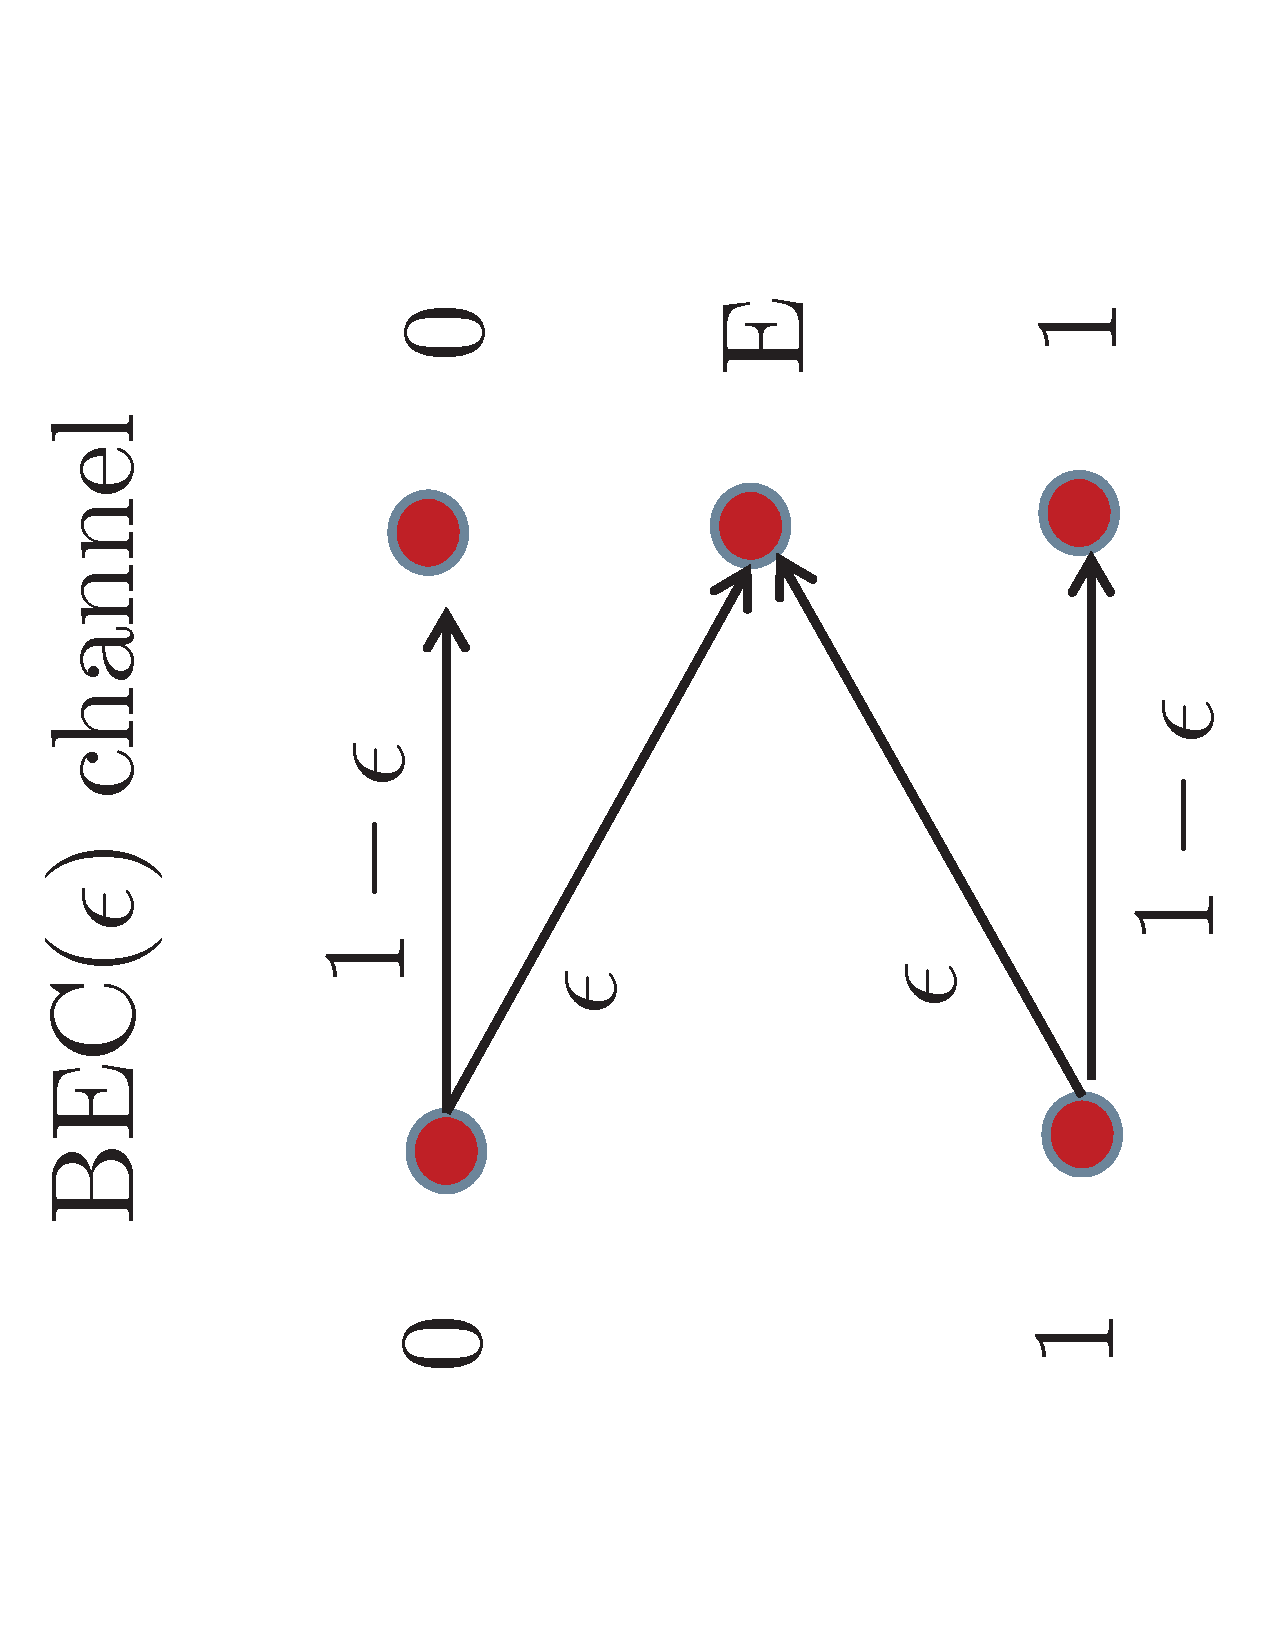
\includegraphics[width=1.0in,angle=-90]{BECchannelmodel}
%\end{figure}
\vspace*{-3mm}
\begin{figure}[t]
\centering
\scalebox{0.55}{%\documentclass{article}
%
%\usepackage{tikz}
%\usetikzlibrary{arrows,shapes,chains,matrix,positioning,scopes,patterns,calc}
%\usepackage{color}
%
%\usepackage{latexsym}
%\usepackage{amsmath,amssymb,amsthm}
%\usepackage{etoolbox}
%
%\begin{document}

\begin{tikzpicture}
\def \recW{1in}; %Encoder Length
\def \recH{0.5in}; %Encoder Width

\def \R{0.06in}; %Larger circle radius

\def \Gblks{0.25in}; %Gaps between blocks
\def \ext{0.95in}; %Extensions towards left and right of the figure
\def \extB{0.25in}; %Extensions towards top of the figure

\def \fsizes{\normalsize}; %Defining a generic font size to be adjusted depending on the scaling
\def \fsize{\Large}; %Defining a generic font size to be adjusted depending on the scaling

\tikzstyle{rect}   = [ rectangle, draw, text centered, thick,
                        minimum height=\recH, minimum width=\recW ]

\node [rect](enc) at (0,0) {\fsizes{Encoder}} ;
\node (chan)  [right = \ext of enc,draw,rectangle,text centered,thick,minimum width=1.5in,minimum height=1.5in]{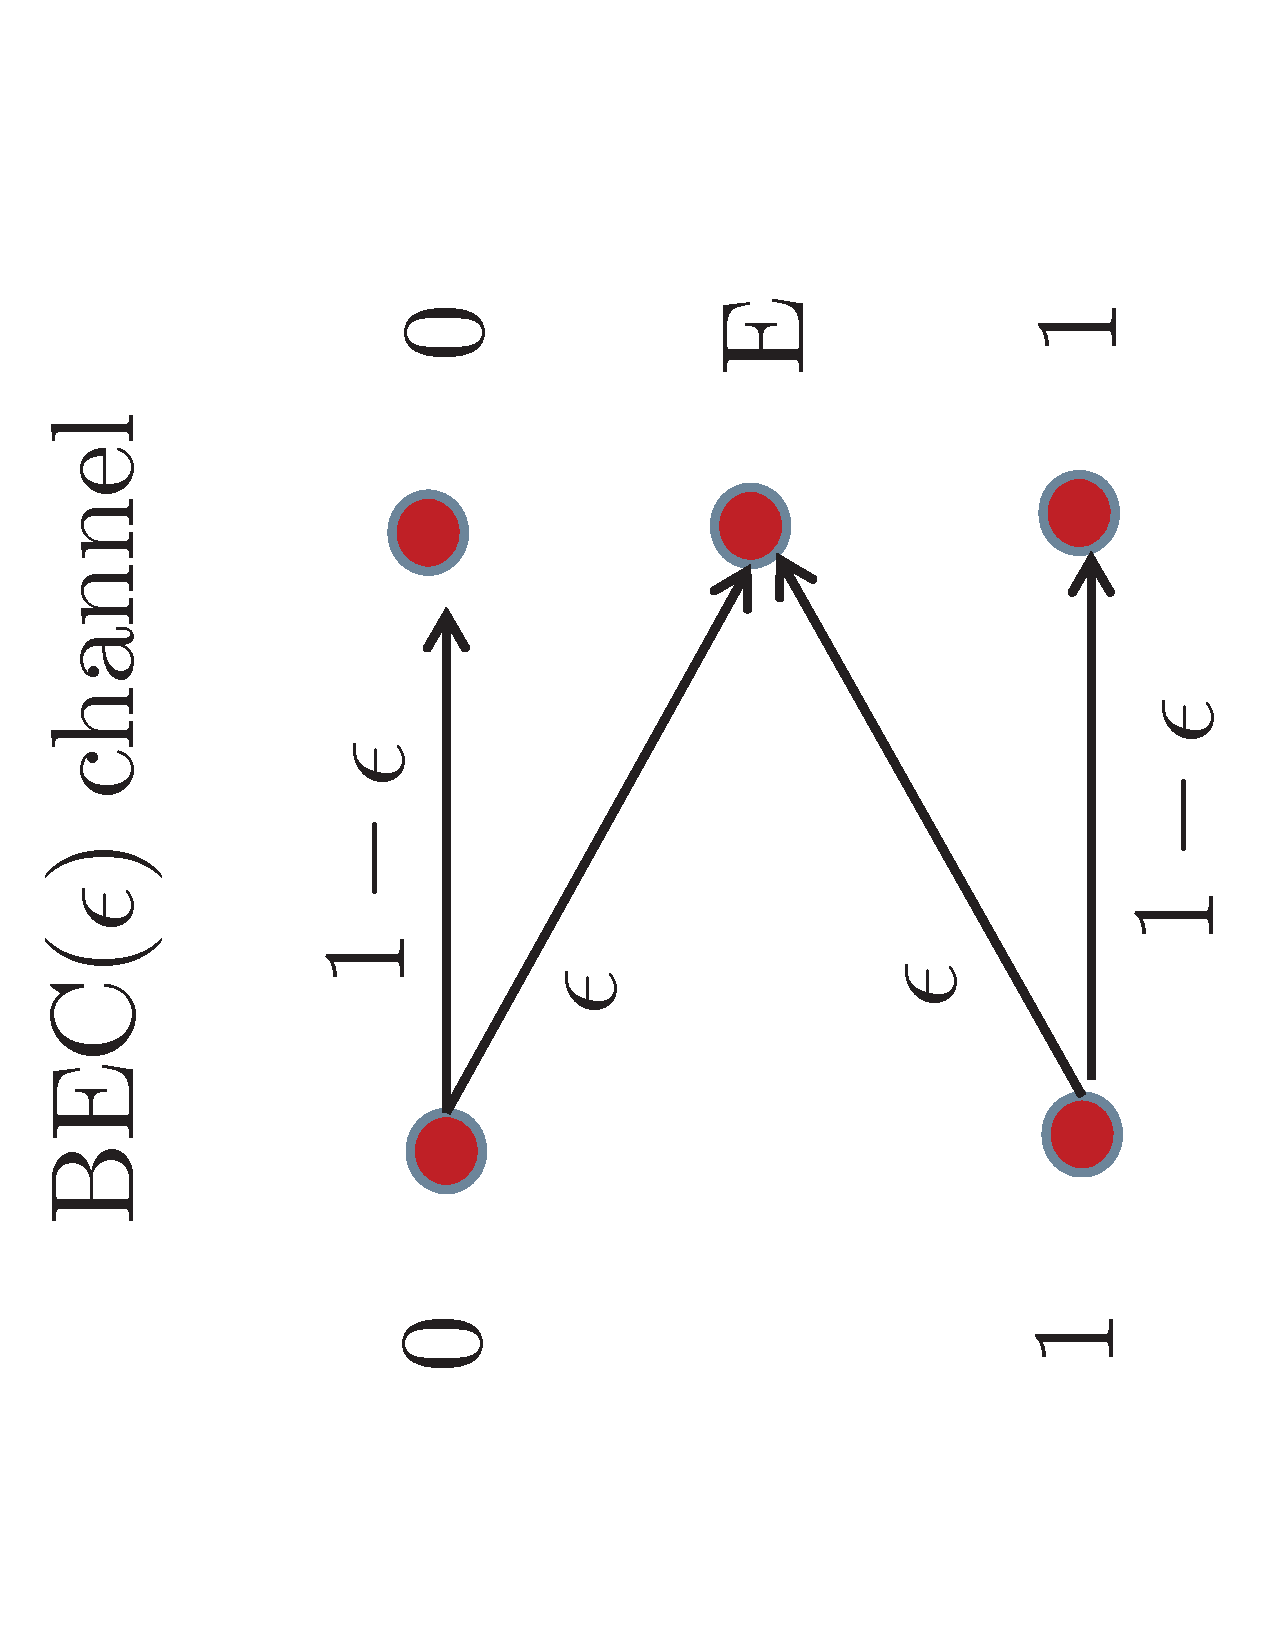
\includegraphics[width=1.5in,angle=-90]{BECchannelmodel.pdf}};
\node (dec)[rect,right=\ext of chan] {\fsizes Decoder} ;

\draw[<-,thick](enc)-- +(-2*\ext,0) node[midway,above]{\fsize $m_1,\ldots,m_k$};
\draw[->,thick](enc)--(chan)node[midway,above]{\fsize $x_1,\ldots,x_n$}node[midway,below]{\fsize $x_i\in \{0,1\}$};
\draw[->,thick](chan)--(dec)node[midway,above]{\fsize $r_1,\ldots,r_n$}node[midway,below]{\fsize $r_i\in \{0,1\}$};;

%\draw[<-,thick](chan)--+(0,\extB) node[above] {\fsize $e_1,\ldots,e_n$};
\draw[->,thick](dec)--+(2*\ext,0)node[midway,above]{\fsize  $\hat{m_1},\ldots,\hat{m_k}$};

\end{tikzpicture}
%\end{document} }
\end{figure}
\vspace*{-3mm}
\begin{block}{Capacity achieving sequence of codes}
\begin{itemize}
\pause \item Capacity $C(\epsilon) = 1-\epsilon$
\pause  \item A sequence of codes $\{\mathcal{C}^n\}$
  \item Probability of erasure $P_e^n$
  \item Rate $R^n$
  \item Capacity achieving if $P_e^n \rightarrow 0$ as $n \rightarrow \infty$ while $R^n \rightarrow C$
\pause  \item \alert{Find efficient encoders/decoders in terms encoding and decoding complexities}
\end{itemize}
\end{block}
\pause
\begin{block}{Significance of the erasure channel}
\begin{itemize}
  \item Introduced by Elias in 1954 as a toy example
%  \item Good model for transmission of packets over the Internet
  \item Has become the canonical model for coding theorists to gain insight
\end{itemize}
\end{block}


\end{frame}



%%-----------------------------------------------------		
%\begin{frame}{$(n,k)$ Binary linear block codes - basics}
%\begin{block}{Generator matrix - $\mathbf{G}$ is a $n \times k$ encoding matrix}	
%\[
%\begin{bmatrix}
%  g_{1,1} & \cdots & g_{k,l} \\
%  \vdots & \ddots & \vdots \\
%  \vdots & \ddots & \vdots \\
%  g_{n,1} &  & g_{k,l} \\
%\end{bmatrix}
%\begin{bmatrix}
%  m_1 \\
%  \vdots \\
%  m_k \\
%\end{bmatrix}
%=
%\begin{bmatrix}
%  x_1 \\
%  \vdots \\
%  \vdots \\
%  x_n \\
%\end{bmatrix}
%\pause
%\bigoplus
%\begin{bmatrix}
%  e_1 \\
%  \vdots \\
%  \vdots \\
%  e_n \\
%\end{bmatrix}
%=
%\begin{bmatrix}
%  r_1 \\
%  \vdots \\
%  \vdots \\
%  r_n \\
%\end{bmatrix}
%\]
%%\[ \mathbf{G}_{n \times k} \underline{m}_{k \times 1} = \underline{c}_{n \times 1} \oplus \underline{e}_{n \times 1} = \underline{r}_{n \times 1} \]
%\pause
%\begin{eqnarray}
%\nonumber \underline{x} & = & \mathbf{G} \underline{m} \\
%\nonumber \underline{r} & = & \underline{x} \oplus \underline{e}
%\end{eqnarray}
%\end{block}
%\pause
%\begin{block}{Parity check matrix - $\mathbf{H}$ is a $(n-k) \times n$ matrix such that $\mathbf{H} \mathbf{G} = \mathbf{0}$}
%\[
%\underline{y} = \mathbf{H} \underline{r} = \mathbf{H} \underline{x} \oplus \mathbf{H} \underline{e} = \underline{0} \oplus \mathbf{H} \underline{e}
%\]
%\end{block}
%\end{frame}

%-----------------------------------------------------		
\begin{frame}{$(n,k)$ Binary linear block codes - basics}
\begin{columns}[t]
\column{0.47\textwidth}
\begin{block}{$\mathbf{G}$ is a $n \times k$ generator matrix}	
\[
\begin{bmatrix}
  g_{1,1} & \cdots & g_{k,l} \\
  \vdots & \ddots & \vdots \\
  \vdots & \ddots & \vdots \\
  g_{n,1} &  & g_{k,l} \\
\end{bmatrix}
\begin{bmatrix}
  m_1 \\
  \vdots \\
  m_k \\
\end{bmatrix}
=
\begin{bmatrix}
  x_1 \\
  \vdots \\
  \vdots \\
  x_n \\
\end{bmatrix}
\]
\end{block}

\column{0.5\textwidth}
\begin{block}{Example - (6,3) code}
\[
\ \
\begin{bmatrix}
  1 & 0 & 0 \\
  0 & 1 & 0 \\
  0 & 0 & 1 \\
  1 & 0 & 1 \\
  1 & 1 & 0 \\
  0 & 1 & 1 \\
\end{bmatrix}
\begin{bmatrix}
  1 \\
  1 \\
  0 \\
\end{bmatrix}
=
\begin{bmatrix}
1\\
1\\
0\\
1\\
0\\
1\\
\end{bmatrix}
\]
\end{block}
\end{columns}
\pause
\begin{block}{Parity check matrix - $\mathbf{H}$ is a $(n-k) \times n$ matrix s.t. $\Hm \Gm = \mathbf{0} \Rightarrow \Hm \xv = 0$}
\[
\Hm = \begin{bmatrix}
  1 & 0 & 1 & 1 & 0 & 0 \\
  1 & 1 & 0 & 0 & 1 & 0 \\
  0 & 0 & 1 & 0 & 0 & 1 \\
\end{bmatrix}
\begin{bmatrix}
1\\
1\\
0\\
1\\
0\\
1\\
\end{bmatrix}
=
\begin{bmatrix}
0\\
0\\
0\\
\end{bmatrix}
\]
\end{block}
\end{frame}

%%--------------------------------------------------------------------------------------
%\begin{frame}{Brief survey of the literature}
%\begin{itemize}
%\item The binary erasure channel (BEC) introduced by Elias in 1954
%\pause
%\item Regular LDPC codes introduced by Gallager in 1962, 1963
%\pause
%\item Zyablov and Pinsker considered peeling decoder in 1974
%\pause
%\item Papers by Luby, Mitzenmacher, Shokrollahi, Spielman, Stemann 1997-2001
%\pause
%\item Rateless codes introduced by Luby in 2002
%\pause
%\item EXIT chart analysis by ten Brink'99 and Ashikmin, Kramer and ten Brink'04
%\pause
%\item Summarized in Modern coding theory book by Richardson and Urbanke
%\end{itemize}
%\end{frame}
%--------------------------------------------------------------------------------------
\begin{frame}{Tanner graph representation of codes}
\begin{columns}
\column{0.5\textwidth}
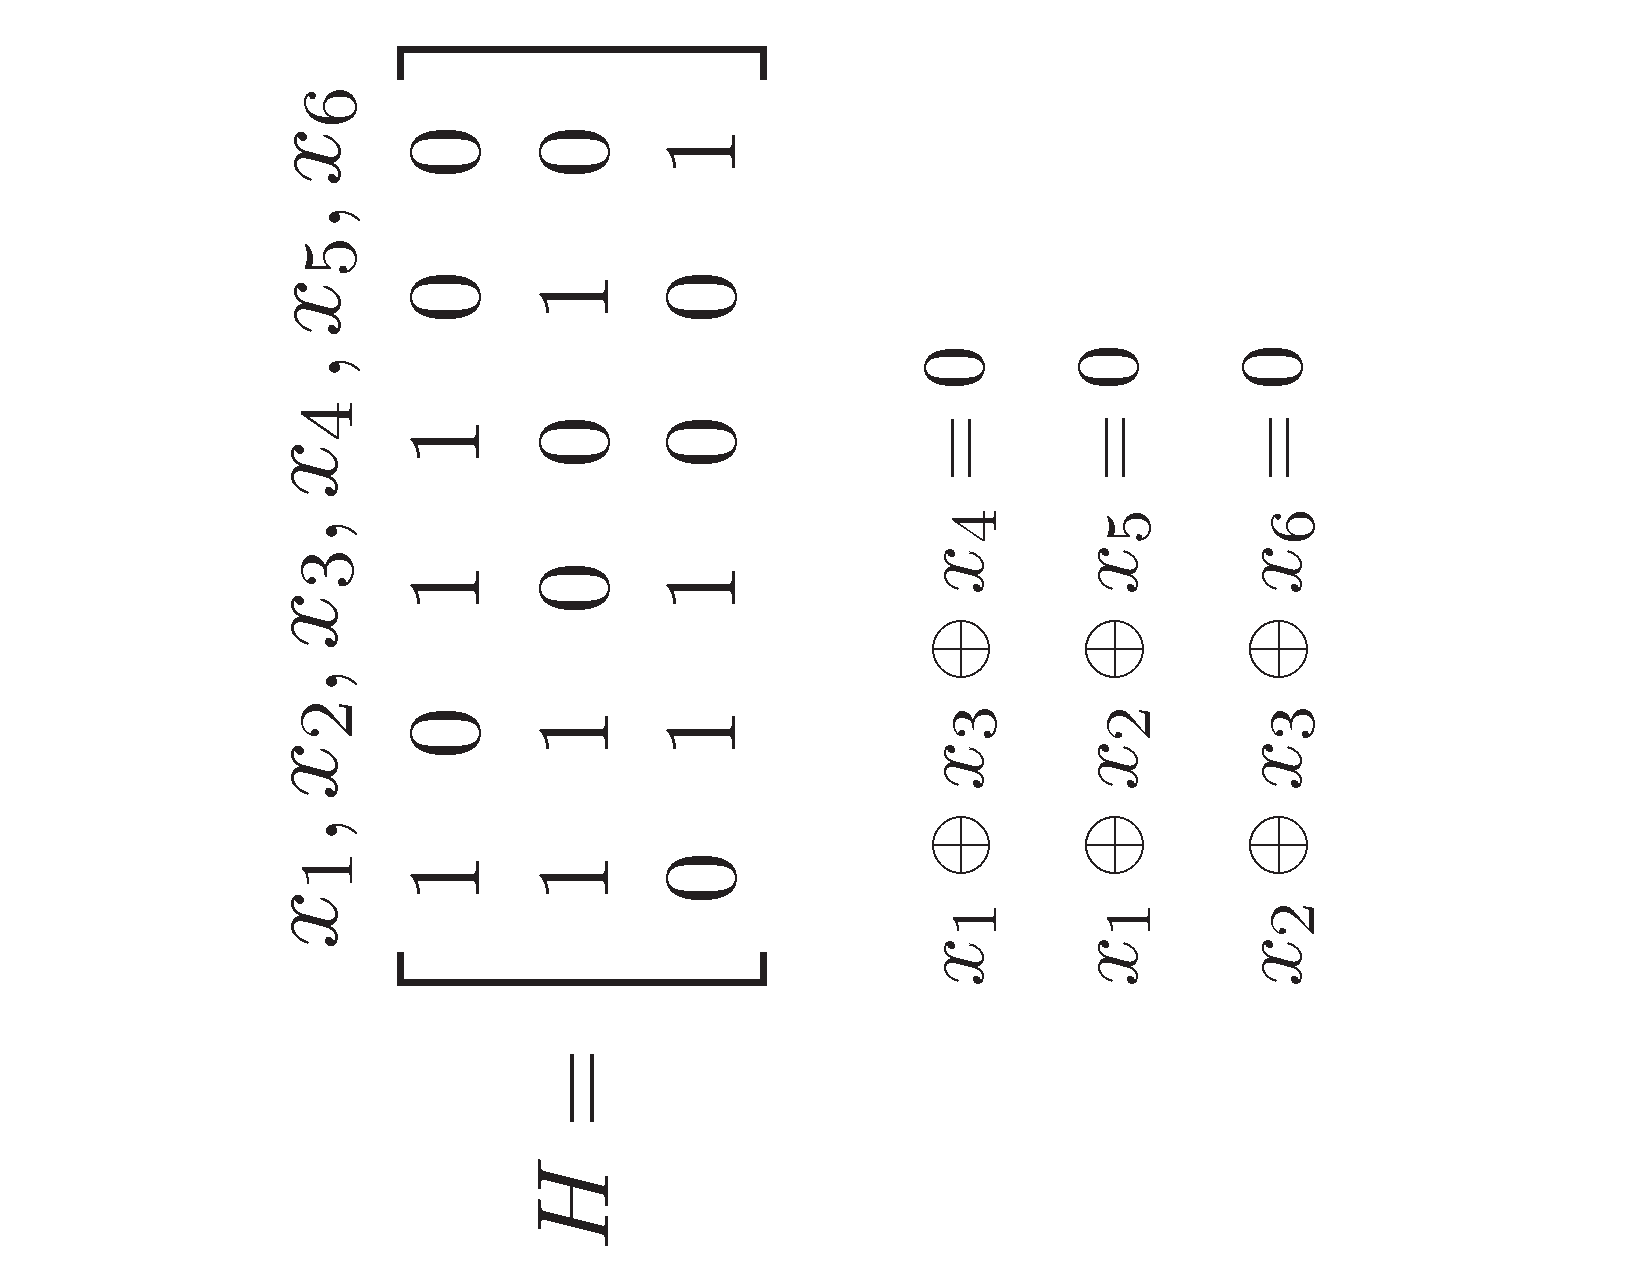
\includegraphics[width=2.3in,angle=-90]{paritycheckmatrix63code}
\column{0.5\textwidth}
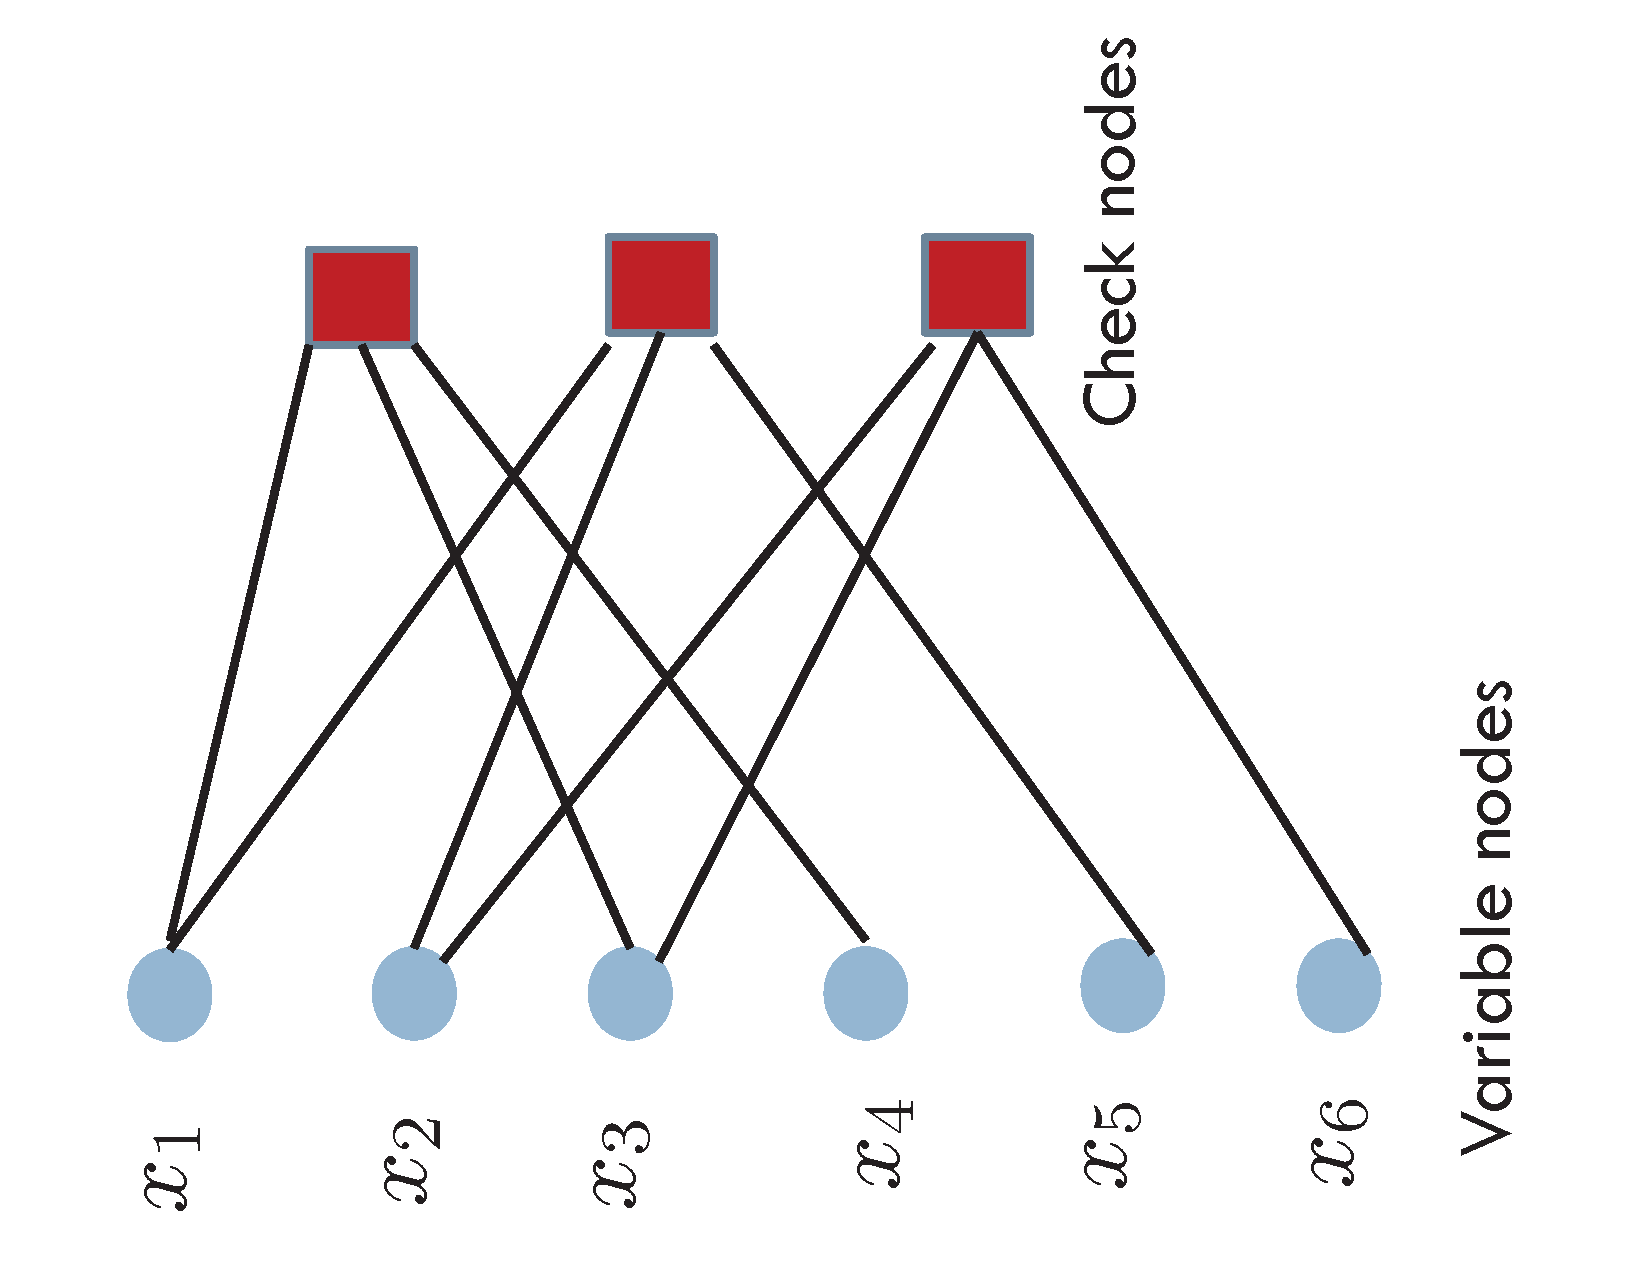
\includegraphics[width=2.25in,angle=-90]{Tannergraph63code}
\end{columns}
\begin{block}{}
\begin{itemize}
    \item Gallager'63, Tanner'81
    \item Parity check matrix implies that $\Hm \xv = 0$
    \item Code constraints can be specified in terms of a bipartite (Tanner) graph
  %\item A code can be specified by giving the Tanner graph
\end{itemize}
\end{block}
\end{frame}
%--------------------------------------------------------------------------------------
\begin{frame}{Peeling decoder for the BEC}
\vspace{-5mm}
\begin{columns}
\column{0.5\textwidth}
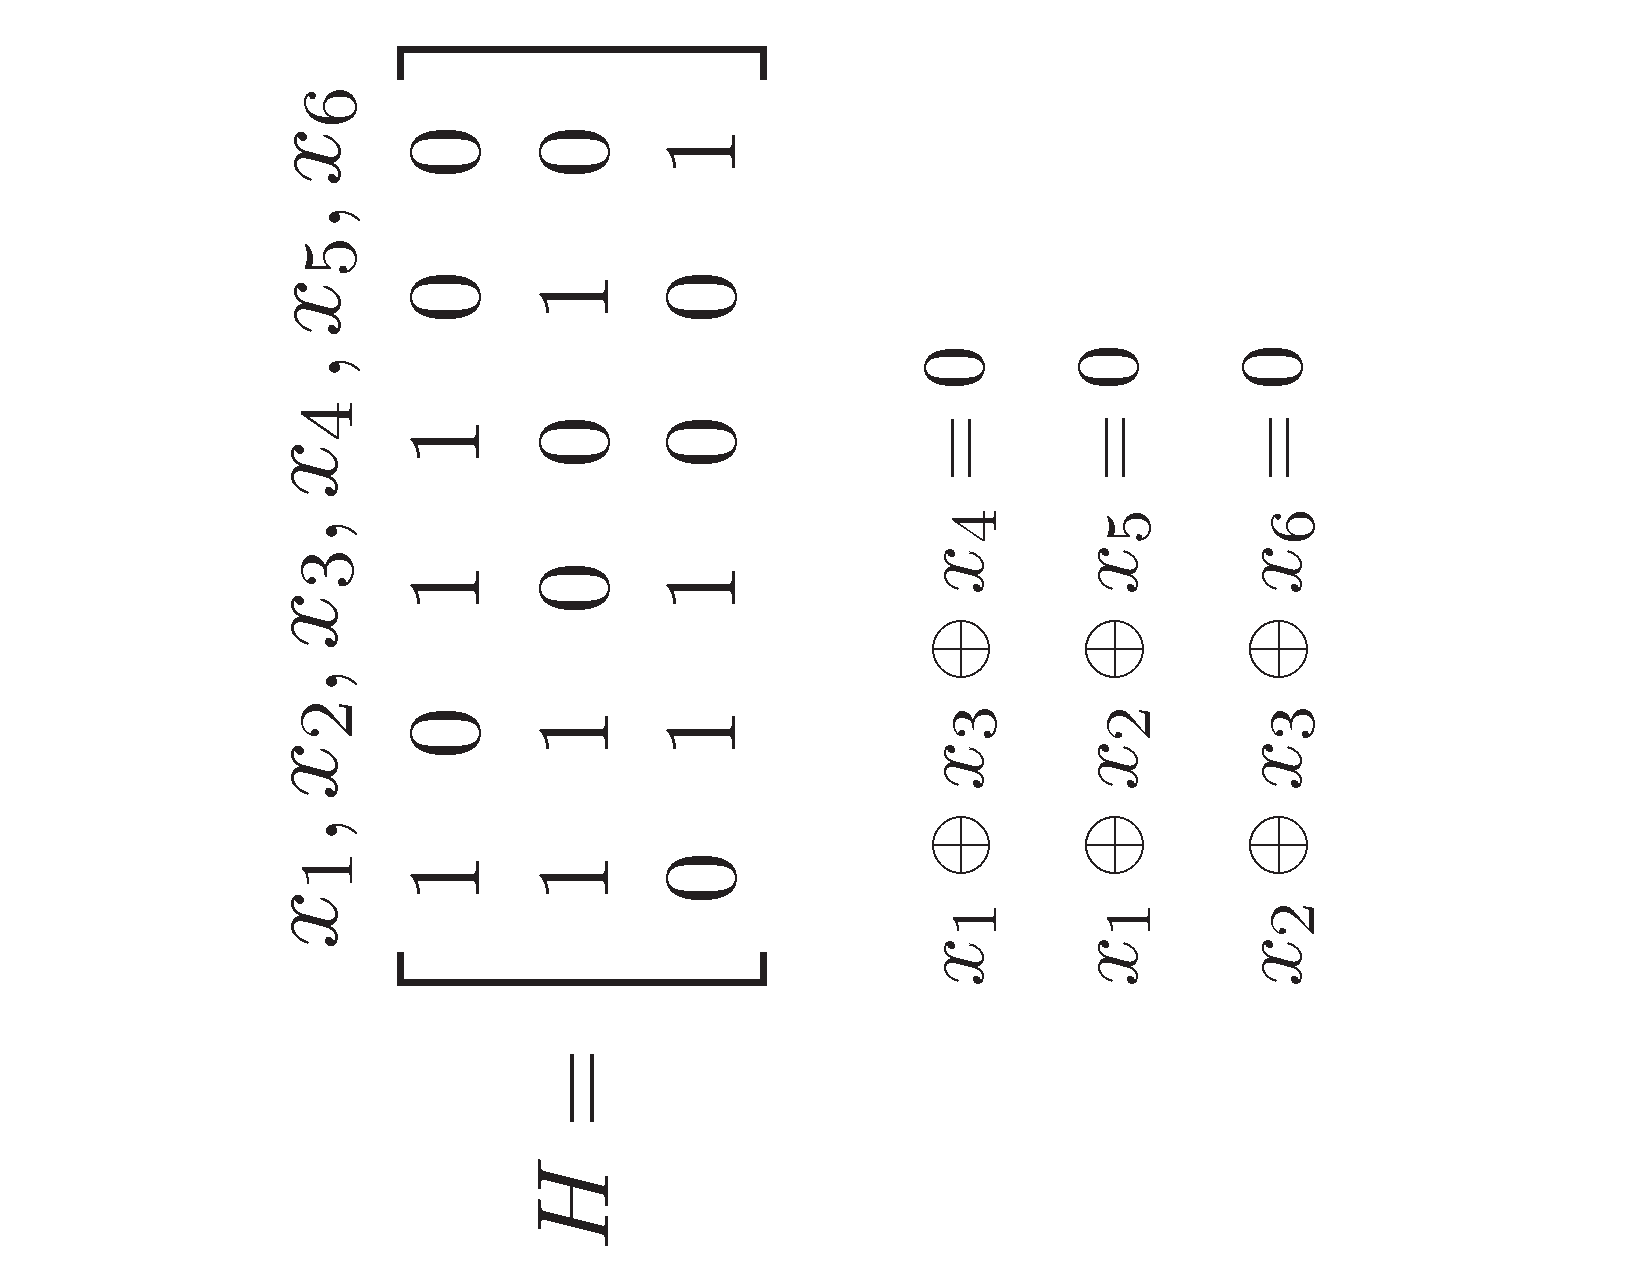
\includegraphics[width=2.3in,angle=-90]{paritycheckmatrix63code}
\column{0.5\textwidth}
%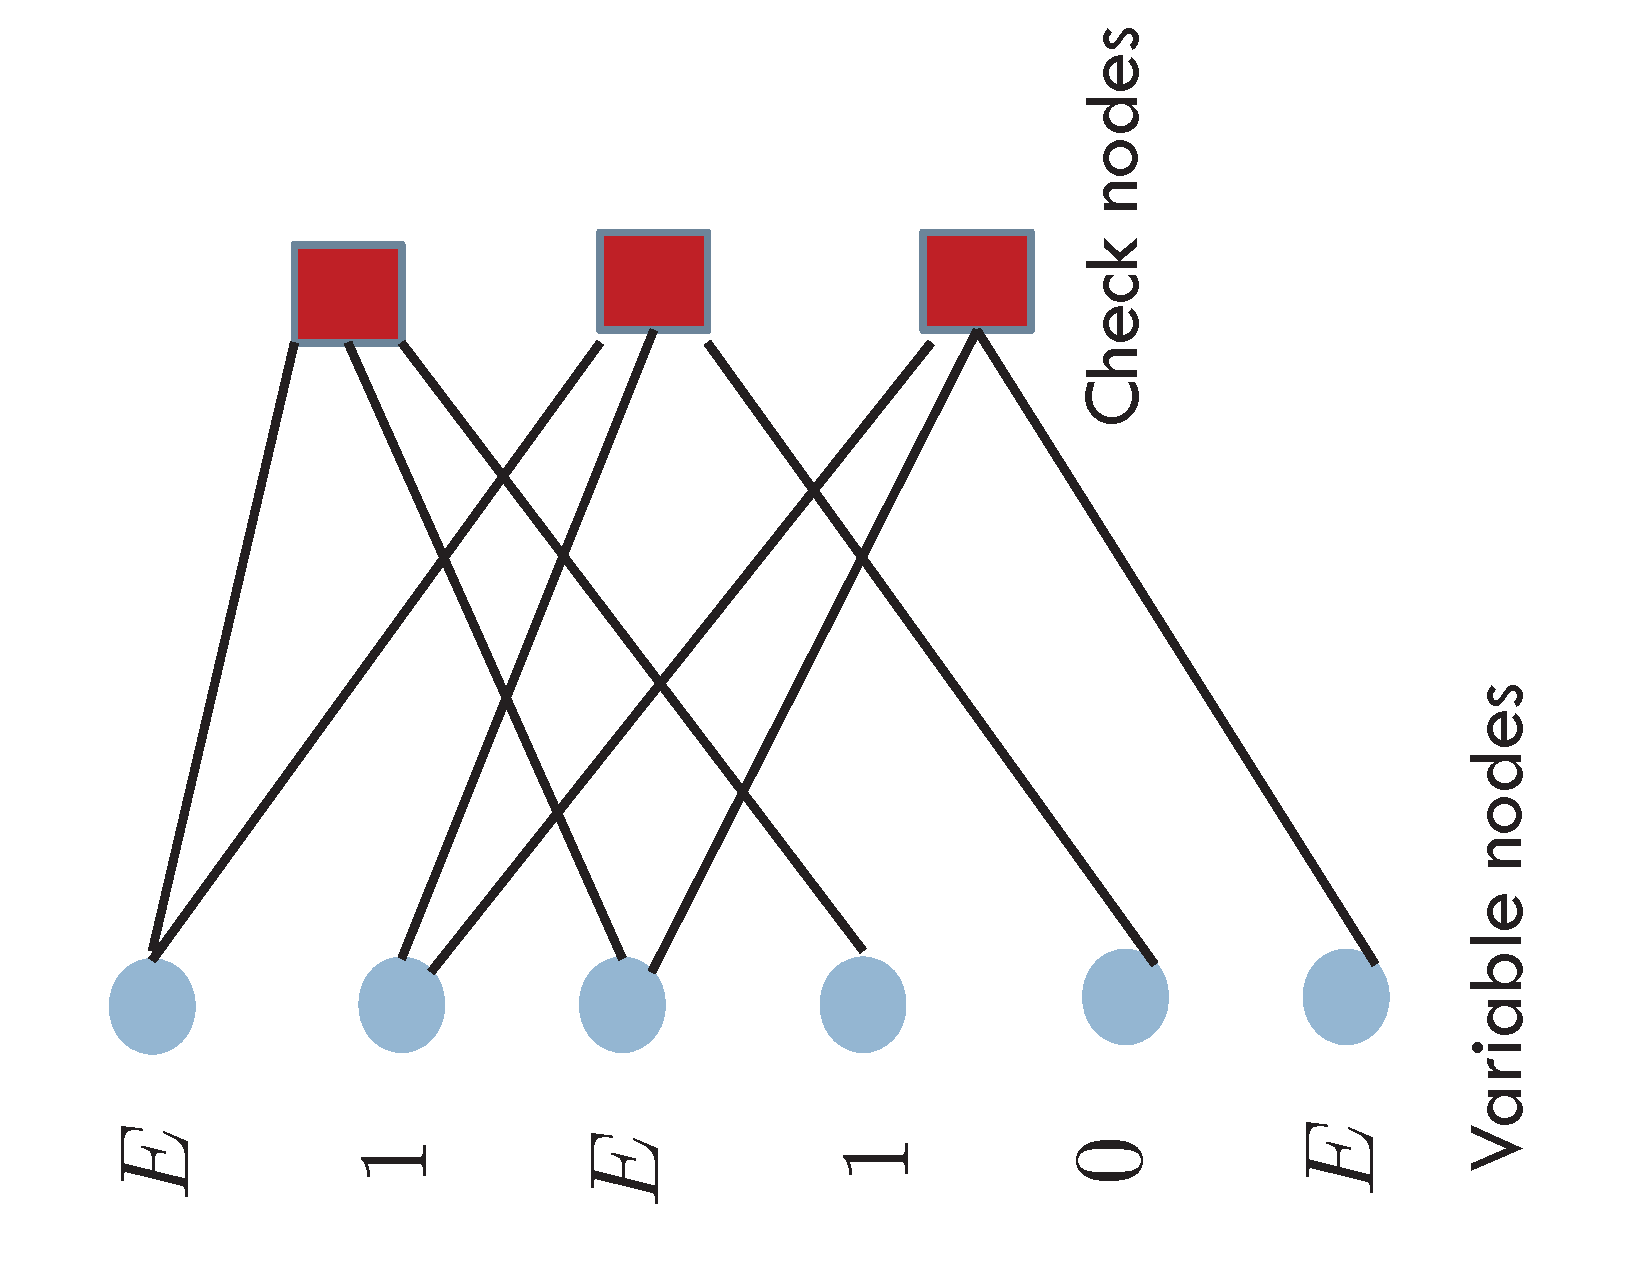
\includegraphics[width=2.25in,angle=-90]{Tannergraph63codewitherasures}
\scalebox{1}{\pgfdeclarelayer{background}
\pgfdeclarelayer{foreground}
\pgfdeclarelayer{m-f}
\pgfdeclarelayer{main}

\pgfsetlayers{background,foreground}
\colorlet{LightBlue}{blue!10!white}
\colorlet{DarkBlue}{blue!80!white}

\begin{tikzpicture}[scale=1.0]
\clip (-0.15in,0.15in) rectangle (1.3in,-2.5in);

\def\n     {6}   % #-Variable nodes
\def\m     {3}  % #-Check nodes
\def\nodewidth{0.15in}
\def\nodegapVN{0.3in}
\def\nodegapCN{0.5in}

\tikzstyle{check} = [rectangle, draw, text centered, thick, fill=red,
                          minimum height=\nodewidth, minimum width=\nodewidth]
\tikzstyle{bit} = [circle, draw, text centered, thick, fill=LightBlue,
                          radius=0.5*\nodewidth]
\tikzstyle{bitpeeled} = [circle, draw, text centered, thick, fill=DarkBlue,
                          radius=0.5*\nodewidth]

\begin{pgfonlayer}{background}
%\draw[gray,step=0.5in] (-0.15in,0.15in) grid (1.5in,-2.5in);
\foreach \vn in {1,...,\n}{
  \node[bit] (vn\vn) at (0,-\vn*\nodegapVN) {};
 }

 \foreach \cn in {1,...,\m}{
  \node[check] (cn\cn) at (1in,-\cn*\nodegapCN) {};
 }
\end{pgfonlayer}



\begin{pgfonlayer}{foreground}

%Text to left of VN
\only<1>{
\foreach \vn in {1,...,\n}{
  \node[left] (nodetxt) at (vn\vn.west) {\normalsize{$x_\vn$}};
 	}  	
}

\only<2-8>{
\foreach \vn/\txt in {2/1,4/1,5/0}{
\node[left] (nodetxt) at (vn\vn.west) {\normalsize{\txt}};
 	}	
}

\only<2-3>\node[left] (nodetxt) at (vn1.west) {\normalsize{E}};
\only<2-5>\node[left] (nodetxt) at (vn3.west) {\normalsize{E}};
\only<2-7>\node[left] (nodetxt) at (vn6.west) {\normalsize{E}};


\only<4-8>\node[left] (nodetxt) at (vn1.west) {\normalsize{E=1}};
\only<6-8>\node[left] (nodetxt) at (vn3.west) {\normalsize{E=0}};
\only<8>\node[left] (nodetxt) at (vn6.west) {\normalsize{E=1}};

%Edges
\uncover<1-2>{
\foreach \vn/\cn in {2/2,2/3,4/1,5/2}{
 \draw[thick] (vn\vn.east)--(cn\cn.west);
  }
}

\only<1-3>\draw[thick] (vn1.east)--(cn2.west);
\only<1-4>\draw[thick] (vn1.east)--(cn1.west);

\only<1-5>\draw[thick] (vn3.east)--(cn1.west);
\only<1-6>\draw[thick] (vn3.east)--(cn3.west);

\only<1-5>\draw[thick] (vn3.east)--(cn1.west);
\only<1-6>\draw[thick] (vn3.east)--(cn3.west);

\only<1-7> \draw[thick] (vn6.east)--(cn3.west);

%% Peeled bits color
\uncover<3-8>{
  \foreach \vn in {2,4,5}{
    \node[bitpeeled] () at (vn\vn) {};
    }
  }
 \only<4-8>\node[bitpeeled] () at (vn1) {};
 \only<6-8>\node[bitpeeled] () at (vn3) {};
  \only<8>\node[bitpeeled] () at (vn6) {};

%Check node values
\only<2,5,6,7,8> \node[right] (nodetxt) at (cn1.east) {\normalsize{0}};
\only<3,4> \node[right] (nodetxt) at (cn1.east) {\normalsize{1}};

\only<2,4,5,6,7,8> \node[right] (nodetxt) at (cn2.east) {\normalsize{0}};
\only<3> \node[right] (nodetxt) at (cn2.east) {\normalsize{1}};

\only<2,6,7,8> \node[right] (nodetxt) at (cn3.east) {\normalsize{0}};
\only<3,4,5> \node[right] (nodetxt) at (cn3.east) {\normalsize{1}};



%% Text at the bottom
\only<1> \node[minimum width=10cm] (txt) at (0.5in,-7*\nodegapVN) {Tanner Graph};
\only<2> \node[minimum width=10cm] (txt) at (0.5in,-7*\nodegapVN) {Received block};
\only<3> \node[minimum width=10cm] (txt) at (0.5in,-7*\nodegapVN) {Peeling Step 1};
\only<4-5> \node[minimum width=10cm] (txt) at (0.5in,-7*\nodegapVN) {Peeling Step 2};
\only<6-7> \node[minimum width=10cm] (txt) at (0.5in,-7*\nodegapVN) {Peeling Step 3};
\only<8> \node[minimum width=10cm] (txt) at (0.5in,-7*\nodegapVN) {Peeling Step 4};

\end{pgfonlayer}
\end{tikzpicture} }
\end{columns}
\begin{block}{}
\begin{itemize}
  \item Zyablov and Pinsker'74, Luby et al '95
  \item Remove edges incident on known variable nodes and adjust check node values
  \item If there is a check node with a \alert{single edge}, it can be recovered
\end{itemize}
\end{block}
\end{frame}
%--------------------------------------------------------------------------------------
\begin{frame}{Message passing decoder for the BEC}
\vspace{-5mm}
\begin{columns}
\column{0.5\textwidth}
%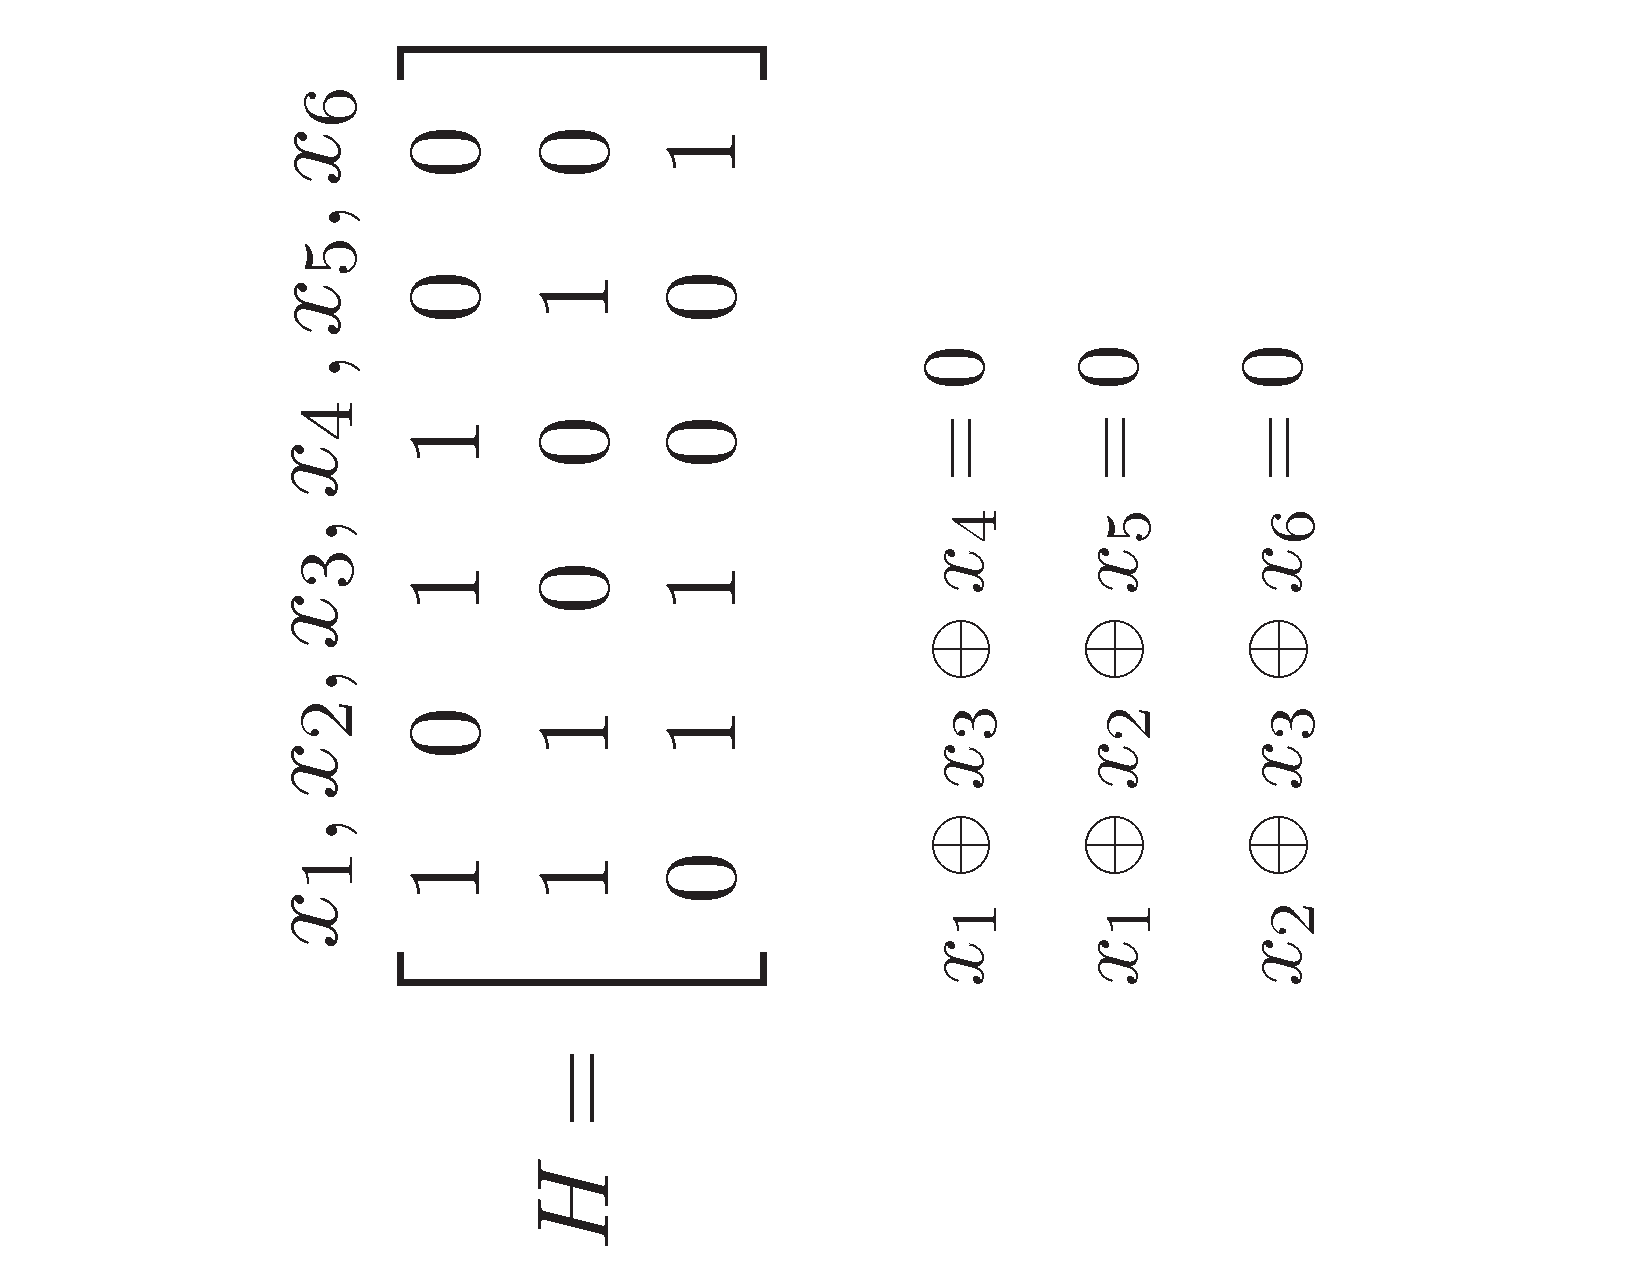
\includegraphics[width=2.3in,angle=-90]{paritycheckmatrix63code}
%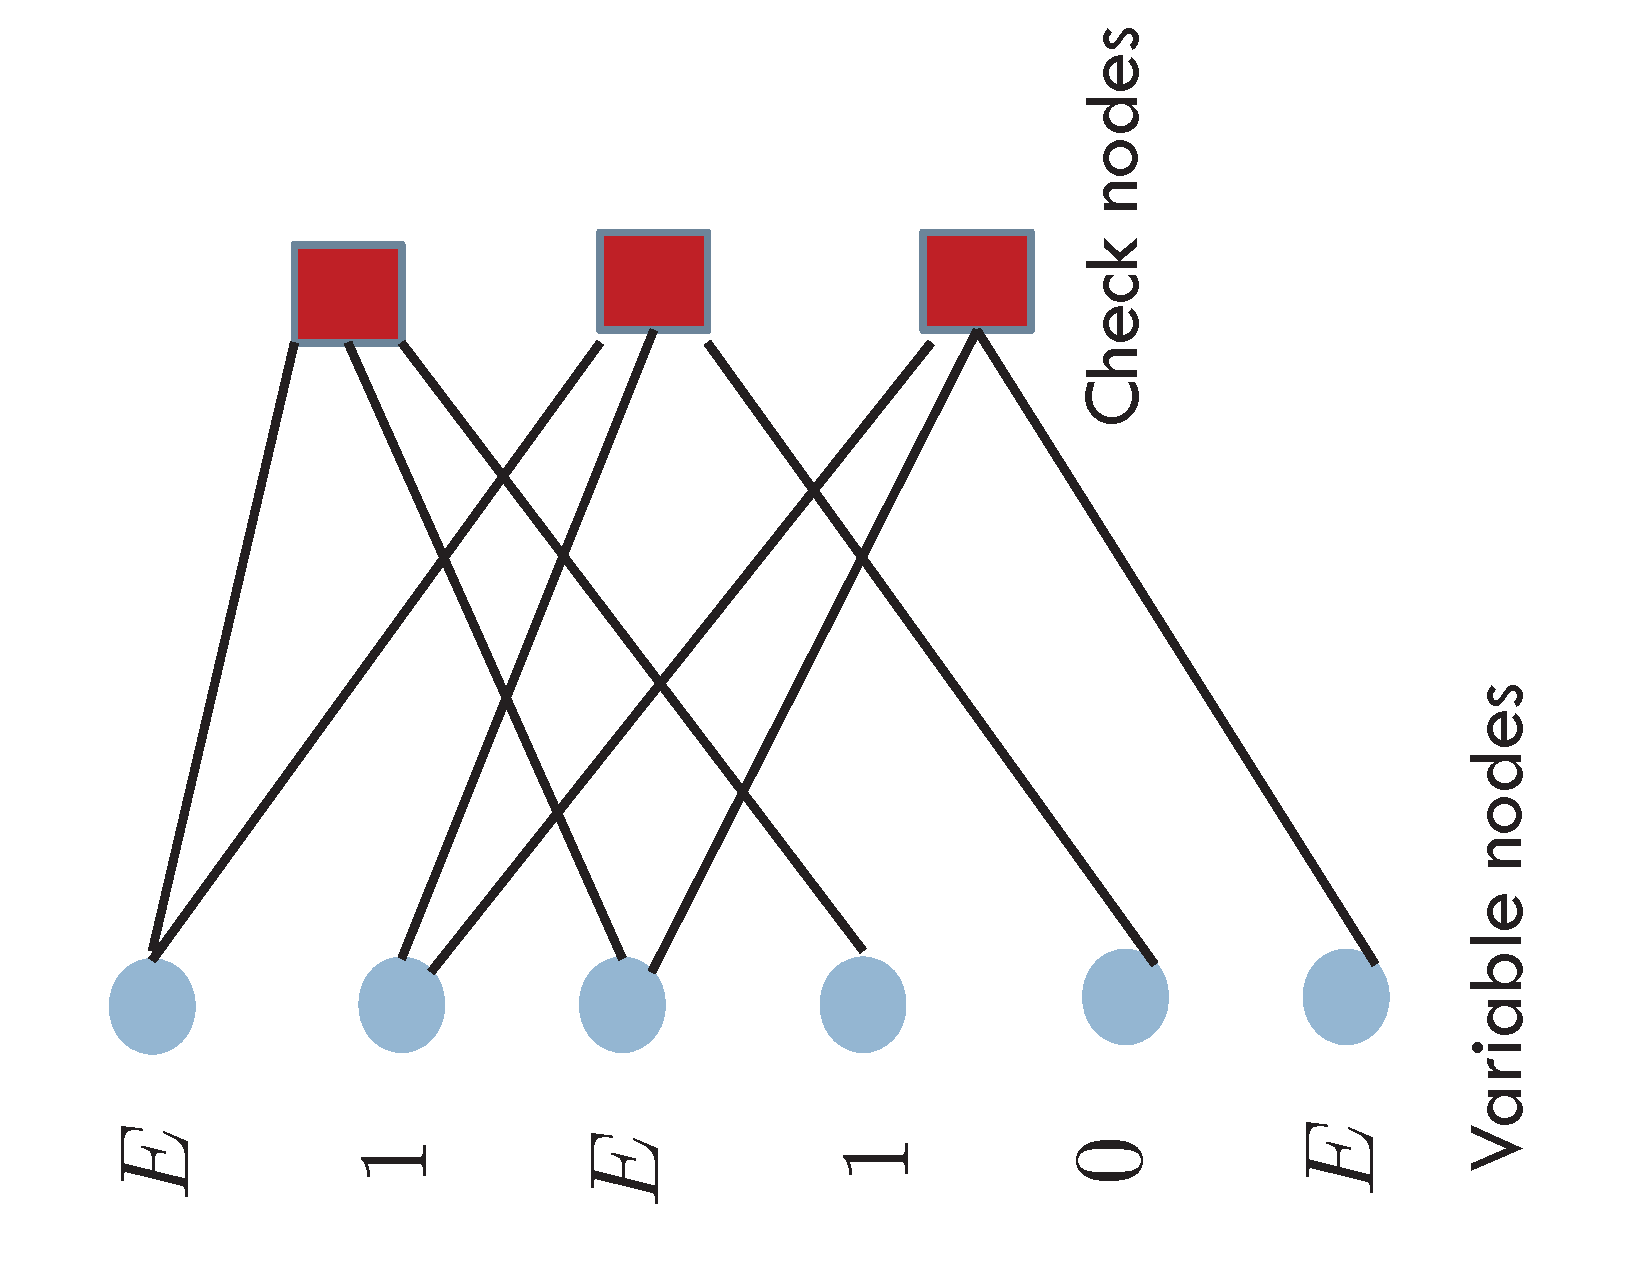
\includegraphics[width=2.25in,angle=-90]{Tannergraph63codewitherasures}
\scalebox{1}{\pgfdeclarelayer{background}
\pgfdeclarelayer{foreground}
\pgfdeclarelayer{m-f}
\pgfdeclarelayer{main}

\pgfsetlayers{background,foreground}
\colorlet{LightBlue}{blue!10!white}
\colorlet{DarkBlue}{blue!80!white}

\begin{tikzpicture}[scale=1.0]
\clip (-0.15in,0.15in) rectangle (1.3in,-2.5in);

\def\n     {6}   % #-Variable nodes
\def\m     {3}  % #-Check nodes
\def\nodewidth{0.15in}
\def\nodegapVN{0.3in}
\def\nodegapCN{0.5in}

\tikzstyle{check} = [rectangle, draw, text centered, thick, fill=red,
                          minimum height=\nodewidth, minimum width=\nodewidth]
\tikzstyle{bit} = [circle, draw, text centered, thick, fill=LightBlue,
                          radius=0.5*\nodewidth]
\tikzstyle{bitpeeled} = [circle, draw, text centered, thick, fill=DarkBlue,
                          radius=0.5*\nodewidth]

\begin{pgfonlayer}{background}
%\draw[gray,step=0.5in] (-0.15in,0.15in) grid (1.5in,-2.5in);
\foreach \vn in {1,...,\n}{
  \node[bit] (vn\vn) at (0,-\vn*\nodegapVN) {};
 }

 \foreach \cn in {1,...,\m}{
  \node[check] (cn\cn) at (1in,-\cn*\nodegapCN) {};
 }
\end{pgfonlayer}



\begin{pgfonlayer}{foreground}

%Text to left of VN
\only<1>{
\foreach \vn in {1,...,\n}{
  \node[left] (nodetxt) at (vn\vn.west) {\normalsize{$x_\vn$}};
 	}  	
}

\only<2-8>{
\foreach \vn/\txt in {2/1,4/1,5/0}{
\node[left] (nodetxt) at (vn\vn.west) {\normalsize{\txt}};
 	}	
}

\only<2-3>\node[left] (nodetxt) at (vn1.west) {\normalsize{E}};
\only<2-5>\node[left] (nodetxt) at (vn3.west) {\normalsize{E}};
\only<2-7>\node[left] (nodetxt) at (vn6.west) {\normalsize{E}};


\only<4-8>\node[left] (nodetxt) at (vn1.west) {\normalsize{E=1}};
\only<6-8>\node[left] (nodetxt) at (vn3.west) {\normalsize{E=0}};
\only<8>\node[left] (nodetxt) at (vn6.west) {\normalsize{E=1}};

%Edges
\uncover<1-2>{
\foreach \vn/\cn in {2/2,2/3,4/1,5/2}{
 \draw[thick] (vn\vn.east)--(cn\cn.west);
  }
}

\only<1-3>\draw[thick] (vn1.east)--(cn2.west);
\only<1-4>\draw[thick] (vn1.east)--(cn1.west);

\only<1-5>\draw[thick] (vn3.east)--(cn1.west);
\only<1-6>\draw[thick] (vn3.east)--(cn3.west);

\only<1-5>\draw[thick] (vn3.east)--(cn1.west);
\only<1-6>\draw[thick] (vn3.east)--(cn3.west);

\only<1-7> \draw[thick] (vn6.east)--(cn3.west);

%% Peeled bits color
\uncover<3-8>{
  \foreach \vn in {2,4,5}{
    \node[bitpeeled] () at (vn\vn) {};
    }
  }
 \only<4-8>\node[bitpeeled] () at (vn1) {};
 \only<6-8>\node[bitpeeled] () at (vn3) {};
  \only<8>\node[bitpeeled] () at (vn6) {};

%Check node values
\only<2,5,6,7,8> \node[right] (nodetxt) at (cn1.east) {\normalsize{0}};
\only<3,4> \node[right] (nodetxt) at (cn1.east) {\normalsize{1}};

\only<2,4,5,6,7,8> \node[right] (nodetxt) at (cn2.east) {\normalsize{0}};
\only<3> \node[right] (nodetxt) at (cn2.east) {\normalsize{1}};

\only<2,6,7,8> \node[right] (nodetxt) at (cn3.east) {\normalsize{0}};
\only<3,4,5> \node[right] (nodetxt) at (cn3.east) {\normalsize{1}};



%% Text at the bottom
\only<1> \node[minimum width=10cm] (txt) at (0.5in,-7*\nodegapVN) {Tanner Graph};
\only<2> \node[minimum width=10cm] (txt) at (0.5in,-7*\nodegapVN) {Received block};
\only<3> \node[minimum width=10cm] (txt) at (0.5in,-7*\nodegapVN) {Peeling Step 1};
\only<4-5> \node[minimum width=10cm] (txt) at (0.5in,-7*\nodegapVN) {Peeling Step 2};
\only<6-7> \node[minimum width=10cm] (txt) at (0.5in,-7*\nodegapVN) {Peeling Step 3};
\only<8> \node[minimum width=10cm] (txt) at (0.5in,-7*\nodegapVN) {Peeling Step 4};

\end{pgfonlayer}
\end{tikzpicture} }
\column{0.5\textwidth}
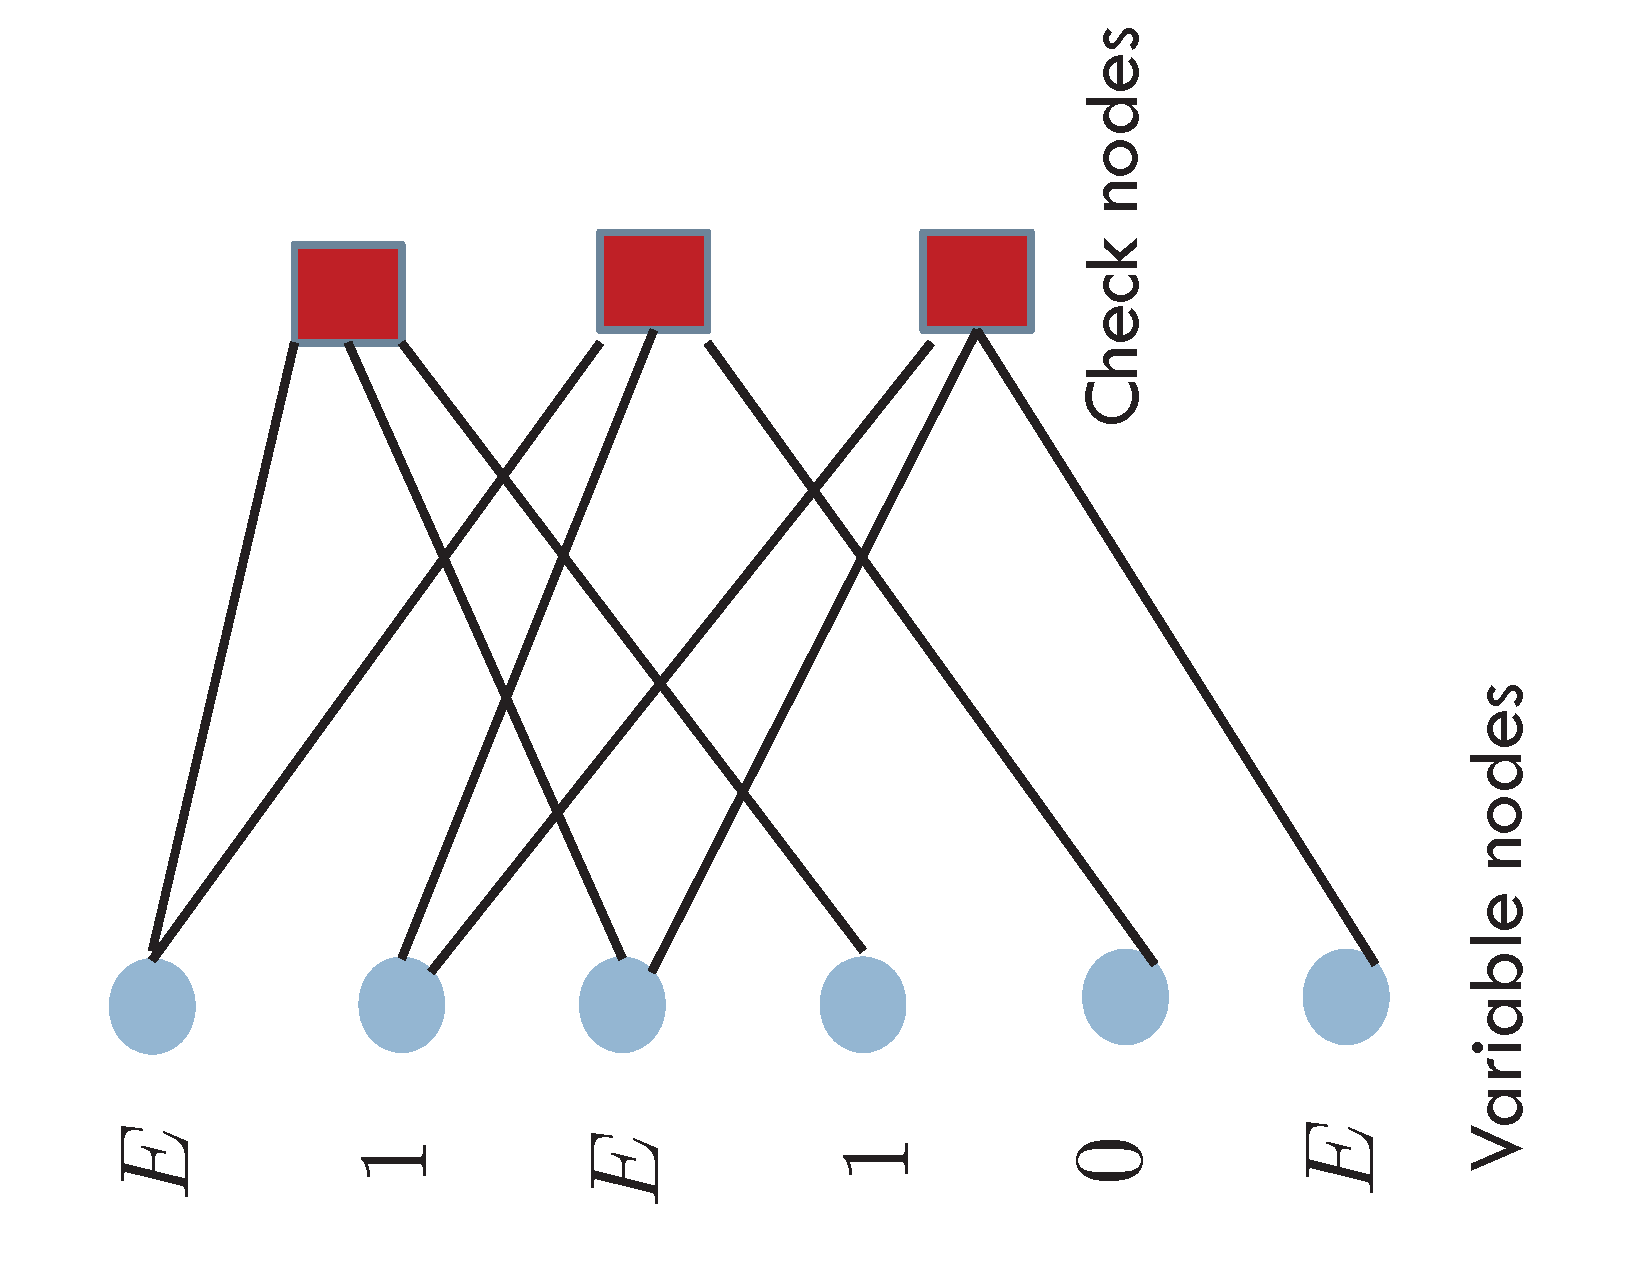
\includegraphics[width=2.25in,angle=-90]{Tannergraph63codewitherasures}
\end{columns}
\vspace{-5mm}
\begin{block}{}
\begin{itemize}
  \item Pass messages between variable nodes and check nodes along the edges
  \item Messages $\in \{\text{value of var node (NE), erasure (E)}\}$
  \item Var-to-check node message is NE if \alert{at least one incoming message is NE}
  \item Check-to-var node message is NE if \alert{all other incoming messages are NE}
\end{itemize}
\end{block}
\end{frame}
%--------------------------------------------------------------------------------------
\begin{frame}{Peeling decoder is a greedy decoder}
\vspace{-3mm}
\begin{columns}
\column{0.5\textwidth}
\[
\Hm = \begin{bmatrix}
      x_1 & x_2 & x_3 & x_4 & x_5 & x_6 \\
      1 & 1 & 1 & 1 & 0 & 0 \\
      1 & 1 & 0 & 0 & 1 & 0 \\
      0 & 1 & 1 & 0 & 0 & 1 \\
    \end{bmatrix}
\]
\begin{eqnarray*}
% \nonumber % Remove numbering (before each equation)
  x_1 \oplus x_2 \oplus x_3 \oplus x_4 &=& 0 \\
  x_1 \oplus x_2 \oplus x_5 &=& 0 \\
  x_2 \oplus x_3 \oplus x_6 &=& 0
\end{eqnarray*}
\column{0.5\textwidth}
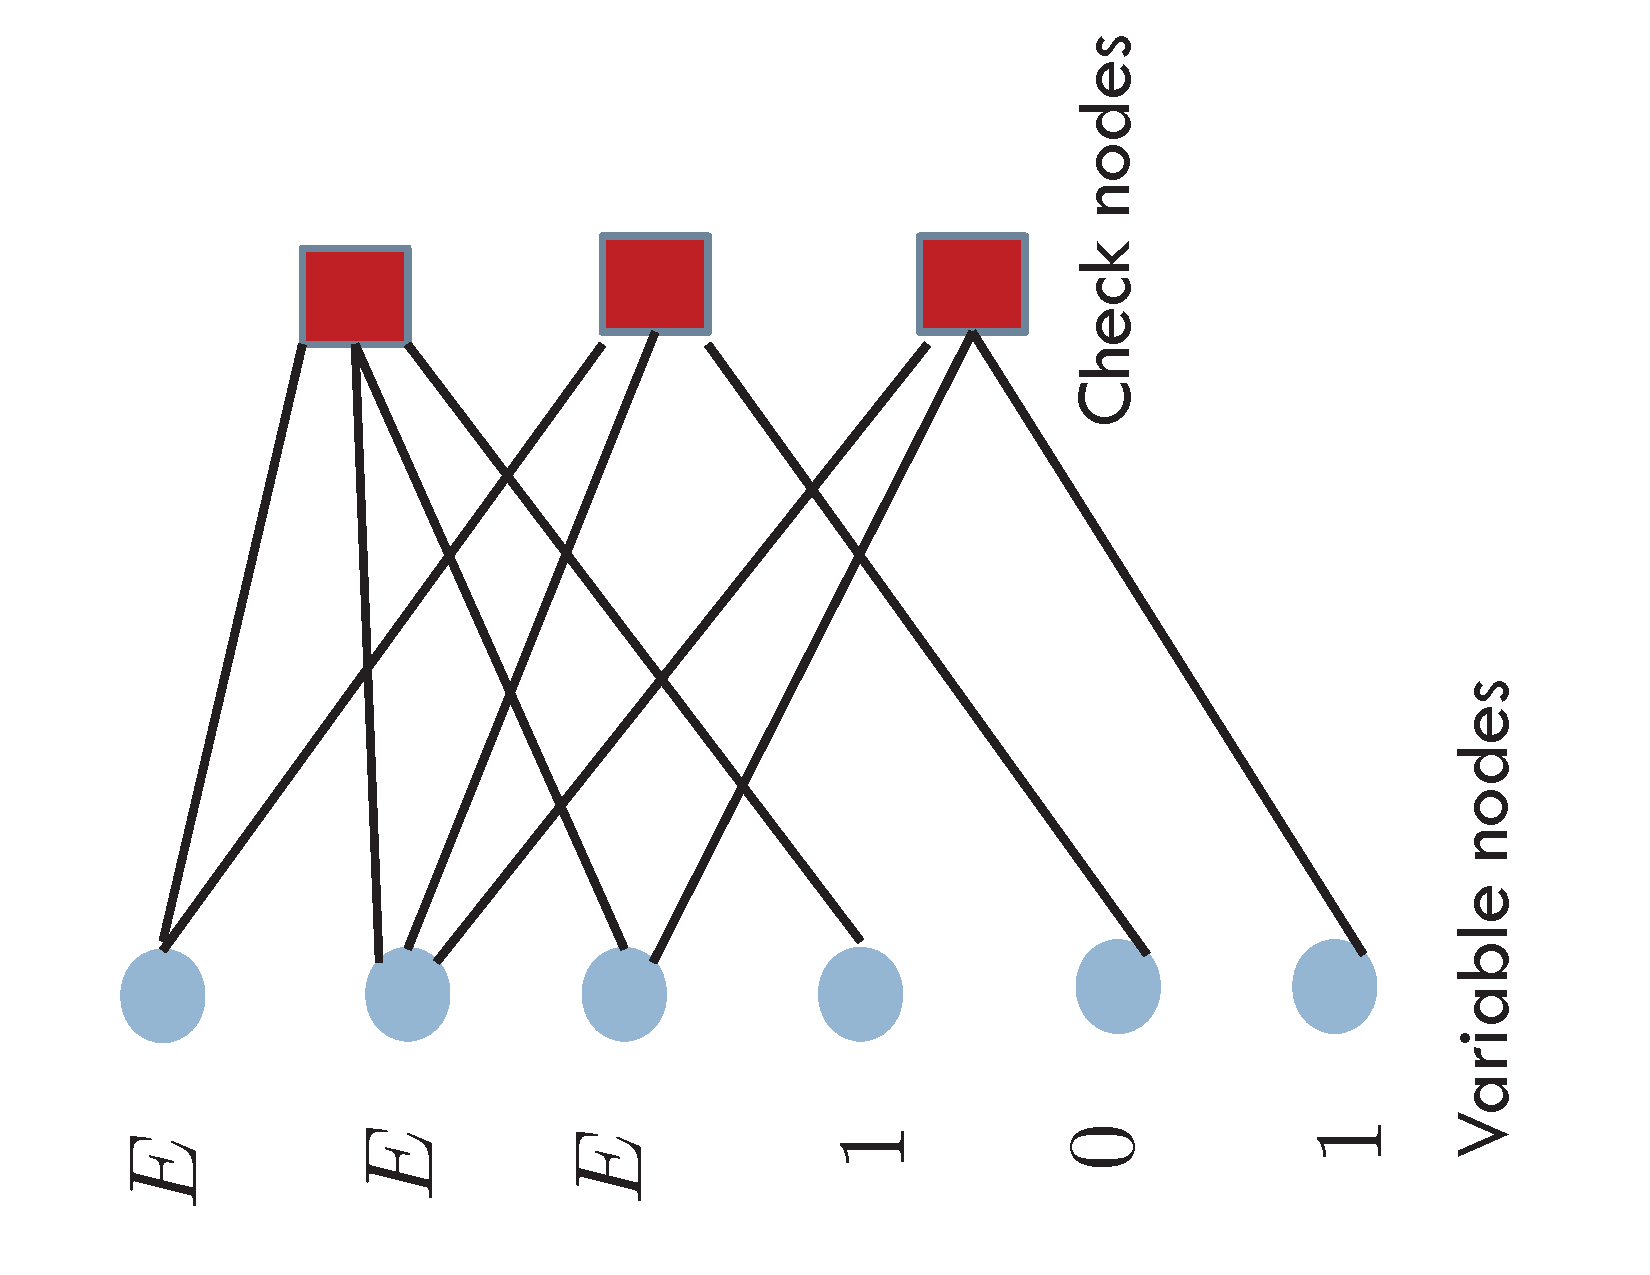
\includegraphics[width=2.25in,angle=-90]{Tannergraph63codestoppingset}
\end{columns}
\pause
\vspace{-3mm}
\begin{columns}
\column{0.5\textwidth}
\begin{block}{Linearly independent set of equations}
\begin{eqnarray*}
% \nonumber % Remove numbering (before each equation)
  x_1 \oplus x_2 \oplus x_3 & = & x_4 \\
  x_1 \oplus x_2  &=& x_5 \\
  x_2 \oplus x_3  &=& x_6
\end{eqnarray*}
\end{block}
\column{0.5\textwidth}
\end{columns}
\end{frame}
%--------------------------------------------------------------------------------------
\begin{frame}{Degree distributions}
\begin{columns}
\begin{column}{0.43\textwidth}
\begin{center}
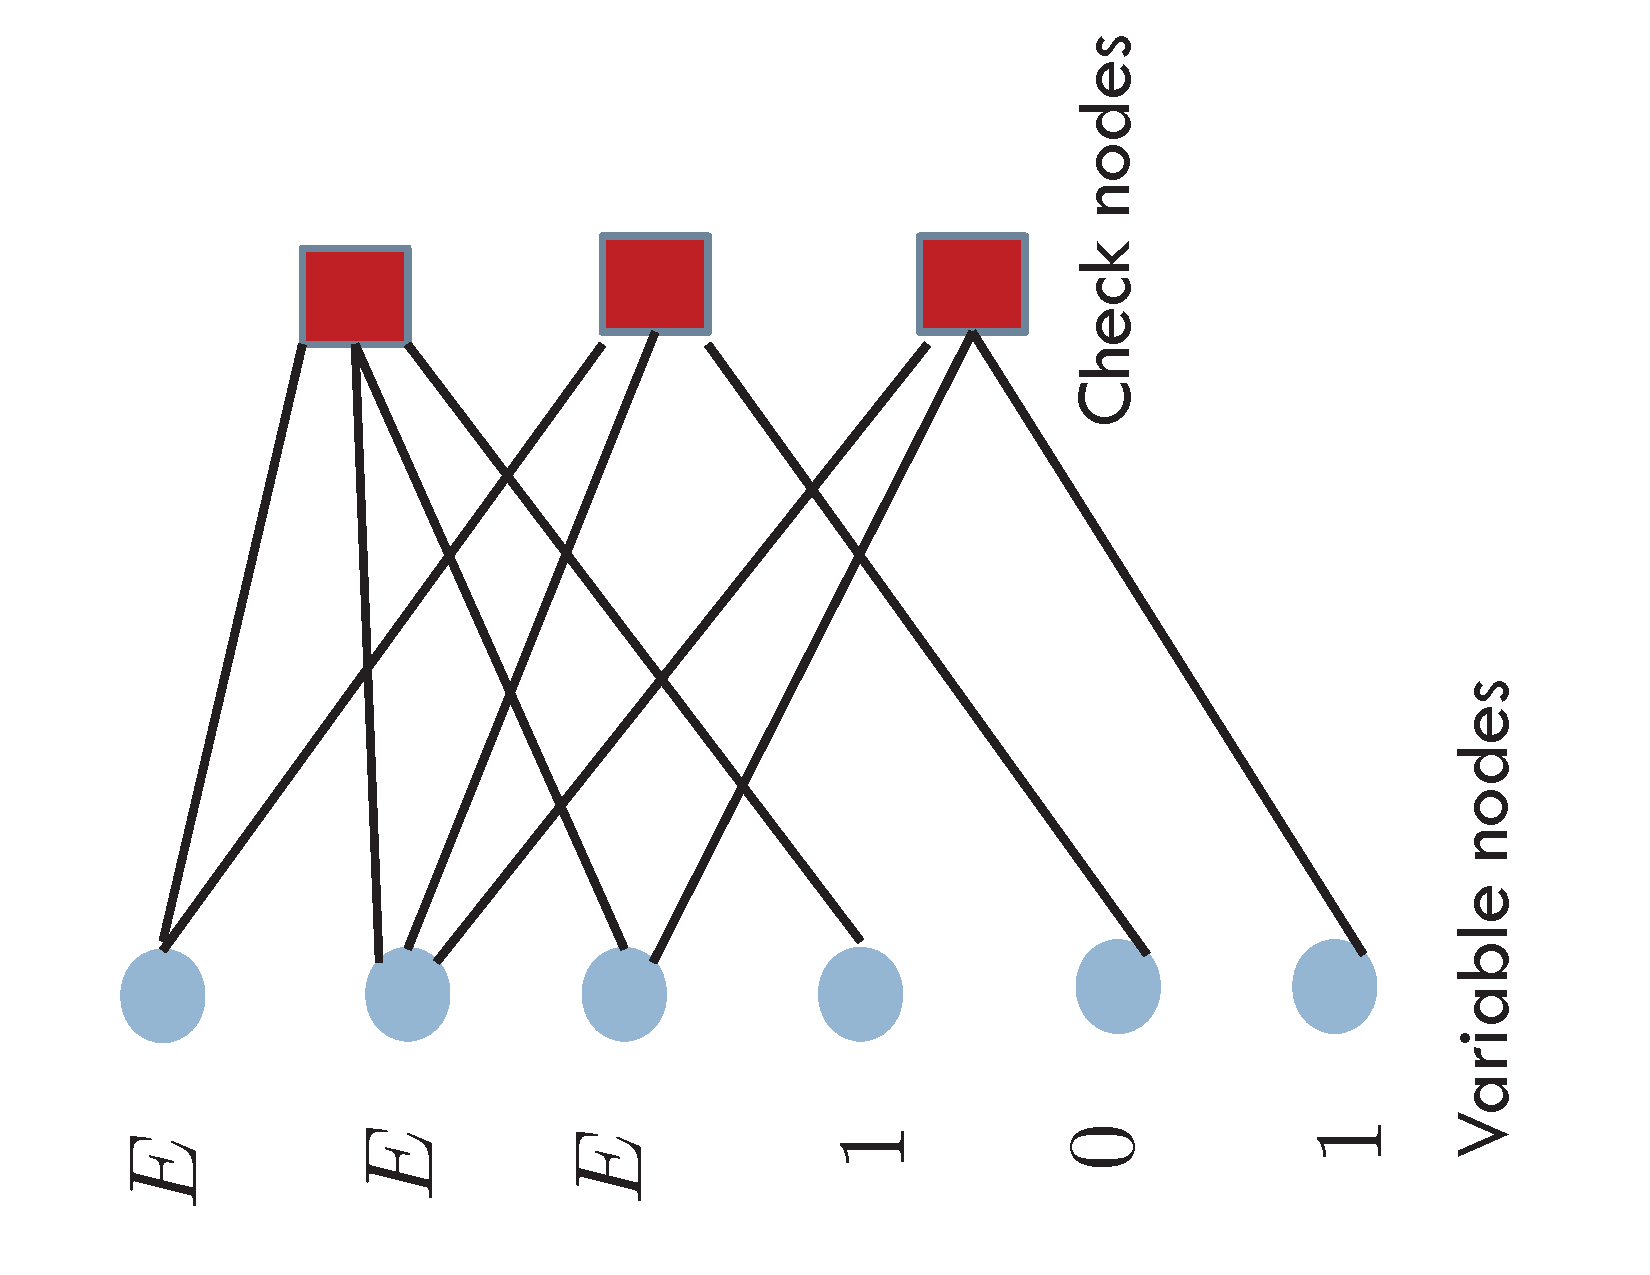
\includegraphics[width=2.0in,angle=-90]{Tannergraph63codestoppingset}
\end{center}
\end{column}
\begin{column}{0.57\textwidth}
\only<5>{
\begin{itemize}
%\item $L(x) = \frac{3}{6} x + \frac26 x^2 + \frac16 x^3$
%\vspace{3mm}
%\item $\lambda(x) = \frac{3}{10} + \frac{4}{10} x + \frac {3}{10} x^2$
%\vspace{3mm}
%\item $R(x) = \frac{2}{3}x^3 + \frac13 x^4$
%\vspace{3mm}
%\item $\rho(x) = \frac{6}{10} x^2+ \frac{4}{10} x^3$
%\item $l_{\text{avg}} = L'(1) = \frac{1}{\int_{0}^{1} \lambda(x) \ dx}$
%\item $r_{\text{avg}} = R'(1) = \frac{1}{\int_{0}^{1} \rho(x) \ dx}$
\item Rate - $r(\lambda,\rho) = 1-\frac{{l_{\text{avg}}}}{{r_{\text{avg}}}} = 1 - \frac{\int_{0}^{1} \rho(x) \ dx}{\int_{0}^{1} \lambda(x) \ dx}$
\end{itemize}
}
\end{column}
\end{columns}

\begin{itemize}
\item VN d.d. from node perspective - $L(x) = \sum_i L_i x^i = \frac{3}{6} x + \frac26 x^2 + \frac16 x^3$
\vspace{1mm}
\pause
\item VN d.d. from edge perspective - $\lambda(x) = \sum_i \lambda_i x^{i-1} = \frac{3}{10} + \frac{4}{10} x + \frac {3}{10} x^2$
\vspace{1mm}
\pause
\item CN d.d. from node perspective - $R(x) = \sum_i R_i x^i = \frac{2}{3}x^3 + \frac13 x^4 $
\vspace{1mm}
\pause
\item CN d.d. from edge perspective - $\rho(x) =\sum_i \rho_i x^{i-1} = \frac{6}{10} x^2+ \frac{4}{10} x^3$
\end{itemize}

\end{frame}
%--------------------------------------------------------------------------------------
\begin{frame}{LDPC code ensemble}
\begin{center}
  %\scalebox{1}{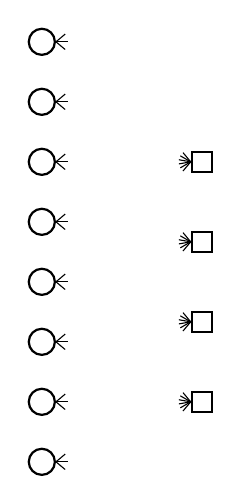
\begin{tikzpicture}
\def\horzgap{0.8in}; %Horizontal gap between nodes/levels
\def \gapVN{0.3in}; %vertical gap between nodes
\def \gapCN{0.4in}; %Horizontal gap between nodes

\def \textoffs{0.12in}; %Offset for writing text above a node
\def\nodewidth{0.1in};
\def\ext{0.06in};



\def \n {8};
\def\ldeg{3};
\def \m {4};
\def\rdeg{6};
\def\langle{40};%120 degrees/3
\def\langle{20};%120 degrees/6

\tikzstyle{check} = [rectangle, draw, text centered, thick, 
                          minimum height=\nodewidth, minimum width=\nodewidth]
\tikzstyle{bit} = [circle, draw, text centered, thick,
                          radius=0.5*\nodewidth]
                          
\foreach \vn in {1,...,\n}{
 \node[bit] (vn\vn) at (0,\vn*\gapVN) {};
 \draw (vn\vn.east) --+ (+40:\ext); 
  \draw (vn\vn.east) --+ (0:\ext); 
   \draw (vn\vn.east) --+ (-40:\ext); 
}


\foreach \cn in {1,...,\m}{
\node[check] (cn\cn) at (\horzgap,0.2in+\cn*\gapCN) {};

 \draw (cn\cn.west) --+ (+130:\ext); 
 \draw (cn\cn.west) --+ (+150:\ext); 
 \draw (cn\cn.west) --+ (+170:\ext); 
 \draw (cn\cn.west) --+ (+190:\ext); 
 \draw (cn\cn.west) --+ (+210:\ext); 
 \draw (cn\cn.west) --+ (+230:\ext); 
}

\end{tikzpicture}}
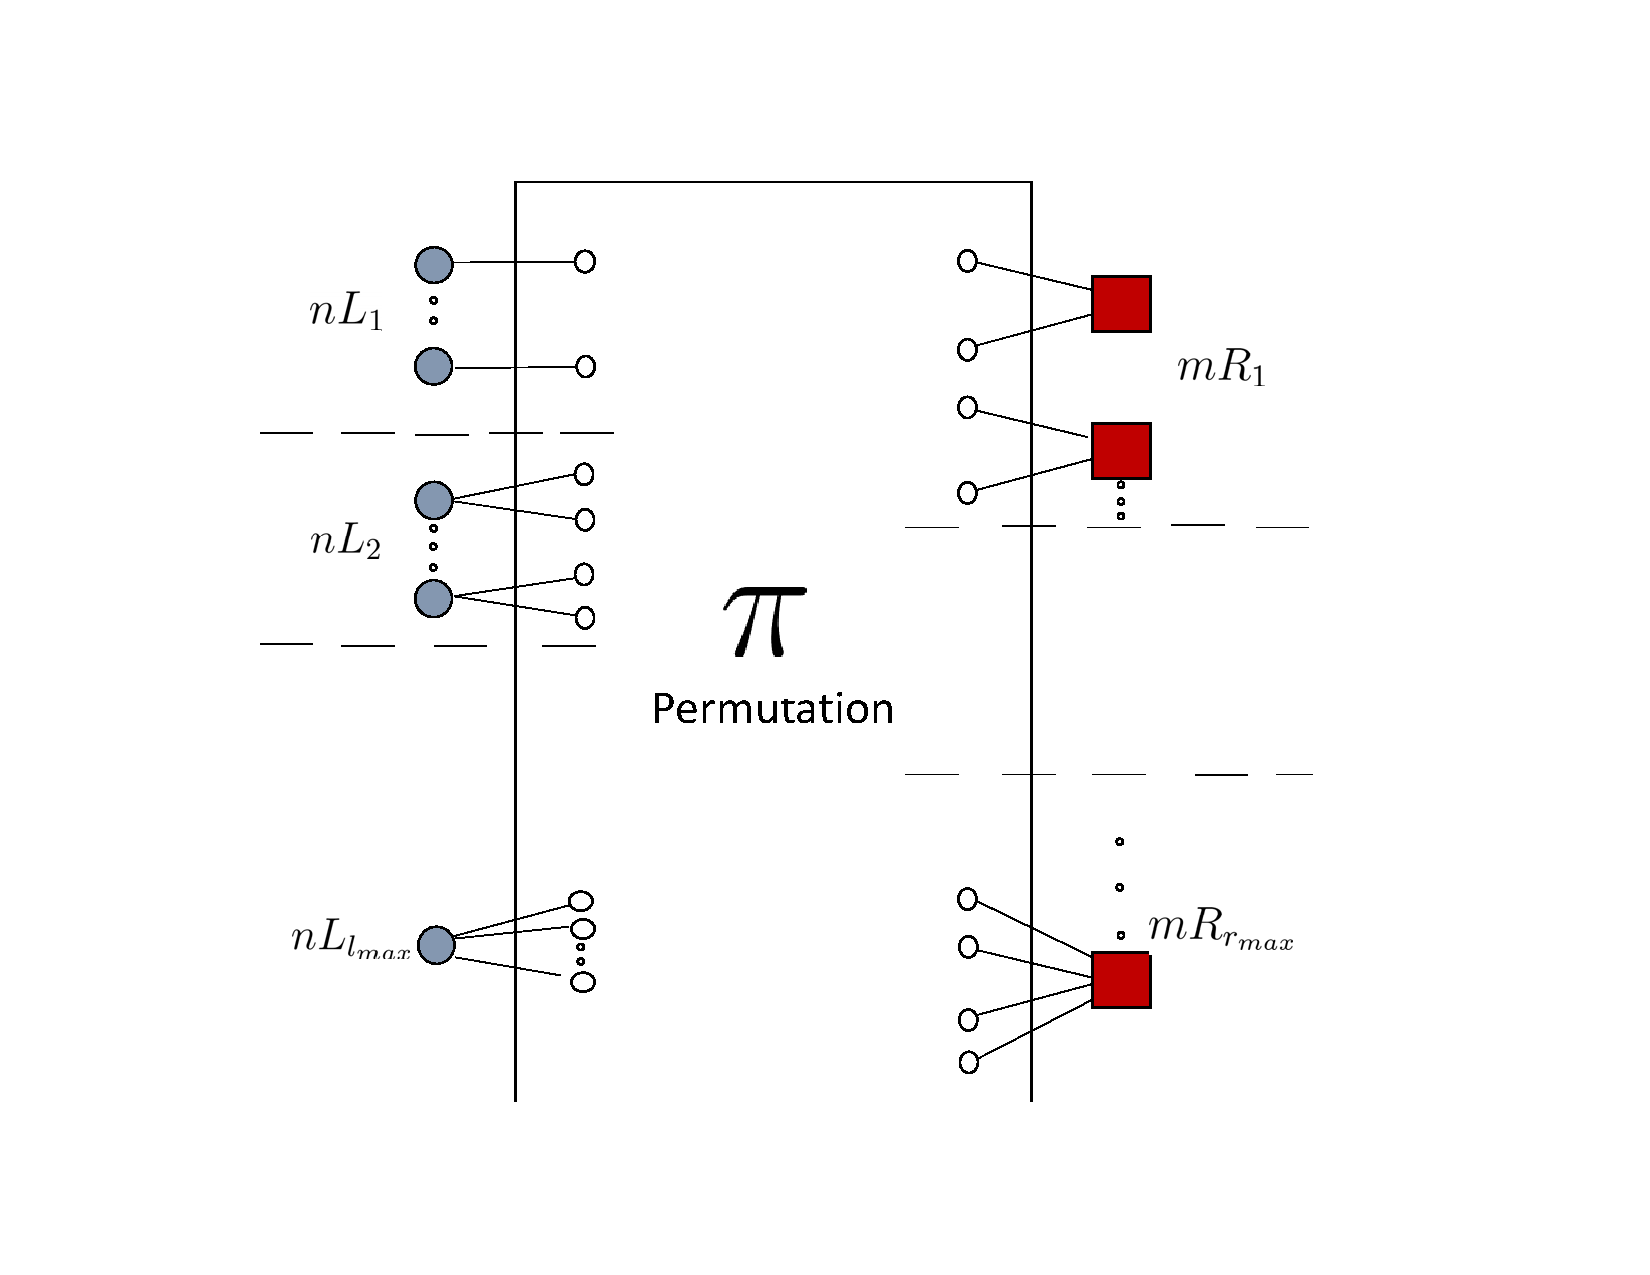
\includegraphics[width=2.2in]{LDPCensemble}
\end{center}
\vspace*{-3mm}
\begin{block}{LDPC($n,\lambda,\rho$) ensemble}
\begin{itemize}
\item Ensemble of codes obtained by using different permutations $\pi$
\item Assume there is only one edge between every var node and check node
\item For every $n$, we get an ensemble of codes with the same $(\lambda,\rho)$
%\item Almost all codes in the ensemble have the same rate
\item \alert{Low density parity check} (LDPC) ensemble if graph is of low density
\end{itemize}
\end{block}
\end{frame}
%%--------------------------------------------------------------------------------------
%\begin{frame}{Rate of the code (ensemble)}
%\begin{itemize}
%  \item $l_{\text{avg}} = L'(1) = \frac{1}{\int_{0}^{1} \lambda(x) \ dx}$
%  \item $r_{\text{avg}} = R'(1) = \frac{1}{\int_{0}^{1} \rho(x) \ dx}$
%  \item Rate $\boxed{r(\lambda,\rho) = 1-\frac{{l_{\text{avg}}}}{{r_{\text{avg}}}} = 1 - \frac{\int_{0}^{1} \rho(x) \ dx}{\int_{0}^{1} \lambda(x) \ dx}}$
%\end{itemize}
%\end{frame}
%--------------------------------------------------------------------------------------
\begin{frame}{Analysis of the message passing decoder}
\begin{block}{}
\begin{itemize}
  \item If we pick a code uniformly at random from the LDPC$(n,\lambda,\rho)$ ensemble and use it over a BEC($\epsilon$) with $l$ iterations of message passing decoding, what will be the probability of erasure $P_{e}^n$ in the limit $l,n \rightarrow \infty$ ?
      \pause
    \begin{itemize}
      \item Analyze the average prob. of erasure over the ensemble
      \item For almost all realizations $P_{e}^n$ concentrates around the average
    \end{itemize}
\end{itemize}
\end{block}
\pause
\begin{block}{Relevant literature}
\begin{itemize}
    \item Papers by Luby, Mitzenmacher, Shokrollahi, Spielman, Stemann 97-'02
    \item Explained in Modern coding theory by Richardson and Urbanke
    \item Henry Pfister's course notes on his webpage
\end{itemize}
\end{block}
\end{frame}
%--------------------------------------------------------------------------------------
\begin{frame}{Analysis of the message passing decoder}
\begin{block}{Computation graph}
Computation graph $\mathcal{C}_{l}(x_1,\lambda,\rho)$ of bit $x_{1}$ of depth $l$ ($l$-iterations) is the neighborhood graph of node $x_1$ of radius $l$. \pause Consider the example $\mathcal{C}_{l=1}(\lambda(x)=x,\rho(x)=x^2)$
\end{block}

\begin{columns}
\begin{column}{0.33\textwidth}
\begin{center}
\scalebox{0.6}{%\documentclass{article}
%
%\usepackage{tikz}
%\usetikzlibrary{arrows,shapes,chains,matrix,positioning,scopes,patterns,calc}
%\usepackage{color}
%
%\usepackage{latexsym}
%\usepackage{amsmath,amssymb,amsthm}
%\usepackage{etoolbox}
%\usetikzlibrary{decorations.pathreplacing} %Big Braces
%\begin{document}

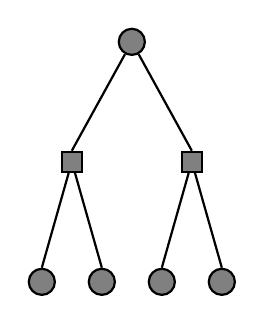
\begin{tikzpicture}
\def \depth{0.6in}; %vertical gap between nodes/levels
\def \gap{0.3in}; %Horizontal gap between nodes
\def \gapA{0.15in}; %Encoder Width
\def \textoffs{0.12in}; %Offset for writing text above a node
\def\nodewidth{0.1in};
\tikzstyle{check} = [rectangle, draw, text centered, thick, fill=gray,
                          minimum height=\nodewidth, minimum width=\nodewidth]
\tikzstyle{bit} = [circle, draw, text centered, thick, fill=gray,
                          radius=0.5*\nodewidth]
                          
\def \fsize{\normalsize}; %Defining a generic font size to be adjusted depending on the scaling
\def \dotsize{\Huge}; %Defining a generic font size to be adjusted depending on the scaling


\node [bit](b1) at (0,0) {} ;

%Level 2
\node[check] (c21) at ([xshift=-\gap,yshift=-\depth]b1) {};
\node[check] (c22) at ([xshift=+\gap,yshift=-\depth]b1) {};

%Lines form level 1-level 2
\draw[thick](b1)--(c21.north);
\draw[thick](b1)--(c22.north);

%Level 3
\node[bit] (b31) at ([xshift=-\gapA,yshift=-\depth]c21) {};
\node[bit] (b32) at ([xshift=+\gapA,yshift=-\depth]c21) {};
\node[bit] (b33) at ([xshift=-\gapA,yshift=-\depth]c22) {};
\node[bit] (b34) at ([xshift=+\gapA,yshift=-\depth]c22) {};

%Lines form level 2-level 3
\draw[thick](c21)--(b31.north);
\draw[thick](c21)--(b32.north);
\draw[thick](c22)--(b33.north);
\draw[thick](c22)--(b34.north);

\end{tikzpicture}
%\end{document}}
%$G_1$\\$Pr(\mathcal{C}_l(x_1)=G_1)=
\\$1-O(1/n)$
\end{center}
\end{column}

\begin{column}{0.33\textwidth}
\begin{center}
\scalebox{0.6}{
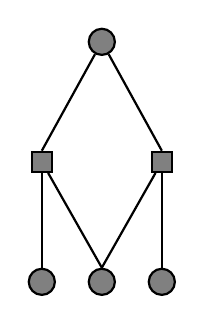
\begin{tikzpicture}
\def \depth{0.6in}; %vertical gap between nodes/levels
\def \gap{0.3in}; %Horizontal gap between nodes
\def \gapA{0.15in}; %Encoder Width
\def \textoffs{0.12in}; %Offset for writing text above a node
\def\nodewidth{0.1in};
\tikzstyle{check} = [rectangle, draw, text centered, thick, fill=gray,
                          minimum height=\nodewidth, minimum width=\nodewidth]
\tikzstyle{bit} = [circle, draw, text centered, thick, fill=gray,
                          radius=0.5*\nodewidth]
                          
\def \fsize{\normalsize}; %Defining a generic font size to be adjusted depending on the scaling
\def \dotsize{\Huge}; %Defining a generic font size to be adjusted depending on the scaling


\node [bit](b1) at (0,0) {} ;

%Level 2
\node[check] (c21) at ([xshift=-\gap,yshift=-\depth]b1) {};
\node[check] (c22) at ([xshift=+\gap,yshift=-\depth]b1) {};

%Lines form level 1-level 2
\draw[thick](b1)--(c21.north);
\draw[thick](b1)--(c22.north);

%Level 3
\node[bit] (b31) at ([xshift=0,yshift=-\depth]c21) {};
\node[bit] (b32) at ([xshift=+\gap,yshift=-\depth]c21) {};
\node[bit] (b33) at ([xshift=0,yshift=-\depth]c22) {};

%Lines form level 2-level 3
\draw[thick](c21)--(b31.north);
\draw[thick](c21)--(b32.north);
\draw[thick](c22)--(b33.north);
\draw[thick](c22)--(b32.north);

\end{tikzpicture}}
%$G_2$\\ \scriptsize{$Pr(\mathcal{C}_l(x_1)=G_2)=O(1/n)$}
\\$O(1/n)$
\end{center}
\end{column}

\begin{column}{0.33\textwidth}
\begin{center}
\scalebox{0.6}{
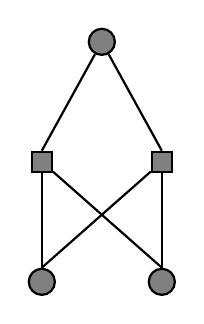
\begin{tikzpicture}
\def \depth{0.6in}; %vertical gap between nodes/levels
\def \gap{0.3in}; %Horizontal gap between nodes
\def \gapA{0.15in}; %Encoder Width
\def \textoffs{0.12in}; %Offset for writing text above a node
\def\nodewidth{0.1in};
\tikzstyle{check} = [rectangle, draw, text centered, thick, fill=gray,
                          minimum height=\nodewidth, minimum width=\nodewidth]
\tikzstyle{bit} = [circle, draw, text centered, thick, fill=gray,
                          radius=0.5*\nodewidth]
                          
\def \fsize{\normalsize}; %Defining a generic font size to be adjusted depending on the scaling
\def \dotsize{\Huge}; %Defining a generic font size to be adjusted depending on the scaling


\node [bit](b1) at (0,0) {} ;

%Level 2
\node[check] (c21) at ([xshift=-\gap,yshift=-\depth]b1) {};
\node[check] (c22) at ([xshift=+\gap,yshift=-\depth]b1) {};

%Lines form level 1-level 2
\draw[thick](b1)--(c21.north);
\draw[thick](b1)--(c22.north);

%Level 3
\node[bit] (b31) at ([yshift=-\depth]c21) {};
\node[bit] (b32) at ([yshift=-\depth]c22) {};

%Lines form level 2-level 3
\draw[thick](c21)--(b31.north);
\draw[thick](c21)--(b32.north);
\draw[thick](c22)--(b31.north);
\draw[thick](c22)--(b32.north);

\end{tikzpicture}}
%$G_3$\\ $Pr(\mathcal{C}_l(x_1)=G_3)=O(1/n^2)$
\\$O(1/n^2)$
\end{center}
\end{column}

\end{columns}
\pause
\begin{block}{Computation tree}
For fixed $(l_{max},r_{max})$, in the limit of large block lengths a computation graph of depth-$l$ looks like a tree with high probability
\end{block}
\end{frame}
%--------------------------------------------------------------------------------------
\begin{frame}{Analysis of the message passing decoder}

\begin{block}{Computation Tree Ensemble-$\mathcal{T}_{l}(\lambda,\rho)$}
Ensemble of bipartite trees of depth $l$ rooted in a variable node (VN) where
\begin{itemize}
\item Root node has $i$ children(CN's) with probability $L_i$
\item Each VN has $i$ children(CN's) with probability $\lambda_i$
\item Each CN has $i$ children(VN's) with probability $\rho_i$
\end{itemize}
\end{block}

\begin{block}{Example: $\mathcal{C}_{l=1}(\lambda(x)=x,\rho(x)=x^2)$}
\begin{center}
\scalebox{0.6}{%\documentclass{article}
%
%\usepackage{tikz}
%\usetikzlibrary{arrows,shapes,chains,matrix,positioning,scopes,patterns,calc}
%\usepackage{color}
%
%\usepackage{latexsym}
%\usepackage{amsmath,amssymb,amsthm}
%\usepackage{etoolbox}
%\usetikzlibrary{decorations.pathreplacing} %Big Braces
%\begin{document}

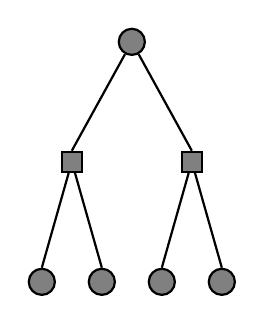
\begin{tikzpicture}
\def \depth{0.6in}; %vertical gap between nodes/levels
\def \gap{0.3in}; %Horizontal gap between nodes
\def \gapA{0.15in}; %Encoder Width
\def \textoffs{0.12in}; %Offset for writing text above a node
\def\nodewidth{0.1in};
\tikzstyle{check} = [rectangle, draw, text centered, thick, fill=gray,
                          minimum height=\nodewidth, minimum width=\nodewidth]
\tikzstyle{bit} = [circle, draw, text centered, thick, fill=gray,
                          radius=0.5*\nodewidth]
                          
\def \fsize{\normalsize}; %Defining a generic font size to be adjusted depending on the scaling
\def \dotsize{\Huge}; %Defining a generic font size to be adjusted depending on the scaling


\node [bit](b1) at (0,0) {} ;

%Level 2
\node[check] (c21) at ([xshift=-\gap,yshift=-\depth]b1) {};
\node[check] (c22) at ([xshift=+\gap,yshift=-\depth]b1) {};

%Lines form level 1-level 2
\draw[thick](b1)--(c21.north);
\draw[thick](b1)--(c22.north);

%Level 3
\node[bit] (b31) at ([xshift=-\gapA,yshift=-\depth]c21) {};
\node[bit] (b32) at ([xshift=+\gapA,yshift=-\depth]c21) {};
\node[bit] (b33) at ([xshift=-\gapA,yshift=-\depth]c22) {};
\node[bit] (b34) at ([xshift=+\gapA,yshift=-\depth]c22) {};

%Lines form level 2-level 3
\draw[thick](c21)--(b31.north);
\draw[thick](c21)--(b32.north);
\draw[thick](c22)--(b33.north);
\draw[thick](c22)--(b34.north);

\end{tikzpicture}
%\end{document}}
\end{center}
\end{block}

\end{frame}
%---------------------------------------------------------------------------------------------------------------------------
\begin{frame}{Density evolution}
\begin{columns}
\begin{column}{0.65\textwidth}
\begin{centering}
\scalebox{0.73}{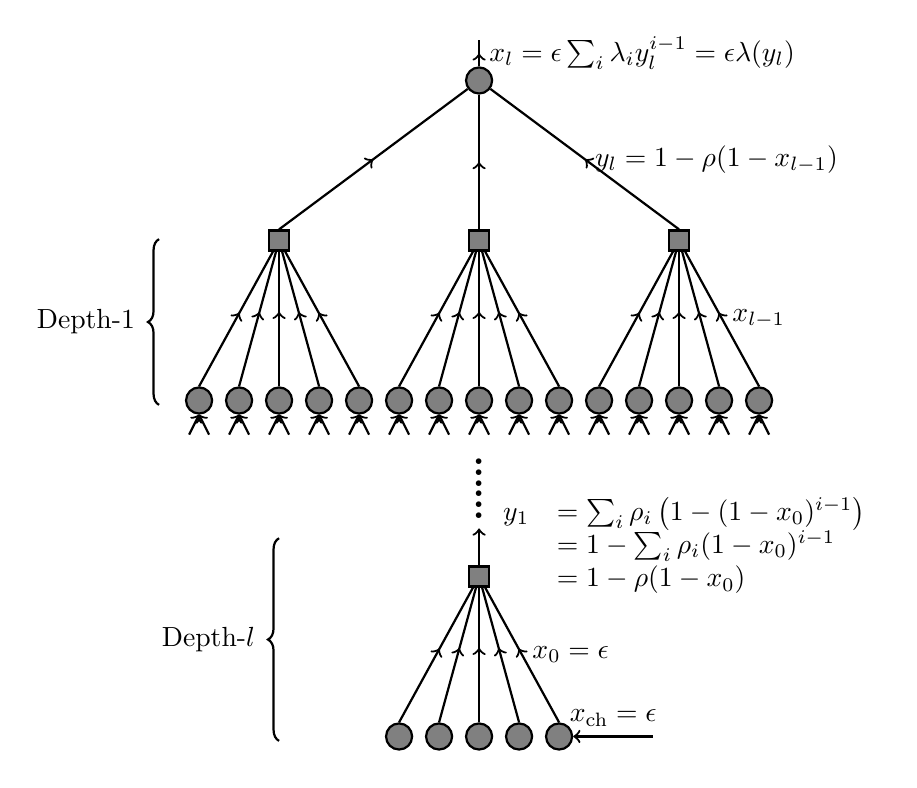
\begin{tikzpicture}
\def \depth{0.8in}; %Encoder Length
\def \gap{1in}; %Encoder Width
\def \gapA{0.2in}; %Encoder Width
\def\nodewidth{0.1in};
\tikzstyle{check} = [rectangle, draw, text centered, thick,fill=gray,
                          minimum height=\nodewidth, minimum width=\nodewidth]
\tikzstyle{bit} = [circle, draw, text centered, thick,fill=gray,
                          radius=0.5*\nodewidth]

\def \fsize{\normalsize}; %Defining a generic font size to be adjusted depending on the scaling
\def \dotsize{\Huge}; %Defining a generic font size to be adjusted depending on the scaling

\node [bit](b1) at (0,0) {} ;
%\node() at ([yshift=0.12in]b1) {$x_{\text{DE}}^{(l)}=\epsilon \sum_{i} \lambda y_l^{i-1}$ };

%Level 2
\node[check] (c21) at ([xshift=-\gap,yshift=-\depth]b1) {};
\node[check] (c22) at ([yshift=-\depth]b1) {};
\node[check] (c23) at ([xshift=+\gap,yshift=-\depth]b1) {};

%Lines form level 1-level 2
\begin{scope}[thick,decoration={
    markings,
    mark=at position 0.5 with {\arrow{>}}}
    ]
\draw[postaction={decorate}] (b1)--+(0,+0.2in)node[midway,right]{$x_{l}=\epsilon \sum_{i} \lambda_i y_l^{i-1} = \epsilon \lambda(y_l)$ };
\draw[postaction={decorate}](c21.north)--(b1);
\draw[postaction={decorate}](c22)--(b1);
\draw[postaction={decorate}](c23.north)--(b1)node[midway,right]{$y_{l}=1-\rho(1- x_{l-1})$};
\end{scope}

%Level 3
\node[bit] (b31) at ([xshift=-2*\gapA,yshift=-\depth]c21) {};
\node[bit] (b32) at ([xshift=-\gapA,yshift=-\depth]c21) {};
\node[bit] (b33) at ([yshift=-\depth]c21) {};
\node[bit] (b34) at ([xshift=+\gapA,yshift=-\depth]c21) {};
\node[bit] (b35) at ([xshift=2*\gapA,yshift=-\depth]c21) {};

\node[bit] (b36) at ([xshift=-2*\gapA,yshift=-\depth]c22) {};
\node[bit] (b37) at ([xshift=-\gapA,yshift=-\depth]c22) {};
\node[bit] (b38) at ([yshift=-\depth]c22) {};
\node[bit] (b39) at ([xshift=+\gapA,yshift=-\depth]c22) {};
\node[bit] (b310) at ([xshift=2*\gapA,yshift=-\depth]c22) {};

\node[bit] (b311) at ([xshift=-2*\gapA,yshift=-\depth]c23) {};
\node[bit] (b312) at ([xshift=-\gapA,yshift=-\depth]c23) {};
\node[bit] (b313) at ([yshift=-\depth]c23) {};
\node[bit] (b314) at ([xshift=+\gapA,yshift=-\depth]c23) {};
\node[bit] (b315) at ([xshift=2*\gapA,yshift=-\depth]c23) {};


%Lines form level 2-level 3
\begin{scope}[thick,decoration={
    markings,
    mark=at position 0.5 with {\arrow{<}}}
    ]
\draw[postaction={decorate}](c21)--(b31.north);
\draw[postaction={decorate}](c21)--(b32.north);
\draw[postaction={decorate}](c21)--(b33.north);
\draw[postaction={decorate}](c21)--(b34.north);
\draw[postaction={decorate}](c21)--(b35.north);

\draw[postaction={decorate}](c22)--(b36.north);
\draw[postaction={decorate}](c22)--(b37.north);
\draw[postaction={decorate}](c22)--(b38.north);
\draw[postaction={decorate}](c22)--(b39.north);
\draw[postaction={decorate}](c22)--(b310.north);

\draw[postaction={decorate}](c23)--(b311.north);
\draw[postaction={decorate}](c23)--(b312.north);
\draw[postaction={decorate}](c23)--(b313.north);
\draw[postaction={decorate}](c23)--(b314.north);
\draw[postaction={decorate}](c23)--(b315.north)node[midway,right]{$x_{l-1}$};%=\epsilon \sum_i \lmb_i y_l^{i-1}  $};
\end{scope}


\node(brace11) at ([xshift=-0.6in]c21.north){};
\node(brace12) at ([xshift=-0.6in]b33.south){};
\draw [decorate,thick,decoration={brace,amplitude=4pt,mirror}](brace11) -- (brace12) node [black,midway,left,xshift=-5pt]{\fsize Depth-$1$};

 \node (dots1) at ([yshift=-0.4*\depth]b38){\dotsize $\vdots$};
\node (dots2) at ([yshift=-0.6*\depth]b38){\dotsize $\vdots$};


%Lines form level 3-level 4
\def \offsx{0.05in};
\def \offsy{0.1in};
\draw[->,thick](b31.south)+(-\offsx,-\offsy)--(b31.south); \draw[->,thick](b31.south)+(\offsx,-\offsy)--(b31.south);
\draw[->,thick](b32.south)+(-\offsx,-\offsy)--(b32.south); \draw[->,thick](b32.south)+(\offsx,-\offsy)--(b32.south);
\draw[->,thick](b33.south)+(-\offsx,-\offsy)--(b33.south); \draw[->,thick](b33.south)+(\offsx,-\offsy)--(b33.south);
\draw[->,thick](b34.south)+(-\offsx,-\offsy)--(b34.south); \draw[->,thick](b34.south)+(\offsx,-\offsy)--(b34.south);
\draw[->,thick](b35.south)+(-\offsx,-\offsy)--(b35.south); \draw[->,thick](b35.south)+(\offsx,-\offsy)--(b35.south);
\draw[->,thick](b36.south)+(-\offsx,-\offsy)--(b36.south); \draw[->,thick](b36.south)+(\offsx,-\offsy)--(b36.south);
\draw[->,thick](b37.south)+(-\offsx,-\offsy)--(b37.south); \draw[->,thick](b37.south)+(\offsx,-\offsy)--(b37.south);
\draw[->,thick](b38.south)+(-\offsx,-\offsy)--(b38.south); \draw[->,thick](b38.south)+(\offsx,-\offsy)--(b38.south);
\draw[->,thick](b39.south)+(-\offsx,-\offsy)--(b39.south); \draw[->,thick](b39.south)+(\offsx,-\offsy)--(b39.south);
\draw[->,thick](b310.south)+(-\offsx,-\offsy)--(b310.south); \draw[->,thick](b310.south)+(\offsx,-\offsy)--(b310.south);
\draw[->,thick](b311.south)+(-\offsx,-\offsy)--(b311.south); \draw[->,thick](b311.south)+(\offsx,-\offsy)--(b311.south);
\draw[->,thick](b312.south)+(-\offsx,-\offsy)--(b312.south); \draw[->,thick](b312.south)+(\offsx,-\offsy)--(b312.south);
\draw[->,thick](b313.south)+(-\offsx,-\offsy)--(b313.south); \draw[->,thick](b313.south)+(\offsx,-\offsy)--(b313.south);
\draw[->,thick](b314.south)+(-\offsx,-\offsy)--(b314.south); \draw[->,thick](b314.south)+(\offsx,-\offsy)--(b314.south);
\draw[->,thick](b315.south)+(-\offsx,-\offsy)--(b315.south); \draw[->,thick](b315.south)+(\offsx,-\offsy)--(b315.south);

%Level l
\node[check] (cL1) at ([yshift=-0.5*\depth]dots2) {};

\draw[<-,thick](dots2.south)--(cL1.north)node[midway,right]{$\begin{array}{ll}y_{1}& = \sum_i \rho_i \left(1-(1-x_0)^{i-1} \right)\\
& = 1-\sum_i \rho_i (1-x_0)^{i-1} \\ & = 1-\rho(1-x_{0})\end{array}$};;

%Level l+1
\node[bit] (bl1) at ([xshift=-2*\gapA,yshift=-\depth]cL1) {};
\node[bit] (bl2) at ([xshift=-\gapA,yshift=-\depth]cL1) {};
\node[bit] (bl3) at ([yshift=-\depth]cL1) {};
\node[bit] (bl4) at ([xshift=\gapA,yshift=-\depth]cL1) {};
\node[bit] (bl5) at ([xshift=2*\gapA,yshift=-\depth]cL1) {};


%Lines form level l-level l+1
\begin{scope}[thick,decoration={
    markings,
    mark=at position 0.5 with {\arrow{<}}}
    ]
\draw[postaction={decorate}](cL1)--(bl1.north);
\draw[postaction={decorate}](cL1)--(bl2.north);
\draw[postaction={decorate}](cL1)--(bl3.north);
\draw[postaction={decorate}](cL1)--(bl4.north);
\draw[postaction={decorate}](cL1)--(bl5.north)node[midway,right]{$x_{0}=\epsilon$};
\end{scope}

\draw[<-,thick](bl5.east)--+(2*\gapA,0)node[midway,above]{$x_{\text{ch}}=\epsilon$};


\node(lbrace1) at ([xshift=-1in]dots2.south){};
\node(lbrace2) at ([xshift=-1in]bl3.south){};
\draw [decorate,thick,decoration={brace,amplitude=4pt,mirror}](lbrace1) -- (lbrace2) node [black,midway,left,xshift=-5pt]{\fsize Depth-$l$};


%\draw[<-,thick](enc)-- +(-\ext,0) node[midway,above]{\fsize $m_1,\ldots,m_l$};
%\draw[<-,thick](enc)--(chan)node[midway,above]{\fsize $c_1,\ldots,c_l$}node[midway,below]{\fsize $c_i\in \mathbb{F}_p$};
%\draw[<-,thick](chan)--(dec)node[midway,above]{\fsize $r_1,\ldots,r_l$}node[midway,below]{\fsize $r_i\in \mathbb{F}_p$};;
%
%\draw[<-,thick](chan)--+(0,\extB) node[above] {\fsize $e_1,\ldots,e_l$};
%\draw[<-,thick](dec)--+(\ext,0)node[midway,above]{\fsize  $\hat{m_1},\ldots,\hat{m_l}$};
%
\end{tikzpicture} }
\end{centering}
\end{column}

\begin{column}{0.35\textwidth}
\begin{block}{Recall}
\begin{itemize}
  \item $\rho(x) = \sum_{i} \rho_i x^{i-1}$
  \item $\sum_i \rho_i = 1$
  \item $\lambda(x) = \sum_{i} \lambda_i x^{i-1}$
  \item $\sum_i \lambda_i = 1$
\end{itemize}
\end{block}
\begin{block}{Recursion}
\begin{eqnarray*}
  x_0 &=& \epsilon \\
\pause
  y_l &=& 1-\rho(1-x_{l-1}) \\
\pause
  x_l &=& \epsilon \lambda(y_l)\\
\pause
  x_l &=& \epsilon \lambda(1-\rho(1-x_{l-1}))
\end{eqnarray*}
\end{block}
\end{column}
\end{columns}
\end{frame}
%--------------------------------------------------------------------------------------
\begin{frame}{Analysis of the message passing decoder}
$\lambda(x)=x^2,\rho(x)=\rho_4 x^3+\rho_5 x^4$
\begin{columns}
\only<1,4>{
\begin{column}{0.33\textwidth}
\begin{center}
\scalebox{0.65}{
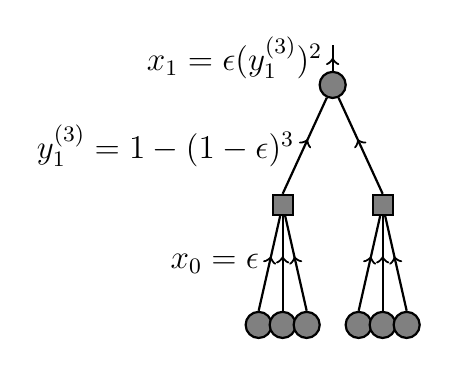
\begin{tikzpicture}
\def \depth{0.6in}; %vertical gap between nodes/levels
\def \gap{0.25in}; %Horizontal gap between nodes
\def \gapA{0.12in}; %Encoder Width
\def \textoffs{0.18in}; %Offset for writing text above a node
\def\nodewidth{0.1in};
\tikzstyle{check} = [rectangle, draw, text centered, thick, fill=gray,
                          minimum height=\nodewidth, minimum width=\nodewidth]
\tikzstyle{bit} = [circle, draw, text centered, thick, fill=gray,
                          radius=0.5*\nodewidth]
                          
\def \fsize{\large}; %Defining a generic font size to be adjusted depending on the scaling
\def \dotsize{\Huge}; %Defining a generic font size to be adjusted depending on the scaling


\node [bit](b1) at (0,0) {} ;
\begin{scope}[thick,decoration={
    markings,
    mark=at position 0.5 with {\arrow{>}}}
    ] 
\draw[postaction={decorate}](b1)--+(0,0.2in)node[midway,left]{\fsize{$x_{1}=\epsilon (y_1^{(3)})^2$}};
\end{scope}


%Level 2
\node[check] (c21) at ([xshift=-\gap,yshift=-\depth]b1) {};
\node[check] (c22) at ([xshift=+\gap,yshift=-\depth]b1) {};

%Lines form level 1-level 2
\begin{scope}[thick,decoration={
    markings,
    mark=at position 0.5 with {\arrow{<}}}
    ] 
\draw[postaction={decorate}](b1)--(c21.north)node[midway,left,align=left]{\fsize{$y_{1}^{(3)}=1-(1-\epsilon)^3$}};
%\draw[postaction={decorate}](b1)--(c21.north)node[midway,left,align=left]{\fsize{$y_{1}^{(3)}=$}\\ \fsize{$1-(1-\epsilon)^3$}};
\draw[postaction={decorate}](b1)--(c22.north);
\end{scope}
%    \draw[postaction={decorate}] (-4,2)--(-4,0);
%\draw[thick](b1)--(c21.north);
%\draw[thick](b1)--(c22.north);

%Level 3
\node[bit] (b31) at ([xshift=-\gapA,yshift=-\depth]c21) {};
\node[bit] (b32) at ([xshift=0,yshift=-\depth]c21) {};
\node[bit] (b33) at ([xshift=+\gapA,yshift=-\depth]c21) {};
\node[bit] (b34) at ([xshift=-\gapA,yshift=-\depth]c22) {};
\node[bit] (b35) at ([xshift=0,yshift=-\depth]c22) {};
\node[bit] (b36) at ([xshift=+\gapA,yshift=-\depth]c22) {};

%Lines form level 2-level 3
\begin{scope}[thick, decoration={
    markings,
    mark=at position 0.5 with {\arrow{<}}}
    ] 
\draw[postaction={decorate}](c21)--(b31.north)node[midway,left]{\fsize{$x_{0}=\epsilon$}};
\draw[postaction={decorate}](c21)--(b32.north);
\draw[postaction={decorate}](c21)--(b33.north); 
\draw[postaction={decorate}](c22)--(b34.north);
\draw[postaction={decorate}](c22)--(b35.north);
\draw[postaction={decorate}](c22)--(b36.north); 
\end{scope}
%\draw[thick](c21)--(b32.north);
%\draw[thick](c21)--(b33.north);
%\draw[thick](c22)--(b34.north);
%\draw[thick](c22)--(b35.north);
%\draw[thick](c22)--(b36.north); 



\end{tikzpicture}}
\\ \scriptsize{$P(T)=\rho_4^2$}
%\\ \scriptsize{$P(T\in\mathcal{T}_1(\lambda,\rho))=\rho_4^2$}
\end{center}
\end{column}
}
\only<2,4>{
\begin{column}{0.33\textwidth}
\begin{center}
\scalebox{0.65}{
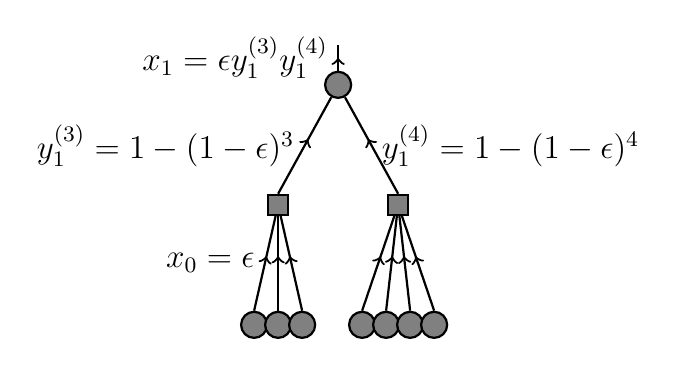
\begin{tikzpicture}
\def \depth{0.6in}; %vertical gap between nodes/levels
\def \gap{0.3in}; %Horizontal gap between nodes
\def \gapA{0.12in}; %Encoder Width
\def \gapB{0.12in}; %Encoder Width
\def \textoffs{0.18in}; %Offset for writing text above a node
\def\nodewidth{0.1in};
\tikzstyle{check} = [rectangle, draw, text centered, thick, fill=gray,
                          minimum height=\nodewidth, minimum width=\nodewidth]
\tikzstyle{bit} = [circle, draw, text centered, thick, fill=gray,
                          radius=0.5*\nodewidth]
                          
\def \fsize{\large}; %Defining a generic font size to be adjusted depending on the scaling
\def \dotsize{\Huge}; %Defining a generic font size to be adjusted depending on the scaling


\node [bit](b1) at (0,0) {} ;
\begin{scope}[thick,decoration={
    markings,
    mark=at position 0.5 with {\arrow{>}}}
    ] 
\draw[postaction={decorate}](b1)--+(0,0.2in)node[midway,left]{\fsize{$x_{1}=\epsilon y_1^{(3)}y_1^{(4)}$}};
\end{scope}

%Level 2
\node[check] (c21) at ([xshift=-\gap,yshift=-\depth]b1) {};
\node[check] (c22) at ([xshift=+\gap,yshift=-\depth]b1) {};

%Lines form level 1-level 2
\begin{scope}[thick,decoration={
    markings,
    mark=at position 0.5 with {\arrow{<}}}
    ] 
\draw[postaction={decorate}](b1)--(c21.north)node[midway,left,align=left]{\fsize{$y_{1}^{(3)}=1-(1-\epsilon)^3$}};
\draw[postaction={decorate}](b1)--(c22.north)node[midway,right,align=left]{\fsize{$y_{1}^{(4)}=1-(1-\epsilon)^4$}};
%\draw[postaction={decorate}](b1)--(c21.north)node[midway,left,align=left]{\fsize{$y_{1}^{(3)}=$} \\ \fsize{$1-(1-\epsilon)^3$}};
%\draw[postaction={decorate}](b1)--(c22.north)node[midway,right,align=left]{\fsize{$y_{1}^{(4)}=$} \\ \fsize{$1-(1-\epsilon)^4$}};
\end{scope}
%    \draw[postaction={decorate}] (-4,2)--(-4,0);
%\draw[thick](b1)--(c21.north);
%\draw[thick](b1)--(c22.north);

%Level 3
\node[bit] (b31) at ([xshift=-\gapA,yshift=-\depth]c21) {};
\node[bit] (b32) at ([xshift=0,yshift=-\depth]c21) {};
\node[bit] (b33) at ([xshift=+\gapA,yshift=-\depth]c21) {};
\node[bit] (b34) at ([xshift=-0.18in,yshift=-\depth]c22) {};
\node[bit] (b35) at ([xshift=-0.06in,yshift=-\depth]c22) {};
\node[bit] (b36) at ([xshift=+0.06in,yshift=-\depth]c22) {};
\node[bit] (b37) at ([xshift=+0.18in,yshift=-\depth]c22) {};

%Lines form level 2-level 3
\begin{scope}[thick, decoration={
    markings,
    mark=at position 0.5 with {\arrow{<}}}
    ] 
\draw[postaction={decorate}](c21)--(b31.north)node[midway,left]{\fsize{$x_{0}=\epsilon$}};
\draw[postaction={decorate}](c21)--(b32.north);
\draw[postaction={decorate}](c21)--(b33.north); 
\draw[postaction={decorate}](c22)--(b34.north);
\draw[postaction={decorate}](c22)--(b35.north);
\draw[postaction={decorate}](c22)--(b36.north); 
\draw[postaction={decorate}](c22)--(b37.north);
\end{scope}
%\draw[thick](c21)--(b32.north);
%\draw[thick](c21)--(b33.north);
%\draw[thick](c22)--(b34.north);
%\draw[thick](c22)--(b35.north);
%\draw[thick](c22)--(b36.north); 
%\draw[thick](c22)--(b37.north);



\end{tikzpicture}}
\\ \scriptsize{$P(T)=2\rho_4\rho_5$}
%\\ \scriptsize{$P(T\in\mathcal{T}_1(\lambda,\rho))=2\rho_4\rho_5$}
\end{center}
\end{column}
}
\only<3,4>{
\begin{column}{0.3\textwidth}
\begin{center}
\scalebox{0.65}{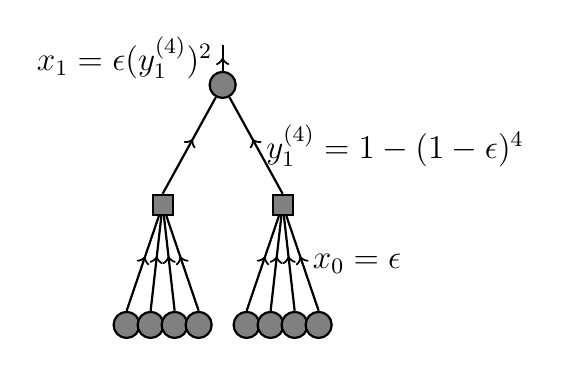
\begin{tikzpicture}
\def \depth{0.6in}; %vertical gap between nodes/levels
\def \gap{0.3in}; %Horizontal gap between nodes
\def \gapA{0.12in}; %Encoder Width
\def \gapB{0.12in}; %Encoder Width
\def \textoffs{0.18in}; %Offset for writing text above a node
\def\nodewidth{0.1in};
\tikzstyle{check} = [rectangle, draw, text centered, thick, fill=gray,
                          minimum height=\nodewidth, minimum width=\nodewidth]
\tikzstyle{bit} = [circle, draw, text centered, thick, fill=gray,
                          radius=0.5*\nodewidth]
                          
\def \fsize{\large}; %Defining a generic font size to be adjusted depending on the scaling
\def \dotsize{\Huge}; %Defining a generic font size to be adjusted depending on the scaling


\node [bit](b1) at (0,0) {} ;
\begin{scope}[thick,decoration={
    markings,
    mark=at position 0.5 with {\arrow{>}}}
    ] 
\draw[postaction={decorate}](b1)--+(0,0.2in)node[midway,left]{\fsize{$x_{1}=\epsilon (y_1^{(4)})^2$}};
\end{scope}
%Level 2
\node[check] (c21) at ([xshift=-\gap,yshift=-\depth]b1) {};
\node[check] (c22) at ([xshift=+\gap,yshift=-\depth]b1) {};

%Lines form level 1-level 2
\begin{scope}[thick,decoration={
    markings,
    mark=at position 0.5 with {\arrow{<}}}
    ] 
\draw[postaction={decorate}](b1)--(c21.north);
\draw[postaction={decorate}](b1)--(c22.north)node[midway,right,align=left]{\fsize{$y_{1}^{(4)}=1-(1-\epsilon)^4$}};
%\draw[postaction={decorate}](b1)--(c22.north)node[midway,right,align=left]{\fsize{$y_{1}^{(4)}=$} \\ \fsize{ $1-(1-\epsilon)^4$}};
\end{scope}

%Level 3
\node[bit] (b31) at ([xshift=-0.18in,yshift=-\depth]c21) {};
\node[bit] (b32) at ([xshift=-0.06in,yshift=-\depth]c21) {};
\node[bit] (b33) at ([xshift=+0.06in,yshift=-\depth]c21) {};
\node[bit] (b34) at ([xshift=+0.18in,yshift=-\depth]c21) {};
\node[bit] (b35) at ([xshift=-0.18in,yshift=-\depth]c22) {};
\node[bit] (b36) at ([xshift=-0.06in,yshift=-\depth]c22) {};
\node[bit] (b37) at ([xshift=+0.06in,yshift=-\depth]c22) {};
\node[bit] (b38) at ([xshift=+0.18in,yshift=-\depth]c22) {};

%Lines form level 2-level 3


\begin{scope}[thick, decoration={
    markings,
    mark=at position 0.5 with {\arrow{<}}}
    ] 
\draw[postaction={decorate}](c21)--(b31.north);
\draw[postaction={decorate}](c21)--(b32.north);
\draw[postaction={decorate}](c21)--(b33.north); 
\draw[postaction={decorate}](c21)--(b34.north);
\draw[postaction={decorate}](c22)--(b35.north);
\draw[postaction={decorate}](c22)--(b36.north); 
\draw[postaction={decorate}](c22)--(b37.north);
\draw[postaction={decorate}](c22)--(b38.north)node[midway,right]{\fsize{$x_{0}=\epsilon$}};
    \end{scope}




\end{tikzpicture}}
\\ \scriptsize{$P(T)=\rho_5^2$}
%\\ \scriptsize{$P(T\in\mathcal{T}_1(\lambda,\rho))=\rho_5^2$}
\end{center}
\end{column}
}
\end{columns}
\only<4->{
\begin{block}{}
\begin{eqnarray*}
\mathbb{E}_{\text{LDPC}(\lambda,\rho)}[x_1]&=&\sum\limits_{T\in\mathcal{T}_{1}(\lambda,\rho)}P(T)*x_1(T,\epsilon)\\
&=&\epsilon(\rho_4 y_1^{(3)}+\rho_5 y_1^{(4)})^2\\
&=&\epsilon(1-\rho_4 (1-\epsilon)^{3}-\rho_5 (1-\epsilon)^{4})^2\\
&=&\epsilon\lambda\left(1-\rho(1-\epsilon)\right)
%&=&\epsilon(1-\rho(1-\epsilon))^2\\
\end{eqnarray*}
\end{block}
}
\end{frame}
%--------------------------------------------------------------------------------------
\begin{frame}{Threshold}
%\begin{block}{Convergence condition}
%%\begin{eqnarray*}
%%  x_0 &=& \epsilon \\
%%  y_l &=& 1-\rho(1-x_l) \\
%%  x_l &=& \epsilon \lambda(y_{l-1}) \\
%%  x_l &=& \epsilon \lambda(1-\rho(1-x_{l-1})) = f(\epsilon,x_{l-1})
%%\end{eqnarray*}
%
%\end{block}
\vspace{-2mm}
\begin{block}{Convergence condition}
\[ x_l  = \epsilon \lambda(1-\rho(1-x_{l-1})) = f(\epsilon,x_{l-1}) \]
\[
\begin{array}{rl}
\text{$x_l$ converges to 0 if} & f(\epsilon,x) < x, \ x \in (0,\epsilon] \\
\text{There is a fixed point if} & f(\epsilon,x) = x, \ \text{for some} \ x \in (0,\epsilon]
\end{array}
\]
\end{block}
\pause
\begin{center}
  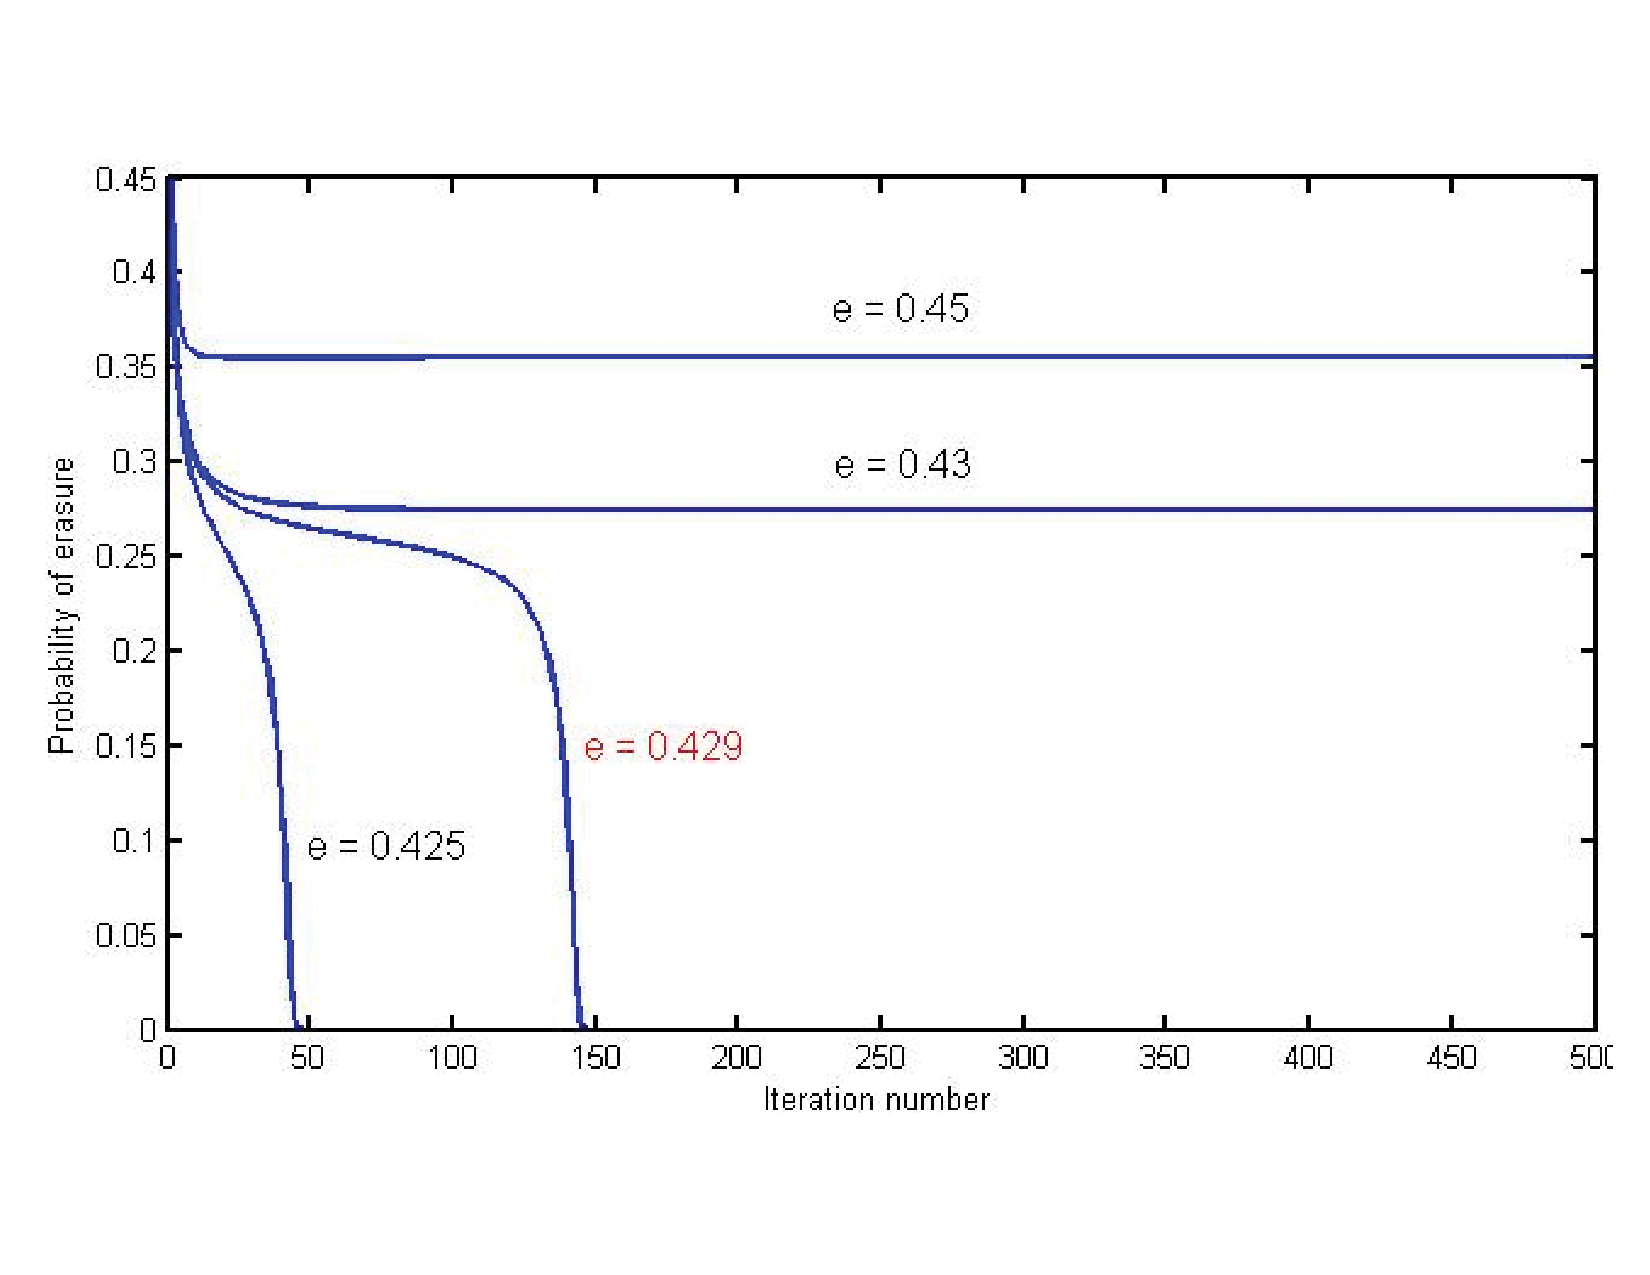
\includegraphics[width=2.5in]{DE36sim}
\end{center}
\pause
\vspace*{-3mm}
\begin{block}{The threshold $\epsilon^{\text{BP}}(\lambda,\rho)$ is defined as}
\[
\epsilon^{\text{BP}}(\lambda,\rho) = \sup \{\epsilon \in [0,1]: x_l \rightarrow 0 \ \text{as} \ l \rightarrow \infty \}
\]
\end{block}

\end{frame}
%--------------------------------------------------------------------------------------
\begin{frame}{Exit charts - Ashikmin, Kramer, ten Brink'04}
\begin{block}{Node functions}
\begin{itemize}
\item Var node function: $v_{\epsilon}(x) = \epsilon \lambda(x)$
\item Check node function: $c(x) = 1- \rho(1-x)$
\end{itemize}
\end{block}
\begin{columns}
\begin{column}{0.47\textwidth}
\begin{center}
\scalebox{0.35}{% This file was created by matlab2tikz v0.4.7 running on MATLAB 7.14.
% Copyright (c) 2008--2014, Nico Schlömer <nico.schloemer@gmail.com>
% All rights reserved.
% Minimal pgfplots version: 1.3
% 
% The latest updates can be retrieved from
%   http://www.mathworks.com/matlabcentral/fileexchange/22022-matlab2tikz
% where you can also make suggestions and rate matlab2tikz.
% 
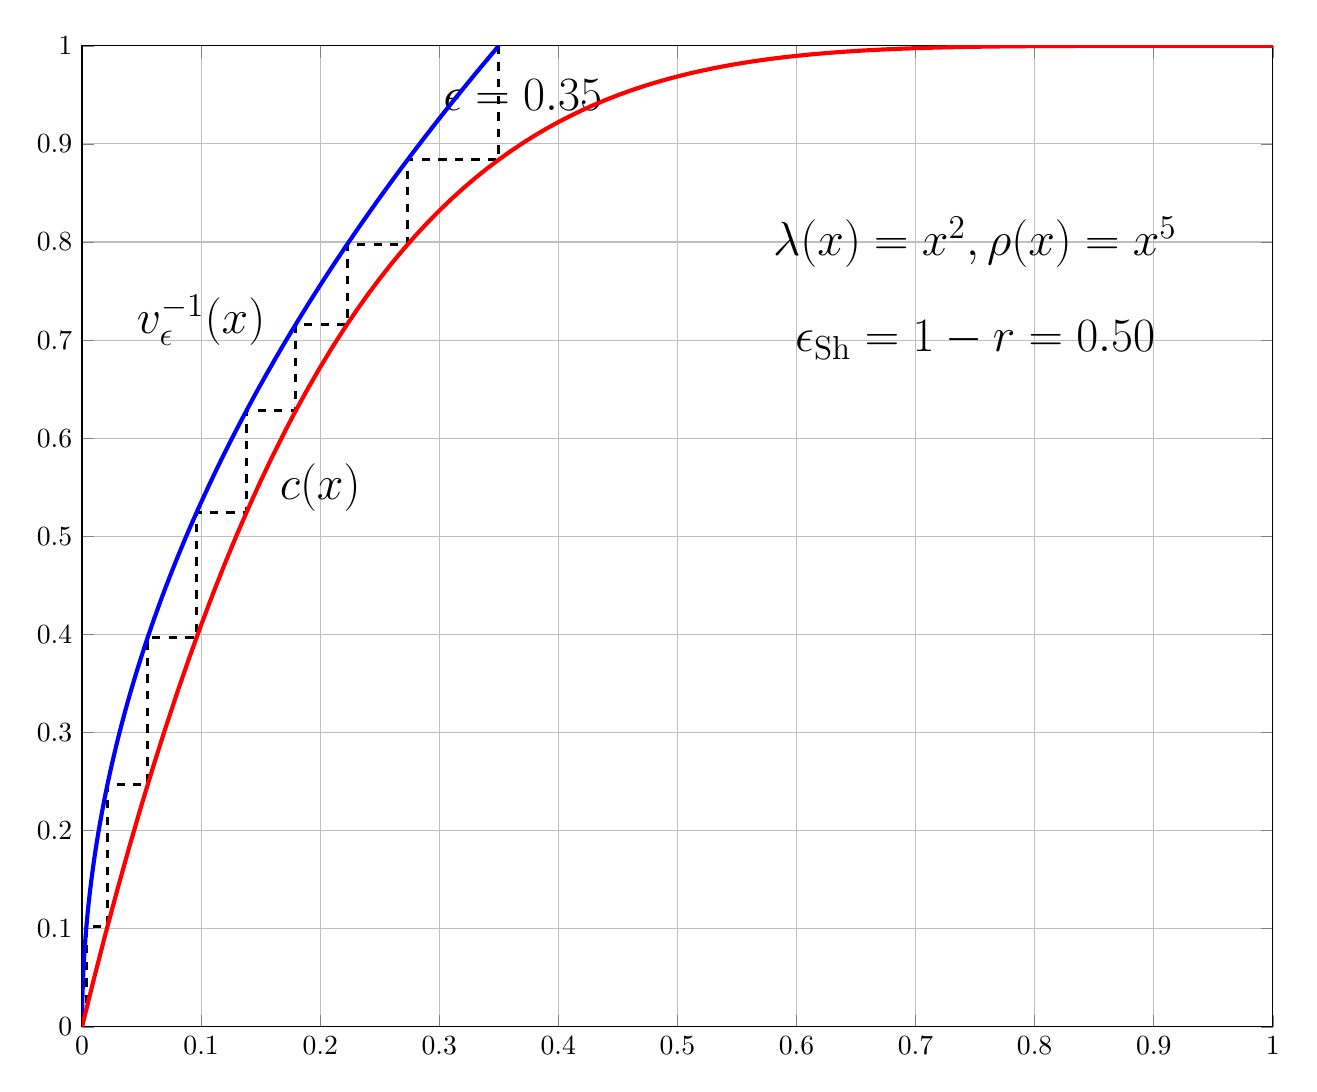
\begin{tikzpicture}
\def\fsize{\LARGE}
\begin{axis}[%
width=5.95380358705162in,
height=4.90490244969379in,
scale only axis,
xmin=0,
xmax=1,
xmajorgrids,
ymin=0,
ymax=1,
ymajorgrids
]
\node at (axis cs:0.2,0.55) {\fsize{$c(x)$}};
\node at (axis cs:0.1,0.72) {\fsize{$v_{\epsilon}^{-1}(x)$}};
\node at (axis cs:0.37,0.95) {\fsize{$\epsilon=0.35$}};

\node at (axis cs:0.75,0.8){\fsize{$\lambda(x)=x^2,\rho(x)=x^{5}$}};%\sum_{i=1}^{N}\binom{\alpha}{i}(-1)^{i-1}x^i$}};
\node at (axis cs:0.75,0.7){\fsize{$\epsilon_{\text{Sh}}=1-r=0.50 $}};
%\node at (axis cs:0.75,0.8){\fsize{$\rho(x)=x^{10},\alpha=0.1,N=50.$}};



\addplot [color=black,dashed,line width=1.0pt]
  table[row sep=crcr]{0.35	1\\
0.350000  0.883971 \\ 
0.273492  0.883971 \\ 
0.273492  0.797603 \\ 
0.222660  0.797603 \\ 
0.222660  0.716172 \\ 
0.179516  0.716172 \\ 
0.179516  0.628164 \\ 
0.138107  0.628164 \\ 
0.138107  0.524372 \\ 
0.096238  0.524372 \\ 
0.096238  0.397065 \\ 
0.055181  0.397065 \\ 
0.055181  0.247091 \\ 
0.021369  0.247091 \\ 
0.021369  0.102375 \\ 
0.003668  0.102375 \\ 
0.003668  0.018207 \\ 
0.000116  0.018207 \\ 
0.000116  0.000580 \\ 
0.000000  0.000580 \\ 
};
  
\addplot [color=blue,solid,line width=1.5pt]
  table[row sep=crcr]{0	0\\
3.5e-05	0.01\\
0.00014	0.02\\
0.000315	0.03\\
0.00056	0.04\\
0.000875	0.05\\
0.00126	0.06\\
0.001715	0.07\\
0.00224	0.08\\
0.002835	0.09\\
0.0035	0.1\\
0.004235	0.11\\
0.00504	0.12\\
0.005915	0.13\\
0.00686	0.14\\
0.007875	0.15\\
0.00896	0.16\\
0.010115	0.17\\
0.01134	0.18\\
0.012635	0.19\\
0.014	0.2\\
0.015435	0.21\\
0.01694	0.22\\
0.018515	0.23\\
0.02016	0.24\\
0.021875	0.25\\
0.02366	0.26\\
0.025515	0.27\\
0.02744	0.28\\
0.029435	0.29\\
0.0315	0.3\\
0.033635	0.31\\
0.03584	0.32\\
0.038115	0.33\\
0.04046	0.34\\
0.042875	0.35\\
0.04536	0.36\\
0.047915	0.37\\
0.05054	0.38\\
0.053235	0.39\\
0.056	0.4\\
0.058835	0.41\\
0.06174	0.42\\
0.064715	0.43\\
0.06776	0.44\\
0.070875	0.45\\
0.07406	0.46\\
0.077315	0.47\\
0.08064	0.48\\
0.084035	0.49\\
0.0875	0.5\\
0.091035	0.51\\
0.09464	0.52\\
0.098315	0.53\\
0.10206	0.54\\
0.105875	0.55\\
0.10976	0.56\\
0.113715	0.57\\
0.11774	0.58\\
0.121835	0.59\\
0.126	0.6\\
0.130235	0.61\\
0.13454	0.62\\
0.138915	0.63\\
0.14336	0.64\\
0.147875	0.65\\
0.15246	0.66\\
0.157115	0.67\\
0.16184	0.68\\
0.166635	0.69\\
0.1715	0.7\\
0.176435	0.71\\
0.18144	0.72\\
0.186515	0.73\\
0.19166	0.74\\
0.196875	0.75\\
0.20216	0.76\\
0.207515	0.77\\
0.21294	0.78\\
0.218435	0.79\\
0.224	0.8\\
0.229635	0.81\\
0.23534	0.82\\
0.241115	0.83\\
0.24696	0.84\\
0.252875	0.85\\
0.25886	0.86\\
0.264915	0.87\\
0.27104	0.88\\
0.277235	0.89\\
0.2835	0.9\\
0.289835	0.91\\
0.29624	0.92\\
0.302715	0.93\\
0.30926	0.94\\
0.315875	0.95\\
0.32256	0.96\\
0.329315	0.97\\
0.33614	0.98\\
0.343035	0.99\\
0.35	1\\
};
\addplot [color=red,solid,line width=1.5pt]
  table[row sep=crcr]{0	0\\
0.01	0.0490099501000001\\
0.02	0.0960792032000002\\
0.03	0.1412659743\\
0.04	0.1846273024\\
0.05	0.2262190625\\
0.06	0.2660959776\\
0.07	0.3043116307\\
0.08	0.3409184768\\
0.09	0.3759678549\\
0.1	0.40951\\
0.11	0.4415940551\\
0.12	0.4722680832\\
0.13	0.5015790793\\
0.14	0.5295729824\\
0.15	0.5562946875\\
0.16	0.5817880576\\
0.17	0.6060959357\\
0.18	0.6292601568\\
0.19	0.6513215599\\
0.2	0.67232\\
0.21	0.6922943601\\
0.22	0.7112825632\\
0.23	0.7293215843\\
0.24	0.7464474624\\
0.25	0.7626953125\\
0.26	0.7780993376\\
0.27	0.7926928407\\
0.28	0.8065082368\\
0.29	0.8195770649\\
0.3	0.83193\\
0.31	0.8435968651\\
0.32	0.8546066432\\
0.33	0.8649874893\\
0.34	0.8747667424\\
0.35	0.8839709375\\
0.36	0.8926258176\\
0.37	0.9007563457\\
0.38	0.9083867168\\
0.39	0.9155403699\\
0.4	0.92224\\
0.41	0.9285075701\\
0.42	0.9343643232\\
0.43	0.9398307943\\
0.44	0.9449268224\\
0.45	0.9496715625\\
0.46	0.9540834976\\
0.47	0.9581804507\\
0.48	0.9619795968\\
0.49	0.9654974749\\
0.5	0.96875\\
0.51	0.9717524751\\
0.52	0.9745196032\\
0.53	0.9770654993\\
0.54	0.9794037024\\
0.55	0.9815471875\\
0.56	0.9835083776\\
0.57	0.9852991557\\
0.58	0.9869308768\\
0.59	0.9884143799\\
0.6	0.98976\\
0.61	0.9909775801\\
0.62	0.9920764832\\
0.63	0.9930656043\\
0.64	0.9939533824\\
0.65	0.9947478125\\
0.66	0.9954564576\\
0.67	0.9960864607\\
0.68	0.9966445568\\
0.69	0.9971370849\\
0.7	0.99757\\
0.71	0.9979488851\\
0.72	0.9982789632\\
0.73	0.9985651093\\
0.74	0.9988118624\\
0.75	0.9990234375\\
0.76	0.9992037376\\
0.77	0.9993563657\\
0.78	0.9994846368\\
0.79	0.9995915899\\
0.8	0.99968\\
0.81	0.9997523901\\
0.82	0.9998110432\\
0.83	0.9998580143\\
0.84	0.9998951424\\
0.85	0.9999240625\\
0.86	0.9999462176\\
0.87	0.9999628707\\
0.88	0.9999751168\\
0.89	0.9999838949\\
0.9	0.99999\\
0.91	0.9999940951\\
0.92	0.9999967232\\
0.93	0.9999983193\\
0.94	0.9999992224\\
0.95	0.9999996875\\
0.96	0.9999998976\\
0.97	0.9999999757\\
0.98	0.9999999968\\
0.99	0.9999999999\\
1	1\\
};
\end{axis}
\end{tikzpicture}%}
\end{center}
\end{column}

\begin{column}{0.47\textwidth}
\begin{center}
\scalebox{0.35}{% This file was created by matlab2tikz v0.4.7 running on MATLAB 7.14.
% Copyright (c) 2008--2014, Nico Schlömer <nico.schloemer@gmail.com>
% All rights reserved.
% Minimal pgfplots version: 1.3
% 
% The latest updates can be retrieved from
%   http://www.mathworks.com/matlabcentral/fileexchange/22022-matlab2tikz
% where you can also make suggestions and rate matlab2tikz.
% 
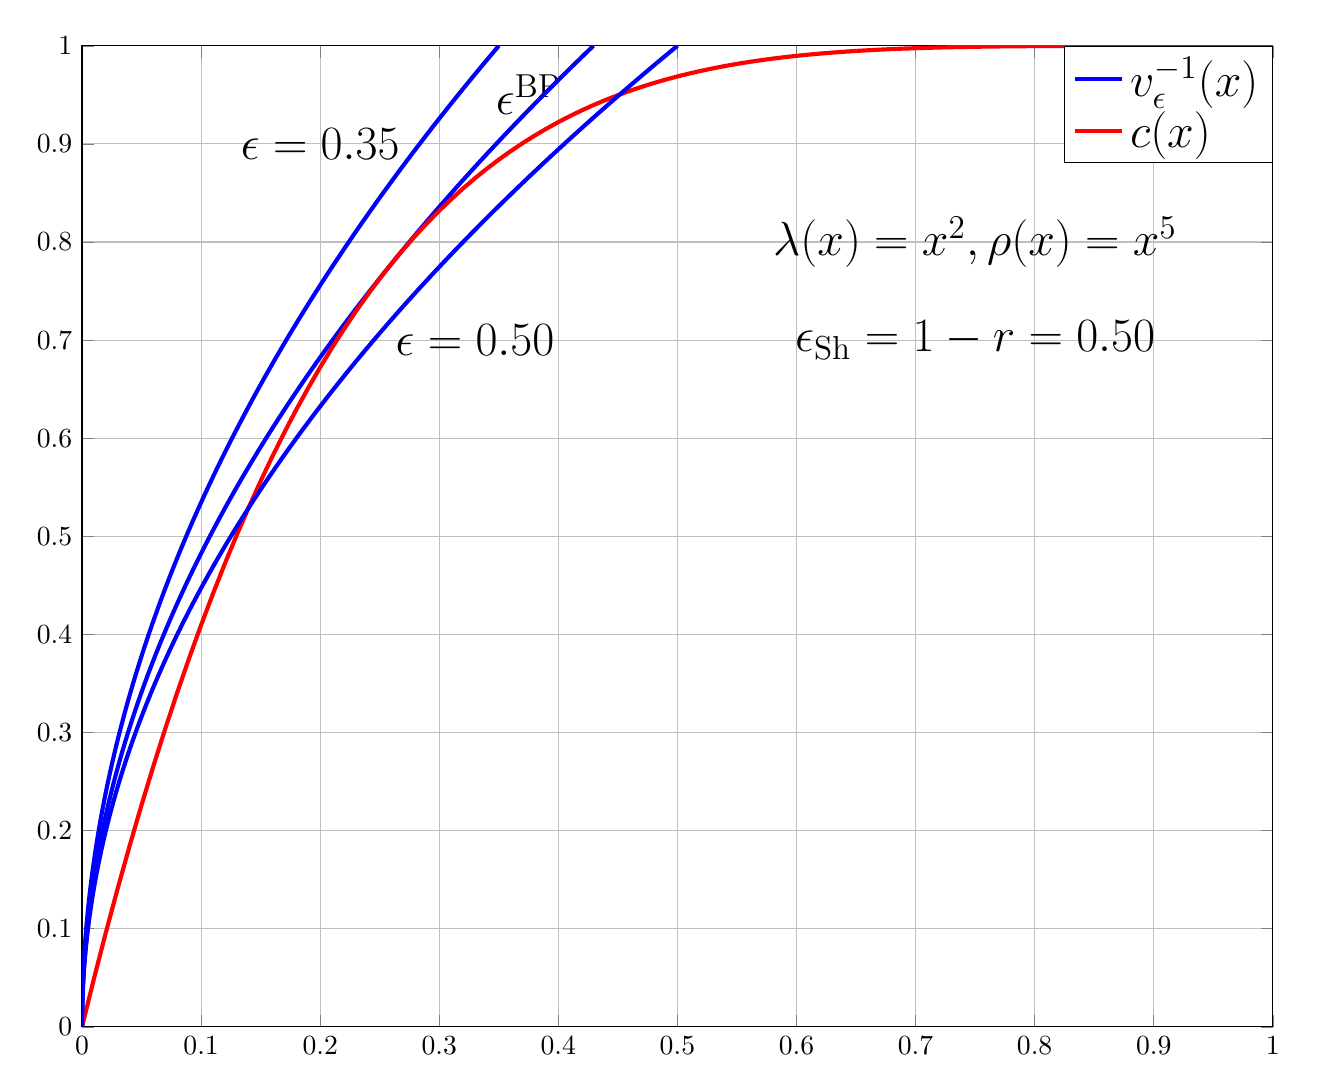
\begin{tikzpicture}
\def\fsize{\LARGE}
\begin{axis}[%
width=5.95380358705162in,
height=4.90490244969379in,
scale only axis,
xmin=0,
xmax=1,
xmajorgrids,
ymin=0,
ymax=1,
legend style={at={(1,1)},anchor=north east,draw=black,fill=white,legend cell align=left,font=\LARGE},
ymajorgrids
]
\node at (axis cs:0.33,0.7){\LARGE{$\epsilon=0.50$}};
\node at (axis cs:0.2,0.9){\LARGE{$\epsilon=0.35$}};
\node at (axis cs:0.375,0.95){\LARGE{$\epsilon^{\text{BP}}$}};

\node at (axis cs:0.75,0.8){\fsize{$\lambda(x)=x^2,\rho(x)=x^{5}$}};%\sum_{i=1}^{N}\binom{\alpha}{i}(-1)^{i-1}x^i$}};
\node at (axis cs:0.75,0.7){\fsize{$\epsilon_{\text{Sh}}=1-r=0.50 $}};

\addlegendentry{\LARGE{$v_{\epsilon}^{-1}(x)$}};
\addplot [color=blue,solid,line width=1.5pt]
  table[row sep=crcr]{0	0\\
4.2944e-05	0.01\\
0.000171776	0.02\\
0.000386496	0.03\\
0.000687104	0.04\\
0.0010736	0.05\\
0.001545984	0.06\\
0.002104256	0.07\\
0.002748416	0.08\\
0.003478464	0.09\\
0.0042944	0.1\\
0.005196224	0.11\\
0.006183936	0.12\\
0.007257536	0.13\\
0.008417024	0.14\\
0.0096624	0.15\\
0.010993664	0.16\\
0.012410816	0.17\\
0.013913856	0.18\\
0.015502784	0.19\\
0.0171776	0.2\\
0.018938304	0.21\\
0.020784896	0.22\\
0.022717376	0.23\\
0.024735744	0.24\\
0.02684	0.25\\
0.029030144	0.26\\
0.031306176	0.27\\
0.033668096	0.28\\
0.036115904	0.29\\
0.0386496	0.3\\
0.041269184	0.31\\
0.043974656	0.32\\
0.046766016	0.33\\
0.049643264	0.34\\
0.0526064	0.35\\
0.055655424	0.36\\
0.058790336	0.37\\
0.062011136	0.38\\
0.065317824	0.39\\
0.0687104	0.4\\
0.072188864	0.41\\
0.075753216	0.42\\
0.079403456	0.43\\
0.083139584	0.44\\
0.0869616	0.45\\
0.090869504	0.46\\
0.094863296	0.47\\
0.098942976	0.48\\
0.103108544	0.49\\
0.10736	0.5\\
0.111697344	0.51\\
0.116120576	0.52\\
0.120629696	0.53\\
0.125224704	0.54\\
0.1299056	0.55\\
0.134672384	0.56\\
0.139525056	0.57\\
0.144463616	0.58\\
0.149488064	0.59\\
0.1545984	0.6\\
0.159794624	0.61\\
0.165076736	0.62\\
0.170444736	0.63\\
0.175898624	0.64\\
0.1814384	0.65\\
0.187064064	0.66\\
0.192775616	0.67\\
0.198573056	0.68\\
0.204456384	0.69\\
0.2104256	0.7\\
0.216480704	0.71\\
0.222621696	0.72\\
0.228848576	0.73\\
0.235161344	0.74\\
0.24156	0.75\\
0.248044544	0.76\\
0.254614976	0.77\\
0.261271296	0.78\\
0.268013504	0.79\\
0.2748416	0.8\\
0.281755584	0.81\\
0.288755456	0.82\\
0.295841216	0.83\\
0.303012864	0.84\\
0.3102704	0.85\\
0.317613824	0.86\\
0.325043136	0.87\\
0.332558336	0.88\\
0.340159424	0.89\\
0.3478464	0.9\\
0.355619264	0.91\\
0.363478016	0.92\\
0.371422656	0.93\\
0.379453184	0.94\\
0.3875696	0.95\\
0.395771904	0.96\\
0.404060096	0.97\\
0.412434176	0.98\\
0.420894144	0.99\\
0.42944	1\\
};

\addlegendentry{\LARGE{$c(x)$}};
\addplot [color=red,solid,line width=1.5pt]
  table[row sep=crcr]{0	0\\
0.01	0.0490099501000001\\
0.02	0.0960792032000002\\
0.03	0.1412659743\\
0.04	0.1846273024\\
0.05	0.2262190625\\
0.06	0.2660959776\\
0.07	0.3043116307\\
0.08	0.3409184768\\
0.09	0.3759678549\\
0.1	0.40951\\
0.11	0.4415940551\\
0.12	0.4722680832\\
0.13	0.5015790793\\
0.14	0.5295729824\\
0.15	0.5562946875\\
0.16	0.5817880576\\
0.17	0.6060959357\\
0.18	0.6292601568\\
0.19	0.6513215599\\
0.2	0.67232\\
0.21	0.6922943601\\
0.22	0.7112825632\\
0.23	0.7293215843\\
0.24	0.7464474624\\
0.25	0.7626953125\\
0.26	0.7780993376\\
0.27	0.7926928407\\
0.28	0.8065082368\\
0.29	0.8195770649\\
0.3	0.83193\\
0.31	0.8435968651\\
0.32	0.8546066432\\
0.33	0.8649874893\\
0.34	0.8747667424\\
0.35	0.8839709375\\
0.36	0.8926258176\\
0.37	0.9007563457\\
0.38	0.9083867168\\
0.39	0.9155403699\\
0.4	0.92224\\
0.41	0.9285075701\\
0.42	0.9343643232\\
0.43	0.9398307943\\
0.44	0.9449268224\\
0.45	0.9496715625\\
0.46	0.9540834976\\
0.47	0.9581804507\\
0.48	0.9619795968\\
0.49	0.9654974749\\
0.5	0.96875\\
0.51	0.9717524751\\
0.52	0.9745196032\\
0.53	0.9770654993\\
0.54	0.9794037024\\
0.55	0.9815471875\\
0.56	0.9835083776\\
0.57	0.9852991557\\
0.58	0.9869308768\\
0.59	0.9884143799\\
0.6	0.98976\\
0.61	0.9909775801\\
0.62	0.9920764832\\
0.63	0.9930656043\\
0.64	0.9939533824\\
0.65	0.9947478125\\
0.66	0.9954564576\\
0.67	0.9960864607\\
0.68	0.9966445568\\
0.69	0.9971370849\\
0.7	0.99757\\
0.71	0.9979488851\\
0.72	0.9982789632\\
0.73	0.9985651093\\
0.74	0.9988118624\\
0.75	0.9990234375\\
0.76	0.9992037376\\
0.77	0.9993563657\\
0.78	0.9994846368\\
0.79	0.9995915899\\
0.8	0.99968\\
0.81	0.9997523901\\
0.82	0.9998110432\\
0.83	0.9998580143\\
0.84	0.9998951424\\
0.85	0.9999240625\\
0.86	0.9999462176\\
0.87	0.9999628707\\
0.88	0.9999751168\\
0.89	0.9999838949\\
0.9	0.99999\\
0.91	0.9999940951\\
0.92	0.9999967232\\
0.93	0.9999983193\\
0.94	0.9999992224\\
0.95	0.9999996875\\
0.96	0.9999998976\\
0.97	0.9999999757\\
0.98	0.9999999968\\
0.99	0.9999999999\\
1	1\\
};

\addplot [color=blue,solid,line width=1.5pt]
  table[row sep=crcr]{0	0\\
3.5e-05	0.01\\
0.00014	0.02\\
0.000315	0.03\\
0.00056	0.04\\
0.000875	0.05\\
0.00126	0.06\\
0.001715	0.07\\
0.00224	0.08\\
0.002835	0.09\\
0.0035	0.1\\
0.004235	0.11\\
0.00504	0.12\\
0.005915	0.13\\
0.00686	0.14\\
0.007875	0.15\\
0.00896	0.16\\
0.010115	0.17\\
0.01134	0.18\\
0.012635	0.19\\
0.014	0.2\\
0.015435	0.21\\
0.01694	0.22\\
0.018515	0.23\\
0.02016	0.24\\
0.021875	0.25\\
0.02366	0.26\\
0.025515	0.27\\
0.02744	0.28\\
0.029435	0.29\\
0.0315	0.3\\
0.033635	0.31\\
0.03584	0.32\\
0.038115	0.33\\
0.04046	0.34\\
0.042875	0.35\\
0.04536	0.36\\
0.047915	0.37\\
0.05054	0.38\\
0.053235	0.39\\
0.056	0.4\\
0.058835	0.41\\
0.06174	0.42\\
0.064715	0.43\\
0.06776	0.44\\
0.070875	0.45\\
0.07406	0.46\\
0.077315	0.47\\
0.08064	0.48\\
0.084035	0.49\\
0.0875	0.5\\
0.091035	0.51\\
0.09464	0.52\\
0.098315	0.53\\
0.10206	0.54\\
0.105875	0.55\\
0.10976	0.56\\
0.113715	0.57\\
0.11774	0.58\\
0.121835	0.59\\
0.126	0.6\\
0.130235	0.61\\
0.13454	0.62\\
0.138915	0.63\\
0.14336	0.64\\
0.147875	0.65\\
0.15246	0.66\\
0.157115	0.67\\
0.16184	0.68\\
0.166635	0.69\\
0.1715	0.7\\
0.176435	0.71\\
0.18144	0.72\\
0.186515	0.73\\
0.19166	0.74\\
0.196875	0.75\\
0.20216	0.76\\
0.207515	0.77\\
0.21294	0.78\\
0.218435	0.79\\
0.224	0.8\\
0.229635	0.81\\
0.23534	0.82\\
0.241115	0.83\\
0.24696	0.84\\
0.252875	0.85\\
0.25886	0.86\\
0.264915	0.87\\
0.27104	0.88\\
0.277235	0.89\\
0.2835	0.9\\
0.289835	0.91\\
0.29624	0.92\\
0.302715	0.93\\
0.30926	0.94\\
0.315875	0.95\\
0.32256	0.96\\
0.329315	0.97\\
0.33614	0.98\\
0.343035	0.99\\
0.35	1\\
};

\addplot [color=blue,solid,line width=1.5pt]
  table[row sep=crcr]{0	0\\
5e-05	0.01\\
0.0002	0.02\\
0.00045	0.03\\
0.0008	0.04\\
0.00125	0.05\\
0.0018	0.06\\
0.00245	0.07\\
0.0032	0.08\\
0.00405	0.09\\
0.005	0.1\\
0.00605	0.11\\
0.0072	0.12\\
0.00845	0.13\\
0.0098	0.14\\
0.01125	0.15\\
0.0128	0.16\\
0.01445	0.17\\
0.0162	0.18\\
0.01805	0.19\\
0.02	0.2\\
0.02205	0.21\\
0.0242	0.22\\
0.02645	0.23\\
0.0288	0.24\\
0.03125	0.25\\
0.0338	0.26\\
0.03645	0.27\\
0.0392	0.28\\
0.04205	0.29\\
0.045	0.3\\
0.04805	0.31\\
0.0512	0.32\\
0.05445	0.33\\
0.0578	0.34\\
0.06125	0.35\\
0.0648	0.36\\
0.06845	0.37\\
0.0722	0.38\\
0.07605	0.39\\
0.08	0.4\\
0.08405	0.41\\
0.0882	0.42\\
0.09245	0.43\\
0.0968	0.44\\
0.10125	0.45\\
0.1058	0.46\\
0.11045	0.47\\
0.1152	0.48\\
0.12005	0.49\\
0.125	0.5\\
0.13005	0.51\\
0.1352	0.52\\
0.14045	0.53\\
0.1458	0.54\\
0.15125	0.55\\
0.1568	0.56\\
0.16245	0.57\\
0.1682	0.58\\
0.17405	0.59\\
0.18	0.6\\
0.18605	0.61\\
0.1922	0.62\\
0.19845	0.63\\
0.2048	0.64\\
0.21125	0.65\\
0.2178	0.66\\
0.22445	0.67\\
0.2312	0.68\\
0.23805	0.69\\
0.245	0.7\\
0.25205	0.71\\
0.2592	0.72\\
0.26645	0.73\\
0.2738	0.74\\
0.28125	0.75\\
0.2888	0.76\\
0.29645	0.77\\
0.3042	0.78\\
0.31205	0.79\\
0.32	0.8\\
0.32805	0.81\\
0.3362	0.82\\
0.34445	0.83\\
0.3528	0.84\\
0.36125	0.85\\
0.3698	0.86\\
0.37845	0.87\\
0.3872	0.88\\
0.39605	0.89\\
0.405	0.9\\
0.41405	0.91\\
0.4232	0.92\\
0.43245	0.93\\
0.4418	0.94\\
0.45125	0.95\\
0.4608	0.96\\
0.47045	0.97\\
0.4802	0.98\\
0.49005	0.99\\
0.5	1\\
};
\end{axis}
\end{tikzpicture}%}
\end{center}

\end{column}

\end{columns}
\end{frame}
%--------------------------------------------------------------------------------------
\begin{frame}{Optimality of EXIT chart matching}
\begin{itemize}
\item Var node function: $v_{\epsilon}(x) = \epsilon \lambda(x)$
\item Check node function: $c(x) = 1- \rho(1-x)$
\end{itemize}
\begin{center}
\scalebox{0.45}{% This file was created by matlab2tikz v0.4.7 running on MATLAB 7.14.
% Copyright (c) 2008--2014, Nico Schlömer <nico.schloemer@gmail.com>
% All rights reserved.
% Minimal pgfplots version: 1.3
% 
% The latest updates can be retrieved from
%   http://www.mathworks.com/matlabcentral/fileexchange/22022-matlab2tikz
% where you can also make suggestions and rate matlab2tikz.
% 
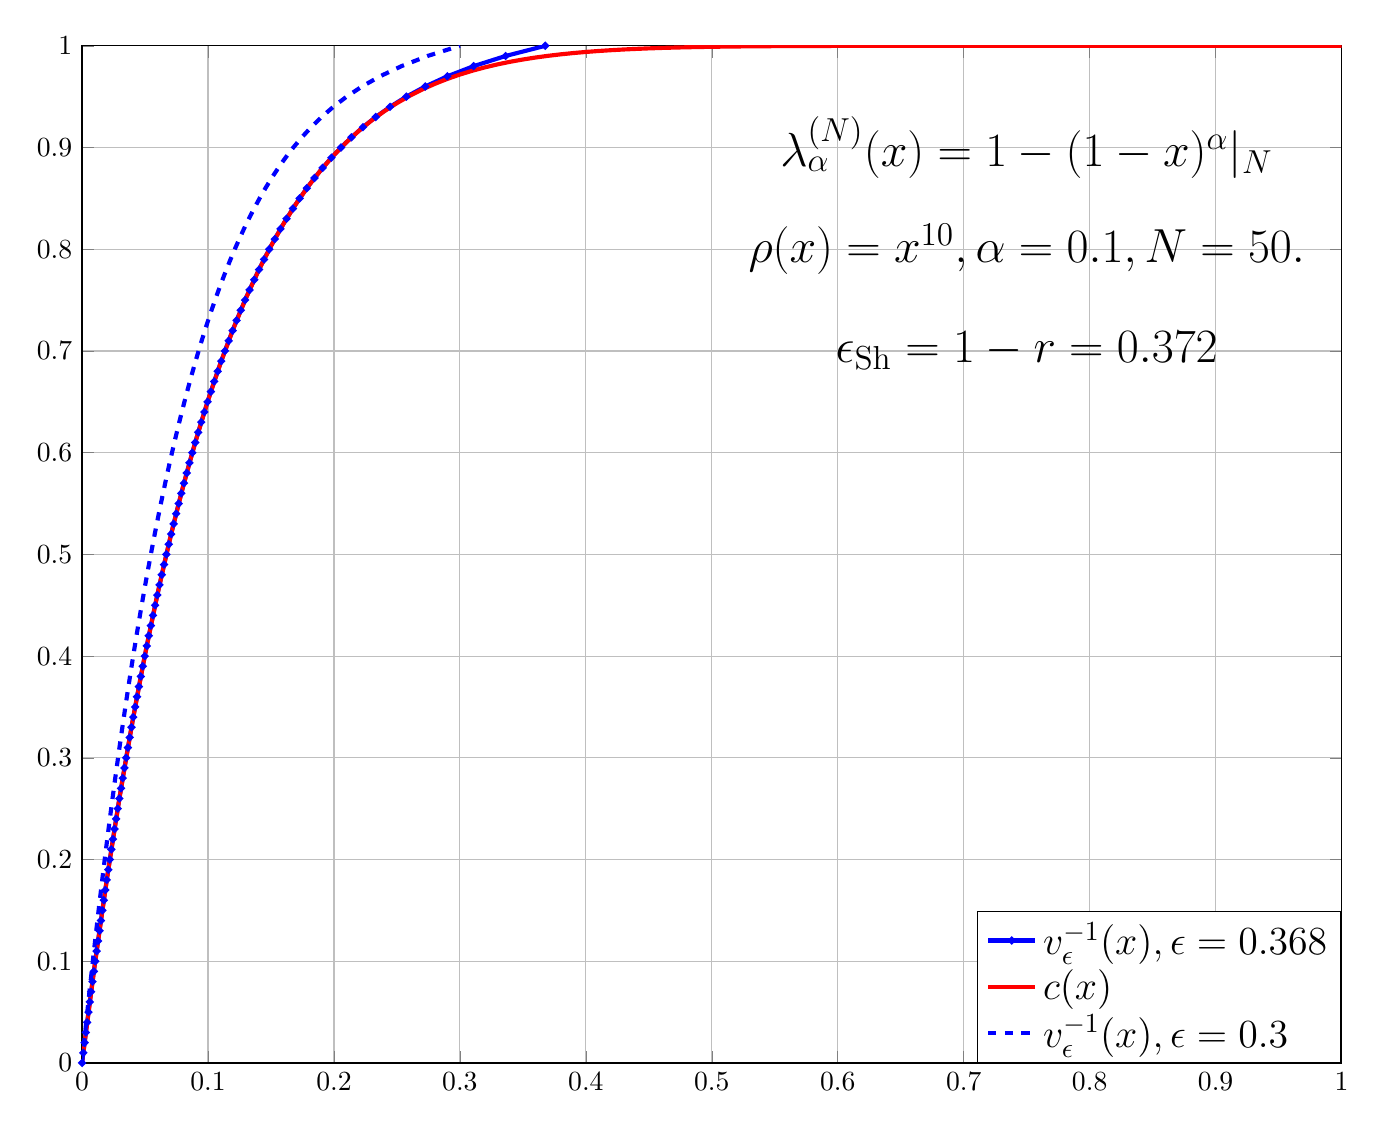
\begin{tikzpicture}
\def \fsize{\LARGE}
\begin{axis}[%
width=6.29770559930009in,
height=5.08572834645669in,
scale only axis,
xmin=0,
xmax=1,
xmajorgrids,
ymin=0,
ymax=1,
legend style={at={(1,0)},anchor=south east,draw=black,fill=white,legend cell align=left,font=\fsize},
ymajorgrids
]

\node at (axis cs:0.75,0.9){\fsize{$\lambda_{\alpha}^{(N)}(x)=1-(1-x)^{\alpha}|_{N}$}};%\sum_{i=1}^{N}\binom{\alpha}{i}(-1)^{i-1}x^i$}};
\node at (axis cs:0.75,0.8){\fsize{$\rho(x)=x^{10},\alpha=0.1,N=50.$}};
\node at (axis cs:0.75,0.7){\fsize{$\epsilon_{\text{Sh}}=1-r=0.372 $}};


\addlegendentry{\Large{$v_{\epsilon}^{-1}(x),\epsilon=0.368$}};
\addplot [color=blue,mark=*,mark size=0.5pt,solid,line width=1.5pt]
  table[row sep=crcr]{0	0\\
0.00100452870824995	0.01\\
0.00201823135843042	0.02\\
0.0030412866381062	0.03\\
0.00407387860214938	0.04\\
0.0051161968918237	0.05\\
0.00616843696522343	0.06\\
0.00723080033978309	0.07\\
0.00830349484762741	0.08\\
0.00938673490458918	0.09\\
0.0104807417937856	0.1\\
0.0115857439647124	0.11\\
0.0127019773488898	0.12\\
0.0138296856931755	0.13\\
0.0149691209119498	0.14\\
0.0161205434594737	0.15\\
0.0172842227238285	0.16\\
0.0184604374439603	0.17\\
0.0196494761514822	0.18\\
0.0208516376390232	0.19\\
0.0220672314570715	0.2\\
0.0232965784414229	0.21\\
0.0245400112735353	0.22\\
0.0257978750762919	0.23\\
0.0270705280479034	0.24\\
0.0283583421369265	0.25\\
0.0296617037616551	0.26\\
0.0309810145774423	0.27\\
0.0323166922958518	0.28\\
0.0336691715599149	0.29\\
0.0350389048801824	0.3\\
0.0364263636367327	0.31\\
0.0378320391528112	0.32\\
0.0392564438463597	0.33\\
0.040700112466341	0.34\\
0.0421636034214935	0.35\\
0.043647500209963	0.36\\
0.0451524129591818	0.37\\
0.046678980086392	0.38\\
0.0482278700913825	0.39\\
0.0497997834943236	0.4\\
0.0513954549330765	0.41\\
0.0530156554360524	0.42\\
0.0546611948886202	0.43\\
0.0563329247132606	0.44\\
0.0580317407861738	0.45\\
0.0597585866159188	0.46\\
0.0615144568129612	0.47\\
0.0633004008827987	0.48\\
0.0651175273797047	0.49\\
0.0669670084631926	0.5\\
0.0688500849051623	0.51\\
0.0707680716025138	0.52\\
0.0727223636579612	0.53\\
0.0747144431010848	0.54\\
0.0767458863325731	0.55\\
0.0788183723874597	0.56\\
0.0809336921283443	0.57\\
0.0830937584975923	0.58\\
0.0853006179789351	0.59\\
0.0875564634445046	0.6\\
0.0898636485940515	0.61\\
0.0922247042301274	0.62\\
0.0946423566578192	0.63\\
0.0971195485521326	0.64\\
0.0996594627027419	0.65\\
0.102265549127682	0.66\\
0.104941556148684	0.67\\
0.10769156614654	0.68\\
0.110520036871966	0.69\\
0.113431849385121	0.7\\
0.116432363947291	0.71\\
0.119527485507556	0.72\\
0.122723740837558	0.73\\
0.126028369898529	0.74\\
0.129449434717698	0.75\\
0.132995949962507	0.76\\
0.13667804060955	0.77\\
0.14050713372094	0.78\\
0.144496193519323	0.79\\
0.148660011914131	0.8\\
0.153015570690002	0.81\\
0.157582497173504	0.82\\
0.162383642994294	0.83\\
0.167445826487868	0.84\\
0.172800794707139	0.85\\
0.17848648289442	0.86\\
0.184548680493846	0.87\\
0.191043257563369	0.88\\
0.198039169928183	0.89\\
0.205622554612463	0.9\\
0.213902362190138	0.91\\
0.22301816904284	0.92\\
0.233151098427202	0.93\\
0.244539196204305	0.94\\
0.257499215745708	0.95\\
0.272457655587535	0.96\\
0.289995192326096	0.97\\
0.310910548784957	0.98\\
0.336312608378763	0.99\\
0.367753630095884	1\\
};
\addlegendentry{\Large{$c(x)$}};
\addplot [color=red,solid,line width=1.5pt]
  table[row sep=crcr]{0	0\\
0.01	0.0956179249911957\\
0.02	0.182927193112453\\
0.03	0.262575873105072\\
0.04	0.335167364008499\\
0.05	0.401263060761621\\
0.06	0.461384885905101\\
0.07	0.516017692820707\\
0.08	0.565611545776368\\
0.09	0.610583881881892\\
0.1	0.6513215599\\
0.11	0.688182800700338\\
0.12	0.721499023990598\\
0.13	0.751576585808564\\
0.14	0.778698421111969\\
0.15	0.803125595659277\\
0.16	0.825098771234019\\
0.17	0.844839588127942\\
0.18	0.862551968664039\\
0.19	0.878423345409431\\
0.2	0.8926258176\\
0.21	0.905317239173732\\
0.22	0.916642241687638\\
0.23	0.926733195274138\\
0.24	0.935711110676601\\
0.25	0.943686485290527\\
0.26	0.950760096026441\\
0.27	0.957023741702964\\
0.28	0.962560937573755\\
0.29	0.967447564489901\\
0.3	0.9717524751\\
0.31	0.975538059393452\\
0.32	0.978860771798428\\
0.33	0.981771621954482\\
0.34	0.984316631190892\\
0.35	0.986537256655371\\
0.36	0.988470784953931\\
0.37	0.990150697081182\\
0.38	0.991607006341317\\
0.39	0.992866570883371\\
0.4	0.9939533824\\
0.41	0.994888832466994\\
0.42	0.995691957931006\\
0.43	0.996379666685431\\
0.44	0.996966945109039\\
0.45	0.997467048378809\\
0.46	0.997891674807351\\
0.47	0.998251125296345\\
0.48	0.998554448940509\\
0.49	0.998809575761724\\
0.5	0.9990234375\\
0.51	0.999202077337024\\
0.52	0.999350749378915\\
0.53	0.999474008677642\\
0.54	0.999575792525172\\
0.55	0.99965949371084\\
0.56	0.999728026390616\\
0.57	0.999783885176867\\
0.58	0.999829198018783\\
0.59	0.999865773406899\\
0.6	0.9998951424\\
0.61	0.999918595939148\\
0.62	0.99993721788152\\
0.63	0.999951914156276\\
0.64	0.999963438415599\\
0.65	0.999972414526465\\
0.66	0.999979356222459\\
0.67	0.999984684210147\\
0.68	0.999988741000932\\
0.69	0.99999180371713\\
0.7	0.9999940951\\
0.71	0.999995792927667\\
0.72	0.999997038032333\\
0.73	0.999997941088679\\
0.74	0.999998588329043\\
0.75	0.999999046325684\\
0.76	0.99999936596619\\
0.77	0.999999585734888\\
0.78	0.999999734400772\\
0.79	0.99999983320119\\
0.8	0.9999998976\\
0.81	0.999999938689337\\
0.82	0.999999964295328\\
0.83	0.999999979840061\\
0.84	0.999999989004884\\
0.85	0.999999994233496\\
0.86	0.999999997107453\\
0.87	0.999999998621415\\
0.88	0.999999999380826\\
0.89	0.999999999740626\\
0.9	0.9999999999\\
0.91	0.999999999965132\\
0.92	0.999999999989263\\
0.93	0.999999999997175\\
0.94	0.999999999999395\\
0.95	0.999999999999902\\
0.96	0.99999999999999\\
0.97	0.999999999999999\\
0.98	1\\
0.99	1\\
1	1\\
};
\addlegendentry{\Large{$v_{\epsilon}^{-1}(x),\epsilon=0.3$}};
\addplot [color=blue,dashed,line width=1.5pt]
  table[row sep=crcr]{0	0\\
0.000819457886510628	0.01\\
0.00164639954028805	0.02\\
0.00248097072813115	0.03\\
0.00332332159529237	0.04\\
0.00417360684419873	0.05\\
0.00503198592243547	0.06\\
0.00589862322057662	0.07\\
0.00677368828049021	0.08\\
0.00765735601479321	0.09\\
0.00854980693818275	0.1\\
0.00945122741142626	0.11\\
0.0103618098988538	0.12\\
0.0112817532402628	0.13\\
0.0122112629382179	0.14\\
0.0131505514618066	0.15\\
0.0140998385680016	0.16\\
0.01505935164187	0.17\\
0.0160293260569792	0.18\\
0.0170100055574597	0.19\\
0.0180016426633107	0.2\\
0.0190044991006741	0.21\\
0.0200188462589508	0.22\\
0.021044965676803	0.23\\
0.0220831495592677	0.24\\
0.0231337013284133	0.25\\
0.0241969362101917	0.26\\
0.0252731818603922	0.27\\
0.0263627790328753	0.28\\
0.0274660822935749	0.29\\
0.0285834607840962	0.3\\
0.0297152990391164	0.31\\
0.0308619978622215	0.32\\
0.032023975265281	0.33\\
0.0332016674769976	0.34\\
0.0343955300268553	0.35\\
0.0356060389113626	0.36\\
0.036833691850228	0.37\\
0.0380790096409556	0.38\\
0.039342537621294	0.39\\
0.0406248472500511	0.4\\
0.041926537818003	0.41\\
0.0432482383020092	0.42\\
0.0445906093770183	0.43\\
0.0459543456024401	0.44\\
0.0473401778014074	0.45\\
0.0487488756537941	0.46\\
0.0501812505265462	0.47\\
0.0516381585679748	0.48\\
0.0531205040962288	0.49\\
0.0546292433162922	0.5\\
0.056165388404632	0.51\\
0.0577300120061867	0.52\\
0.0593242521948733	0.53\\
0.0609493179563758	0.54\\
0.0626064952608869	0.55\\
0.0642971538039552	0.56\\
0.0660227545059794	0.57\\
0.0677848578755788	0.58\\
0.0695851333595495	0.59\\
0.0714253698230057	0.6\\
0.0733074873283682	0.61\\
0.075233550412064	0.62\\
0.0772057830943585	0.63\\
0.0792265859022063	0.64\\
0.0812985552393523	0.65\\
0.0834245055046918	0.66\\
0.085607494442398	0.67\\
0.0878508523098423	0.68\\
0.0901582155774912	0.69\\
0.092533566036218	0.7\\
0.0949812763916973	0.71\\
0.0975061636860457	0.72\\
0.100113552221546	0.73\\
0.102809348094541	0.74\\
0.105600128012833	0.75\\
0.108493245813371	0.76\\
0.111496961082816	0.77\\
0.114620595601713	0.78\\
0.117874725110108	0.79\\
0.12127141630828	0.8\\
0.124824522316835	0.81\\
0.128550054393006	0.82\\
0.132466654062903	0.83\\
0.136596198746599	0.84\\
0.140964586532091	0.85\\
0.145602763606616	0.86\\
0.150548083328827	0.87\\
0.155846122454502	0.88\\
0.161553132631116	0.89\\
0.167739381301703	0.9\\
0.174493746371206	0.91\\
0.181930089161616	0.92\\
0.190196163420396	0.93\\
0.199486158279835	0.94\\
0.210058469588923	0.95\\
0.222261019299658	0.96\\
0.236567502202889	0.97\\
0.253629487249842	0.98\\
0.274351561090839	0.99\\
0.3	1\\
};
\end{axis}
\end{tikzpicture}%}
\end{center}
\end{frame}
%%------------------------------------------------------------------------------------
%\begin{frame}{Low density generator matrix (LDGM) codes}
%\vspace{-3mm}
%\begin{columns}
%\begin{column}{0.47\textwidth}
%\begin{center}
%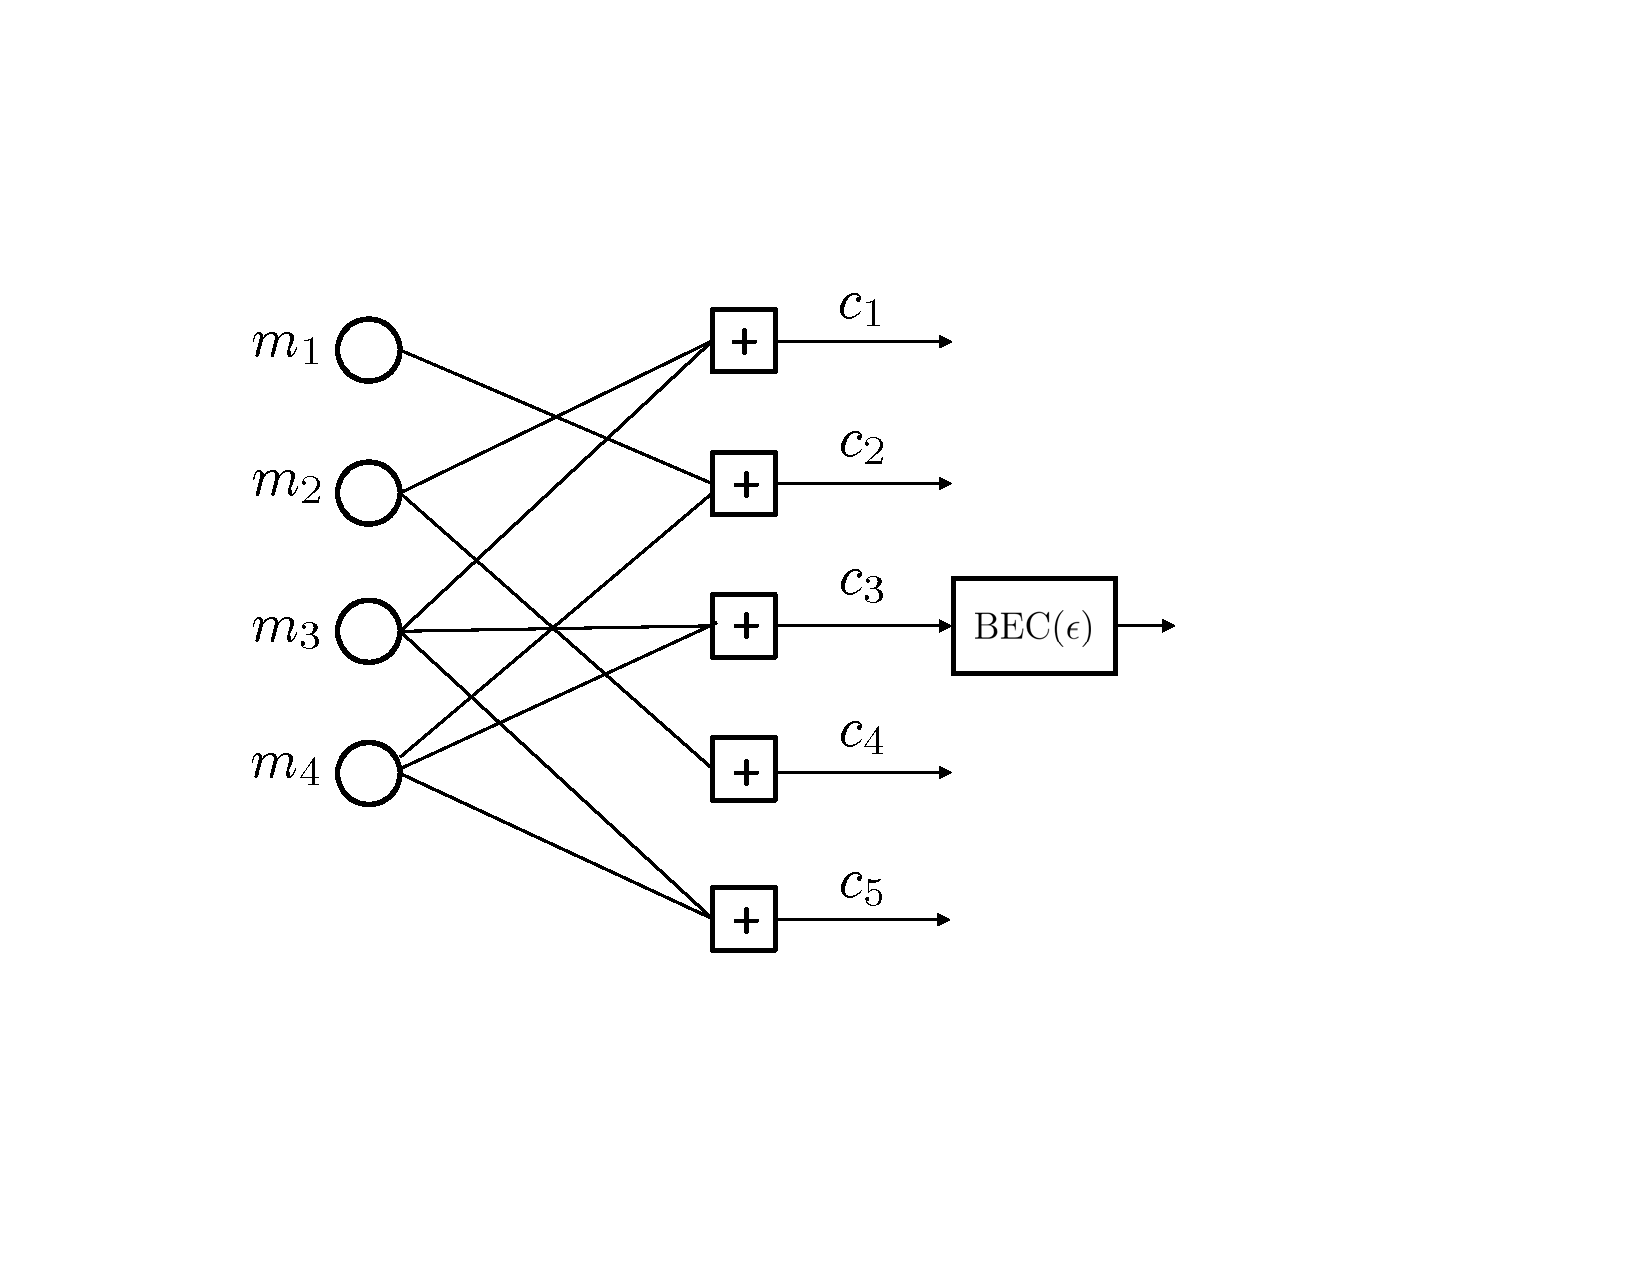
\includegraphics[width=2.0in]{LDGMoverbec}
%\end{center}
%\end{column}
%\begin{column}{0.47\textwidth}
%\begin{itemize}
%\item $L(x) = \frac14 x + \frac14 x^2 + \frac12 x^3$
%\vspace{2mm}
%\item $\lambda(x) = \frac19 + \frac29 x + \frac 69 x^2$
%\vspace{2mm}
%\item $R(x) = \frac15 x + \frac45 x^2$
%\vspace{2mm}
%\item $\rho(x) = \frac19 + \frac89 x$
%\vspace{2mm}
%\item Rate $R = \frac{\int_{0}^{1}\lambda(x) \ dx}{\int_{0}^{1} \rho(x) \ dx}$
%\end{itemize}
%\end{column}
%\end{columns}
%
%\begin{columns}
%\column{0.45\textwidth}
%\begin{block}{DE for LDPC}
%\vspace*{-3mm}
%\begin{eqnarray*}
%  x_0 &=& \epsilon \\
%  y_l &=& 1-\rho(1-x_{l-1}) \\
%  x_l &=& \epsilon \lambda(y_l)\\
%  x_l &=& \epsilon \lambda(1-\rho(1-x_{l-1}))
%\end{eqnarray*}
%\end{block}
%
%\column{0.45\textwidth}
%\begin{block}{DE for LDGM}
%\vspace*{-3mm}
%\begin{eqnarray*}
%  x_0 &=& 1 \\
%  y_l &=& 1-(1-\epsilon) \rho(1-x_{l-1}) \\
%  x_l &=& \lambda(y_l) \\
%  x_l &=& \lambda(1-(1-\epsilon)\rho(1-x_{l-1}))
%\end{eqnarray*}
%\end{block}
%\end{columns}
%\end{frame}
%%-------------------------------------------------------------------------------------
%\begin{frame}{What are rateless codes?}
%\begin{center}
%  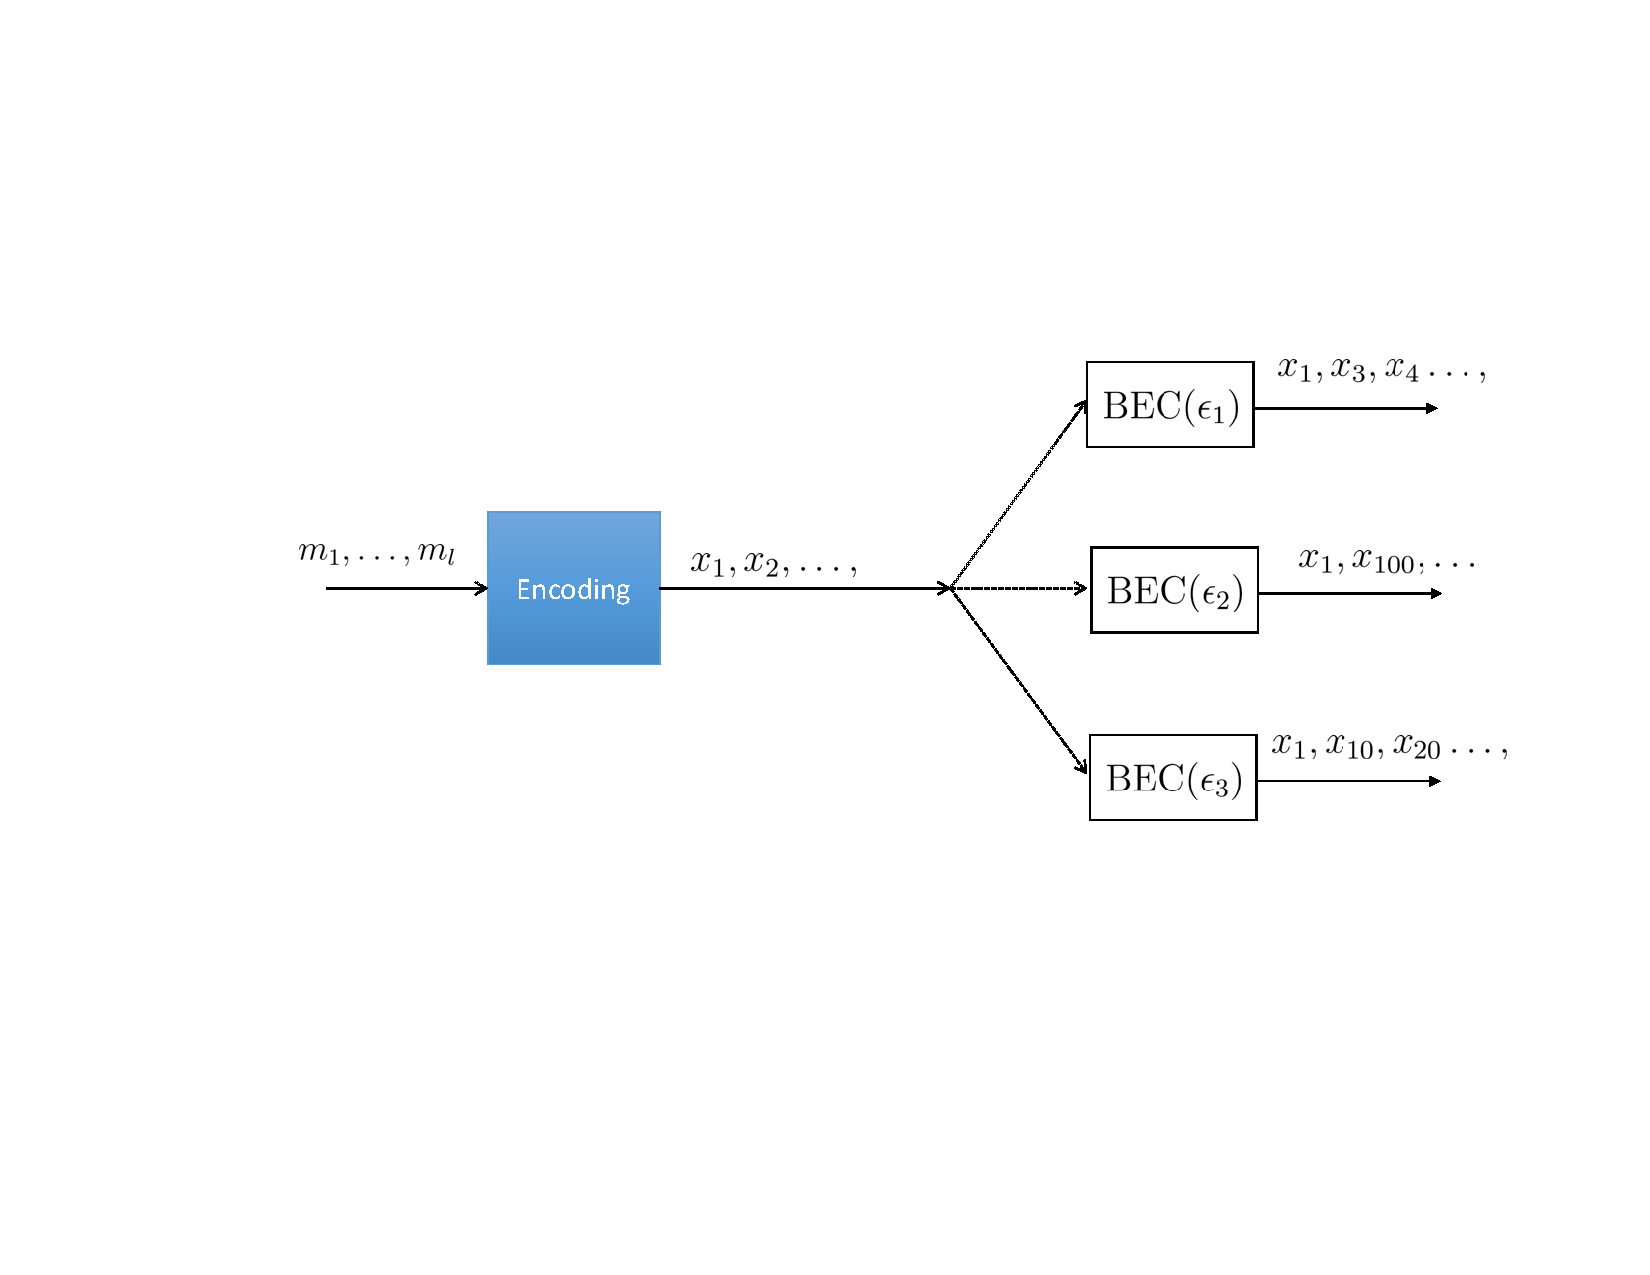
\includegraphics[width=3.5in]{ratelesssystem}
%\end{center}
%\begin{block}{Multicast with different channel qualities}
%\begin{itemize}
%\item Code should be simultaneously optimal for all $\epsilon$
%\item Want to create potentially endless stream of coded bits
%\end{itemize}
%\end{block}
%\pause
%\begin{block}{Downloading from multiple servers}
%\begin{itemize}
%\item Do not want to download the same coded bit multiple times
%\item Randomized encoding strategy is beneficial
%\end{itemize}
%\end{block}
%\end{frame}
%%--------------------------------------------------------------------------------------
%\begin{frame}{LDGM codes and rateless codes}
%\begin{center}
%  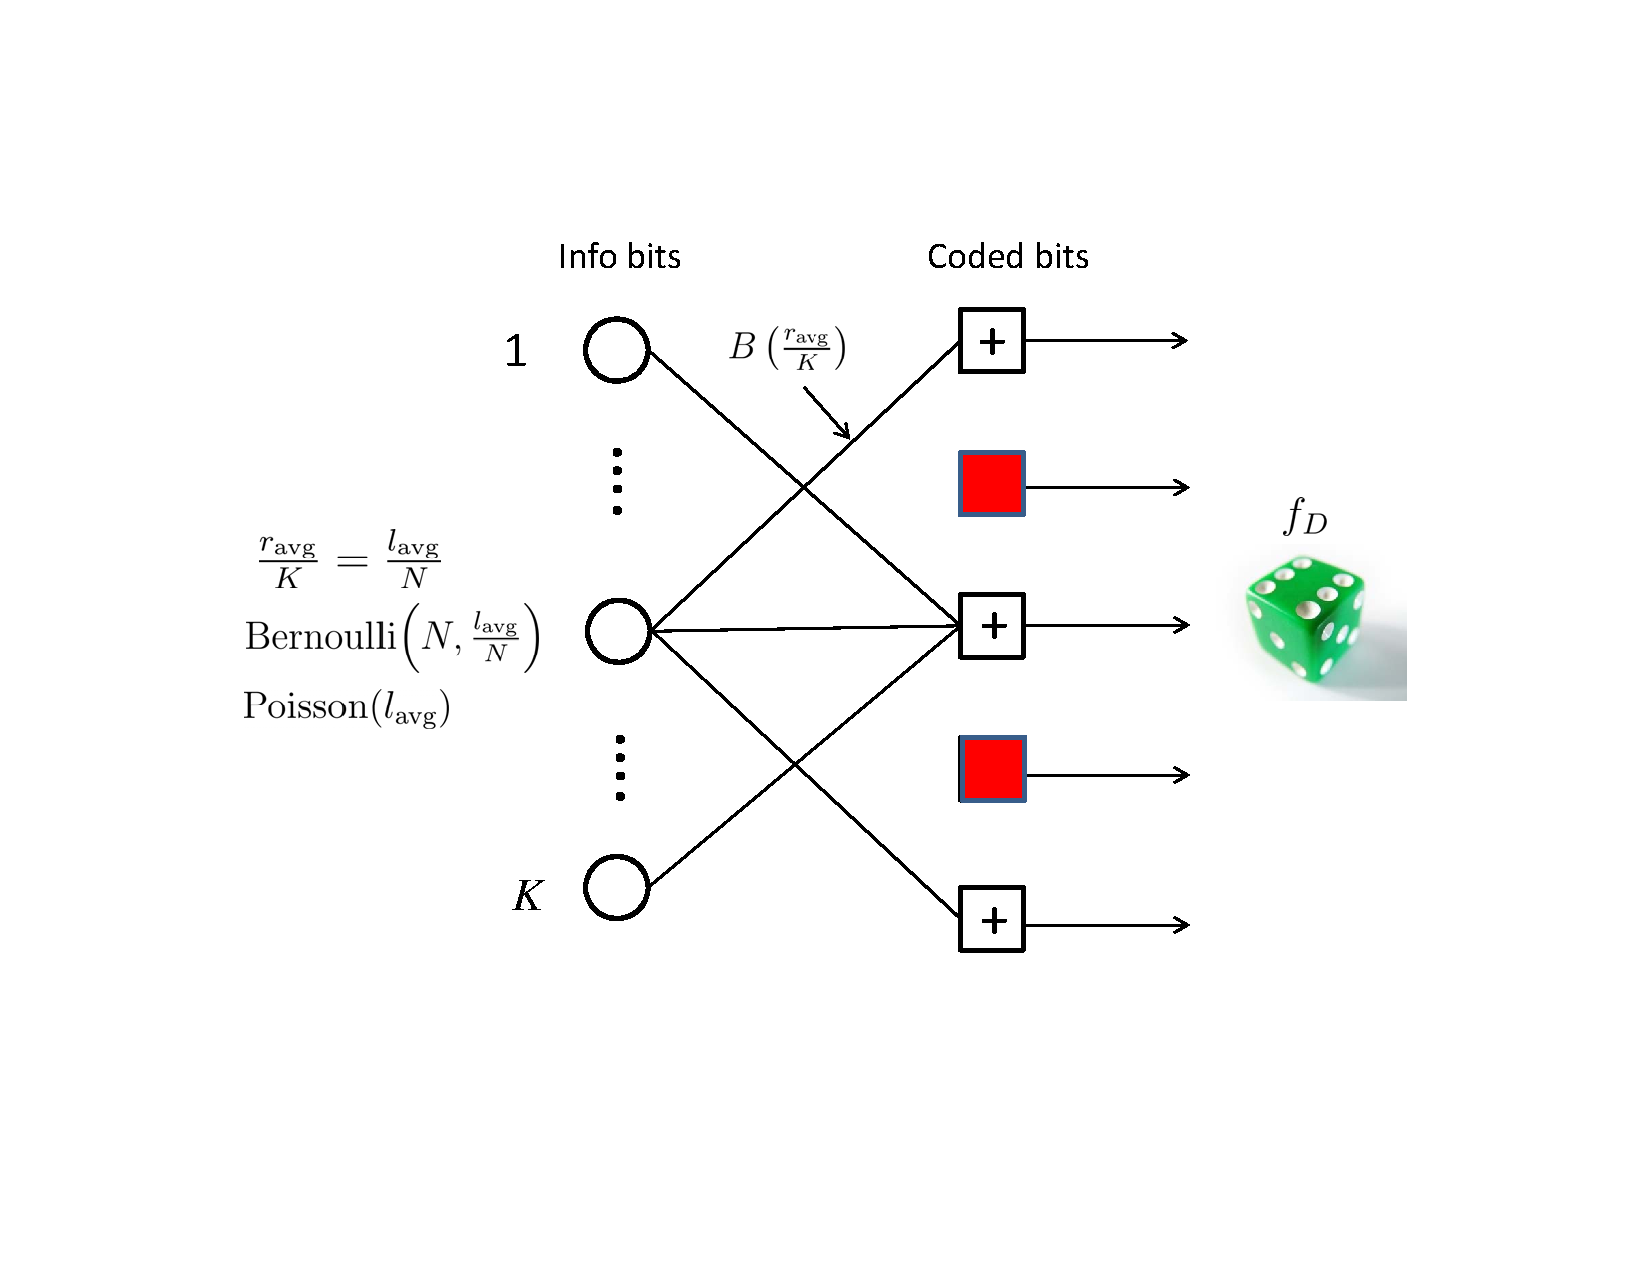
\includegraphics[width=2.75in]{ratelesserasures1}
%\end{center}
%
%\begin{block}{LT Codes, Luby'02}
%\begin{itemize}
%  \item Choose the degree according to a distribution $f_D$
%  \item Pick bits uniformly at random to make linear combination
%  \item Left degree is Poisson : $\lambda(x) = e^{-r_{avg}(1-x)}$
%\end{itemize}
%\end{block}
%\end{frame}
%%--------------------------------------------------------------------------------------
%\begin{frame}{Poisson, soliton pair is optimal for rateless codes}
%\vspace{-3mm}
%\begin{columns}
%\column{0.55\textwidth}
%\begin{center}
%\scalebox{0.45}{% This file was created by matlab2tikz v0.4.7 running on MATLAB 7.14.
% Copyright (c) 2008--2014, Nico Schlömer <nico.schloemer@gmail.com>
% All rights reserved.
% Minimal pgfplots version: 1.3
% 
% The latest updates can be retrieved from
%   http://www.mathworks.com/matlabcentral/fileexchange/22022-matlab2tikz
% where you can also make suggestions and rate matlab2tikz.
% 
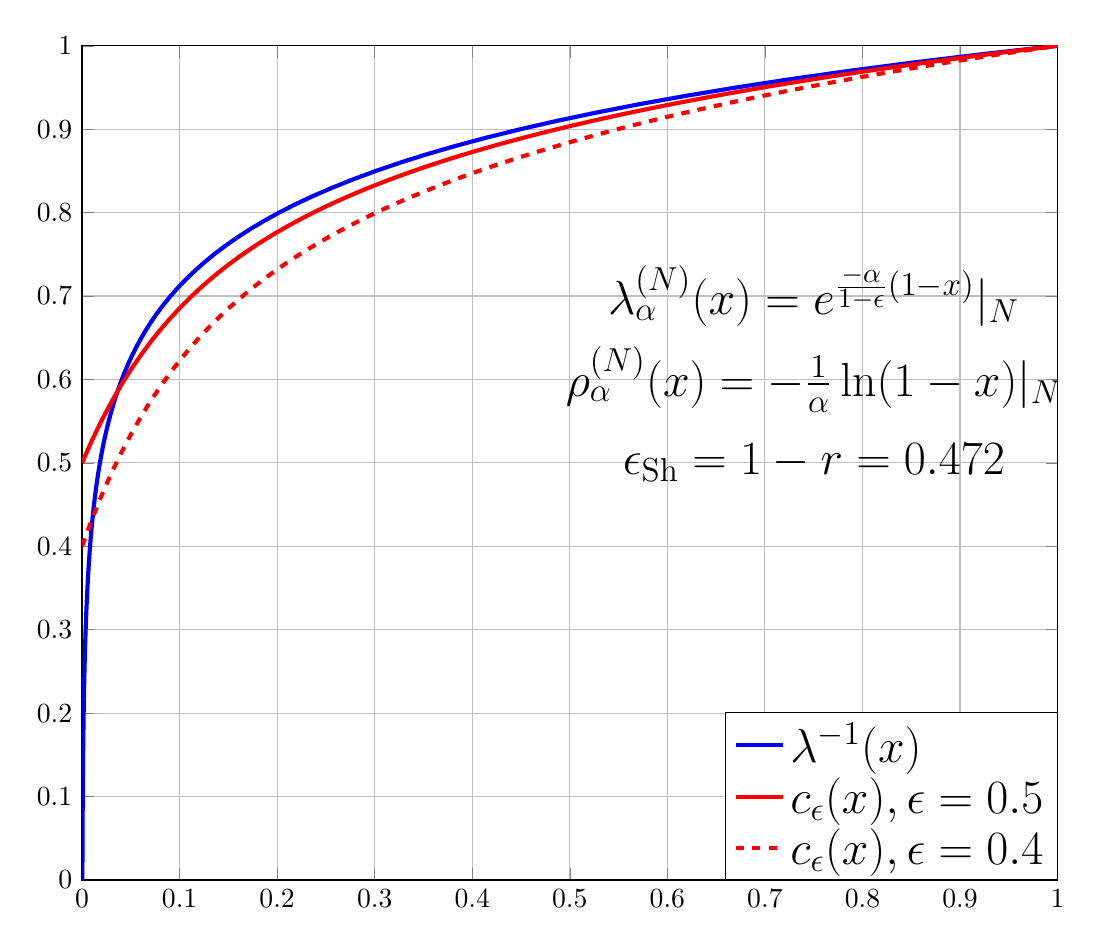
\begin{tikzpicture}
\def\fsize{\LARGE}

\begin{axis}[%
width=4.87804024496938in,
height=4.17068372703412in,
scale only axis,
xmin=0,
xmax=1,
xmajorgrids,
xtick={0,0.1,0.2,...,1},
xticklabels={0,0.1,0.2,0.3,0.4,0.5,0.6,0.7,0.8,0.9,1},
ymin=0,
ymax=1,
legend style={at={(1,0)},anchor=south east,draw=black,fill=white,legend cell align=left,font=\LARGE},
ymajorgrids
]
\node at (axis cs:0.75,0.7){\fsize{$\lambda_{\alpha}^{(N)}(x)=e^{\frac{-\alpha}{1-\epsilon} (1-x)}|_{N}$}};
%\sum\limits_{i=1}^{N}\frac{1}{\alpha}\frac{x^i}{i}}};
\node at (axis cs:0.75,0.6){\fsize{$\rho_{\alpha}^{(N)}(x)=-\frac{1}{\alpha}\ln (1-x)|_{N}$}};
%x^{\frac{1}{\alpha}},\alpha=0.1,N=50$}};
\node at (axis cs:0.75,0.5){\fsize{$\epsilon_{\text{Sh}}=1-r=0.472$}};

\addlegendentry{$\lambda^{-1}(x)$};
\addplot [color=blue,solid,line width=1.5pt]
  table[row sep=crcr]{0.000335494153584825	0\\
0.000363436477858997	0.01\\
0.000393706036385988	0.02\\
0.000426496657682508	0.03\\
0.000462018313674054	0.04\\
0.000500498464232096	0.05\\
0.000542183513693807	0.06\\
0.00058734038869107	0.07\\
0.000636258247392219	0.08\\
0.000689250331101526	0.09\\
0.000746655970072966	0.1\\
0.000808842756382345	0.11\\
0.000876208897771561	0.12\\
0.000949185767537662	0.13\\
0.00102824066679468	0.14\\
0.00111387981679615	0.15\\
0.00120665160047942	0.16\\
0.00130715007398865	0.17\\
0.00141601877066227	0.18\\
0.00153395482184343	0.19\\
0.00166171342090063	0.2\\
0.00180011265904357	0.21\\
0.00195003876389988	0.22\\
0.0021124517743976	0.23\\
0.00228839168829194	0.24\\
0.00247898512170151	0.25\\
0.00268545252329786	0.26\\
0.00290911598934362	0.27\\
0.00315140772962231	0.28\\
0.00341387923847058	0.29\\
0.00369821122963888	0.3\\
0.00400622439859745	0.31\\
0.00433989108120327	0.32\\
0.00470134788338308	0.33\\
0.00509290936270569	0.34\\
0.00551708284945217	0.35\\
0.00597658450208934	0.36\\
0.00647435669995645	0.37\\
0.00701358688453719	0.38\\
0.00759772796996556	0.39\\
0.00823052045346203	0.4\\
0.00891601636728181	0.41\\
0.00965860522554881	0.42\\
0.0104630421321226	0.43\\
0.0113344782294832	0.44\\
0.0122784936836085	0.45\\
0.0133011334160577	0.46\\
0.0144089458120634	0.47\\
0.0156090246524914	0.48\\
0.0169090545381691	0.49\\
0.0183173600974417	0.5\\
0.0198429592920402	0.51\\
0.0214956211625829	0.52\\
0.0232859283834527	0.53\\
0.0252253450275842	0.54\\
0.0273262899750436	0.55\\
0.0296022164354101	0.56\\
0.0320676980931018	0.57\\
0.0347385224271733	0.58\\
0.0376317918030286	0.59\\
0.0407660329832215	0.6\\
0.0441613157583836	0.61\\
0.0478393814576613	0.62\\
0.0518237821612379	0.63\\
0.0561400315059548	0.64\\
0.060815768049174	0.65\\
0.0658809322363014	0.66\\
0.0713679581043317	0.67\\
0.0773119809479292	0.68\\
0.0837510622765184	0.69\\
0.0907264335012647	0.7\\
0.098282759910384	0.71\\
0.106468426620664	0.72\\
0.115335848333247	0.73\\
0.124941804873458	0.74\\
0.135347804658769	0.75\\
0.146620478416798	0.76\\
0.15883200566779	0.77\\
0.172060576694392	0.78\\
0.186390892947055	0.79\\
0.201914709077521	0.8\\
0.218731420056951	0.81\\
0.23694869712112	0.82\\
0.256683176594334	0.83\\
0.278061205978336	0.84\\
0.301219652054399	0.85\\
0.326306776138336	0.86\\
0.353483182051611	0.87\\
0.382922842829663	0.88\\
0.41481421268376	0.89\\
0.449361431268097	0.9\\
0.486785627882633	0.91\\
0.527326333867846	0.92\\
0.571243012123746	0.93\\
0.618816713416241	0.94\\
0.670351869923472	0.95\\
0.726178237327734	0.96\\
0.786652997679963	0.97\\
0.852163036258837	0.98\\
0.923127406721123	0.99\\
1	1\\
};

\addlegendentry{$c_{\epsilon}(x),\epsilon=0.5$};
\addplot [color=red,solid,line width=1.5pt]
  table[row sep=crcr]{0	0.5\\
0.01	0.526526126042806\\
0.02	0.550706243040251\\
0.03	0.57280262188789\\
0.04	0.593046195873519\\
0.05	0.6116403489369\\
0.06	0.628764252863599\\
0.07	0.644575805441883\\
0.08	0.659214215869252\\
0.09	0.672802278552915\\
0.1	0.685448371847462\\
0.11	0.697248214159826\\
0.12	0.708286406177705\\
0.13	0.718637784699063\\
0.14	0.728368610616949\\
0.15	0.73753761100972\\
0.16	0.746196892968877\\
0.17	0.754392744735548\\
0.18	0.762166337885451\\
0.19	0.769554342676617\\
0.2	0.776589467232609\\
0.21	0.783300929956643\\
0.22	0.789714873441285\\
0.23	0.795854727138328\\
0.24	0.801741525169708\\
0.25	0.807394184880162\\
0.26	0.812829751044085\\
0.27	0.818063610032608\\
0.28	0.82310967771285\\
0.29	0.827980564381521\\
0.3	0.832687719622072\\
0.31	0.837241559611941\\
0.32	0.841651579088144\\
0.33	0.84592644990045\\
0.34	0.850074107836845\\
0.35	0.854101829192009\\
0.36	0.858016298362217\\
0.37	0.861823667586471\\
0.38	0.865529609810601\\
0.39	0.869139365526266\\
0.4	0.87265778432787\\
0.41	0.876089361835362\\
0.42	0.879438272548156\\
0.43	0.882708399123219\\
0.44	0.885903358507587\\
0.45	0.889026525300862\\
0.46	0.892081052675632\\
0.47	0.89506989114236\\
0.48	0.897995805409208\\
0.49	0.900861389555933\\
0.5	0.903669080713676\\
0.51	0.906421171418762\\
0.52	0.909119820787906\\
0.53	0.911767064644275\\
0.54	0.914364824708154\\
0.55	0.91691491695232\\
0.56	0.919419059210307\\
0.57	0.921878878115366\\
0.58	0.924295915438839\\
0.59	0.926671633888754\\
0.6	0.929007422422485\\
0.61	0.931304601121274\\
0.62	0.93356442566907\\
0.63	0.935788091473473\\
0.64	0.937976737462459\\
0.65	0.94013144958696\\
0.66	0.94225326405617\\
0.67	0.944343170329661\\
0.68	0.946402113887892\\
0.69	0.948430998800506\\
0.7	0.950430690109856\\
0.71	0.952402016045493\\
0.72	0.954345770083781\\
0.73	0.95626271286546\\
0.74	0.958153573982763\\
0.75	0.960019053646566\\
0.76	0.961859824243142\\
0.77	0.963676531789142\\
0.78	0.965469797292704\\
0.79	0.967240218027864\\
0.8	0.968988368728802\\
0.81	0.970714802709912\\
0.82	0.972420052917143\\
0.83	0.974104632915626\\
0.84	0.97576903781815\\
0.85	0.977413745158703\\
0.86	0.979039215714913\\
0.87	0.980645894282958\\
0.88	0.982234210408185\\
0.89	0.983804579074453\\
0.9	0.985357401354956\\
0.91	0.986893065027096\\
0.92	0.988411945153746\\
0.93	0.989914404633095\\
0.94	0.991400794719091\\
0.95	0.992871455514339\\
0.96	0.994326716437194\\
0.97	0.995766896664656\\
0.98	0.997192305552543\\
0.99	0.998603243034339\\
1	1\\
};

\addlegendentry{$c_{\epsilon}(x),\epsilon=0.4$};
\addplot [color=red,dashed,line width=1.5pt]
  table[row sep=crcr]{0	0.4\\
0.01	0.431831351251367\\
0.02	0.460847491648301\\
0.03	0.487363146265468\\
0.04	0.511655435048223\\
0.05	0.533968418724279\\
0.06	0.554517103436319\\
0.07	0.57349096653026\\
0.08	0.591057059043103\\
0.09	0.607362734263498\\
0.1	0.622538046216955\\
0.11	0.63669785699179\\
0.12	0.649943687413245\\
0.13	0.662365341638875\\
0.14	0.674042332740338\\
0.15	0.685045133211665\\
0.16	0.695436271562653\\
0.17	0.705271293682658\\
0.18	0.714599605462541\\
0.19	0.723465211211941\\
0.2	0.731907360679131\\
0.21	0.739961115947971\\
0.22	0.747657848129542\\
0.23	0.755025672565993\\
0.24	0.76208983020365\\
0.25	0.768873021856194\\
0.26	0.775395701252902\\
0.27	0.781676332039129\\
0.28	0.78773161325542\\
0.29	0.793576677257825\\
0.3	0.799225263546487\\
0.31	0.804689871534329\\
0.32	0.809981894905773\\
0.33	0.81511173988054\\
0.34	0.820088929404215\\
0.35	0.82492219503041\\
0.36	0.82961955803466\\
0.37	0.834188401103766\\
0.38	0.838635531772721\\
0.39	0.84296723863152\\
0.4	0.847189341193444\\
0.41	0.851307234202435\\
0.42	0.855325927057787\\
0.43	0.859250078947862\\
0.44	0.863084030209105\\
0.45	0.866831830361034\\
0.46	0.870497263210758\\
0.47	0.874083869370832\\
0.48	0.87759496649105\\
0.49	0.881033667467119\\
0.5	0.884402896856411\\
0.51	0.887705405702515\\
0.52	0.890943784945487\\
0.53	0.89412047757313\\
0.54	0.897237789649784\\
0.55	0.900297900342784\\
0.56	0.903302871052369\\
0.57	0.906254653738439\\
0.58	0.909155098526607\\
0.59	0.912005960666505\\
0.6	0.914808906906982\\
0.61	0.917565521345529\\
0.62	0.920277310802884\\
0.63	0.922945709768168\\
0.64	0.925572084954951\\
0.65	0.928157739504352\\
0.66	0.930703916867404\\
0.67	0.933211804395593\\
0.68	0.935682536665471\\
0.69	0.938117198560607\\
0.7	0.940516828131827\\
0.71	0.942882419254591\\
0.72	0.945214924100537\\
0.73	0.947515255438552\\
0.74	0.949784288779315\\
0.75	0.952022864375879\\
0.76	0.954231789091771\\
0.77	0.95641183814697\\
0.78	0.958563756751245\\
0.79	0.960688261633437\\
0.8	0.962786042474563\\
0.81	0.964857763251894\\
0.82	0.966904063500572\\
0.83	0.968925559498751\\
0.84	0.970922845381781\\
0.85	0.972896494190444\\
0.86	0.974847058857895\\
0.87	0.976775073139549\\
0.88	0.978681052489822\\
0.89	0.980565494889343\\
0.9	0.982428881625947\\
0.91	0.984271678032515\\
0.92	0.986094334184495\\
0.93	0.987897285559714\\
0.94	0.98968095366291\\
0.95	0.991445746617207\\
0.96	0.993192059724633\\
0.97	0.994920275997587\\
0.98	0.996630766663051\\
0.99	0.998323891641207\\
1	1\\
};
\end{axis}
\end{tikzpicture}}
%  %\includegraphics[width=2.2in]{EXIT_PoissSoliton}
%\end{center}
%\column{0.45\textwidth}
%\begin{center}
%  \includegraphics[width=2.2in]{ratelesserasures3}
%\end{center}
%\end{columns}
%%\begin{block}{Poisson, Soliton pair is optimal - $\lambda(x) = e^{-r_{avg}(1-x)}$}
%\begin{itemize}
%%\item Poisson, soliton pair is optimal
%  %\item Left degree is Poisson : $\lambda(x) = e^{-r_{avg}(1-x)}$
%  \item   $x = \lambda(1-(1-\epsilon)\rho(1-x))$
%  \item $\lambda(x) = e^{-\frac{\alpha}{1-\epsilon}(1-x)}$, \alert{optimal right degree is soliton: $\rho(x) = -\frac{1}{\alpha}\ln(1-x)$}
%  %\item \alert{Optimal distribution is soliton: $f_D[i] = \frac{1}{i(i-1)}$}
%\end{itemize}
%\begin{center}
%\begin{tabular}{|l|c|c|c|c|c|c|c|c|}
%\hline
%Degree of nodes & 1 & 2 & 3 & 4 & $\ldots$ & $i$ & \ldots & $K$ \\
%\hline
%Fraction: \alert{ $f_D[i]$ } & $\frac{1}{K}$ & $\frac12$ & $\frac16$ & $\frac{1}{12}$ & $\ldots$ & $\frac{1}{i(i-1)}$ & \ldots & $\frac{1}{K (K-1)}$ \\
%\hline
%\end{tabular}
%\end{center}
%%\end{block}
%\end{frame}
%%--------------------------------------------------------------------------------------
%\begin{frame}{Histogram of required $N$ for $K=10000$}
%\begin{center}
%  \includegraphics[width=4.2in]{fountaincodes10000histogram}
%\end{center}
%\begin{block}{Finite length considerations}
%\begin{itemize}
%  \item Deg. dist. must be adjusted for optimizing finite length performance
%  \item Raptor codes (Shokrollahi'06) is an excellent choice
%\end{itemize}
%\end{block}
%\end{frame}

%---------------------------------------------------------------------------------------
%\begin{frame}\frametitle{Questions?}
%	\begin{figure}[t]
%		\centering
%		
\includegraphics[width=2.8in]{questions}
%	\end{figure}
%	\centering
%	\color{blue}
%	%\Huge{Thank you!}
%\end{frame}
%---------------------------------------------------------------------------------------
\begin{frame}{Summary}
\begin{itemize}
  \item Understand what degree distributions $(\lambda(x),\rho(x))$ mean
\pause
  \item Given a $(\lambda,\rho)$ and $\epsilon$, what will be the $P_e^n$ as $l,n \rightarrow \infty$ ?
\pause
  \item Can you compute the threshold?
\pause
  \item Is a $(\lambda(x),\rho(x))$ pair optimal?
\end{itemize}
\end{frame} 

%\begin{frame}{Application 1}
\end{frame}
%--------------------------------------------------------------------------------------
\begin{frame}{The changing mobile landscape}
\begin{block}{}
\begin{itemize}
\item 5G will not only be ``4G but faster" but will support new models such as IoT
\item Current wireless - a few devices with sustained connectivity
\item Future wireless -  \alert{massive} no. of devices requesting \alert{sporadic} connectivity
\end{itemize}
\end{block}
\begin{center}
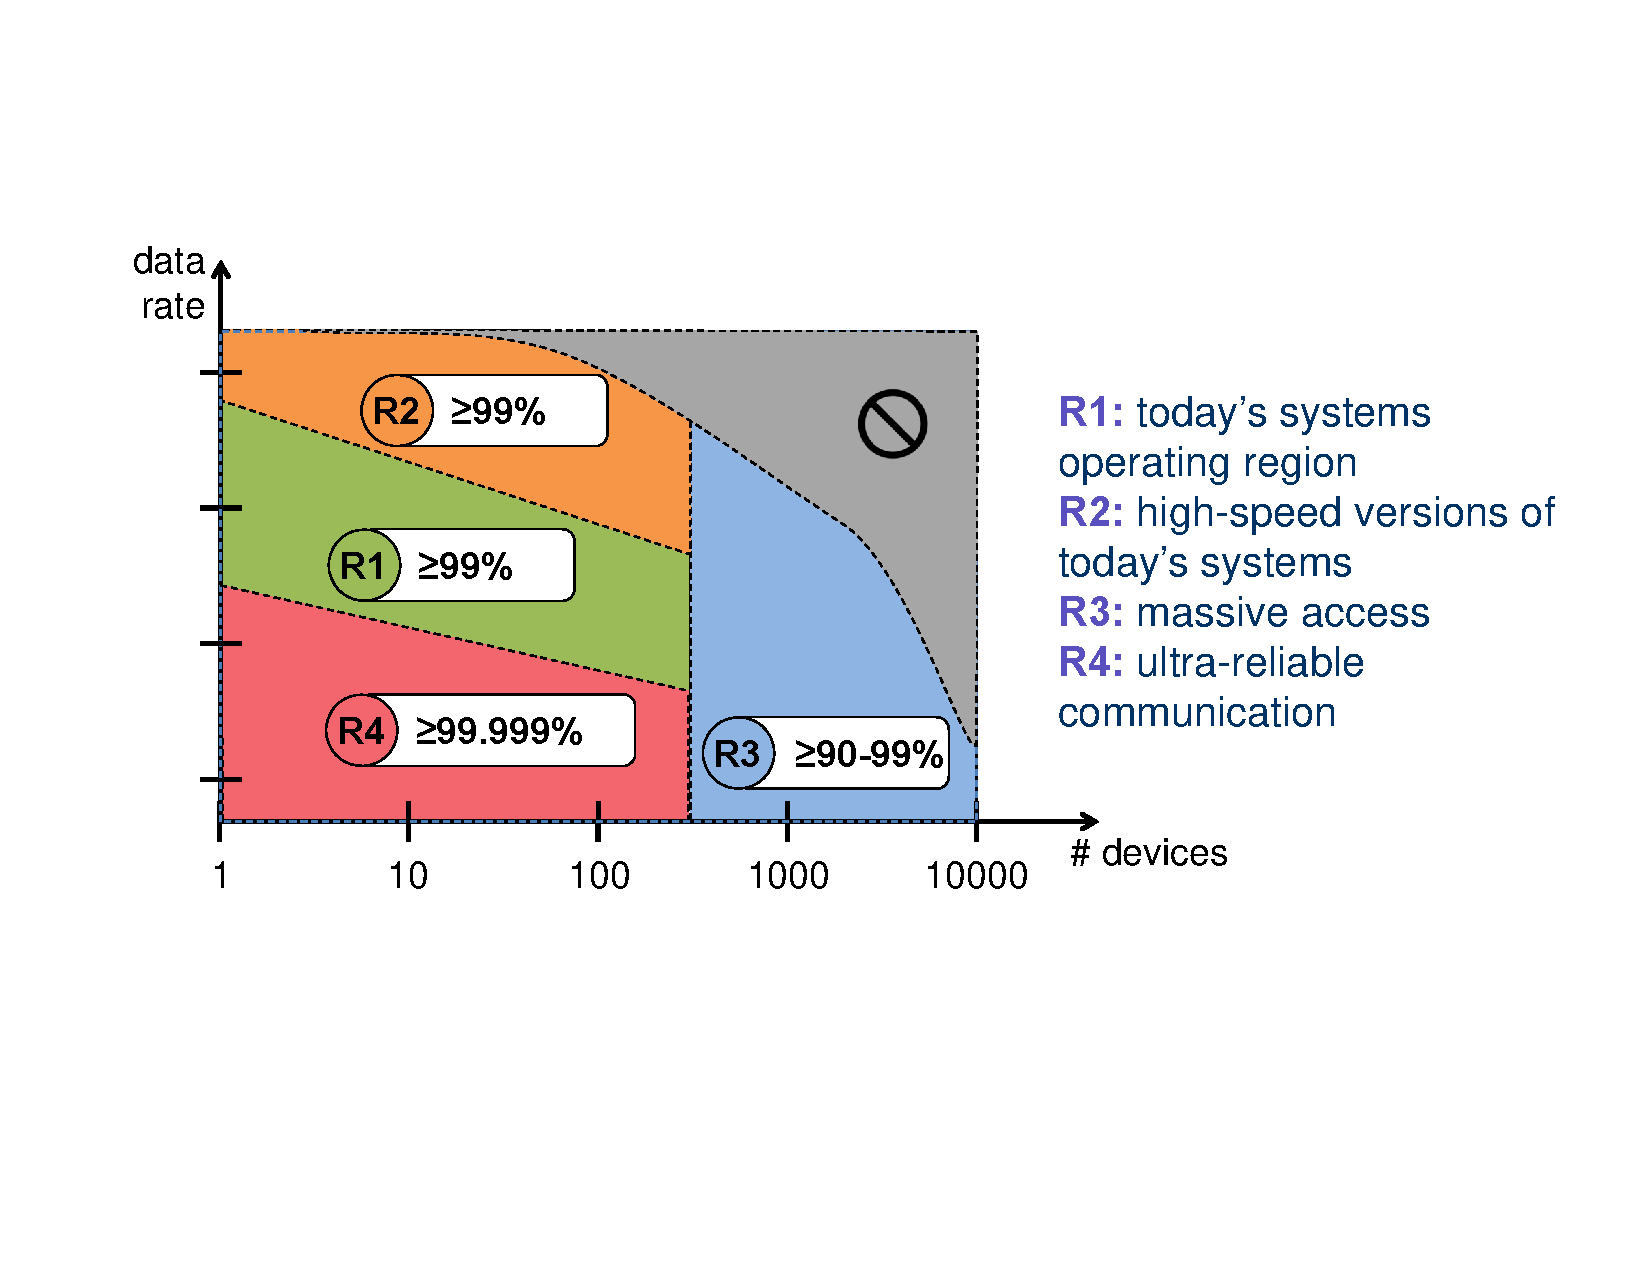
\includegraphics[width=4.5in]{C:/Users/nrkri/Dropbox/Work/RESEARCH/Projects/MACcollision/Figures/5Gchanginglandscape}
\end{center}
\end{frame}
%------------------------------------------------------------------------------------
\begin{frame}{The changing mobile landscape}
\begin{block}{}
\begin{itemize}
%\item 5G will not only be ``4G but faster" but will support new models such as IoT
\item Current wireless - a few devices with sustained connectivity
\item Future wireless -  \alert{many uncoordinated} devices requesting \alert{sporadic} connectivity
\end{itemize}
\end{block}
\begin{center}
\includegraphics[width=2.75in]{C:/Users/nrkri/Dropbox/Work/RESEARCH/Projects/MACcollision/Figures/machinetomachine}
\end{center}
\end{frame}
%------------------------------------------------------------------------------------
\begin{frame}{The changing mobile landscape}
\begin{block}{}
\begin{itemize}
%\item 5G will not only be ``4G but faster" but will support new models such as IoT
\item Current wireless - a few devices with sustained connectivity
\item Future wireless -  \alert{many uncoordinated} devices requesting \alert{sporadic} connectivity
\end{itemize}
\end{block}
\begin{center}
\includegraphics[width=2.75in]{C:/Users/nrkri/Dropbox/Work/RESEARCH/Projects/MACcollision/Figures/vehicular_sensor_networks}
\end{center}
\end{frame}
%------------------------------------------------------------------------------------
\begin{frame}{A possible MAC frame structure}
\begin{itemize}
\item Total of $Q$ users out of which $K$ are active
\item $Q$ is very large and $K$ is a small fraction of $Q$
\end{itemize}
\begin{figure}[t!]
  \begin{center}
  %\scalebox{0.85}{\input{../../Projects/MACcollision/Figures/slotstructurewithoutfb}}
\begin{center}
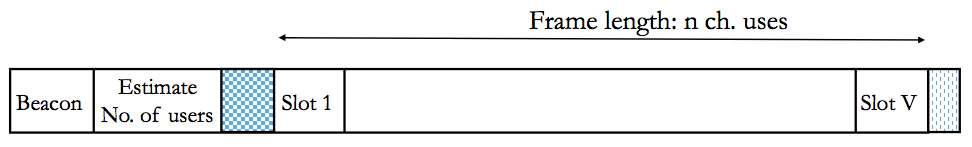
\includegraphics[width=4.5in]{C:/Users/nrkri/Dropbox/Work/RESEARCH/Projects/MACcollision/Figures/slotstructurewithoutfb}
\end{center}
%  \caption{At the onset of a frame, the base station heralds the start of a new round, and transmits a beacon for coarse synchronization. It then estimates the number of active devices, and subsequently broadcasts the number of slots contained within the frame. This header is followed by a sequence of time slots during which codewords are transmitted in a largely uncoordinated manner.}
%  \caption{Proposed structure: synchronization beacon, population estimation, slot sequence, \& feedback.}
%  \label{fig:framework}
  \end{center}
\end{figure}
\begin{itemize}
\item Beacon is used to obtain coarse synchronization
\item Each user transmits a signature sequence
\item BS estimates the no. of users ($K$) (Chen, Guo '14, Calderbank)
\item Picks an $M$ and broadcasts it
\end{itemize}
\end{frame}

%------------------------------------------------------------------------------------

\begin{frame}{System under consideration}
\begin{itemize}
\item Wireless network with \textcolor{blue}{$K$ distributed users} (no coordination)
\item Each user has one packet of info to transmit to a central receiver
\item Total \textcolor{red}{time is split into $M$ slots} (packet duration)
    \begin{itemize}
    \item Some policy used to decide if they transmit in $j$-th slot or not
    \item Receiver knows the set of users transmitting in the $j$-th slot
    \end{itemize}
\end{itemize}
\vspace*{-0.1in}
\begin{center}
\includegraphics[width=2.5in]{C:/Users/nrkri/Dropbox/Work/RESEARCH/Projects/MACcollision/Figures/systemmodel1}
\end{center}
\end{frame}

%------------------------------------------------------------------------------------
\begin{frame}{Random access paradigm}
\begin{itemize}
\item $k$-th user:
\begin{itemize}
  \item Generates a random variable $D_k \in \{1,\ldots,M\}$
  \item Generating PMF is $f_D$, i.e., \alert{$Pr(D_k=i) = f_D[i]$}
  \item Transmits during $D_k$ time slots drawn uniformly from $\{1,\ldots,M\}$
\end{itemize}
\end{itemize}
\begin{center}
\includegraphics[width=2.5in]{C:/Users/nrkri/Dropbox/Work/RESEARCH/Projects/MACcollision/Figures/systemmodel2}
\end{center}
\vspace{-3mm}
\begin{itemize}
\item In this example, $D_3 = 3$ and user 3 transmits in slots $\{1,3,5\}$
%\item Our setup is based on Liva 2011 \& Paolini et al. 2012
\end{itemize}
\end{frame}
%------------------------------------------------------------------------------------
\begin{frame}{Iterative interference cancelation}
\begin{itemize}
\item \textcolor{red}{If exactly one user transmits per slot, then packet is decoded w.h.p.}
\vspace{1mm}
\item \textcolor{blue}{If more than one user transmits per slot, then collision}
    \begin{itemize}
\vspace{1mm}
    \item Rx subtracts previously decoded packets from collided packets
\vspace{1mm}
    \item If Rx can subtract all but one, remaining packet is decoded w.h.p.
\vspace{1mm}
    \item Otherwise, the received packet is saved for future processing
\vspace{1mm}
    \item Once all $K$ packets recovered, an ACK terminates the transmission
\vspace{1mm}
    \item Similar to interference cancellation in multi-user detection
    \end{itemize}
\end{itemize}
\vspace*{-0.1in}
\begin{center}
\includegraphics[width=2.5in]{C:/Users/nrkri/Dropbox/Work/RESEARCH/Projects/MACcollision/Figures/iterativeinterferencecancellation2}
\end{center}
\end{frame}
%------------------------------------------------------------------------------------
\begin{frame}{Performance measure - Efficiency}
 \begin{itemize}
    \item Suppose \textcolor{red}{$M$ time slots} needed to successfully transmit all $K$ packets
\vspace{6mm}
    \item Then, the \textcolor{blue}{efficiency of the system} is said to be \[\eta = K/M \; \text{packets/slot} \]
 \end{itemize}
\end{frame}
%------------------------------------------------------------------------------------
\begin{frame}{Graphical representation (Liva 2012)}
\begin{itemize}
\item Tanner graph representation for the transmission scheme
\item Variable nodes $\leftrightarrow$ users, Check nodes $\leftrightarrow$ received packets
\item Message-passing decoder - \textcolor{blue}{peeling decoder} for the erasure channel
\end{itemize}
\begin{center}
\includegraphics[width=3.75in]{./Figures/iterativeinterferencecancellation2}
\end{center}
%\begin{minipage}[t]{0.48\linewidth}
%\begin{center}
%\includegraphics[width=1.75in]{../../Projects/MACcollision/Figures/graphicalmodel}
%\end{center}
%\end{minipage}
%\begin{minipage}[t]{0.48\linewidth}
%\begin{center}
%\includegraphics[width=1.75in]{../../Projects/MACcollision/Figures/graphicalmodelmsgpassing}
%\end{center}
%\end{minipage}
\pause
\begin{block}{}
\begin{itemize}
\item $L_i$ ($R_i$) - fraction of left (right) nodes with degree $i$ - notice that $\boxed{L_i = f_D[i]}$
\item $\lambda_i$ ($\rho_i$) - fraction of edges connected to left (right) nodes with deg $i$
\end{itemize}
\end{block}
\end{frame}
%%------------------------------------------------------------------------------------
\begin{frame}{Low density generator matrix (LDGM) codes}
\vspace{-3mm}
\begin{columns}
\begin{column}{0.47\textwidth}
\begin{center}
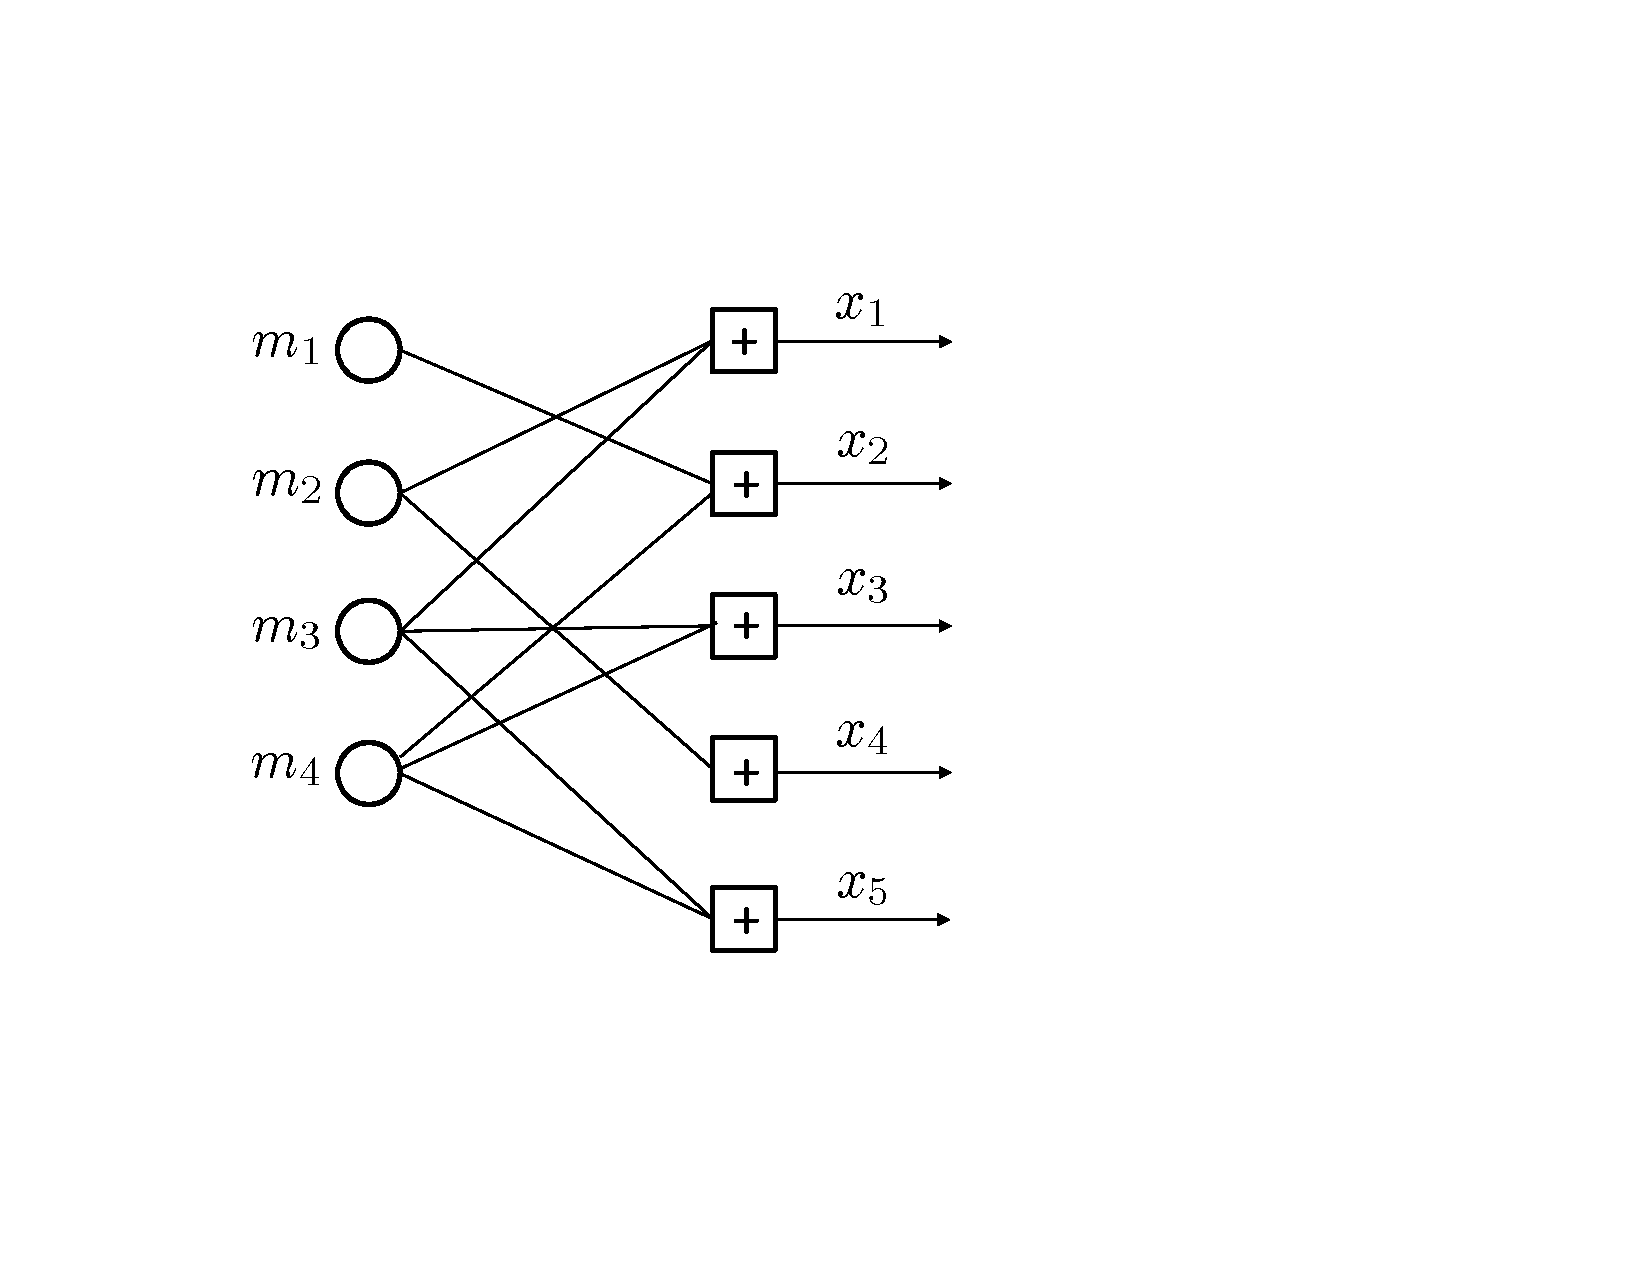
\includegraphics[width=2.0in]{./Figures/LDGM}
\end{center}
\end{column}
\begin{column}{0.47\textwidth}
\begin{itemize}
\item $L(x) = \frac14 x + \frac14 x^2 + \frac12 x^3$
\vspace{2mm}
\item $\lambda(x) = \frac19 + \frac29 x + \frac 69 x^2$
\vspace{2mm}
\item $R(x) = \frac15 x + \frac45 x^2$
\vspace{2mm}
\item $\rho(x) = \frac19 + \frac89 x$
\vspace{2mm}
\item Rate $R = \frac{\int_{0}^{1}\lambda(x) \ dx}{\int_{0}^{1} \rho(x) \ dx}$
\end{itemize}
\end{column}
\end{columns}

\begin{columns}
\column{0.45\textwidth}
\begin{block}{DE for LDPC}
\vspace*{-3mm}
\begin{eqnarray*}
  x_0 &=& \epsilon \\
  y_l &=& 1-\rho(1-x_{l-1}) \\
  x_l &=& \epsilon \lambda(y_l)\\
  x_l &=& \epsilon \lambda(1-\rho(1-x_{l-1}))
\end{eqnarray*}
\end{block}

\column{0.45\textwidth}
\begin{block}{DE for LDGM}
\vspace*{-3mm}
\begin{eqnarray*}
  x_0 &=& 1 \\
  y_l &=& 1-\rho(1-x_{l-1}) \\
  x_l &=& \lambda(y_l) \\
  x_l &=& \lambda(1-\rho(1-x_{l-1}))
\end{eqnarray*}
\end{block}
\end{columns}
\end{frame}
%%------------------------------------------------------------------------------------
%\begin{frame}{Analysis of the scheme - degree distributions}
%%\begin{block}{}
%%\begin{itemize}
%%\item $L_i$ ($R_i$) - no. of left (right) nodes with degree $i$
%%\item $\lambda_i$ ($\rho_i$) - no. of edges connected to left (right) nodes with deg $i$
%%\end{itemize}
%%\end{block}
%\begin{itemize}
%\item For a given $f_D$, the scheme results in an ensemble of LDGM codes
%\vspace{2mm}
%\begin{itemize}
%\item VN d.d. from node perspective - $L(x) = \sum_i L_i x^i$ ($L_i = f_D[i]$)
%\vspace{1mm}
%\item VN d.d. from edge perspective - $\lambda(x) = \sum_i \lambda_i x^{i-1} = \frac{L'(x)}{L'(1)}$
%\vspace{1mm}
%\item CN d.d. from node perspective - $R(x) = \sum_i R_i x^i$
%\vspace{1mm}
%\item CN d.d. from edge perspective - $\rho(x) =\sum_i \rho_i x^{i-1} = \frac{R'(x)}{R'(1)}$
%\end{itemize}
%\item ${\texttt{l}}_{avg} = L'(1)$ and ${\texttt{r}}_{avg} = \frac{K}{M} {\texttt{l}}_{avg}$
%\end{itemize}
%
%\begin{block}{Efficiency of the scheme}
%\[
%\eta = \frac{K}{M} = \frac{{\texttt r}_{avg}}{{\texttt l}_{avg}} =
%\frac{R'(1)}{L'(1)}
%\]
%\end{block}
%\end{frame}
%%------------------------------------------------------------------------------------
%\begin{frame}{Example of degree distributions}
%\begin{columns}
%\begin{column}{0.47\textwidth}
%\begin{center}
%\includegraphics[width=1.75in]{../Figures/graphicalmodel}
%\end{center}
%\end{column}
%\begin{column}{0.47\textwidth}
%\begin{itemize}
%\item $L(x) = \frac14 x + \frac14 x^2 + \frac12 x^3$
%\vspace{3mm}
%\item $\lambda(x) = \frac19 + \frac29 x + \frac 69 x^2$
%\vspace{3mm}
%\item $R(x) = \frac15 x + \frac45 x^2$
%\vspace{3mm}
%\item $\rho(x) = \frac19 + \frac89 x$
%\end{itemize}
%\end{column}
%\end{columns}
%\end{frame}
%------------------------------------------------------------------------------------
\begin{frame}{Poisson approximation for check node d.d.}

\vspace{-0.15in}
\begin{center}
\hspace{14mm} \includegraphics[width=2.0in]{C:/Users/nrkri/Dropbox/Work/RESEARCH/Projects/MACcollision/Figures/poissonapprox}
\end{center}
\vspace{-0.15in}
\begin{block}{Slot transmission probability}
User $k$ transmits in slot $m$ with prob. $p = \sum_{i=1}^\infty L_i \frac{i}{M} = \frac{\texttt{l}_{avg}}{M} = \frac{\texttt{r}_{avg}}{K}$ \pause
\end{block}
\begin{block}{Optimal multiple access policy}
%\vspace*{-0.1in}
%\begin{eqnarray}
%\nonumber
%R_i & = & \frac{\texttt{r}_{avg}^i e^{-\texttt{r}_{avg}}}{i!} \Rightarrow R(x) = \sum_i \frac{\texttt{r}_{avg}^i e^{-\texttt{r}_{avg}}}{i!} x^i \\
%\nonumber
%& \Rightarrow & \ R(x) \rightarrow e^{-{\texttt{r}}_{avg}(1-x)}, \ \ \ \rho(x) \rightarrow e^{-{\texttt{r}}_{avg}(1-x)}
%\end{eqnarray}
\begin{itemize}
\item Poisson approximation for $R(x)$ as $K,M \rightarrow \infty$
\item Finding optimal $f_D$ - same as finding optimal $\lambda(x)$ for $\rho(x) = e^{-{\texttt{r}}_{avg}(1-x)}$
\end{itemize}
\end{block}
\end{frame}
%------------------------------------------------------------------------------------
\begin{frame}{Intuition behind the main result (Narayanan,Pfister'12)}
%\small
\begin{block}{Convergence condition : $\rho(1-\lambda(y)) > 1-y$}
\begin{align*}
\rho(1-\lambda(y)) &= 1-y \\
e^{-\texttt{r}_{avg} \lambda(y)} &= e^{\ln(1-y)}\\
\Rightarrow -\texttt{r}_{avg} \lambda(y)&= \ln(1-y) = -\sum_{i=1}^{\infty} \frac{y^i}{i}\\
\Rightarrow \texttt{r}_{avg} \sum_i \lambda_i y^i & = \sum_{i=1}^{\infty} \frac{y^i}{i}
\end{align*}
\end{block}
%\begin{itemize}
%\item Analyze numerator of $\lambda^N(x)$ using $-\ln(1-x) = \sum_{i=1}^{\infty} \frac{x^i}{i}$
%\item For $y\in(0,1)$, $-ay + \sum_{i=1}^{N} \frac{y^i}{i} < -ay -\ln(1-y)$
%\item $\rho^N(1-\lambda^N(y)) = e^{ay-\sum_{i=1}^N \frac{y^i}{i}} > e^{\ln(1-y)} e^{ay} > (1-y)$
%\end{itemize}
%\end{block}
%\vspace{-1mm}
\pause
\begin{block}{}
\begin{align*}
\texttt{r}_{avg} \lambda_i &= \frac{1}{i}\\
\sum_i \lambda_i & = 1 \Rightarrow \boxed{\texttt{r}_{avg} = \sum_i \frac{1}{i}, \lambda_i = \frac{1/i}{\sum_i 1/i}} \Rightarrow \boxed{L_i = \frac{1}{i(i-1)}, i\geq2}
\end{align*}
\end{block}
\end{frame}
%%------------------------------------------------------------------------------------
%\begin{frame}{Finding optimal $f_D$}
%\begin{block}{Finding optimal $f_D$ - same as finding optimal $\lambda(x)$ for $\rho(x) = e^{-{\texttt{r}}_{avg}(1-x)}$}
%\end{block}
%%\pause
%%\begin{block}{Optimal distribution is soliton: $f(i) = \frac{1}{i(i-1)}$}
%%\begin{center}
%%\begin{tabular}{|l|c|c|c|c|c|c|}
%%\hline
%%No. of times & 1 & 2 & 3 & 4 & $\ldots$ & $M$ \\
%%\hline
%%Fraction of users & 0 & $\frac12$ & $\frac16$ & $\frac{1}{12}$ & $\ldots$ & $\frac{1}{M (M-1)}$ \\
%%\hline
%%\end{tabular}
%%\end{center}
%%\end{block}
%%\pause
%% \begin{block}{}
%% {For any $a\in[0,1]$, consider the sequence (indexed by $N\in \mathbb{N}$) of node-perspective degree-distributions,  $(L^N(x),R^N(x))$, where
%%\begin{align*}
%%L^N(x) &= \frac{\sum_{i=2}^{N+1}\frac{x^i}{i(i-1)}-\frac{a x^2}{2}}{\sum_{i=2}^{N+1}\frac{1}{i(i-1)}-\frac{a}{2}} \\
%%R^N(x) &= e^{-\left(H(N)-a\right)(1-x)}.
%%\end{align*}
%%Here $H(N) = \sum_{i=1}^N \frac{1}{i}$ is the $N$-th Harmonic number. For every ensemble in this sequence, ${\sf y}_\ell \stackrel{\ell \rightarrow \infty}{\rightarrow} 0$ while $\eta^N = \frac{N}{N+1} - a \stackrel{N \rightarrow \infty}{\rightarrow} 1-a$.}
%%\end{block}
%%\pause
%%\begin{block}{Average degree and its consequences}
%%\begin{itemize}
%%\item Average left degree is $\ln M \Rightarrow $ average right degree is $\eta \ln M$
%%\item For $K,M \rightarrow \infty$, $\texttt{r}_{avg} \rightarrow \infty \Rightarrow P$(right degree $=1) \rightarrow 0$
%%\pause
%%\item Consequence 1: Iterations can get stuck at the beginning
%%\item Consequence 2: Average power consumed is $\ln K$ times larger
%%\end{itemize}
%%\end{block}
%\end{frame}

%%------------------------------------------------------------------------------------
%\begin{frame}{Connection with Luby Transform (LT) codes}
%\begin{itemize}
%\item Clearly, the coding paradigm is similar to that of rateless codes
%\item The main difference is that data is not centrally available
%\end{itemize}
%\begin{center}
%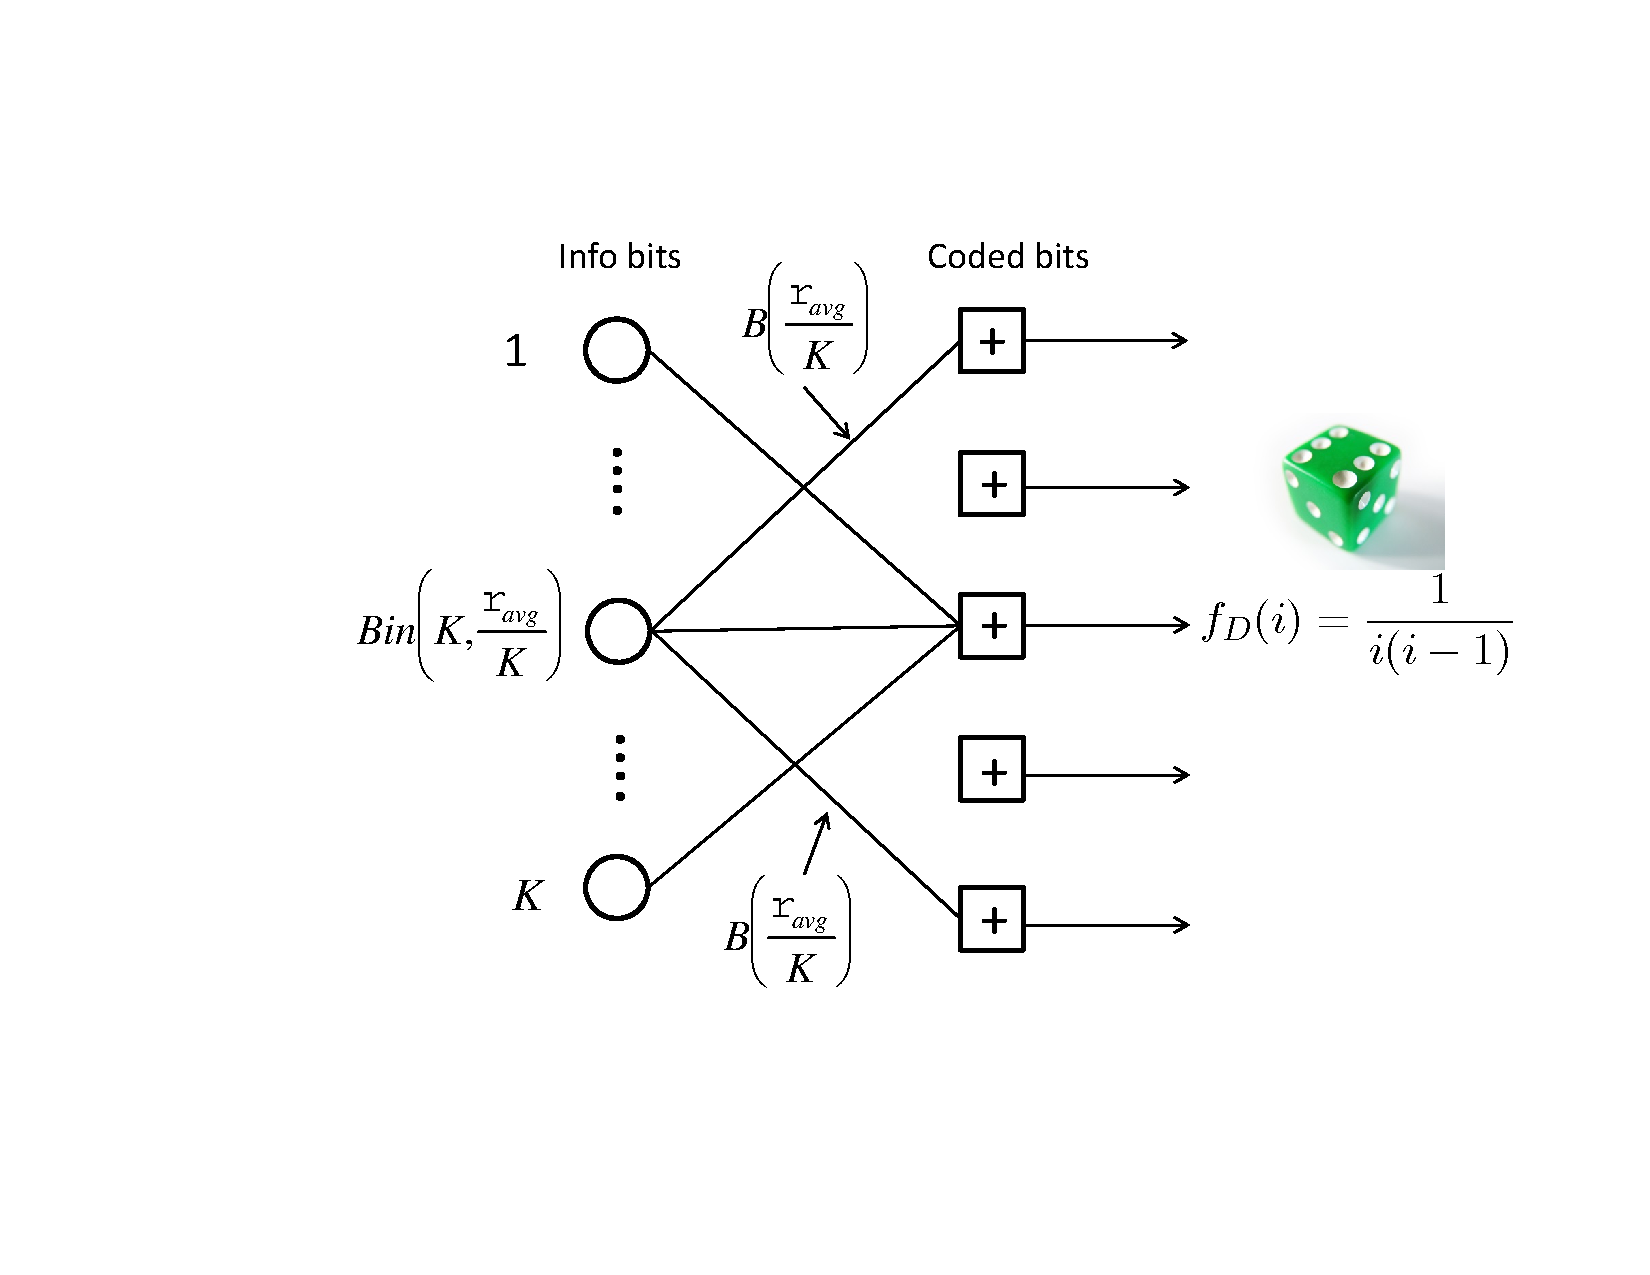
\includegraphics[width=2.5in]{../../Projects/MACcollision/Figures/rateless}
%\end{center}
%%\vspace{2mm}
%\begin{itemize}
%\item From a mathematical point of view
%    \begin{itemize}
%    \item Uncoordinated erasures imply LT codes must have a Poisson bit d.d. and optimality gives $\rho(x) \!= -\ln(1-x)$
%    \item Uncoordinated transmission implies coded ALOHA has a Poisson check d.d. and optimality gives $\lambda(x) \!= -\ln(1-x)$
%    \item \textcolor{red}{Both these pairs are optimal for the iterative process!}
%    \end{itemize}
%\end{itemize}
%%\pause
%\pause
%\begin{itemize}
%\item In some ways, Soliton d.d. is more natural here than for LT codes
%\item An outer code is not required to recover bits that are left uncovered by the encoding process
%\end{itemize}
%\end{frame}
%------------------------------------------------------------------------------------
\begin{frame}{Graphical interpretation - EXIT chart}
\begin{center}
\includegraphics[width=3.5in]{C:/Users/nrkri/Dropbox/Work/RESEARCH/Projects/MACcollision/Figures/DEsoliton}
\end{center}
\end{frame}
%-------------------------------------------------------------------------------
\begin{frame}{Main result}
\begin{block}{}
\begin{itemize}
\item For coordinated transmission, clearly $\eta = 1$,
\pause
\item ALOHA provides $\eta \approx 0.37$
\pause
\item But, even for uncoordinated transmission, $\eta \rightarrow 1$ as $K \rightarrow \infty$
\end{itemize}
\end{block}
\pause
\begin{block}{Optimal distribution is soliton: $f_D[i] = \frac{1}{i(i-1)}$}
\begin{center}
\begin{tabular}{|l|c|c|c|c|c|c|}
\hline
No. of times & 1 & 2 & 3 & 4 & $\ldots$ & $M$ \\
\hline
Fraction of users & $\frac{1}{M}$ & $\frac12$ & $\frac16$ & $\frac{1}{12}$ & $\ldots$ & $\frac{1}{M (M-1)}$ \\
\hline
\end{tabular}
\end{center}
\end{block}
\end{frame}
%--------------------------------------------------------------------------------------
\begin{frame}{Balls in bins}
\begin{itemize}
  \item $M$ balls thrown into $N$ bins uniformly at random
  \item If every bin has to be non-empty with prob $1-\delta$, how large should $M$ be ? \pause $\boxed{N \log \frac{N}{\delta}}$
  \item For the multiple access problem, an empty bin means a wasted time slot
  \item Note that for the soliton the average number of edges is indeed $N \log N)$
\end{itemize}
\end{frame}
%--------------------------------------------------------------------------------------
\begin{frame}{Poisson, soliton pair is optimal for rateless codes}
\vspace{-3mm}
\begin{columns}
\column{0.55\textwidth}
\begin{center}
\scalebox{0.45}{% This file was created by matlab2tikz v0.4.7 running on MATLAB 7.14.
% Copyright (c) 2008--2014, Nico Schlömer <nico.schloemer@gmail.com>
% All rights reserved.
% Minimal pgfplots version: 1.3
% 
% The latest updates can be retrieved from
%   http://www.mathworks.com/matlabcentral/fileexchange/22022-matlab2tikz
% where you can also make suggestions and rate matlab2tikz.
% 
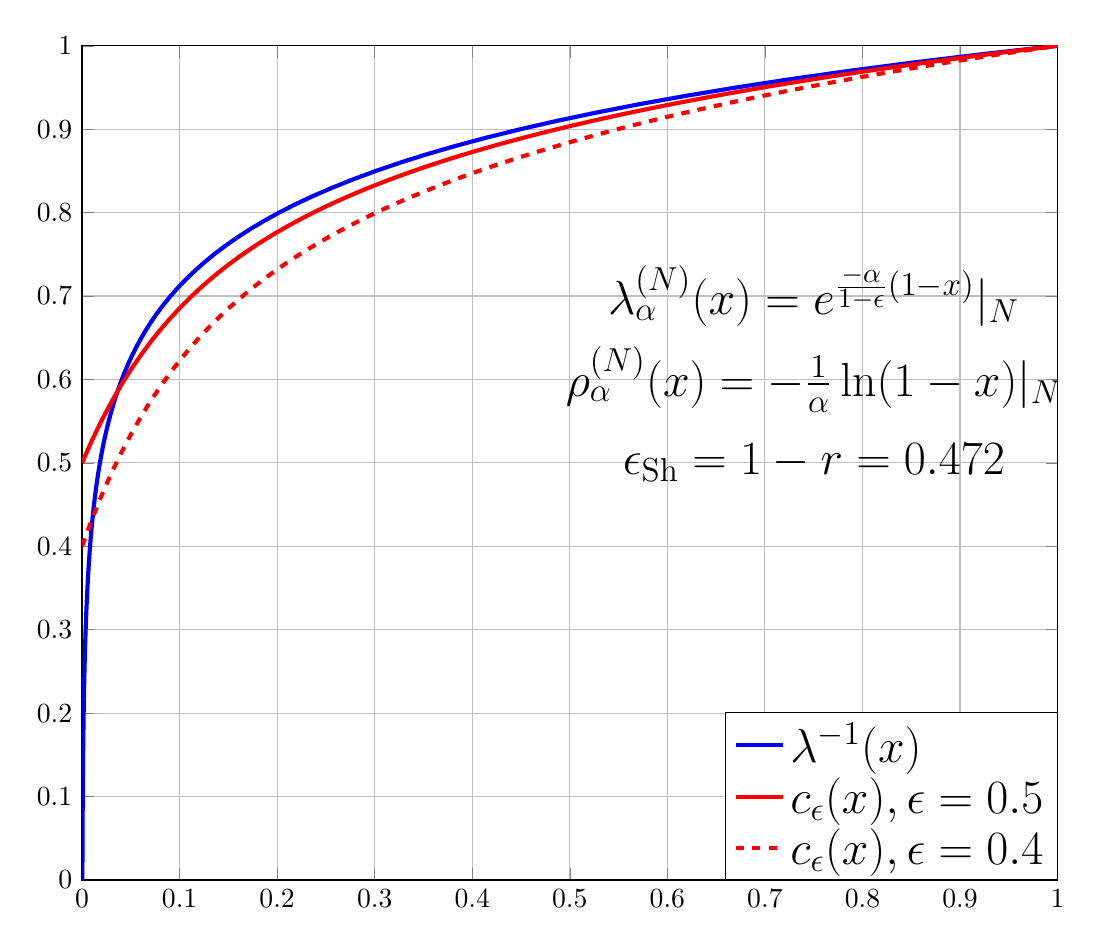
\begin{tikzpicture}
\def\fsize{\LARGE}

\begin{axis}[%
width=4.87804024496938in,
height=4.17068372703412in,
scale only axis,
xmin=0,
xmax=1,
xmajorgrids,
xtick={0,0.1,0.2,...,1},
xticklabels={0,0.1,0.2,0.3,0.4,0.5,0.6,0.7,0.8,0.9,1},
ymin=0,
ymax=1,
legend style={at={(1,0)},anchor=south east,draw=black,fill=white,legend cell align=left,font=\LARGE},
ymajorgrids
]
\node at (axis cs:0.75,0.7){\fsize{$\lambda_{\alpha}^{(N)}(x)=e^{\frac{-\alpha}{1-\epsilon} (1-x)}|_{N}$}};
%\sum\limits_{i=1}^{N}\frac{1}{\alpha}\frac{x^i}{i}}};
\node at (axis cs:0.75,0.6){\fsize{$\rho_{\alpha}^{(N)}(x)=-\frac{1}{\alpha}\ln (1-x)|_{N}$}};
%x^{\frac{1}{\alpha}},\alpha=0.1,N=50$}};
\node at (axis cs:0.75,0.5){\fsize{$\epsilon_{\text{Sh}}=1-r=0.472$}};

\addlegendentry{$\lambda^{-1}(x)$};
\addplot [color=blue,solid,line width=1.5pt]
  table[row sep=crcr]{0.000335494153584825	0\\
0.000363436477858997	0.01\\
0.000393706036385988	0.02\\
0.000426496657682508	0.03\\
0.000462018313674054	0.04\\
0.000500498464232096	0.05\\
0.000542183513693807	0.06\\
0.00058734038869107	0.07\\
0.000636258247392219	0.08\\
0.000689250331101526	0.09\\
0.000746655970072966	0.1\\
0.000808842756382345	0.11\\
0.000876208897771561	0.12\\
0.000949185767537662	0.13\\
0.00102824066679468	0.14\\
0.00111387981679615	0.15\\
0.00120665160047942	0.16\\
0.00130715007398865	0.17\\
0.00141601877066227	0.18\\
0.00153395482184343	0.19\\
0.00166171342090063	0.2\\
0.00180011265904357	0.21\\
0.00195003876389988	0.22\\
0.0021124517743976	0.23\\
0.00228839168829194	0.24\\
0.00247898512170151	0.25\\
0.00268545252329786	0.26\\
0.00290911598934362	0.27\\
0.00315140772962231	0.28\\
0.00341387923847058	0.29\\
0.00369821122963888	0.3\\
0.00400622439859745	0.31\\
0.00433989108120327	0.32\\
0.00470134788338308	0.33\\
0.00509290936270569	0.34\\
0.00551708284945217	0.35\\
0.00597658450208934	0.36\\
0.00647435669995645	0.37\\
0.00701358688453719	0.38\\
0.00759772796996556	0.39\\
0.00823052045346203	0.4\\
0.00891601636728181	0.41\\
0.00965860522554881	0.42\\
0.0104630421321226	0.43\\
0.0113344782294832	0.44\\
0.0122784936836085	0.45\\
0.0133011334160577	0.46\\
0.0144089458120634	0.47\\
0.0156090246524914	0.48\\
0.0169090545381691	0.49\\
0.0183173600974417	0.5\\
0.0198429592920402	0.51\\
0.0214956211625829	0.52\\
0.0232859283834527	0.53\\
0.0252253450275842	0.54\\
0.0273262899750436	0.55\\
0.0296022164354101	0.56\\
0.0320676980931018	0.57\\
0.0347385224271733	0.58\\
0.0376317918030286	0.59\\
0.0407660329832215	0.6\\
0.0441613157583836	0.61\\
0.0478393814576613	0.62\\
0.0518237821612379	0.63\\
0.0561400315059548	0.64\\
0.060815768049174	0.65\\
0.0658809322363014	0.66\\
0.0713679581043317	0.67\\
0.0773119809479292	0.68\\
0.0837510622765184	0.69\\
0.0907264335012647	0.7\\
0.098282759910384	0.71\\
0.106468426620664	0.72\\
0.115335848333247	0.73\\
0.124941804873458	0.74\\
0.135347804658769	0.75\\
0.146620478416798	0.76\\
0.15883200566779	0.77\\
0.172060576694392	0.78\\
0.186390892947055	0.79\\
0.201914709077521	0.8\\
0.218731420056951	0.81\\
0.23694869712112	0.82\\
0.256683176594334	0.83\\
0.278061205978336	0.84\\
0.301219652054399	0.85\\
0.326306776138336	0.86\\
0.353483182051611	0.87\\
0.382922842829663	0.88\\
0.41481421268376	0.89\\
0.449361431268097	0.9\\
0.486785627882633	0.91\\
0.527326333867846	0.92\\
0.571243012123746	0.93\\
0.618816713416241	0.94\\
0.670351869923472	0.95\\
0.726178237327734	0.96\\
0.786652997679963	0.97\\
0.852163036258837	0.98\\
0.923127406721123	0.99\\
1	1\\
};

\addlegendentry{$c_{\epsilon}(x),\epsilon=0.5$};
\addplot [color=red,solid,line width=1.5pt]
  table[row sep=crcr]{0	0.5\\
0.01	0.526526126042806\\
0.02	0.550706243040251\\
0.03	0.57280262188789\\
0.04	0.593046195873519\\
0.05	0.6116403489369\\
0.06	0.628764252863599\\
0.07	0.644575805441883\\
0.08	0.659214215869252\\
0.09	0.672802278552915\\
0.1	0.685448371847462\\
0.11	0.697248214159826\\
0.12	0.708286406177705\\
0.13	0.718637784699063\\
0.14	0.728368610616949\\
0.15	0.73753761100972\\
0.16	0.746196892968877\\
0.17	0.754392744735548\\
0.18	0.762166337885451\\
0.19	0.769554342676617\\
0.2	0.776589467232609\\
0.21	0.783300929956643\\
0.22	0.789714873441285\\
0.23	0.795854727138328\\
0.24	0.801741525169708\\
0.25	0.807394184880162\\
0.26	0.812829751044085\\
0.27	0.818063610032608\\
0.28	0.82310967771285\\
0.29	0.827980564381521\\
0.3	0.832687719622072\\
0.31	0.837241559611941\\
0.32	0.841651579088144\\
0.33	0.84592644990045\\
0.34	0.850074107836845\\
0.35	0.854101829192009\\
0.36	0.858016298362217\\
0.37	0.861823667586471\\
0.38	0.865529609810601\\
0.39	0.869139365526266\\
0.4	0.87265778432787\\
0.41	0.876089361835362\\
0.42	0.879438272548156\\
0.43	0.882708399123219\\
0.44	0.885903358507587\\
0.45	0.889026525300862\\
0.46	0.892081052675632\\
0.47	0.89506989114236\\
0.48	0.897995805409208\\
0.49	0.900861389555933\\
0.5	0.903669080713676\\
0.51	0.906421171418762\\
0.52	0.909119820787906\\
0.53	0.911767064644275\\
0.54	0.914364824708154\\
0.55	0.91691491695232\\
0.56	0.919419059210307\\
0.57	0.921878878115366\\
0.58	0.924295915438839\\
0.59	0.926671633888754\\
0.6	0.929007422422485\\
0.61	0.931304601121274\\
0.62	0.93356442566907\\
0.63	0.935788091473473\\
0.64	0.937976737462459\\
0.65	0.94013144958696\\
0.66	0.94225326405617\\
0.67	0.944343170329661\\
0.68	0.946402113887892\\
0.69	0.948430998800506\\
0.7	0.950430690109856\\
0.71	0.952402016045493\\
0.72	0.954345770083781\\
0.73	0.95626271286546\\
0.74	0.958153573982763\\
0.75	0.960019053646566\\
0.76	0.961859824243142\\
0.77	0.963676531789142\\
0.78	0.965469797292704\\
0.79	0.967240218027864\\
0.8	0.968988368728802\\
0.81	0.970714802709912\\
0.82	0.972420052917143\\
0.83	0.974104632915626\\
0.84	0.97576903781815\\
0.85	0.977413745158703\\
0.86	0.979039215714913\\
0.87	0.980645894282958\\
0.88	0.982234210408185\\
0.89	0.983804579074453\\
0.9	0.985357401354956\\
0.91	0.986893065027096\\
0.92	0.988411945153746\\
0.93	0.989914404633095\\
0.94	0.991400794719091\\
0.95	0.992871455514339\\
0.96	0.994326716437194\\
0.97	0.995766896664656\\
0.98	0.997192305552543\\
0.99	0.998603243034339\\
1	1\\
};

\addlegendentry{$c_{\epsilon}(x),\epsilon=0.4$};
\addplot [color=red,dashed,line width=1.5pt]
  table[row sep=crcr]{0	0.4\\
0.01	0.431831351251367\\
0.02	0.460847491648301\\
0.03	0.487363146265468\\
0.04	0.511655435048223\\
0.05	0.533968418724279\\
0.06	0.554517103436319\\
0.07	0.57349096653026\\
0.08	0.591057059043103\\
0.09	0.607362734263498\\
0.1	0.622538046216955\\
0.11	0.63669785699179\\
0.12	0.649943687413245\\
0.13	0.662365341638875\\
0.14	0.674042332740338\\
0.15	0.685045133211665\\
0.16	0.695436271562653\\
0.17	0.705271293682658\\
0.18	0.714599605462541\\
0.19	0.723465211211941\\
0.2	0.731907360679131\\
0.21	0.739961115947971\\
0.22	0.747657848129542\\
0.23	0.755025672565993\\
0.24	0.76208983020365\\
0.25	0.768873021856194\\
0.26	0.775395701252902\\
0.27	0.781676332039129\\
0.28	0.78773161325542\\
0.29	0.793576677257825\\
0.3	0.799225263546487\\
0.31	0.804689871534329\\
0.32	0.809981894905773\\
0.33	0.81511173988054\\
0.34	0.820088929404215\\
0.35	0.82492219503041\\
0.36	0.82961955803466\\
0.37	0.834188401103766\\
0.38	0.838635531772721\\
0.39	0.84296723863152\\
0.4	0.847189341193444\\
0.41	0.851307234202435\\
0.42	0.855325927057787\\
0.43	0.859250078947862\\
0.44	0.863084030209105\\
0.45	0.866831830361034\\
0.46	0.870497263210758\\
0.47	0.874083869370832\\
0.48	0.87759496649105\\
0.49	0.881033667467119\\
0.5	0.884402896856411\\
0.51	0.887705405702515\\
0.52	0.890943784945487\\
0.53	0.89412047757313\\
0.54	0.897237789649784\\
0.55	0.900297900342784\\
0.56	0.903302871052369\\
0.57	0.906254653738439\\
0.58	0.909155098526607\\
0.59	0.912005960666505\\
0.6	0.914808906906982\\
0.61	0.917565521345529\\
0.62	0.920277310802884\\
0.63	0.922945709768168\\
0.64	0.925572084954951\\
0.65	0.928157739504352\\
0.66	0.930703916867404\\
0.67	0.933211804395593\\
0.68	0.935682536665471\\
0.69	0.938117198560607\\
0.7	0.940516828131827\\
0.71	0.942882419254591\\
0.72	0.945214924100537\\
0.73	0.947515255438552\\
0.74	0.949784288779315\\
0.75	0.952022864375879\\
0.76	0.954231789091771\\
0.77	0.95641183814697\\
0.78	0.958563756751245\\
0.79	0.960688261633437\\
0.8	0.962786042474563\\
0.81	0.964857763251894\\
0.82	0.966904063500572\\
0.83	0.968925559498751\\
0.84	0.970922845381781\\
0.85	0.972896494190444\\
0.86	0.974847058857895\\
0.87	0.976775073139549\\
0.88	0.978681052489822\\
0.89	0.980565494889343\\
0.9	0.982428881625947\\
0.91	0.984271678032515\\
0.92	0.986094334184495\\
0.93	0.987897285559714\\
0.94	0.98968095366291\\
0.95	0.991445746617207\\
0.96	0.993192059724633\\
0.97	0.994920275997587\\
0.98	0.996630766663051\\
0.99	0.998323891641207\\
1	1\\
};
\end{axis}
\end{tikzpicture}}
  %\includegraphics[width=2.2in]{./Figures/EXIT_PoissSoliton}
\end{center}
\column{0.45\textwidth}
\begin{center}
  \includegraphics[width=2.2in]{./Figures/ratelesserasures3}
\end{center}
\end{columns}
%\begin{block}{Poisson, Soliton pair is optimal - $\lambda(x) = e^{-r_{avg}(1-x)}$}
\begin{itemize}
%\item Poisson, soliton pair is optimal
  %\item Left degree is Poisson : $\lambda(x) = e^{-r_{avg}(1-x)}$
  \item   $x = \lambda(1-(1-\epsilon)\rho(1-x))$
  \item $\lambda(x) = e^{-\frac{\alpha}{1-\epsilon}(1-x)}$, \alert{optimal right degree is soliton: $\rho(x) = -\frac{1}{\alpha}\ln(1-x)$}
  %\item \alert{Optimal distribution is soliton: $f_D[i] = \frac{1}{i(i-1)}$}
\end{itemize}
\begin{center}
\begin{tabular}{|l|c|c|c|c|c|c|c|c|}
\hline
Degree of nodes & 1 & 2 & 3 & 4 & $\ldots$ & $i$ & \ldots & $K$ \\
\hline
Fraction: \alert{ $f_D[i]$ } & $\frac{1}{K}$ & $\frac12$ & $\frac16$ & $\frac{1}{12}$ & $\ldots$ & $\frac{1}{i(i-1)}$ & \ldots & $\frac{1}{K (K-1)}$ \\
\hline
\end{tabular}
\end{center}
%\end{block}
\end{frame}
%------------------------------------------------------------------------------------
\begin{frame}{Connection with Luby Transform (LT) codes}
%\begin{columns}
%\begin{column}{0.47\textwidth}
%\begin{center}
%\includegraphics[width=1.5in]{../../Projects/MACcollision/Figures/poissonapproxerasures}
%\end{center}
%\end{column}
%\begin{column}{0.47\textwidth}
%\begin{center}
%\includegraphics[width=2.0in]{../../Projects/MACcollision/Figures/ratelesserasures}
%\end{center}
%\end{column}
%\end{columns}
\begin{center}
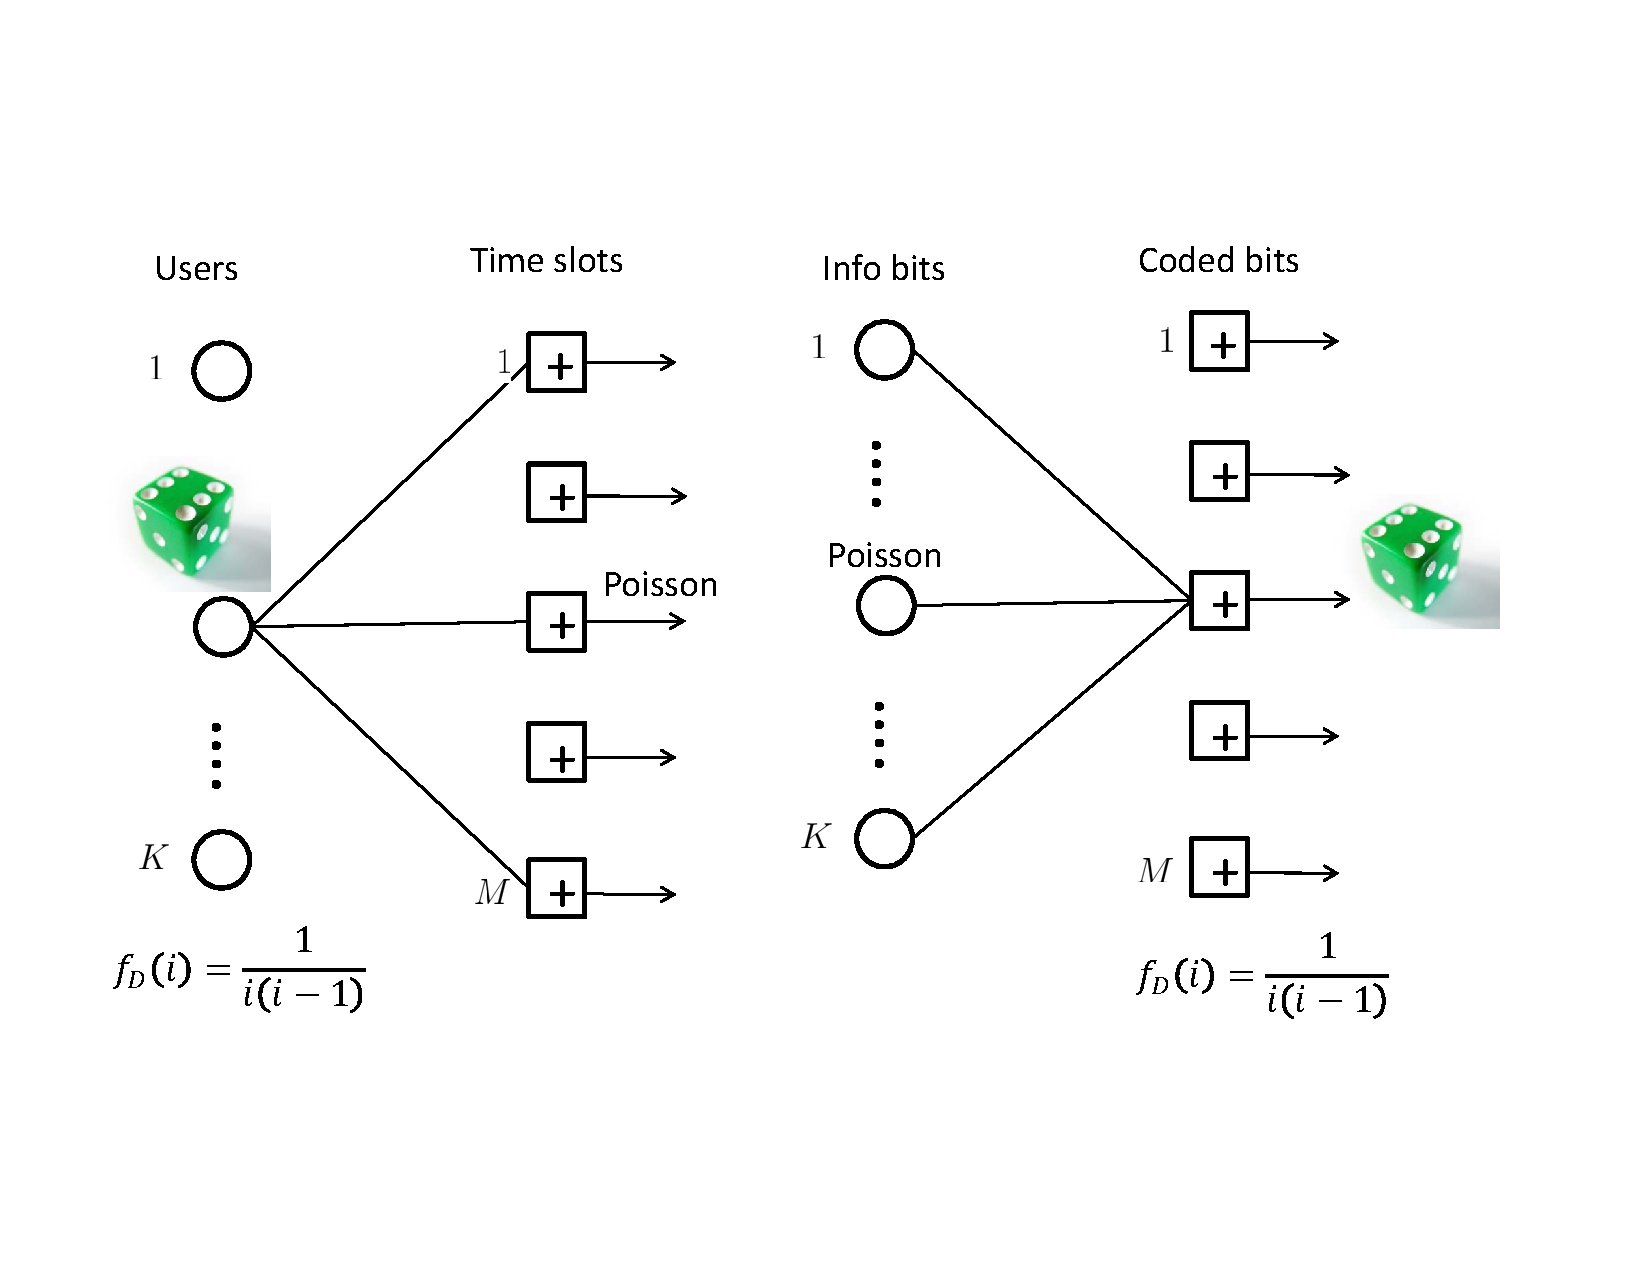
\includegraphics[width=3.8in]{./Figures/ratelessmaccomparison}
\end{center}
\begin{itemize}
  \item For rateless codes $\lambda(x)$ is Poisson and $\rho(x)$ is soliton
  \item For multiple access $\rho(x)$ is Poisson, \alert{optimal $\lambda(x)$ is soliton}
  \item Our result shows that both are optimal pairs
\end{itemize}
\end{frame}
%%--------------------------------------------------------------------------------------
%\begin{frame}{Histogram of required $N$ for $K=10000$}
%\begin{center}
%  \includegraphics[width=4.2in]{./Figures/fountaincodes10000histogram}
%\end{center}
%\begin{block}{Finite length considerations}
%\begin{itemize}
%  \item Deg. dist. must be adjusted for optimizing finite length performance
%  \item Raptor codes (Shokrollahi'06) is an excellent choice
%\end{itemize}
%\end{block}
%\end{frame}
%------------------------------------------------------------------------------------
%\begin{frame}{Asymptotic decoding analysis}
%\begin{itemize}
%\item Analyze the ensemble $\mathcal{G}(K,M,\lambda,\rho)$ in the limit as $K,M \rightarrow \infty$
%\item ${\sf x}_\ell$ - prob. outgoing msg from var node is erased ($\ell$-th iteration)
%\item ${\sf y}_\ell$ - prob. outgoing msg from check node is erased ($\ell$-th iteration)
%\end{itemize}
%\begin{center}
%\includegraphics[width=4.0in]{../Figures/graphicalmodelDE}
%\end{center}
%\end{frame}
%%------------------------------------------------------------------------------------
%\begin{frame}{Decoding analysis - Density evolution}
%\begin{columns}
%\begin{column}{0.4\textwidth}
%\begin{center}
%\includegraphics[width=1.6in]{../Figures/leftnode}
%\end{center}
%\small
%\begin{eqnarray}
%\nonumber x_{l,i} & = & y_l^{i-1} \\
%\nonumber x_l & = & \sum_i \lambda_i y_l^{i-1} = \lambda(y_l)
%\end{eqnarray}
%\end{column}
%\pause
%\begin{column}{0.57\textwidth}
%\begin{center}
%\includegraphics[width=1.6in]{../Figures/rightnode}
%\end{center}
%\small
%\begin{eqnarray}
%\nonumber y_{l+1,j} & = & 1-(1-x_l)^{j-1} \\
%\nonumber y_{l+1} & = & \sum_j \rho_j (1-(1-x_l)^{j-1}) = 1 - \rho(1-x_l)
%\end{eqnarray}
%\end{column}
%\end{columns}
%\end{frame}
%------------------------------------------------------------------------------------
%\normalsize
%\begin{frame}{Density evolution and successful decoding}
%\begin{columns}
%\begin{column}{0.47\textwidth}
%\begin{center}
%\includegraphics[width=1.0in]{../Figures/leftnode}
%\end{center}
%\end{column}
%\pause
%\begin{column}{0.47\textwidth}
%\begin{center}
%\includegraphics[width=1.0in]{../Figures/rightnode}
%\end{center}
%\end{column}
%\end{columns}
%\begin{block}{Density evolution}
%\vspace{-5mm}
%\begin{align*}
%{\sf x}_0 & = 1\\
%\nonumber
%{\sf y}_{\ell+1} & = 1 - \rho(1-{\sf x}_\ell) \\
%\nonumber
%{\sf x}_\ell & = \lambda({\sf y}_{\ell}) \\
%\nonumber
%{\sf y}_{\ell+1} & =  1 - \rho \left( (1-\lambda({\sf y}_{\ell}) \right)
%\end{align*}
%\end{block}
%\pause
%\begin{block}{Successful decoding condition}
%\[
%\boxed{\rho(1-\lambda(y)) > 1-y, \ \ \ y \in (0,1-\rho(0)]}
%\]
%\end{block}
%\end{frame}
%------------------------------------------------------------------------------------
\iffalse
\begin{frame}

\begin{block}{Successful decoding}
\[
\rho(1-\lambda(y)) > 1-y, \ \ \ y \in (0,1-\rho(0)]
\]
\end{block}

\begin{block}{Stability condition}
Checking the derivative of this condition at $y=0$ gives the \emph{stability condition}, $\lambda_2 \rho'(1) \leq 1$, which is also required for convergence to 0. If the inequality is strict, then $y_\ell$ converges to 0 exponentially with iteration for sufficiently large $l$.
\end{block}

\end{frame}
\fi
%%------------------------------------------------------------------------------------
%\begin{frame}{Graphical interpretation - EXIT chart}
%\begin{center}
%\includegraphics[width=3.5in]{../Figures/DEregular1}
%\end{center}
%\end{frame}
%%------------------------------------------------------------------------------------
%\begin{frame}{Graphical interpretation - EXIT chart}
%\begin{center}
%\includegraphics[width=3.5in]{../Figures/DEregular2}
%\end{center}
%\end{frame}
%------------------------------------------------------------------------------------
%\begin{frame}{Intuition behind the main result}
%%\small
%\begin{block}{Convergence follows from $\rho(1-\lambda(y)) > 1-y$}
%\begin{align*}
%\rho(1-\lambda(y)) &= 1-y \\
%e^{-\texttt{r}_{avg} \lambda(y)} &= e^{\ln(1-y)}\\
%\Rightarrow -\texttt{r}_{avg} \lambda(y)&= \ln(1-y) = -\sum_{i=1}^{\infty} \frac{y^i}{i}\\
%\Rightarrow \texttt{r}_{avg} \sum_i \lambda_i y^i & = \sum_{i=1}^{\infty} \frac{y^i}{i}
%\end{align*}
%\end{block}
%%\begin{itemize}
%%\item Analyze numerator of $\lambda^N(x)$ using $-\ln(1-x) = \sum_{i=1}^{\infty} \frac{x^i}{i}$
%%\item For $y\in(0,1)$, $-ay + \sum_{i=1}^{N} \frac{y^i}{i} < -ay -\ln(1-y)$
%%\item $\rho^N(1-\lambda^N(y)) = e^{ay-\sum_{i=1}^N \frac{y^i}{i}} > e^{\ln(1-y)} e^{ay} > (1-y)$
%%\end{itemize}
%%\end{block}
%%\vspace{-1mm}
%\pause
%\begin{block}{}
%\begin{align*}
%\texttt{r}_{avg} \lambda_i &= \frac{1}{i}\\
%\sum_i \lambda_i & = 1 \Rightarrow \boxed{\texttt{r}_{avg} = \sum_i \frac{1}{i}, \lambda_i = \frac{1/i}{\sum_i 1/i}} \Rightarrow \boxed{L_i = \frac{1}{i(i-1)}, i\geq2}
%\end{align*}
%\end{block}
%\end{frame}
%%-------------------------------------------------------------------------------------
%\begin{frame}{Precise proof}
%\begin{block}{Truncate and adjust}
%\begin{itemize}
%\item Consider $\lambda^N(x) =  \frac{L'^N(x)}{L'^N(1)} = \frac{\sum_{i=1}^{N}\frac{x^i}{i}-ax}{H(N)-a}, \ \ \rho(x) = e^{-(H(N)-a)(1-x)}$
%\item $H(N) = \sum_{i=1}^N \frac{1}{i}$
%\end{itemize}
%\end{block}
%\begin{block}{Efficiency}
%\vspace{-6mm}
%\begin{align*}
%\eta^N & = \frac{R'^N(1)}{L'^N(1)} = \frac{H(N)-a}{\frac{H(N)-a}{\sum_{i=2}^{N+1} \frac{1}{i(i-1)}-a}}
%\nonumber
%= \sum_{i=1}^{N} \frac{1}{i(i+1)}  - a = \frac{N}{N+1} - a
%\end{align*}
%\end{block}
%
%\pause
%\vspace{-6mm}
%\begin{block}{Stability}
%\begin{itemize}
%\item Expand $1-\rho(1-\lambda({\sf y}_\ell))$ around $\sf{y}_\ell = 0$ to get \vspace*{-2mm}
%\[ {\sf y}_{\ell+1} = \lambda_2^N \rho'^N(1) {\sf y}_\ell + O({\sf y}^2_\ell) = (1-a)  {\sf y}_\ell + O({\sf y}^2_\ell) \]
%%\item For any $a >  0$, the stability condition is satisfied
%\end{itemize}
%\end{block}
%\end{frame}
%---------------------------------------------------------------------------------------------------
%\begin{frame}{Precise result}
%\vspace{-4mm}
%%\begin{itemize}
%%\item Soliton distribution,  $L(x) = \sum_{i=2}^{\infty} \frac{x^i}{i(i-1)}$, is optimal
%%\end{itemize}
%%\pause
% \begin{block}{}
% {Theorem: For any $a\in[0,1]$, consider the sequence (indexed by $N\in \mathbb{N}$) of node-perspective degree-distributions,  $(L^N(x),R^N(x))$, where
%\begin{align*}
%L^N(x) &= \frac{\sum_{i=2}^{N+1}\frac{x^i}{i(i-1)}-\frac{a x^2}{2}}{\sum_{i=2}^{N+1}\frac{1}{i(i-1)}-\frac{a}{2}} \\
%R^N(x) &= e^{-\left(H(N)-a\right)(1-x)}.
%\end{align*}
%Here $H(N) = \sum_{i=1}^N \frac{1}{i}$ is the $N$-th Harmonic number. For every ensemble in this sequence, ${\sf y}_\ell \stackrel{\ell \rightarrow \infty}{\rightarrow} 0$ while $\eta^N = \frac{N}{N+1} - a \stackrel{N \rightarrow \infty}{\rightarrow} 1-a$.}
%\end{block}
%%\vspace{2mm}
%%\alert{Stability:} For any $a>0$, the stability condition is strictly satisfied
%
%\begin{block}{}
%For $\eta \rightarrow 1$, $\texttt{r}_{avg} \rightarrow \infty \Rightarrow P$(right degree $=1) \rightarrow 0$
%\end{block}
%\end{frame}
%------------------------------------------------------------------------------------
\begin{frame}{Simulation Results}
\begin{center}
\includegraphics[width=3.2in]{C:/Users/nrkri/Dropbox/Work/RESEARCH/Projects/MACcollision/Figures/Simulationresultserasure}
\end{center}
\begin{itemize}
\item Even for $K=10000$, efficiency close to 0.8 can be obtained
\end{itemize}
\end{frame}
%------------------------------------------------------------------------------------
\begin{frame}{Some open problems}
\begin{itemize}
\item Fundamental limits on universal multiple access, i.e. $K$, $\epsilon$ not known
\item Uncoordinated multiple access with power constraint and Gaussian noise
    \begin{itemize}
    \item Power penalty for repeating information $\log n$ times on the average
    \item Can we achieve the equal rate point on the MAC region with simple decoding?
    \end{itemize}
\end{itemize}
\end{frame}
%------------------------------------------------------------------------------------
%\begin{frame}{Average Degree and its Consequences}
%\begin{block}{Optimal distribution is soliton: $f(i) = \frac{1}{i(i-1)}$}
%\begin{center}
%\begin{tabular}{|l|c|c|c|c|c|c|}
%\hline
%No. of times & 1 & 2 & 3 & 4 & $\ldots$ & $M$ \\
%\hline
%Fraction of users & 0 & $\frac12$ & $\frac16$ & $\frac{1}{12}$ & $\ldots$ & $\frac{1}{M (M-1)}$ \\
%\hline
%\end{tabular}
%\end{center}
%\end{block}
%\begin{block}{Average degree}
%\begin{itemize}
%\item Average left degree is $\ln M \Rightarrow $ average right degree is $\eta \ln M$
%\item For $K,M \rightarrow \infty$, $\texttt{r}_{avg} \rightarrow \infty \Rightarrow P$(right degree $=1) \rightarrow 0$
%\end{itemize}
%\end{block}
%\pause
%\begin{block}{Consequences}
%\begin{itemize}
%\item Consequence 1: Iterations can get stuck at the beginning
%\item Consequence 2: Average power consumed is $\ln K$ times larger
%\item Data is not centrally available - joint precoding is not an option
%\end{itemize}
%\end{block}
%\end{frame}
%\begin{frame}{Non-Asymptotic Regime - Non-Poisson Right degrees?}
%%\vspace{-2mm}
%\begin{itemize}
%\item For fixed number of users $K$, is this scheme still the optimal thing to do?
%\item<2-> Each user picks the time-slots uniformly at random (uniform PMF)
%\item<2-> What about other PMFs?
%\item<2-> By picking step like PMF, we can induce mixture of Poisson distributions
%\end{itemize}
%\pause
%\begin{figure}
%\input{../Figures/PMFs_Uniform_Steplike.tex}
%\end{figure}
%\end{frame}

%\begin{frame}{Simulation Results, $K = 1000$}
%\begin{figure}
%\input{../../Projects/MACcollision/Figures/BERvsEfficiency.tex}
%\end{figure}
%\end{frame}

%\begin{frame}{Analysis of Peeling Decoder}
%\begin{itemize}
%\item Uniform leads to $\rho(x)$ =Poisson distribution, step-like PMF results in mixture of two Poisson PMFs.
%\item $\rho_{1}$ for Poisson mixture is higher thus a lower probability of peeling decoder getting stuck in the initial stages.
%\end{itemize}
%\begin{figure}
%\input{../Figures/ResidualGraph_Degree1Nodes.tex}
%\caption{Expected path in the residual graph of peeling decoder}
%\end{figure}
%\end{frame}

%\begin{frame}{Back to theory: from erasures to errors}
\end{frame}
%-----------------------------------------------------------------------
\begin{frame}\frametitle{Finite field with $p$ elements}
\begin{block}{$p$ is prime}
\begin{itemize}
\item $\mathbb{F}_p - \{0,1,2,\ldots,p-1\}$
\item $a \oplus b = (a+b) \mod p$
\item $a \odot b = (ab) \mod p$
\item We can $+,\times,\div$, inverses
\item $W$ is a (primitive) element such that $1,W,W^2,\ldots,W^{p-1}$ are distinct
\end{itemize}
\end{block}
\pause
\begin{block}{Example $\mathbb{F}_5$}
\begin{itemize}
\item $W=2$
\item $W^0=1, W^1=2, W^2 = 4, W^3 = 3$
\end{itemize}
\end{block}
\pause
\begin{block}{$p$ need not be prime}
\begin{itemize}
\item Everything can be extended to finite fields with $q = 2^r$ elements
\item May be extended to integers - not sure
\end{itemize}
\end{block}
\end{frame}
%-------------------------------------------------------------
\begin{frame}{$p$-symmetric channel and error correction}

\begin{figure}[t]
\centering
\scalebox{0.55}{%\documentclass{article}
%
%\usepackage{tikz}
%\usetikzlibrary{arrows,shapes,chains,matrix,positioning,scopes,patterns,calc}
%\usepackage{color}
%
%\usepackage{latexsym}
%\usepackage{amsmath,amssymb,amsthm}
%\usepackage{etoolbox}
%
%\begin{document}

\begin{tikzpicture}
\def \recW{1in}; %Encoder Length
\def \recH{0.5in}; %Encoder Width

\def \R{0.06in}; %Larger circle radius

\def \Gblks{0.25in}; %Gaps between blocks
\def \ext{0.95in}; %Extensions towards left and right of the figure
\def \extB{0.25in}; %Extensions towards top of the figure

\def \fsizes{\normalsize}; %Defining a generic font size to be adjusted depending on the scaling
\def \fsize{\Large}; %Defining a generic font size to be adjusted depending on the scaling

\tikzstyle{rect}   = [ rectangle, draw, text centered, thick,
                        minimum height=\recH, minimum width=\recW ]

\node [rect](enc) at (0,0) {\fsizes{Encoder}} ;
\node (chan)  [right = \ext of enc,draw,rectangle,text centered,thick,minimum width=1.5in,minimum height=1.5in]    {\includegraphics[width=1.5in,height=1.5in,angle=-90]{Parysymmetricchannelmodel.pdf}};
\node (dec)[rect,right=\ext of chan] {\fsizes Decoder} ;

\draw[<-,thick](enc)-- +(-2*\ext,0) node[midway,above]{\fsize $m_1,\ldots,m_k$};
\draw[->,thick](enc)--(chan)node[midway,above]{\fsize $x_1,\ldots,x_n$}node[midway,below]{\fsize $x_i\in \mathbb{F}_p$};
\draw[->,thick](chan)--(dec)node[midway,above]{\fsize $r_1,\ldots,r_n$}node[midway,below]{\fsize $r_i\in \mathbb{F}_p$};;

%\draw[<-,thick](chan)--+(0,\extB) node[above] {\fsize $e_1,\ldots,e_n$};
\draw[->,thick](dec)--+(2*\ext,0)node[midway,above]{\fsize  $\hat{m_1},\ldots,\hat{m_k}$};

\end{tikzpicture}
%\end{document} }
\end{figure}

\begin{block}{Error correction coding}
\begin{itemize}
%\item Capacity $C = 1-H_2(\epsilon)$
\item Another simple channel model which has been extensively considered
\item Has been the canonical model for algebraic coding theorists
\end{itemize}
\end{block}
%\vspace*{-5mm}
%\begin{figure}[t]
%\centering
%\includegraphics[width=1.5in,angle=-90]{./Figures/Parysymmetricchannelmodel}
%\end{figure}
\end{frame}

%--------------------------------------------------------------------------------------
\begin{frame}{Generalized LDPC code and error channels}
\vspace{-7mm}
\begin{figure}[t]
\centering
\includegraphics[width=2.15in,angle=-90]{./Figures/GLDPC}
\end{figure}

\begin{block}{}
\begin{itemize}
\item GLDPC introduced by Tanner in 1981
\item Each check is a $(\tilde{n},\tilde{k})$, $t$-error correcting code
\item If there are $\leq t$ errors in a check, it can be recovered
%\item Density evolution equations can be written and thresholds computed
\item For now, assume no miscorrections
\end{itemize}
\end{block}
\end{frame}
%--------------------------------------------------------------------------------------
\begin{frame}{Peeling process is same for erasure and error channels}
\begin{columns}
\column{0.5\textwidth}
\includegraphics[width=2.3in,angle=-90]{./Figures/Tannergraph63codewitherasures}
\column{0.5\textwidth}
\includegraphics[width=2.15in,angle=-90]{./Figures/GLDPC}
\end{columns}
\begin{block}{}
\begin{itemize}
  \item Assume 1-error correcting check code and no miscorrections
  \item One-to-one correspondence between messages passed - DE can be used
  \item Not optimal for the error channel but it is not bad at high rates
  \item Spatially coupled versions are optimal at high rates (Jian, Pfister and N)
\end{itemize}
\end{block}
\end{frame}
%--------------------------------------------------------------------------------------
\begin{frame}\frametitle{Erasures to errors - tensoring and peeling}
\begin{columns}
    \column{.45\textwidth}
    \small
    \[
    H = \left[
    \begin{array}{ccccccc}
    1&0&1&1&0&0\\
    1&1&0&0&1&0 \\
    0&1&1&0&0&1
    \end{array}
    \right]
    \]
    \[
    \otimes
    \]
    \[
    B = \left[
    \begin{array}{ccccccc}
    1&1&1&1&1&1\\
    1&W&W^2&W^3&W^4&W^5
    \end{array}
    \right]
    \]
    \[
    \mathbf{\tilde{H}} = \left[
    \begin{array}{ccccccc}
    1&0&1&1&0&0\\
    1&0&W^2&W^3&0&0\\
    1&1&0&0&1&0 \\
    1&W&0&0&W^4&0 \\
    0&1&1&0&0&1 \\
    0&W&W^2&0&0&W^5
    \end{array}
    \right]
    \]
    \column{.45\textwidth}
    \begin{figure}[t]
    \centering
    \includegraphics[width=2.0in,angle=-90]{./Figures/GLDPC}
    \end{figure}
\end{columns}
\begin{block}{}
\begin{itemize}
\item $W$ is a primitive element in the field
\item Each check is a 1-error correcting code
\item If there is exactly one error in a check, it can be recovered
\end{itemize}
\end{block}
\end{frame}
%%--------------------------------------------------------------------------------------
%\begin{frame}{Generalized LDPC Code}
%
%\begin{columns}
%    \column{.6\textwidth}
%    .
%%    \small
%%    \[
%%    H = \left[
%%    \begin{array}{ccccccc}
%%    1&0&1&1&0&0\\
%%    1&1&0&0&1&0 \\
%%    0&1&1&0&0&1
%%    \end{array}
%%    \right]
%%    \]
%%    \[
%%    \otimes
%%    \]
%%    \[
%%    T = \left[
%%    \begin{array}{ccccccc}
%%    1&1&1&1&1&1\\
%%    1&W&W^2&W^3&W^4&W^5 \\
%%    \vdots & \vdots & \vdots & \vdots & \vdots & \vdots \\
%%    1&W^{2t-1}&W^{2(2t-1)}&\cdots&\cdots&W^{5(2t-1)}
%%    \end{array}
%%    \right]
%%    \]
%%    \[
%%    \mathbf{\tilde{H}} = H \otimes T
%%    \]
%    \column{.4\textwidth}
%    \begin{figure}[t]
%    \centering
%    \includegraphics[width=2.0in,angle=-90]{./Figures/GLDPC}
%    \end{figure}
%\end{columns}
%
%\begin{itemize}
%\item GLDPC introduced by Tanner in 1981
%\item Each check is a $t$-error correcting code
%\item If there are exactly $t$ errors in a check, it can be recovered
%\item Density evolution equations can be written and thresholds computed
%\end{itemize}
%
%\end{frame}

%--------------------------------------------------------------------------------------
\begin{frame}{Product code}
\begin{itemize}
\item Special case of generalized LDPC code
\item Let component code $\mathcal{C}$ be an $(\tilde{n},\tilde{k},\tilde{d}_{\text{min}})$ linear code
\item Well-known that \textcolor{blue}{$\mathcal{P}$ is an $(\tilde{n}^{2},\tilde{k}^{2},\tilde{d}_{\text{min}}^{2})$
linear code }
\end{itemize}

\begin{center}
\scalebox{0.8}{\tikzset
{
    vnodeStyle/.style =
    {
        % -- shape properties --
        circle,                                 % shape
        minimum size    = 7mm,                %
        scale           = 1.0,                  % scaling factor
        thick,                                  % thickness of the border
        %
        % -- colours properties --
        % filling: [ trasparent | monocolored | shaded]; decomment what you prefer
%       %                                       % transparent (all commented)
        fill            = yellow!10,             % monocolored
        text            = black,                % colour of the fonts
        draw            = black,                % colour of the border
        %
        % -- fonts --
        font            = \scriptsize,              % shape of the font (or dimension, like \tiny)
%       text centered,                          % text alignment [text centered | text badly centered | text justified | text ragged | text badly ragged]
        inner xsep      = 0mm,                  % minimum distance between text and borders along x dimension
        inner ysep      = 0mm,                  % minimum distance between text and borders along y dimension
        text height     = 0.2cm,
        text depth      = 0.12cm,
    }
}

%\begin{center}
\tikzstyle{styB}=[circle,
  ball color=blue,
  inner sep=0pt,
  minimum size=10pt]
\tikzstyle{styKB}=[circle,
  ball color=blue!10!white,
  inner sep=0pt,
  minimum size=10pt]
\tikzstyle{styCd}=[rectangle, draw=blue!50,
  top color=blue!40!white, bottom color=blue!10,
  inner sep=0pt,
  minimum size=10pt]
\tikzstyle{styCu}=[rectangle, draw=blue,
  top color=blue, bottom color=blue!40,
  inner sep=0pt,
  minimum size=10pt]

\pgfdeclarelayer{background}
%
\pgfdeclarelayer{foreground}
%
\pgfdeclarelayer{m-f}
%
\pgfdeclarelayer{main}
%
\pgfsetlayers{background,main,m-f,foreground}

\begin{tikzpicture}[scale=2.0]
% \draw[step=5mm,color=gray!40!white, thin] (0,0) grid (12,5);

\colorlet{uecolr}{black} \colorlet{decolr}{black!40}

\def\strt  {-40mm}
\def\shf   {10mm}
\def\ang   {55}
\def\dist  {4mm}
\def\cvd   {18mm}

\def\n     {6}
\def\s     {7}

\begin{scope}[xshift=-7cm, yshift=-1.2cm]

\only<1>
{
%\node (cc) at (12mm,5mm) {Product Code\vphantom{y}};

\foreach \rr in {0,1,...,\n}
 \foreach \cc in {0,1,...,\n}
  \node[vnodeStyle] (p\rr\cc) at (\rr*4mm,-\cc*4mm) {$X_{\cc,\rr}$};

 \node [rectangle,rounded corners=2mm,minimum width=7mm,minimum height=55mm,draw=red,thick] (circ1) at (4mm,-12mm) {};
 \node [rectangle,rounded corners=2mm,minimum width=55mm,minimum height=7mm,draw=red,thick] (circ2) at (12mm,-4mm) {};
}

\only<2>
{
%\node (cc) at (12mm,5mm) {Product Code\vphantom{y}};

\foreach \rr in {0,1,...,\n}
 \foreach \cc in {0,1,...,\n}
  \node[vnodeStyle] (p\rr\cc) at (\rr*4mm,-\cc*4mm) {$X_{\cc,\rr}$};

 \node [rectangle,rounded corners=2mm,minimum width=39mm,minimum height=39mm,draw=black,thick] (circ1) at (8mm,-8mm) {};
 \node [rectangle,rounded corners=2mm,minimum width=14mm,minimum height=55mm,draw=blue,thick] (circ1) at (22mm,-12mm) {};
 \node [rectangle,rounded corners=2mm,minimum width=55mm,minimum height=14mm,draw=red,thick] (circ2) at (12mm,-22mm) {};
}

%\only<2>
%{
%\node (cc) at (12mm,5mm) {Symmetric Subcode};
%
%\foreach \cc in {0,1,...,\n}
%  \foreach \rr in {\cc,...,\n}
%    \node[vnodeStyle] (p\rr\cc) at (\rr*4mm,-\cc*4mm) {$X_{\cc,\rr}$};
%
%\pgfmathtruncatemacro{\nnn}{\n-1}
%\foreach \rr in {0,1,...,\nnn} {
%  \pgfmathtruncatemacro{\rrr}{\rr+1}
%  \foreach \cc in {\rrr,...,\n}
%    \node[vnodeStyle] (p\rr\cc) at (\rr*4mm,-\cc*4mm) {$X_{\color{red}{\rr,\cc}}$};
%}
%
% \node [rectangle,rounded corners=2mm,minimum width=7mm,minimum height=55mm,draw=red,thick] (circ1) at (4mm,-12mm) {};
% \node [rectangle,rounded corners=2mm,minimum width=55mm,minimum height=7mm,draw=red,thick] (circ2) at (12mm,-4mm) {};
%}

%\only<3>
%{
%\node (cc) at (12mm,5mm) {Punctured Symmetric Subcode};
%
%\foreach \cc in {0,1,...,\n}
%  \foreach \rr in {\cc,...,\n}
%    \node[vnodeStyle] (p\rr\cc) at (\rr*4mm,-\cc*4mm) {$X_{\cc,\rr}$};
%
% \node [rectangle,rounded corners=2mm,minimum width=7mm,minimum height=15mm,draw=red,thick] (circ1) at (4mm,-2mm) {};
% \node [rectangle,rounded corners=2mm,minimum width=47mm,minimum height=7mm,draw=red,thick] (circ2) at (14mm,-4mm) {};
%}


%\foreach \rr in {0,1,...,\n}{
% \node [rectangle,rounded corners=1mm,minimum width=4mm,minimum height=\n*4mm+4mm,draw=red,thick] (circ1) at (1*4mm,3*4mm) {};
% \node [rectangle,rounded corners=1mm,minimum width=\n*4mm+4mm,minimum height=4mm,draw=maroon,thick] (circ2) at (3*4mm,1*4mm) {};
% \node (cc) at (12mm,29mm) {column codewords};
% \node [rotate=90](rc) at (-6mm,12mm) {row codewords};
% }
\end{scope}

\end{tikzpicture}
%\end{center}
}
\end{center}
\end{frame}

%--------------------------------------------------------------------------------------
\begin{frame}{\alert{Peeling} decoding of product codes}

\begin{itemize}
\item \textcolor{blue}{Hard-decision ``cascade decoding''} by Abramson in 1968
\item Identical to a \alert{peeling decoder}
\item Example: $t=2$-error-correcting codes, bounded distance decoding
\end{itemize}

\begin{columns}
\column{0.65\textwidth}
\begin{center}
\scalebox{1.2}{\pgfdeclarelayer{background}
\pgfdeclarelayer{foreground}
\pgfdeclarelayer{m-f}
\pgfdeclarelayer{main}

\pgfsetlayers{background,foreground}

\begin{tikzpicture}[scale=1.0]
\clip  (-2mm,-2mm) rectangle (26mm, 26mm); 

\def\n     {6}

\begin{pgfonlayer}{background}
%\draw[gray,step=2mm] (-2mm,-2mm) grid (26mm, 26mm);
\foreach \rr in {0,1,...,\n}
 \foreach \cc in {0,1,...,\n}{
  \node[vnodeStyle] (p\rr\cc) at (\rr*4mm,\cc*4mm) {};
 }
\end{pgfonlayer}

\begin{pgfonlayer}{foreground}
\uncover<2-2>{
 \node[minimum width=10cm] (txt) at (12mm,-8mm) {Received block};
}

\uncover<2-3>{
 \foreach \rr/\cc in {1/0,2/0,2/1,0/5,1/4,0/4,6/3,2/4,6/4,3/2,1/3,4/5,3/6,2/2,6/6,6/1}{
  \node[vnodeStyle,thick,fill=red!50,draw=red!80!black!80] (it1\rr\cc)
  at (\cc*4mm,\rr*4mm) {};
 }
}

\uncover<3-4>{
 \node[minimum width=10cm] (txt) at (12mm,-8mm) {Row decoding};
}

\uncover<3-3>{
 \node [rectangle,rounded corners=1mm,minimum width=\n*4mm+4mm,minimum height=4mm,draw=blue,thick] (circ2) at (3*4mm,4*4mm) {};
 \node [rectangle,rounded corners=1mm,minimum width=\n*4mm+4mm,minimum height=4mm,draw=blue,thick] (circ2) at (3*4mm,3*4mm) {};
 \node [rectangle,rounded corners=1mm,minimum width=\n*4mm+4mm,minimum height=4mm,draw=blue,thick] (circ2) at (3*4mm,0*4mm) {};
}

\uncover<4-6>{
 \foreach \rr/\cc in {1/0,2/0,2/1,1/4,6/3,2/4,6/4,1/3,2/2,6/6,6/1}{
  \node[vnodeStyle,thick,fill=red!50,draw=red!80!black!80] (it1\rr\cc)
  at (\cc*4mm,\rr*4mm) {};
 }
}

\uncover<5-6>{
 \node[minimum width=10cm] (txt) at (12mm,-8mm) {Column decoding};
}

\uncover<6-6>{
 \node [rectangle,rounded corners=1mm,minimum width=4mm,minimum height=\n*4mm+4mm,draw=blue,thick] (circ1) at (0*4mm,3*4mm) {};
 \node [rectangle,rounded corners=1mm,minimum width=4mm,minimum height=\n*4mm+4mm,draw=blue,thick] (circ1) at (1*4mm,3*4mm) {};
 \node [rectangle,rounded corners=1mm,minimum width=4mm,minimum height=\n*4mm+4mm,draw=blue,thick] (circ1) at (2*4mm,3*4mm) {};
 \node [rectangle,rounded corners=1mm,minimum width=4mm,minimum height=\n*4mm+4mm,draw=blue,thick] (circ1) at (3*4mm,3*4mm) {};
 \node [rectangle,rounded corners=1mm,minimum width=4mm,minimum height=\n*4mm+4mm,draw=blue,thick] (circ1) at (5*4mm,3*4mm) {};
 \node [rectangle,rounded corners=1mm,minimum width=4mm,minimum height=\n*4mm+4mm,draw=blue,thick] (circ1) at (6*4mm,3*4mm) {};
}

\uncover<7-7>{
 \foreach \rr/\cc in {1/4,2/4,6/4}{
  \node[vnodeStyle,thick,fill=red!50,draw=red!80!black!80] (it1\rr\cc)
  at (\cc*4mm,\rr*4mm) {};
 }
}

\uncover<8-8>{
 \node[minimum width=10cm] (txt) at (12mm,-8mm) {Decoding successful};
}


\uncover<9-9>{
 \node[minimum width=10cm] (txt) at (12mm,-8mm) {Or trapped in a \textcolor{red}{stopping set}};
 \foreach \rr/\cc in {1/0,3/0,6/0,1/2,3/2,6/2,1/5,3/5,6/5}{
  \node[vnodeStyle,thick,fill=red!50,draw=red!80!black!80] (it1\rr\cc)
  at (\cc*4mm,\rr*4mm) {};
 }
}
\end{pgfonlayer}
\end{tikzpicture}}
\end{center}

\column{0.35\textwidth}
\begin{figure}[t]
\centering
\includegraphics[width=1.3in]{./Figures/Bipartite_graph}
\end{figure}
\end{columns}
\end{frame}

%---------------------------------------------------------------------------------------
\begin{frame}{Density Evolution(DE) for Product Codes -Justesen et al}
%   Slide-1:
%   \begin{itemize}
%   	\item Introduce the main idea of Justesen's analysis (establish the assumptions in the beginning)
%   \end{itemize}
%   Slide-2:
%   \begin{itemize}
%   	\item Tail of the Poisson Distribution. Notion of $\pi_{t}(m)$.
%   	\item Effect- of first step of decoding. Equation for the new mean in therms of $\pi_t(M)$.
%   \end{itemize}

\begin{block}{What is different about DE?}
\begin{itemize}
\item Graph is highly structured
\item Neighborhood is not tree-like
\item Remarkably, randomness in the errors suffices!
\end{itemize}
\end{block}
\pause
   \begin{columns}
   	\column{0.72\textwidth}	   	
   	\begin{block}{Assumptions}
   		\begin{itemize}
   			\item Errors are \alert{randomly distributed} in rows and columns
   			\item \alert{\# errors} in each row/col $\sim$ \alert{Poisson}($M$))
   		\end{itemize}
   	\end{block}
   	\pause
   	\begin{block}{Main Idea}
   		\begin{itemize}
   			%\item Random \alert{bipartite graph} - row and column codes
   			\item Removal of \alert{corrected vertices} (degree$\leq t$) from row codes $\Leftrightarrow$ removal of random edges from column codes uniformly at random
   			\item \# of errors in row/column changes after each iter
   				\item Track the distribution
   				%\item Changes the Poisson parameter ($m(j)$)
   				%\item \alert{Threshold} - max. $M$ such that $m(j) \rightarrow 0$ as $j \rightarrow \infty$
   			%\item Generalize for $d \geq 2$
   		\end{itemize}
   	\end{block}
   	\column{0.25\textwidth}
   	 	
   	\begin{figure}[t]
   		\centering
   		\includegraphics[width=1.3in]{./Figures/Bipartite_graph}
   	\end{figure}
   		
   \end{columns}

\end{frame}
%--------------------------------------------------------------------------------------
\begin{frame}{DE continued}
	\begin{block}{Tail of the Poisson distribution}
		\begin{equation}\nonumber
		\pi_t(m) = \sum_{j \geq t} \mathrm{e}^{-m}m^j/j!
		\label{eqn:defpi}
		\end{equation}
	\end{block}
	
	\begin{block}{Effect of first step of decoding}
		If the \# errors is Poisson with mean $M$, Mean \# of errors after decoding is
		\begin{equation}\nonumber
		\textcolor{blue}{m(1)} = \sum_{j \geq t+1} j\mathrm{e}^{-M}M^j/j! = M\pi_t(M)
		\label{eqn:defpi}
		\end{equation}
	\end{block}
	
\end{frame}
%----------------------------------------------------------------------------------------
\begin{frame}{Evolution of degree distribution($d=2$) - first iteration}
\vspace*{-6mm}
\begin{columns}

\column{0.6\textwidth}
\begin{block}{Row decoding}
\begin{itemize}
\item Before row decoding
    \begin{itemize}
      \item {\color{blue}Distribution}: Poisson($M$), {\color{blue}Mean}: $M$
    \end{itemize}

\item After row decoding
    \begin{itemize}
      \item {\color{blue}Distribution}: Truncated Poisson($M$)
      \item {\color{blue}Mean}: $M \pi_t(M) = m(1)$
    \end{itemize}
\end{itemize}	
\end{block}

\begin{block}{Column decoding}
\begin{itemize}
\item Before column decoding
    \begin{itemize}
      \item {\color{blue}Distribution}: Poisson($m(1)$),{\color{blue}Mean}: $m(1)$
    \end{itemize}

\item After column decoding
    \begin{itemize}
      \item {\color{blue}Distribution}: Truncated Poisson($m(1)$)
      \item {\color{blue}Mean}: $m(2) = M \pi_t(m(1))$
    \end{itemize}
\end{itemize}	
\end{block}

\begin{block}{After every decoding}
\begin{itemize}
  \item Distribution is a Truncated Poisson($m(j)$)
  \item $P[\# errors = i] = b \frac{m(j)^i}{i!}$
\end{itemize}
\end{block}

\column{0.4\textwidth}
\begin{center}
	\vspace{-3mm}
	% This file was created by matlab2tikz.
%
%The latest updates can be retrieved from
%  http://www.mathworks.com/matlabcentral/fileexchange/22022-matlab2tikz-matlab2tikz
%where you can also make suggestions and rate matlab2tikz.
%
\definecolor{mycolor1}{rgb}{0.00000,0.44700,0.74100}%
%
\begin{tikzpicture}

\begin{axis}[%
width=1.521in,
height=0.566in,
at={(0.758in,0.481in)},
scale only axis,
xmin=0,
xmax=15,
ymin=0,
ymax=0.25,
axis background/.style={fill=white}
]
\addplot[ycomb,color=mycolor1,solid,mark=o,mark options={solid},forget plot] plot table[row sep=crcr] {%
0	0.0497870683678639\\
1	0.149361205103592\\
2	0.224041807655388\\
3	0.224041807655388\\
4	0.168031355741541\\
5	0.100818813444924\\
6	0.0504094067224623\\
7	0.0216040314524838\\
8	0.00810151179468143\\
9	0.00270050393156048\\
10	0.000810151179468142\\
11	0.00022095032167313\\
12	5.52375804182826e-05\\
13	1.27471339426806e-05\\
14	2.73152870200298e-06\\
15	5.46305740400597e-07\\
};
\end{axis}
\end{tikzpicture}%
	% This file was created by matlab2tikz.
%
%The latest updates can be retrieved from
%  http://www.mathworks.com/matlabcentral/fileexchange/22022-matlab2tikz-matlab2tikz
%where you can also make suggestions and rate matlab2tikz.
%
\definecolor{mycolor1}{rgb}{0.00000,0.44700,0.74100}%
%
\begin{tikzpicture}

\begin{axis}[%
width=1.521in,
height=0.566in,
at={(0.758in,0.481in)},
scale only axis,
xmin=0,
xmax=15,
ymin=0,
ymax=0.3,
axis background/.style={fill=white}
]
\addplot[ycomb,color=mycolor1,solid,mark=o,mark options={solid},forget plot] plot table[row sep=crcr] {%
0	0\\
1	0\\
2	0.279754460090289\\
3	0.279754460090289\\
4	0.209815845067717\\
5	0.12588950704063\\
6	0.0629447535203151\\
7	0.0269763229372779\\
8	0.0101161211014792\\
9	0.00337204036715975\\
10	0.00101161211014792\\
11	0.000275894211858524\\
12	6.89735529646311e-05\\
13	1.59169737610687e-05\\
14	3.41078009165758e-06\\
15	6.82156018331516e-07\\
};
\end{axis}
\end{tikzpicture}%
	% This file was created by matlab2tikz.
%
%The latest updates can be retrieved from
%  http://www.mathworks.com/matlabcentral/fileexchange/22022-matlab2tikz-matlab2tikz
%where you can also make suggestions and rate matlab2tikz.
%
\definecolor{mycolor1}{rgb}{0.00000,0.44700,0.74100}%
%
\begin{tikzpicture}

\begin{axis}[%
width=1.521in,
height=0.566in,
at={(0.758in,0.481in)},
scale only axis,
xmin=0,
xmax=15,
ymin=0,
ymax=0.4,
axis background/.style={fill=white}
]
\addplot[ycomb,color=mycolor1,solid,mark=o,mark options={solid},forget plot] plot table[row sep=crcr] {%
0	0.347043782149382\\
1	0.367277938616125\\
2	0.194345917046349\\
3	0.0685590420793257\\
4	0.0181390828359174\\
5	0.00383933399474955\\
6	0.000677197300830985\\
7	0.000102382976886822\\
8	1.35440435164562e-05\\
9	1.59263554985051e-06\\
10	1.68549310433711e-07\\
11	1.62160423332975e-08\\
12	1.43012565633619e-09\\
13	1.16423706136106e-10\\
14	8.80083662455855e-12\\
15	6.20930902636336e-13\\
};
\end{axis}
\end{tikzpicture}%
	% This file was created by matlab2tikz.
%
%The latest updates can be retrieved from
%  http://www.mathworks.com/matlabcentral/fileexchange/22022-matlab2tikz-matlab2tikz
%where you can also make suggestions and rate matlab2tikz.
%
\definecolor{mycolor1}{rgb}{0.00000,0.44700,0.74100}%
%
\begin{tikzpicture}

\begin{axis}[%
width=1.521in,
height=0.566in,
at={(0.758in,0.481in)},
scale only axis,
xmin=0,
xmax=15,
ymin=0,
ymax=0.7,
axis background/.style={fill=white}
]
\addplot[ycomb,color=mycolor1,solid,mark=o,mark options={solid},forget plot] plot table[row sep=crcr] {%
0	0\\
1	0\\
2	0.680296442442702\\
3	0.23998689106868\\
4	0.0634947917094919\\
5	0.0134393626461139\\
6	0.00237048928832011\\
7	0.000358385583815417\\
8	4.74101270588406e-05\\
9	5.57492699171389e-06\\
10	5.89996939513159e-07\\
11	5.67633016299058e-08\\
12	5.0060706756166e-09\\
13	4.07534330044602e-10\\
14	3.08068105427641e-11\\
15	2.17353207356291e-12\\
};
\end{axis}
\end{tikzpicture}%
\end{center}

\end{columns}

\end{frame}
%------------------------------------------------------------------------------------------
\begin{frame}{Evolution of the degree distribution - $j$th iteration}


\begin{block}{Recursion}
\begin{itemize}
\item $m(0) = M$
\item $m(1) = M \pi_t(M)$
\item $m(j) = M \pi_t(m(j-1))$
\end{itemize}
\end{block}

\begin{block}{Reduction in the parameter}
\begin{itemize}
  \item Average no. of errors in each row (column) = $m(j) \pi_t(m(j))$
  \item Decoding of rows reduces the parameter by $\frac{m(j) \pi_t(m(j))}{m(j-1) \pi_t(m(j-1))} = \frac{M \pi(m(j))}{m(j-1)}$
  \item New parameter is $m(j+1) = M \pi(m(j))$
\end{itemize}
\end{block}

\begin{block}{Threshold}
In the limit of large $\tilde{n}$ (length in each dimension), a $t$-error correcting product code can correct $\tilde{n}M$ errors when
\[
M < \min_m \displaystyle{\{ \frac{m}{\pi_t(m)} \}}
\]
\end{block}

\end{frame}
%------------------------------------------------------------------------------------------
%\begin{frame}{Evolution of degree distribution - $j$th iteration}
%\begin{columns}
%
%\column{0.55\textwidth}
%{\vspace{-6mm}
%	\hspace{6mm}
%	\begin{block}{Before row decoding}
%		{\color{blue}Distribution}: Poisson($m(j)$) \\
%	\end{block}}
%	\vspace{6mm}
%	\begin{block}{After row decoding}
%		{\color{blue}Distribution}: Truncated Poisson($m(j)$) \\
%		{\color{blue}Mean}: $m(j) \pi_t(m(j))$ \\
%		{\color{blue}Reduction by a factor}: $\frac{m(j) \pi_t(m(j))}{m(j-1) \pi_t(m(j-1))}$ \\
%	\end{block}
%	\column{0.45\textwidth}
%	\begin{center}
%		\vspace{-3mm}
%		% This file was created by matlab2tikz.
%
%The latest updates can be retrieved from
%  http://www.mathworks.com/matlabcentral/fileexchange/22022-matlab2tikz-matlab2tikz
%where you can also make suggestions and rate matlab2tikz.
%
\definecolor{mycolor1}{rgb}{0.00000,0.44700,0.74100}%
%
\begin{tikzpicture}

\begin{axis}[%
width=1.521in,
height=0.566in,
at={(0.758in,0.481in)},
scale only axis,
xmin=0,
xmax=15,
ymin=0,
ymax=0.25,
axis background/.style={fill=white}
]
\addplot[ycomb,color=mycolor1,solid,mark=o,mark options={solid},forget plot] plot table[row sep=crcr] {%
0	0.0497870683678639\\
1	0.149361205103592\\
2	0.224041807655388\\
3	0.224041807655388\\
4	0.168031355741541\\
5	0.100818813444924\\
6	0.0504094067224623\\
7	0.0216040314524838\\
8	0.00810151179468143\\
9	0.00270050393156048\\
10	0.000810151179468142\\
11	0.00022095032167313\\
12	5.52375804182826e-05\\
13	1.27471339426806e-05\\
14	2.73152870200298e-06\\
15	5.46305740400597e-07\\
};
\end{axis}
\end{tikzpicture}%
%		% This file was created by matlab2tikz.
%
%The latest updates can be retrieved from
%  http://www.mathworks.com/matlabcentral/fileexchange/22022-matlab2tikz-matlab2tikz
%where you can also make suggestions and rate matlab2tikz.
%
\definecolor{mycolor1}{rgb}{0.00000,0.44700,0.74100}%
%
\begin{tikzpicture}

\begin{axis}[%
width=1.521in,
height=0.566in,
at={(0.758in,0.481in)},
scale only axis,
xmin=0,
xmax=15,
ymin=0,
ymax=0.3,
axis background/.style={fill=white}
]
\addplot[ycomb,color=mycolor1,solid,mark=o,mark options={solid},forget plot] plot table[row sep=crcr] {%
0	0\\
1	0\\
2	0.279754460090289\\
3	0.279754460090289\\
4	0.209815845067717\\
5	0.12588950704063\\
6	0.0629447535203151\\
7	0.0269763229372779\\
8	0.0101161211014792\\
9	0.00337204036715975\\
10	0.00101161211014792\\
11	0.000275894211858524\\
12	6.89735529646311e-05\\
13	1.59169737610687e-05\\
14	3.41078009165758e-06\\
15	6.82156018331516e-07\\
};
\end{axis}
\end{tikzpicture}%
%	\end{center}
%\end{columns}
%
%
%\begin{block}{d-stages}
%	
%	\begin{center}
%		\begin{itemize}
%			\item  $m(j)= M \ \prod \limits_{i=1}^{d-1}{\pi_t(m(j-i))}$
%			\item $\frac{m(j)}{m(j-d)}=\frac{M\prod\limits_{i=1}^{d-1} \pi_t(m(j-i))}{m(j-d)} \leq M \frac{\pi_t^{d-1}(m(j-d))}{m(j-d)}$
%		\end{itemize}
%	\end{center}
%	
%\end{block}
%\end{frame}

%----------------------------------------------------------------------------------------
	\begin{frame}{Thresholds for asymptotically large field size}
	%	\begin{itemize}
	%		
	%	\item Theorem for the Threshold value for Less-sparse case.
	%	\item Table showing threshold values for different $d$ and $t$.
	%	\item Highlight some useful points in the table {\bf(if needed)}
	%	\end{itemize}
		
		\begin{block}{}
			\begin{center}
				\alert{Threshold} = $ \frac{\# \ of parity symbols}{\# \ of errors}$
			\end{center}
			
			\vspace{-6mm}
			\color{black}
			\begin{table}[ht]
				\centering
				\begin{tabular}{c|ccccccc}
					\hline
					& $d=2$ & $d=3$ & $d=4$ & $d=5$ & $d=6$ & $d=7$ & $d=8$ \\
					\hline
					\rowcolor{lightgray}
					$t=1$& 4.0  & 2.4436 & 2.5897 & 2.8499 & 3.1393 & 3.4378 & 3.7383 \\
					$t=2$& 2.3874 & 2.5759 & 2.9993 & 3.4549 & 3.9153 & 4.3736 & 4.8278 \\
					\rowcolor{lightgray}
					$t=3$& 2.3304 & 2.7593 & 3.3133 & 3.8817 & 4.4483 & 5.0094 & 5.5641 \\
					$t=4$& 2.3532 & 2.9125 & 3.5556& 4.2043 & 4.8468 & 5.4802 & 6.1033 \\
					%\rowcolor{lightgray}
					%$t=5$& 2.3908 & 3.0394 & 3.7471 & 4.4500 & 5.1362 & 5.8018 & 6.4451 \\
					
					\hline
				\end{tabular}
			\end{table}
			\vspace{-3mm}
			
			Notice that $L,K = O \left( N^{\frac{1-d}{d}}\right)$
		\end{block}
	\end{frame}
%--------------------------------------------------------------------------------------
\begin{frame}{Syndrome source coding}

\begin{columns}
\column{0.5\textwidth}
\begin{center}
  \includegraphics[width=2.0in,angle=-90]{./Figures/syndromesourcecoding2_1}
\end{center}
\begin{itemize}
  \item $H \underline{x} = 0$
  \item Receive - $\underline{r} = \underline{x} \oplus \underline{e}$
  \item $H \underline{r} = H \underline{e} = \underline{y}$
  \item Recover $\xv$ and sparse $\ev$
\end{itemize}
\column{0.5\textwidth}
\begin{center}
  \includegraphics[width=2.0in,angle=-90]{./Figures/syndromesourcecoding2_2}
\end{center}
\begin{itemize}
  \item $H \underline{s} = \underline{y}$
  \item Set $\underline{r} = 0 $ (Let a genie add $\underline{x}$ to $\underline{r}$)
  \item $\underline{y}$ is given to the decoder
  \item Recover sparse $\sv$
\end{itemize}
\end{columns}
\end{frame}

%
\begin{frame}{Application 2}
\end{frame}
%--------------------------------------------------------------------------------------
	\begin{frame}{Sparse Fast Fourier Transform (SFFT) Computation}
	
	 \begin{block}{Problem Statement}<1-3>
	 	\vspace{4pt}
	 	{\centering \alert{$x[n]$} : Time domain signal of length $N$ whose spectrum is $K$-sparse \\}
	\vspace{10pt} 	
	 	\centering	
	 	
	 {\large	$x[n]  \xrightarrow{\text{DFT}}  \underset{\color{blue}(K-\text{sparse})}{X[k]}$ \\}
	 	\vspace{10pt}
	 	Compute the {\alert{locations}} and \alert{values} of the $K$ non-zero coefficients w.h.p
	 \end{block}
	
	
	\only<2>{ \begin{block}{Fast Fourier Transform (FFT)}
			\begin{itemize} \itemsep1pt \parskip0pt \parsep0pt
				\item  {\color{blue} Sample complexity}:  $N$ samples
				\item  {\color{blue} Computational complexity}: $O(N \log N)$
			\end{itemize} 	          	
			\vspace{4pt}
			{\centering We want \alert{sublinear} sample and computational complexity}
			
	\end{block}}
	
	\only<3> {\begin{block}{Related work}
		\begin{itemize}
			\item Spectral estimation - Prony's method
			\item More recently Pawar and Ramchandran'13, Hassanieh, Indyk, Katabi'12
		\end{itemize}
	\end{block}}
	
	
	\end{frame}
	%--------------------------------------------------------------------------------------
	\begin{frame}{SFFT - A Sparse Graph Based Approach}
		
		\begin{block}{Main Idea - Pawar and Ramchandran 2013}
			\begin{itemize}
				\item \alert{Sub-sampling} in time corresponds to \alert{aliasing} in frequency
				\item Aliased coefficients $\Leftrightarrow$ parity check constraints of \alert{GLDPC codes}
				\item \alert{CRT} guided sub-sampling induces a code good for \alert{Peeling decoder}
                \item Problem is identical to syndrome source coding
			\end{itemize}
		\end{block}
		
		\pause
		
		\begin{block}{FFAST for Computing the DFT - Pawar and Ramchandran 2013}
			\begin{itemize}
				\item \alert{{Sampling complexity:}} $M = O(K)$ time domain samples
				\item \alert{{Computational complexity:}} $O(K \log{K})$
			\end{itemize}
		\end{block}
		
		
	%	\begin{itemize}
	%	
	%	\item Give a very simple high level description of how the problem is solved using Sparse Graph Codes (include computational complexity and number of samples in the discussion).
	%	\item Also, give an overview of how this section is going to evolve in the upcoming slides.
	%		
	%	\end{itemize}
		
	\end{frame}
	%--------------------------------------------------------------------------------------
%	\begin{frame}{SFFT - A Sparse Graph Based Approach}
%		\begin{block}{In This Talk}
%			\begin{itemize}
%				\item Aliasing and Sparse Graph Codes
%				\item \alert{F}ast \alert{F}ourier \alert{A}liasing Based \alert{S}parse \alert{T}ransform (\alert{FFAST}) algorithm
%				\item Connection between FFAST and Product Codes
%				\item Advantages of this connection
%				    \begin{itemize}
%					\item Threshold characterization
%					\item Burst analysis
%		     		\end{itemize}
%				\item Applications
%			    	\begin{itemize}
%					\item Interference-tolerant A/D Converter
%					\item GPS
%				    \end{itemize}			
%			\end{itemize}
%		\end{block}
%		
%	\end{frame}
	%-----------------------------------------------------------------------------------
	\begin{frame}{Subsampling and Aliasing - A Quick Review}
\begin{block}{Subsampling results in aliasing}
\begin{itemize}
  \item Let $x[n] \xrightarrow{N-DFT} X[k] , \ \ k,n = 0,1, \ldots,N-1$
  \item Let $x_{s}[n]  = x[mL] , \ \ m = 0,1, \ldots, N/L=M$ be a sub-sampled signal
  \item Let $x_s[m] \xrightarrow{M-DFT} X_s[l]$ be the DFT of the sub-sampled signal
  \item $\boxed{X_s[l] = M\sum\limits_{p=0}^{L-1}X[l+pM]}$
\end{itemize}
\end{block}
%		\begin{eqnarray}\nonumber
%		 &x[n] \xrightarrow{N-DFT} X[k] , \ \ &k,n = 0,1, \ldots,N-1 \\ \nonumber \vspace{15pt}
%		 &x_{s}[n]  = x[mL] , \ \ &m,l = 0,1, \ldots, M-1 \ \text{and} \ M = N/L\\ \nonumber \vspace{15pt}
%		 &x_s[m] \xrightarrow{M-DFT} X_s[l] \nonumber
%		\end{eqnarray}
%		
%        \begin{center}
%          \boxed{X_s[l] = M\sum\limits_{p=0}^{L-1}X[l+pM]}
%        \end{center}
%		\vspace{-5pt}
%		\begin{columns}
%			\hspace{5pt}
%			\column{.60\textwidth}
%			\begin{eqnarray}\nonumber
%			X_s[l]&= &\sum\limits_{m=0}^{M-1}x_s[m] e^{\frac{-j2\pi ml}{M}}
%			= \sum\limits_{m=0}^{M-1}x[mL] e^{\frac{-j2\pi ml}{M}}\\ \nonumber
%			&= &\sum\limits_{m=0}^{M-1} (\sum\limits_{k=0}^{N-1} X[k] e^{\frac{j2\pi mkL}{N}}) e^{\frac{-j2\pi ml}{M}}\\ \nonumber
%			&= &\sum\limits_{k=0}^{N-1} X[k] \sum\limits_{m=0}^{M-1}  e^{\frac{-j2\pi m(k-l)}{M}} \nonumber\\
%			&=& M\sum\limits_{p=0}^{L-1}X[l+pM] \nonumber
%			\end{eqnarray}
%			
%			\column{0.45\textwidth}{\scriptsize
%				\hspace{-1.5in}
%				  \[
%				  \sum\limits_{m=0}^{M-1} ( e^{\frac{-j2\pi l'}{M}})^{m} =
%				  \begin{cases}
%				  M,& l'=0(mod M) \\
%				  0,& l' \neq 0(mod M)
%				  \end{cases}
%				  \]}
%			
%		\end{columns}
	\end{frame}
	%--------------------------------------------------------------------------------------
	\begin{frame}{Aliasing and Sparse Graph Codes}
	%\begin{itemize}
	%
	%\item Give a simple example that explains how aliasing can induce a Sparse Graph Code.\\ \item Introduce the Tanner Graph for the induced code here (No background required since it is covered in Part I).	
	%\end{itemize}
	
		\begin{block}{}
			\begin{figure}[t]
				\centering
				\includegraphics[width=3.1in]{./Figures/X_DFT}
			\end{figure}
		\end{block}
		
		\begin{columns}
			
			\column{.47\textwidth}
			\begin{block}{{\small $\color{red}x_s$:\ Sub-sampled by $f_1=P_1=2$}}
				\begin{figure}[t]
					\centering
					\includegraphics[width=2.3in]{./Figures/Xs}
				\end{figure}
			\end{block}
			
			\begin{block}{{\small$\color{red}z_s$:\ Sub-sampled by $f_2=P_2=3$}}
				\begin{figure}[t]
					\centering
					\includegraphics[width=2.3in]{./Figures/Zs}
				\end{figure}
			\end{block}
			
			\column{.47\textwidth}
			\begin{block}{\small Factor graph}
				\begin{figure}[t]
					\centering
					\includegraphics[width=2.3in]{./Figures/Factorgraph_example}
				\end{figure}
			\end{block}
		\end{columns}
	\end{frame}
	
	
	
	%--------------------------------------------------------------------------------------
	\begin{frame}{FFAST Algorithm Example}
	%Slide-1:
	%\begin{itemize}
	%	\item Block Diagram of a simple 2-stage FFAST setup.
	%	\item Tanner Graph of the induced code with the parity equations displayed.
	%\end{itemize}
	
	\begin{figure}[t]
		\centering
		\includegraphics[width=3.6in]{./Figures/FFAST_2stages_example6}
	\end{figure}
	\vspace*{-4mm}
	\begin{figure}[t]
		\includegraphics[width=2.9in]{./Figures/Factorgraph_example_tilde}
	\end{figure}
	
	\end{frame}
	%------------------------------------------------------------------------------------
	\begin{frame}{Singleton Detection}
			
		%Slide-2: Singleton Detection
		%\begin{itemize}
		%	\item Tanner Graph of the induced code with the equations displayed
		%	\item Simple example explaining singleton detection (ratio test)
		%	\item Summarize the singleton detection condition. {\bf(put in slide-3 if needed)}
		%\end{itemize}
		
			\vspace{-5pt}
			\begin{figure}[t]
				
				\includegraphics[width=3.0in]{./Figures/Factorgraph_example_tilde}
			\end{figure}
			\begin{block}{Singleton condition for a checknode}
			\begin{itemize}
				\item Let $i=\frac{-N}{j2\pi} \log(\frac{\tilde{X}_s[l]}{X_s[l]})$. If {\color{blue} $0 \leq i \leq N-1$}, then checknode $l$ is a \alert{Singleton}.\\
				\item $Pos(l) = i$ is the only variable node participating and $X_s[l]$ is its value.
			\end{itemize}
				
			\end{block}
			
	\end{frame}	
	%-------------------------------------------------------------------------------------
	\begin{frame}{FFAST Decoder}
		
		%Slide-3: Decoder
		%\begin{itemize}
		%	\item Tanner Graph of the induced code with the equations displayed
		%	\item Explain in few lines how the peeling decoder works for this setup
		%	\item Include a complete example with graphics that explains the complete FFAST decoder {\bf(if needed)}
		%\end{itemize}
		
%	\begin{columns}
%			\column{0.50\textwidth}
%			\begin{figure}[t]
%				\centering
%				\includegraphics[width=2.5in]{./Figures/FFAST_2stages}
%			\end{figure}
%			\vspace{-6mm}
%			\hspace{-1.5in}
%			\column{0.50\textwidth}
%			
%			\begin{figure}[t]
%				
%				\includegraphics[width=2.45in]{./Figures/Factorgraph_example_tilde}
%			\end{figure}
%			
%		\end{columns}
			\vspace{-5pt}
			\begin{figure}[t]
				
				\includegraphics[width=3.0in]{./Figures/Factorgraph_example_tilde}
			\end{figure}
		\begin{block}{Peeling decoder}
			\begin{itemize}
				\item 1 non-zero value among the neighbors of any right node can be recovered
				
				\item Iteratively errors can be corrected and analyzed for random non-zero coeffs
			\end{itemize}
		\end{block}
	\end{frame}	
	%-----------------------------------------------------------------------------------------
	\begin{frame}{FFAST Decoder Example}
	\only<1-3>{\begin{block}{Example 1}
		Let $N=6$, and the non-zero coefficients be X[0]=5, X[3]=4, X[4]=7
	    \end{block}	}
	    \vspace{-7pt}
		\begin{columns}
			\only<2-3>{
				\column{0.75\textwidth}
				\begin{figure}[t]		
					\includegraphics[width=2.6in]{./Figures/Factorgraph_example1_tilde}
				\end{figure}}
				\column{0.25\textwidth}
				\only<3>{\large \color{green} Yes, recoverable!}
				
		\end{columns}
		
		\vspace{-7pt}
		
%	\only<4-6>{
%		
%		 \begin{block}{Example 2}
%		Let $N=6$, and the non-zero coefficients be X[0] = 5,X[1] = 3 , X[2]=1, X[3] = 4, X[4] = 7.
%	     \end{block}}
%	     \begin{columns}	
%	
%	     \column{0.70\textwidth}
%	\only<5->{\begin{figure}[t]		
%			\includegraphics[width=2.6in]{./Figures/Factorgraph_example2_tilde}
%		      \end{figure}}
%	   	\column{0.30\textwidth}
%		\only<6>{\Large \alert{ Not recoverable!}}
%	\end{columns}		
	\end{frame}
%	
	%-----------------------------------------------------------------------------------------
%	\begin{frame}{FFAST Construction For Different Regimes}
%%	\begin{itemize}
%%		\item Figure: Block diagram of the a d-staged FFAST setup with generalized down-sampling parameter
%%		\item Give the values of the down-sampling parameters for less-sparse and very-sparse regime. (Also, give the aliasing equations for each case {\bf(if needed)}).
%%		\item Include the generalized FFAST construction for each $\delta$ ranges {\bf(if needed)}
%%	\end{itemize}	
%
%	\begin{figure}[t]
%		\includegraphics[width=3.0in]{./Figures/FFAST_2stages}
%	\end{figure}
%	
%	
%
%			Let, $N=P_1 \times P_2 \times \ldots P_d$
%	\begin{columns}
%		\column{0.4\textwidth}
%		
%		
%		\begin{block}{\alert{Very-sparse regime}}
%			\begin{itemize}
%				\item $K = O(N^\delta), 0<\delta \leq 1/3$
%				\item \textcolor{blue}{$f_i= N/P_i,\ i=1,2, \ldots,d$}
%				\end{itemize}
%				\end{block}
%				
%				\column{0.4\textwidth}
%				\begin{block}{\alert{Less-sparse regime}}
%					\begin{itemize}
%						\item $K = O(N^\delta), 1/3<\delta \leq 1$
%						\item \textcolor{blue}{$f_i= P_i,\ i=1,2, \ldots,d$}
%						\end{itemize}
%						\end{block}
%						
%						\end{columns}
%							
%
%			\end{frame}
	%-------------------------------------------------------------------------------------
	\begin{frame}{Generalization}
		
		%Slide-3: Decoder
		%\begin{itemize}
		%	\item Tanner Graph of the induced code with the equations displayed
		%	\item Explain in few lines how the peeling decoder works for this setup
		%	\item Include a complete example with graphics that explains the complete FFAST decoder {\bf(if needed)}
		%\end{itemize}
		
	\begin{columns}
			\column{0.50\textwidth}
			\begin{figure}[t]
				\centering
				\includegraphics[width=2.5in]{./Figures/FFAST_2stages}
			\end{figure}
			\vspace{-6mm}
			\hspace{-1.5in}
			\column{0.50\textwidth}
			
			\begin{figure}[t]
				
				\includegraphics[width=2.45in]{./Figures/Factorgraph_example_tilde}
			\end{figure}
			
		\end{columns}
%			\vspace{-5pt}
%			\begin{figure}[t]
%				
%				\includegraphics[width=2.75in]{./Figures/Factorgraph_example_tilde}
%			\end{figure}
		\begin{block}{Reed Solomon component codes}
			\begin{itemize}
				\item $(X_s[l_1],\tilde{X}_s[l_1])$ correspond to 2 syndromes of a 1-error correcting RS code
                \item RS is over the complex field, no miscorrection
			\end{itemize}
		\end{block}
	\end{frame}	
	%--------------------------------------------------------------------------------------
	\begin{frame}{Product codes and FFAST ($d=2$)}
	%\begin{itemize}
	%	\item Aliasing equations
	%	\item Mapping (CRT ensures bijective property)
	%	\item Figure: Example 5x4  PC matrix showing how the elements are arranged
	%\end{itemize}
	
	\begin{itemize}
		\item \alert{$X$}: \ $K$-sparse spectrum of length $N = P_1 P_2$  ($P_1$ and $P_2$ are co-prime)
		\item \alert{$X'$}: \  $P_1 \times P_2$ matrix formed by rearranging $X$ according to mapping $\mathcal{M}$	
	\end{itemize}
	
	\begin{columns}
		
		\column{.6\textwidth}
		\begin{block}{}
			\scriptsize{
				\begin{eqnarray}\nonumber
				{\color{blue}X_s[l_1]} & = & \sum_{i=0}^{P_2-1} X[l_1+iP_1], \ \ \ 0 \leq l_1 \leq P_2-1  \label{eqn:Xs_equation} \\ \nonumber
				{\color{blue}Z_s[l_2]} & = & \sum_{i=0}^{P_1-1} X[l_2+iP_2], \ \ \  0 \leq l_2 \leq P_1-1  \label{eqn:Zs} \nonumber
				\end{eqnarray} }	
		\end{block}
		
		\begin{block}{Mapping}
	The mapping from $X(r)$ to $X'(i,j)$ is given by
	\[\color{blue}
	(i,j) = \mathcal{M}(r) \equiv (r \mod P_2, \ r \mod P_1).
	\]
	\alert{Note:} CRT ensures that $\mathcal{M}$ is \textcolor{blue}{bijective}
	    \end{block}
	
	
	\column{.4\textwidth}
	
	\begin{figure}[t]
		\centering
		\includegraphics[width=1.8in]{./Figures/ProductCodesMatrix}	
	\end{figure}
	
	\end{columns}
	\end{frame}
	%---------------------------------------------------------------------------------------
	\begin{frame}{Product codes and FFAST ($d \geq 3$)}
	%	\begin{itemize}
	%		\item Mapping equations for less-sparse and very-sparse regimes.
	%		\item Figures: Less-sparse regime and Very-sparse regime 3-D PC structure and highlighting one component code (line and a plane)
	%	\end{itemize}
	\color{blue}$N= P_1 \times P_2 \times \ldots \times P_d$
	
	\[\color{blue} (i_1,i_2,\ldots, i_d) = \mathcal{M}(r) \equiv (r \mod f_1, r \mod f_2, \ldots, r \mod f_d ).
	\]
	
	\begin{columns}
		\column{.45\textwidth}
		\begin{block}{Less-sparse regime}
			\color{red} $f_i= N/P_i,\ i=1,2, \ldots,d$\\ \vspace{0.2in}
			\vspace{-2mm}
			\color{blue} $\underline{d=3}$
			\vspace{-3mm}
			\begin{figure}[t]
				\centering
				\includegraphics[width=2.2in]{./Figures/less-sparse}
			\end{figure}
			
		\end{block}
		\column{.45\textwidth}
		\begin{block}{Very-sparse regime}
			\color{red} $f_i= P_i,\ i=1,2, \ldots,d$\\ \vspace{0.2in}
			\vspace{-2mm}
			\color{blue} $\underline{d=3}$
			\vspace{-3mm}
			\begin{figure}[t]
				\centering
				\includegraphics[width=2.2in]{./Figures/very-sparse}
			\end{figure}
			
		\end{block}
	\end{columns}
		
		
	\end{frame}
	%---------------------------------------------------------------------------------------
%	\begin{frame}{Analysis of FFAST using LDPC codes}
%		\begin{itemize}
%			\item Let $n=\prod_{i=0}^{2}f_i$
%			\item Consider $k = O(n^{1/3})$, and $\mathcal{F}={f_0,f_1,f_2}$ be the set of pairwise co-primes.
%			\item Let $f_i = O(k)$ and no. of samples $m = \sum_{i=0}^{2}f_i$			\end{itemize}
%		
%		\begin{block}{Randomized construction: {\color{blue} $\mathcal{C}_{1}^{k}(\mathcal{F},m)$}}
%		\begin{itemize}
%			\item Ensemble of bipartite graphs with $k$ variable nodes and $m$ checknodes
%			\item Partition set of $m$ checknodes into 3 subsets of $f_0$, $f_1$ and $f_2$ nodes
%			\item Each variable node is connected to one checknode from each set, uniformly at random
%		\end{itemize}
%		\end{block}
%		
%		\begin{block}{CRT based construction: {\color{blue} $\mathcal{C}_{2}^{k}(\mathcal{F},n)$}}
%			\begin{itemize}
%				\item Ensemble of bipartite graphs with $k$ variable nodes(selected randomly from $n$ variable nodes) and $m$ checknodes
%				\item Let $\mathcal{I}$ be the set of integers that denote the positions of the $k$ variable nodes.
%				\item Partition set of $m$ checknodes into 3 subsets of $f_0$, $f_1$ and $f_2$ nodes
%				\item Each variable node with an associated integer $v \in \mathcal{I}$ is connected to checknode \alert{$v \mod f_i$} from set $i$.
%			\end{itemize}
%		\end{block}
%		
%	\end{frame}
	%------------------------------------------------------------------------------------
%	\begin{frame}{Analysis of FFAST using LDPC codes}
%		\begin{block}{Lemma}
%			The ensemble of bipartite graphs $\mathcal{C}_{1}^{k}(\mathcal{F},m)$ is identical to the ensemble $\mathcal{C}_{2}^{k}(\mathcal{F},n)$).
%		\end{block}
%		
%		\begin{block}{Main Idea}
%			\begin{itemize}
%				\item Analysis of peeling decoder over $\mathcal{C}_{1}^{k}(\mathcal{F},m)$ is same as analysis of FFAST performance.
%			    \item Density Evolution (DE)  for $\mathcal{C}_{1}^{k}(\mathcal{F},m)$ is well studied.
%			\end{itemize}
%			
%		\end{block}
%	\end{frame}
	%---------------------------------------------------------------------------------------
	\begin{frame}{Connections between FFAST and Product Codes}
	%	Slide-1:
	%	\begin{itemize}
	%		\item Parallel comparison of FFAST and PC and what each parameter in the generalized FFAST correspond to in PC.
	%    \end{itemize}
	%    Side-2:
	%    \begin{itemize}
	%    	\item List the advantages of establishing this connection.
	%    \end{itemize}
	 \only<1>{\begin{columns}
	 	\column{0.50\textwidth}
	 	\begin{figure}[t]
	 		\centering
	 		\includegraphics[width=2.2in]{./Figures/FFAST_2stages_generalized}
	 	\end{figure}
	 	\vspace{-6mm}
	 	\hspace{-1.5in}
	 	\column{0.50\textwidth}
	 	
	 	\begin{figure}[t]
	 		\includegraphics[width=2.4in]{./Figures/less-sparse}
	 	\end{figure}
	 \end{columns}
	
	{\hspace{20 pt} \begin{tabular}{ccc}
	 	FFAST & $\Leftrightarrow$ & Product codes \\
	 	$d$ stages & $\Leftrightarrow$ & $d$-dimensional product code \\
	 	$2t$ branches & $\Leftrightarrow$ & $t$-error correcting RS component codes \\
	 	Non-zero coefficients & $\Leftrightarrow$ & Error locations \\
	 	Recovery of coefficients & $\Leftrightarrow$ & Iterative decoding
	 \end{tabular}}}
%	 \only<2>{
%	 	\begin{block}{Advantages}
%	 		\begin{itemize}
%	 			\item Alternative characterization of thresholds
%	 			\item Insight into improving finite length performance
%	 			\item Bursty non-zero coefficients model can be analyzed using stopping sets
%	 			\item Applications in designing interference tolerant A/D converters
%	 			\item New designs for very high rate product codes
%	 		\end{itemize}   	
%	 	\end{block}}
	 	
	\end{frame}
	%---------------------------------------------------------------------------------------
%	\begin{frame}{Density Evolution(DE) for Product Codes -Justesen et al}
%	%   Slide-1:
%	%   \begin{itemize}
%	%   	\item Introduce the main idea of Justesen's analysis (establish the assumptions in the beginning)
%	%   \end{itemize}
%	%   Slide-2:
%	%   \begin{itemize}
%	%   	\item Tail of the Poisson Distribution. Notion of $\pi_{t}(m)$.
%	%   	\item Effect- of first step of decoding. Equation for the new mean in therms of $\pi_t(M)$.
%	%   \end{itemize}
%	
%	   \begin{columns}
%	   	\column{0.72\textwidth}
%	   	
%	   	\begin{block}{Assumptions}
%	   		
%	   		\begin{itemize}
%	   			\item $P_1=P_2= \ldots =P_d = P$
%	   			\item Errors are \alert{randomly distributed} in rows and columns
%	   			\item If $P \gg t$, \alert{\# errors} in each row/col $\sim$ \alert{Poisson}($M$))
%	   		\end{itemize}
%	   	\end{block}
%	   	\pause
%	   	\begin{block}{Main Idea}
%	   		\begin{itemize}
%	   			%\item Random \alert{bipartite graph} - row and column codes
%	   			\item Removal of \alert{corrected vertices} (degree$\leq t$) from row codes $\Leftrightarrow$ removal of random edges from column codes
%	   			\item \# of errors in row/column changes after each iter
%	   			\begin{itemize}
%	   				\item Track the distribution
%	   				%\item Changes the Poisson parameter ($m(j)$)
%	   				%\item \alert{Threshold} - max. $M$ such that $m(j) \rightarrow 0$ as $j \rightarrow \infty$
%	   			\end{itemize}
%	   			%\item Generalize for $d \geq 2$
%	   		\end{itemize}
%	   	\end{block}
%	   	\column{0.25\textwidth}
%	   	 	
%	   	\begin{figure}[t]
%	   		\centering
%	   		\includegraphics[width=1.3in]{./Figures/Bipartite_graph}
%	   	\end{figure}
%	   		
%	   \end{columns}
%	
%	\end{frame}
	%--------------------------------------------------------------------------------------
%	\begin{frame}{DE continued}
%		\begin{block}{Tail of the Poisson distribution}
%			\begin{equation}\nonumber
%			\pi_t(m) = \sum_{j \geq t} \mathrm{e}^{-m}m^j/j!
%			\label{eqn:defpi}
%			\end{equation}
%		\end{block}
%		
%		\begin{block}{Effect of first step of decoding}
%			If the \# errors is poisson with mean $M$, Mean \# of errors after decoding is
%			\begin{equation}\nonumber
%			\textcolor{blue}{m(1)} = \sum_{j \geq t+1} j\mathrm{e}^{-M}M^j/j! = M\pi_t(M)
%			\label{eqn:defpi}
%			\end{equation}
%		\end{block}
%		
%	\end{frame}
	%----------------------------------------------------------------------------------------
%	\begin{frame}{Evolution of degree distribution($d=2$) - first iteration}
%	
%	%	Slide-1: First iteration
%	%	\begin{itemize}
%	%		\item Figures: Graphs showing how the distribution changes before/after row/column decoding in the first iteration
%	%	\end{itemize}
%	%	Slide-2: jth iteration
%	%	\begin{itemize}
%	%		\item Figures: Degree distribution for jth iteration.
%	%		\item Equations showing the relation between two successive means.
%	%	\end{itemize}
%	
%		\begin{columns}
%			
%			\column{0.5\textwidth}
%			{\vspace{-6mm}
%				\hspace{6mm}
%				\begin{block}{Before row decoding}
%					{\color{blue}Distribution}: Poisson($M$) \\
%					{\color{blue}Mean}: $M$
%				\end{block}}
%				
%				\begin{block}{After row decoding}
%					{\color{blue}Distribution}: Truncated Poisson($M$) \\
%					{\color{blue}Mean}: $M \pi_t(M) = m(1)$
%				\end{block}
%				
%				\begin{block}{Before column decoding}
%					{\color{blue}Distribution}: Poisson($m(1)$) \\
%					{\color{blue}Mean}: $m(1)$
%				\end{block}
%				
%				\begin{block}{After column decoding}
%					{\color{blue}Distribution}: Truncated Poisson($m(1)$) \\
%					%{\color{blue}Mean}: $m(2) = M \pi_t(m(1))$
%				\end{block}
%				
%				
%				\column{0.5\textwidth}
%				\begin{center}
%					\vspace{-3mm}
%					% This file was created by matlab2tikz.
%
%The latest updates can be retrieved from
%  http://www.mathworks.com/matlabcentral/fileexchange/22022-matlab2tikz-matlab2tikz
%where you can also make suggestions and rate matlab2tikz.
%
\definecolor{mycolor1}{rgb}{0.00000,0.44700,0.74100}%
%
\begin{tikzpicture}

\begin{axis}[%
width=1.521in,
height=0.566in,
at={(0.758in,0.481in)},
scale only axis,
xmin=0,
xmax=15,
ymin=0,
ymax=0.25,
axis background/.style={fill=white}
]
\addplot[ycomb,color=mycolor1,solid,mark=o,mark options={solid},forget plot] plot table[row sep=crcr] {%
0	0.0497870683678639\\
1	0.149361205103592\\
2	0.224041807655388\\
3	0.224041807655388\\
4	0.168031355741541\\
5	0.100818813444924\\
6	0.0504094067224623\\
7	0.0216040314524838\\
8	0.00810151179468143\\
9	0.00270050393156048\\
10	0.000810151179468142\\
11	0.00022095032167313\\
12	5.52375804182826e-05\\
13	1.27471339426806e-05\\
14	2.73152870200298e-06\\
15	5.46305740400597e-07\\
};
\end{axis}
\end{tikzpicture}%
%					% This file was created by matlab2tikz.
%
%The latest updates can be retrieved from
%  http://www.mathworks.com/matlabcentral/fileexchange/22022-matlab2tikz-matlab2tikz
%where you can also make suggestions and rate matlab2tikz.
%
\definecolor{mycolor1}{rgb}{0.00000,0.44700,0.74100}%
%
\begin{tikzpicture}

\begin{axis}[%
width=1.521in,
height=0.566in,
at={(0.758in,0.481in)},
scale only axis,
xmin=0,
xmax=15,
ymin=0,
ymax=0.3,
axis background/.style={fill=white}
]
\addplot[ycomb,color=mycolor1,solid,mark=o,mark options={solid},forget plot] plot table[row sep=crcr] {%
0	0\\
1	0\\
2	0.279754460090289\\
3	0.279754460090289\\
4	0.209815845067717\\
5	0.12588950704063\\
6	0.0629447535203151\\
7	0.0269763229372779\\
8	0.0101161211014792\\
9	0.00337204036715975\\
10	0.00101161211014792\\
11	0.000275894211858524\\
12	6.89735529646311e-05\\
13	1.59169737610687e-05\\
14	3.41078009165758e-06\\
15	6.82156018331516e-07\\
};
\end{axis}
\end{tikzpicture}%
%					% This file was created by matlab2tikz.
%
%The latest updates can be retrieved from
%  http://www.mathworks.com/matlabcentral/fileexchange/22022-matlab2tikz-matlab2tikz
%where you can also make suggestions and rate matlab2tikz.
%
\definecolor{mycolor1}{rgb}{0.00000,0.44700,0.74100}%
%
\begin{tikzpicture}

\begin{axis}[%
width=1.521in,
height=0.566in,
at={(0.758in,0.481in)},
scale only axis,
xmin=0,
xmax=15,
ymin=0,
ymax=0.4,
axis background/.style={fill=white}
]
\addplot[ycomb,color=mycolor1,solid,mark=o,mark options={solid},forget plot] plot table[row sep=crcr] {%
0	0.347043782149382\\
1	0.367277938616125\\
2	0.194345917046349\\
3	0.0685590420793257\\
4	0.0181390828359174\\
5	0.00383933399474955\\
6	0.000677197300830985\\
7	0.000102382976886822\\
8	1.35440435164562e-05\\
9	1.59263554985051e-06\\
10	1.68549310433711e-07\\
11	1.62160423332975e-08\\
12	1.43012565633619e-09\\
13	1.16423706136106e-10\\
14	8.80083662455855e-12\\
15	6.20930902636336e-13\\
};
\end{axis}
\end{tikzpicture}%
%					% This file was created by matlab2tikz.
%
%The latest updates can be retrieved from
%  http://www.mathworks.com/matlabcentral/fileexchange/22022-matlab2tikz-matlab2tikz
%where you can also make suggestions and rate matlab2tikz.
%
\definecolor{mycolor1}{rgb}{0.00000,0.44700,0.74100}%
%
\begin{tikzpicture}

\begin{axis}[%
width=1.521in,
height=0.566in,
at={(0.758in,0.481in)},
scale only axis,
xmin=0,
xmax=15,
ymin=0,
ymax=0.7,
axis background/.style={fill=white}
]
\addplot[ycomb,color=mycolor1,solid,mark=o,mark options={solid},forget plot] plot table[row sep=crcr] {%
0	0\\
1	0\\
2	0.680296442442702\\
3	0.23998689106868\\
4	0.0634947917094919\\
5	0.0134393626461139\\
6	0.00237048928832011\\
7	0.000358385583815417\\
8	4.74101270588406e-05\\
9	5.57492699171389e-06\\
10	5.89996939513159e-07\\
11	5.67633016299058e-08\\
12	5.0060706756166e-09\\
13	4.07534330044602e-10\\
14	3.08068105427641e-11\\
15	2.17353207356291e-12\\
};
\end{axis}
\end{tikzpicture}%
%				\end{center}
%				
%			\end{columns}
%		\end{frame}
	%------------------------------------------------------------------------------------------
%		\begin{frame}{Evolution of degree distribution - $j$th iteration}
%			\begin{columns}
%				
%				\column{0.55\textwidth}
%				{\vspace{-6mm}
%					\hspace{6mm}
%					\begin{block}{Before row decoding}
%						{\color{blue}Distribution}: Poisson($m(j)$) \\
%					\end{block}}
%					\vspace{6mm}
%					\begin{block}{After row decoding}
%						{\color{blue}Distribution}: Truncated Poisson($m(j)$) \\
%						{\color{blue}Mean}: $m(j) \pi_t(m(j))$ \\
%						{\color{blue}Reduction by a factor}: $\frac{m(j) \pi_t(m(j))}{m(j-1) \pi_t(m(j-1))}$ \\
%					\end{block}
%					\column{0.45\textwidth}
%					\begin{center}
%						\vspace{-3mm}
%						% This file was created by matlab2tikz.
%
%The latest updates can be retrieved from
%  http://www.mathworks.com/matlabcentral/fileexchange/22022-matlab2tikz-matlab2tikz
%where you can also make suggestions and rate matlab2tikz.
%
\definecolor{mycolor1}{rgb}{0.00000,0.44700,0.74100}%
%
\begin{tikzpicture}

\begin{axis}[%
width=1.521in,
height=0.566in,
at={(0.758in,0.481in)},
scale only axis,
xmin=0,
xmax=15,
ymin=0,
ymax=0.25,
axis background/.style={fill=white}
]
\addplot[ycomb,color=mycolor1,solid,mark=o,mark options={solid},forget plot] plot table[row sep=crcr] {%
0	0.0497870683678639\\
1	0.149361205103592\\
2	0.224041807655388\\
3	0.224041807655388\\
4	0.168031355741541\\
5	0.100818813444924\\
6	0.0504094067224623\\
7	0.0216040314524838\\
8	0.00810151179468143\\
9	0.00270050393156048\\
10	0.000810151179468142\\
11	0.00022095032167313\\
12	5.52375804182826e-05\\
13	1.27471339426806e-05\\
14	2.73152870200298e-06\\
15	5.46305740400597e-07\\
};
\end{axis}
\end{tikzpicture}%
%						% This file was created by matlab2tikz.
%
%The latest updates can be retrieved from
%  http://www.mathworks.com/matlabcentral/fileexchange/22022-matlab2tikz-matlab2tikz
%where you can also make suggestions and rate matlab2tikz.
%
\definecolor{mycolor1}{rgb}{0.00000,0.44700,0.74100}%
%
\begin{tikzpicture}

\begin{axis}[%
width=1.521in,
height=0.566in,
at={(0.758in,0.481in)},
scale only axis,
xmin=0,
xmax=15,
ymin=0,
ymax=0.3,
axis background/.style={fill=white}
]
\addplot[ycomb,color=mycolor1,solid,mark=o,mark options={solid},forget plot] plot table[row sep=crcr] {%
0	0\\
1	0\\
2	0.279754460090289\\
3	0.279754460090289\\
4	0.209815845067717\\
5	0.12588950704063\\
6	0.0629447535203151\\
7	0.0269763229372779\\
8	0.0101161211014792\\
9	0.00337204036715975\\
10	0.00101161211014792\\
11	0.000275894211858524\\
12	6.89735529646311e-05\\
13	1.59169737610687e-05\\
14	3.41078009165758e-06\\
15	6.82156018331516e-07\\
};
\end{axis}
\end{tikzpicture}%
%					\end{center}
%			\end{columns}
%				
%				
%				\begin{block}{d-stages}
%					
%					\begin{center}
%						\begin{itemize}
%							\item  $m(j)= M \ \prod \limits_{i=1}^{d-1}{\pi_t(m(j-i))}$
%							\item $\frac{m(j)}{m(j-d)}=\frac{M\prod\limits_{i=1}^{d-1} \pi_t(m(j-i))}{m(j-d)} \leq M \frac{\pi_t^{d-1}(m(j-d))}{m(j-d)}$
%						\end{itemize}
%					\end{center}
%					
%				\end{block}
%			\end{frame}

	%----------------------------------------------------------------------------------------
	\begin{frame}{Thresholds}
	%	\begin{itemize}
	%		
	%	\item Theorem for the Threshold value for Less-sparse case.
	%	\item Table showing threshold values for different $d$ and $t$.
	%	\item Highlight some useful points in the table {\bf(if needed)}
	%	\end{itemize}
		
		\begin{theorem}\label{thm:thresh}
			Less sparse case: In the limit of large $P$, the FFAST algorithm with $d$ branches and $2t$ stages can recover the FFT coefficients w.h.p if $K < \frac{2dt}{c_{d,t}}$. \\
			\vspace{2mm}
			\centering
			\color{blue} $c_{d,t} = \min_m \{ m / \pi^{d-1}(m)\} $
		\end{theorem}
		
		\begin{block}{}
			
			\begin{center}
				\alert{Threshold} = $ \frac{\# \ of \ measurements}{recoverable \ sparsity}={\color{blue} \frac{2dt}{c_{d,t}}}$
			\end{center}
			
			\vspace{-6mm}
			\color{black}
			\begin{table}[ht]
				\centering
				\begin{tabular}{c|ccccccc}
					\hline
					& $d=2$ & $d=3$ & $d=4$ & $d=5$ & $d=6$ & $d=7$ & $d=8$ \\
					\hline
					\rowcolor{lightgray}
					$t=1$& 4.0  & 2.4436 & 2.5897 & 2.8499 & 3.1393 & 3.4378 & 3.7383 \\
					$t=2$& 2.3874 & 2.5759 & 2.9993 & 3.4549 & 3.9153 & 4.3736 & 4.8278 \\
					\rowcolor{lightgray}
					$t=3$& 2.3304 & 2.7593 & 3.3133 & 3.8817 & 4.4483 & 5.0094 & 5.5641 \\
					$t=4$& 2.3532 & 2.9125 & 3.5556& 4.2043 & 4.8468 & 5.4802 & 6.1033 \\
					%\rowcolor{lightgray}
					%$t=5$& 2.3908 & 3.0394 & 3.7471 & 4.4500 & 5.1362 & 5.8018 & 6.4451 \\
					
					\hline
				\end{tabular}
			\end{table}
			\vspace{-3mm}
			
			Notice that $L,K = O \left( N^{\frac{1-d}{d}}\right)$
		\end{block}
		
		
	\end{frame}
	%-----------------------------------------------------------------------------------------
%	\begin{frame}\frametitle{Bursty signals}
%	%	Slide-1: Introduce bursty signals setup and notations. \\
%	%	Slide-2: One burst case
%	%	\begin{itemize}
%	%		\item Theorem:  \# of errors recoverable for $d=2$ and $b=1$.
%	%		\item Figure: Example to explain the theorem.
%	%	\end{itemize}
%	%	Slide-3: Two burst case
%	%	\begin{itemize}
%	%		\item Theorem and Conjecture:  \# of errors recoverable for $d=2$ and $b=2$.
%	%		\item Proof {\bf(if required)}
%	%	\end{itemize}
%	%	
%		
%		
%		
%		\begin{block}{Bursty Signals}
%			Signals that have non-zero Fourier coefficients occurring in bursts. Let $b$ be the number of bursts.
%		\end{block}
%		
%		\begin{figure}[t]
%			\centering
%			\includegraphics[width=3.0in]{./Figures/burst_spacing}
%		\end{figure}
%		
%	\end{frame}
%	%----------------------------------------------------------------------------------------
%	\begin{frame}\frametitle{One burst case $b=1$}
%		
%		\begin{theorem}
%			\color{blue} For any finite $N$ and $d=2$, $b=1$, any burst of length $K \leq P_1+P_2-1$ is guaranteed to be recoverable
%			
%			\begin{columns}
%				\column{.40\textwidth}
%				
%				\begin{figure}[t]
%					\centering
%					\includegraphics[width=1.9in]{./Figures/1burstmatrix}
%				\end{figure}
%				
%				\column{.55\textwidth}
%				\begin{proof}
%					\begin{itemize}
%						
%						
%						\item WLOG, assume the burst starts at $(0,0)$ (due to cyclic shift property of DFT)
%						\item Paths \alert{1} and \alert{2} cover all columns once.
%						\item Paths \alert{3} and \alert{4} cover all rows once
%						\item So minimum burst length leading to stopping set (\alert{1 + 2 + 3 + 4})= $P_1 + P_2$
%					\end{itemize}
%					
%				\end{proof}
%			\end{columns}
%		\end{theorem}
%	\end{frame}
%	
%	%-------------------------------------------------------------------------------------
%	
%	\begin{frame} \frametitle{Bursty signals (b=2) cont.}
%		
%		\begin{theorem}
%			\color{blue} For any finite $N = P_1 P_2 \ (P_1 > P_2)$, $d=2$ and $b=2$, all bursts of length $l \leq P_2/2$ are recoverable.
%		\end{theorem}
%		
%		\begin{block}{Conjecture}
%			\color{blue} As $N \rightarrow \infty$, for $d=2$, $b=2$, the fraction of bursts of length $K \leq P_1+P_2-1$ that are not recoverable vanishes as $N \rightarrow \infty$.
%		\end{block}
%		
%		\pause
%		\begin{block}{}
%			This means that a threshold exists even for $d=2$ and $t=1$ in the bursty case
%		\end{block}
%	\end{frame}
%	%------------------------------------------------------------------------------------------
%	\begin{frame}{Noise Robust FFAST}
%		\begin{figure}[t]
%			\centering
%			\includegraphics[width=2.5in]{./Figures/FFAST_Robust}
%		\end{figure}
%		\vspace{-0.4cm}
%		\begin{block}{}
%			\begin{itemize}
%				\item $l = O(\log(n))$ branches per stage
%				\item Shifts $s_1, s_2, \ldots s_l$ are chosen such that measurement matrix satisfy
%				    \begin{itemize}
%				    	\item {\color{blue}Mutual incoherence} - level of correlation between two columns
%				    	\item {\color{blue}Restricted isometry} - measures norm preserving capability.
%				    \end{itemize}
%				 	    \item Sample complexity: {\color{blue} $O(k \log n)$}
%				 	    \item Computational complexity: {\color{blue} $ O(n \log n)$}
%				
%				
%			\end{itemize}
%		\end{block}
%	\end{frame}
	%------------------------------------------------------------------------------------------
	\begin{frame}{Interference-tolerant A/D Converter}
		
	%	\begin{itemize}
	%		\item Figure that shows the inherent sparsity in sensed spectrum
	%		\item Simple block diagram of the proposed setup.
	%		\item New slide: Include about the sampling vs latency trade-off. Provide examples to explain the situation {\bf (if needed)}
	%	\end{itemize}
		
		\begin{figure}[t]
			\centering
			\includegraphics[width=3.5 in]{./Figures/spectrumsensing}
		\end{figure}
		\begin{figure}[t]
			\centering
			\includegraphics[width=3.5 in]{./Figures/systemdiagram}
		\end{figure}
	\end{frame}
	%------------------------------------------------------------------------------------------
%	\begin{frame}{Simulation results}
%		
%	%	\begin{itemize}
%	%		\item Slide-1: Bursty case better than random
%	%		\item Slide-2: Finite length effects
%	%	\end{itemize}
%		
%		\begin{figure}[t]
%			\centering
%			\includegraphics[width=3.5 in]{./Figures/Average_Perror_K_250_251_semilog.pdf}
%			\vspace{-4mm}
%			\caption{Plot of the average probability of error , $P_e$, as a function of the sparsity value, $K$, for bursty and random selection of non-zero coefficients; $N=250\times251$, 1002 samples}
%			\label{fig:probofsuccess250_251}
%		\end{figure}
%		
%	\end{frame}
%	%------------------------------------------------------------------------------------------
%	\begin{frame}{Simulation results for $N \approx 10000$}
%		\begin{figure}[t]
%			\centering
%			\includegraphics[width=3.9 in]{./Figures/Finite_N_analysis_block}
%		\end{figure}
%		
%	\end{frame}
\begin{frame}{Open problems}
\begin{itemize}
  \item If we use MAP decoding, is the subsampling procedure optimal?
  \item What happens when $N=2^i$ ?
  \item Bursty case? Can we have threshold theorems?
  \item Using this idea in actual applications
\end{itemize}
\end{frame} 

 \begin{frame}\frametitle{Problem Statement}
 	\vspace{-0.4cm}
	\begin{figure}[t]
		\centering
		\includegraphics[width=2.8in]{Pattern_matching_ex.jpg}
	\end{figure}
	\vspace{-10pt}
	\begin{block}{}
\begin{itemize}\itemsep5pt
	\item {\color{blue} Database/String}: $\xv = [x[0], x[1], \cdots, x[N-1]]$ \ (length $N$)
	\item { \color{blue} Query/Substring}: $\yv = [y[0], y[1], \cdots, y[M-1]]$ \ (length $M = N^\mu$)
	\item {\color{blue} Signal Model:} $x[i]$'s are i.i.d ~ r.v. from $\mathcal{A} = \{+1,-1\}$ (extensions possible)
\end{itemize}
\end{block}

\vspace{-3pt}
\pause
\begin{block}{}
Determine all the {\color{blue} $L$ locations} $\underline{\tau} = [\tau_1, \tau_2, \cdots \tau_L]$ with  {\color{blue}high probability}  where
	\begin{enumerate}
		\item \alert{Exact Matching}:~  $\yv$ appears {\color{blue}exactly} in $\xv$
		\begin{itemize}
				\item [-]  $\yv := \xv[\tau:\tau+M-1]$
		\end{itemize}
        \pause
		\item \alert{Approximate Matching:} ~ $\yv$ is a {\color{blue}noisy substring} of $\xv$
		\begin{itemize}\itemsep3pt
				\item [-] $\yv := \xv[\tau:\tau+M-1] \odot \bv$
				\item [-] $\bv$ is a noise sequence with $d_H(\yv,\xv[\tau:\tau+M-1]) \leq K$
		\end{itemize}
	\end{enumerate}

	\end{block}
	 \end{frame}
% ----------------------------------------Notations---------------------------------------

\begin{frame}\frametitle{Notation}

	\begin{figure}[t]
		\centering
		\includegraphics[width=2.5in]{Pattern_matching_ex.jpg}
	\end{figure}
	\vspace{-8pt}
	{\small
	\begin{table}[h!]
		\label{Table:Notations}
		\begin{center}
			\begin{tabular}{|c|c|} 	
				\hline		
				\textit{Symbol}		&  \textit{Meaning} \\		
				\hline
				$N$           		& Size of the string or database in symbols \\
				\hline
				$M = N^{\mu}$       & Length of the query in symbols \\
				\hline
				$L = N^\lambda$    &   Number of matches \\
				\hline
				$K$             &$\max_{\tau}d_{H}(\xv[\tau:\tau+M-1],\yv)$\\
				\hline
				$\eta$             &$\frac{K}{M}$\\
				\hline
				%$G = N^\gamma$    & Number of blocks \\
				%\hline
				%$\tilde{N} = N^{1-\gamma}$   & Length of one block \\
				%\hline
				%$f_i = N^\alpha$     & Length of smaller point IDFT at each branch\\
				%\hline
				%$g_i = N/f_i$     	   &  Sub-sampling parameter \\
				%\hline
				%$B$   					    & Number of shifts also referred to as branches  \\
				%\hline
				%$d$           				& Number of stages in the FFAST algorithm \\
				%\hline
			\end{tabular}
		\end{center}
	\end{table}
    }
    \begin{block}{Probabilistic recovery}
    $\mbb{P}(\hat{\underline{\tau}} \neq \underline{\tau}) \rightarrow 0$ as $N \rightarrow \infty$
    \end{block}
	\end{frame}	
	
%--------------------------------------------- Main Result -------------------------------	
	 \begin{frame} \frametitle{Main Result}

	{\small
	\begin{table}[h!]
		\label{Table:Notations}
		\begin{center}
			\begin{tabular}{|c|c|} 	
				\hline		
				\textit{Symbol}		&  \textit{Meaning} \\		
				\hline
				$N$           		& Size of the string or database in symbols \\
				\hline
				$M = N^{\mu}$       & Length of the query in symbols \\
				\hline
				$L = N^\lambda$    &   Number of matches \\
				\hline
				$K$             &$\max_{\tau}d_{H}(\xv[\tau:\tau+M-1],\yv)$\\
				\hline
				$\eta$             &$\frac{K}{M}$\\
				\hline
			\end{tabular}
		\end{center}
	\end{table}
    }	
     	
    \vspace{-2.5mm}
	 \begin{theorem}
	 	Assume that a sketch of $\xv$ can be precomputed and stored. Then for the {\it exact pattern matching} and {\it approximate pattern matching} (with $K = \eta M,~ 0 \leq \eta \leq 1/6$) problems, our algorithm has
	 	\begin{itemize}
	 		\item \alert{Sketching complexity:} {\color{blue} $O(\frac{N}{M}\log N)=O(N^{1-\mu}\log N)$} \alert{samples}
	 		\item \alert{Computational complexity:}
	 		{\color{blue}$O(\max(N^{1-\mu}\log^2 N, N^{\mu+\lambda}\log N ))$}	 		
	 		\item a decoder for which $\mbb{P}(\hat{{\mathcal{T}}} \neq \mathcal{T}) \rightarrow 0$ as $N \rightarrow \infty$
	 	\end{itemize}
	 \end{theorem}
	 \pause
	 \vspace{-0.5mm}
	 \begin{block}{\alert{Note}}
	 	When $L<\frac{N}{M}$ (i.e. $\lambda<1-\mu$) our algorithm has a {\color{blue}sub-linear time} complexity.
	 \end{block}	
\end{frame}


\begin{frame} \frametitle{Some Prior Work}
	\vspace{-0.2cm}
	 \only<1>{\begin{block}{\alert{Exact Matching}}
	 	
	 	\begin{itemize}
	 		\item  {\color{blue} \bf \cite{boyer1977fast}}: First occurrence of the match (only $\tau_1$)	 		
	 		\begin{itemize}
	 			\item[-] Average complexity - $O(N^{1-\mu} \log N)$ (sublinear)
	 			\item[-] Worst case complexity - $O(N \log N)$
	 		\end{itemize}
	 		\item  {\color{blue}\bf \cite{goodrich2005indexing}}: BWT, suffix-arrays based indexing
	 		\begin{itemize}
	 			\item[-] Time complexity - $O(M + L)$ (sublinear)
	 			\item[-] Storage Complexity - $O(N~H_k(X) \log^\epsilon N) + o(N)$ bits  (linear)
	 			\item[-] Read alignment in Bio-informatics community[ {\color{blue}\cite{li2009fast,li2010fast}}]
	 		\end{itemize}	 		
	 	\end{itemize}
	 \end{block}
	\begin{block}{\alert{Approximate Matching}}
		
	 	\begin{itemize}
	 		\item {\color{blue} \bf \cite{chang1994approximate}}: Generalization of \cite{boyer1977fast}
	 		\begin{itemize}
	 			\item[-] Average time complexity - $O(NK/M \log N)$ (sub-linear only when $K \ll M$ )
	 		\end{itemize}
	 		
	 			\item {\color{blue} \bf {\cite{zhang2003approximate}}}: Approximate Matching using BWT
	 			\begin{itemize}
	 				\item[-] Worst case time complexity: $O(\min\{M(M-K){|\mc{A}|}^k\log \frac{N}{|\mc{A}|} , NM \log \frac{N}{|\mc{A}|}\})$
	 				\item[-] Complexity grows with $|\mc{A}|$ and $K$
	 			\end{itemize}
	 			
	 		\item {\color{blue} \bf \cite{andoni2013shift}}: $O(N/M^{0.359})$ (sub-linear even when $K = O(M)$)
	 		\begin{itemize}
	 			\item[-] Combinatorial in nature
	 		\end{itemize}
	 	\end{itemize}
	 	
	 \end{block}
}
\end{frame}


	
%-------------------------------------------------------------------------------------------------------------
\begin{frame}\frametitle{Motivation}
	\vspace{-0.4cm}
			\begin{block}{}
			
				\begin{itemize}
					\item {\bf Cross-correlation} ($\rv$):
					
					\begin{equation}\label{eqn:Rxy_def} \nonumber
					r[m]=(\xv*\yv)[m] \defeq \sum_{i=0}^{M-1} x[m+i] y[i], ~ ~ \ 0 \leq m \leq N-1
					\end{equation}
					\item {\bf Naive implementation}: $O(MN) = O(N^{1+\mu})$ ({\color{blue} super-linear} complexity)
					\item 	{\bf Fourier Transform Approach}: $O(N \log N)$ complexity
					\begin{equation}\nonumber
					\rv = \mathcal{F}_{N}^{-1} \{~  \mathcal{F}_{N}\{\xv\} ~ \odot ~  \mathcal{F}_{N}\{\yv'\} ~ \}, \ \ \yv' = \yv^{*}[-n]
					\end{equation}
					
				\end{itemize}
			\end{block}
			
				\begin{columns}
					\column{0.45\columnwidth}
			\begin{block}{\alert{ \bf Key Observation}}
			\vspace{0.2cm}
				\begin{itemize}
					\item $\rv$ is {\color{blue}Sparse} with some noise.
				\end{itemize}
				 \begin{equation} \label{eqn:RXY_sparse}\nonumber
				 r[m] \ = \left\{
				 \begin{array}{ll}
				 &M,~~  \text{if} \ m \in \mathcal{T} \\
				 & n_m,~~ m \in [N]-\mathcal{T}
				 \end{array}
				 \right.  			
				 \end{equation}
			\end{block}
						
					\column[]{0.45\columnwidth}
					\begin{figure}
						\centering
						\scalebox{0.35}{% This file was created by matlab2tikz.
%
%The latest updates can be retrieved from
%  http://www.mathworks.com/matlabcentral/fileexchange/22022-matlab2tikz-matlab2tikz
%where you can also make suggestions and rate matlab2tikz.
%
\definecolor{mycolor1}{rgb}{0.00000,0.44700,0.74100}%
%
\begin{tikzpicture}

\begin{axis}[%
width=4.521in,
height=3.566in,
at={(0.758in,0.481in)},
scale only axis,
xmin=0,
xmax=10000,
xlabel style={font=\color{white!20!black}},
xlabel={Samples},
xtick = {0,2000,4000,6000,8000,10000},
ymin=0,
ymax=100,
ylabel style={font=\color{white!20!black}},
ylabel={Magnitude of Cross-correlation $|R_{XY}|$},
ytick = {0,20,40,60,80,100},
axis background/.style={fill=white}
]
\addplot [color=mycolor1, forget plot, line width=1.5pt]
  table[row sep=crcr]{%
1	0\\
2	0\\
4	2\\
5	0\\
6	0\\
7	1\\
8	0\\
9	4\\
10	0\\
12	0\\
13	1\\
14	0\\
16	0\\
17	1\\
19	1\\
20	0\\
21	1\\
22	0\\
30	0\\
31	1\\
32	1\\
33	2\\
34	0\\
35	0\\
36	1\\
37	0\\
39	0\\
40	1\\
41	0\\
42	0\\
43	1\\
44	1\\
45	0\\
47	0\\
48	1\\
49	0\\
50	0\\
51	2\\
52	0\\
53	0\\
54	1\\
55	0\\
57	0\\
58	2\\
59	0\\
60	0\\
61	1\\
62	0\\
63	0\\
64	1\\
65	0\\
66	1\\
67	0\\
73	0\\
74	1\\
75	0\\
76	1\\
77	0\\
79	0\\
80	1\\
81	0\\
82	0\\
83	2\\
84	0\\
86	2\\
87	1\\
88	1\\
89	2\\
90	0\\
91	0\\
92	1\\
93	0\\
96	0\\
97	2\\
98	0\\
99	0\\
100	2\\
102	0\\
103	3\\
104	0\\
106	0\\
107	1\\
108	0\\
109	0\\
110	2\\
111	0\\
112	1\\
113	1\\
114	0\\
115	1\\
116	0\\
117	0\\
118	2\\
120	0\\
121	2\\
122	0\\
123	2\\
124	0\\
125	1\\
126	0\\
127	0\\
128	1\\
129	1\\
130	0\\
132	0\\
133	1\\
134	0\\
135	0\\
136	1\\
139	1\\
140	0\\
141	0\\
142	1\\
143	1\\
144	2\\
145	1\\
146	1\\
147	0\\
149	0\\
150	2\\
151	0\\
152	0\\
153	1\\
154	0\\
155	0\\
156	1\\
157	0\\
158	1\\
161	1\\
162	0\\
163	0\\
164	1\\
165	0\\
166	4\\
168	0\\
170	0\\
171	2\\
172	0\\
173	1\\
174	0\\
176	0\\
177	2\\
178	0\\
181	0\\
182	1\\
183	0\\
184	0\\
185	2\\
186	0\\
188	2\\
189	0\\
190	1\\
191	0\\
194	0\\
195	1\\
198	1\\
199	0\\
201	0\\
202	1\\
203	0\\
204	1\\
205	0\\
206	2\\
207	0\\
208	1\\
209	0\\
210	1\\
211	0\\
212	2\\
214	0\\
215	1\\
216	0\\
217	2\\
218	2\\
220	0\\
221	1\\
222	0\\
223	1\\
224	0\\
228	0\\
229	1\\
230	0\\
231	1\\
232	0\\
234	0\\
235	1\\
236	1\\
237	0\\
239	0\\
240	1\\
241	0\\
242	1\\
243	0\\
246	0\\
247	2\\
249	0\\
251	0\\
253	2\\
254	1\\
255	1\\
256	0\\
258	0\\
259	1\\
260	0\\
262	0\\
263	1\\
264	0\\
265	1\\
266	0\\
269	0\\
270	1\\
273	1\\
274	2\\
275	0\\
276	1\\
277	0\\
278	0\\
279	1\\
280	0\\
283	0\\
284	2\\
285	2\\
287	0\\
288	2\\
289	0\\
290	1\\
291	0\\
292	0\\
293	1\\
294	0\\
296	0\\
297	1\\
298	0\\
299	1\\
300	0\\
301	0\\
302	2\\
303	0\\
304	0\\
305	1\\
306	0\\
307	0\\
308	2\\
310	0\\
311	1\\
312	0\\
315	0\\
316	1\\
317	1\\
318	0\\
319	0\\
320	1\\
321	1\\
322	0\\
323	2\\
324	0\\
330	0\\
331	1\\
332	1\\
333	0\\
337	0\\
338	2\\
339	0\\
340	1\\
341	0\\
342	0\\
343	2\\
344	0\\
345	2\\
346	0\\
348	0\\
349	1\\
350	0\\
352	0\\
353	1\\
354	0\\
355	1\\
356	0\\
359	0\\
360	1\\
361	0\\
362	0\\
363	1\\
364	0\\
369	0\\
370	1\\
371	0\\
372	1\\
373	1\\
374	0\\
375	2\\
376	0\\
377	1\\
378	0\\
379	2\\
380	0\\
381	1\\
382	0\\
383	0\\
384	1\\
385	0\\
386	1\\
387	0\\
388	1\\
389	0\\
390	0\\
392	2\\
393	0\\
395	0\\
396	1\\
397	0\\
398	1\\
399	0\\
400	1\\
401	0\\
403	0\\
404	1\\
406	1\\
407	0\\
409	0\\
410	2\\
411	0\\
412	0\\
413	2\\
414	0\\
415	2\\
416	0\\
423	0\\
424	2\\
425	0\\
426	0\\
427	2\\
428	0\\
429	2\\
430	0\\
431	0\\
432	1\\
433	0\\
437	0\\
438	1\\
439	1\\
440	2\\
441	1\\
442	2\\
443	0\\
446	0\\
447	1\\
448	1\\
449	0\\
451	0\\
452	2\\
453	1\\
454	1\\
455	0\\
456	1\\
457	1\\
458	0\\
459	0\\
460	1\\
461	0\\
462	0\\
463	2\\
464	0\\
467	0\\
468	1\\
470	1\\
471	0\\
472	1\\
473	1\\
474	3\\
475	0\\
476	1\\
478	1\\
479	2\\
480	0\\
481	1\\
482	1\\
483	0\\
488	0\\
489	1\\
490	1\\
491	0\\
492	1\\
493	0\\
494	1\\
495	0\\
498	0\\
499	3\\
500	1\\
501	0\\
506	0\\
507	2\\
508	0\\
509	2\\
510	2\\
511	0\\
513	2\\
514	0\\
515	2\\
517	0\\
518	2\\
519	0\\
523	0\\
524	1\\
525	0\\
526	1\\
528	1\\
529	0\\
530	0\\
531	2\\
532	0\\
537	0\\
538	1\\
539	0\\
541	0\\
542	1\\
543	1\\
544	2\\
546	0\\
547	1\\
548	0\\
553	0\\
554	1\\
555	0\\
556	0\\
557	2\\
558	0\\
560	2\\
561	1\\
562	1\\
563	0\\
564	0\\
565	1\\
566	1\\
567	0\\
568	1\\
569	1\\
570	0\\
571	0\\
572	1\\
574	1\\
575	0\\
578	0\\
579	1\\
580	0\\
581	0\\
582	2\\
583	2\\
585	0\\
587	0\\
588	1\\
589	0\\
591	0\\
592	1\\
593	0\\
594	0\\
595	1\\
598	1\\
599	0\\
601	0\\
602	1\\
603	1\\
604	0\\
605	1\\
607	1\\
608	0\\
609	0\\
610	1\\
611	0\\
612	1\\
614	1\\
615	0\\
616	1\\
617	0\\
618	1\\
619	0\\
620	2\\
621	0\\
622	1\\
623	0\\
624	3\\
625	0\\
626	1\\
627	1\\
628	0\\
629	0\\
630	1\\
631	0\\
632	1\\
633	1\\
634	0\\
637	0\\
638	1\\
639	0\\
640	1\\
641	0\\
642	2\\
643	0\\
644	0\\
645	2\\
646	0\\
649	0\\
651	2\\
652	0\\
654	0\\
655	2\\
657	0\\
658	0\\
659	1\\
660	0\\
661	0\\
662	1\\
663	3\\
664	0\\
665	0\\
666	1\\
667	0\\
668	1\\
673	1\\
674	0\\
675	0\\
676	2\\
677	0\\
678	0\\
679	1\\
680	0\\
681	3\\
682	0\\
685	0\\
686	2\\
687	0\\
688	1\\
689	0\\
690	3\\
691	1\\
692	0\\
693	1\\
695	1\\
696	0\\
697	0\\
698	1\\
699	1\\
700	3\\
701	0\\
702	1\\
703	0\\
707	0\\
708	1\\
709	1\\
710	2\\
711	0\\
714	0\\
715	1\\
716	0\\
717	0\\
718	1\\
719	0\\
720	1\\
721	1\\
722	3\\
723	0\\
725	0\\
726	2\\
727	0\\
729	0\\
730	3\\
731	0\\
732	0\\
733	1\\
734	0\\
736	0\\
737	1\\
738	1\\
739	2\\
741	0\\
743	0\\
744	2\\
745	0\\
746	0\\
747	1\\
748	0\\
752	0\\
753	2\\
755	0\\
757	0\\
758	1\\
762	1\\
763	0\\
764	1\\
765	0\\
768	0\\
770	2\\
771	0\\
778	0\\
779	1\\
780	0\\
783	0\\
784	3\\
785	1\\
786	0\\
791	0\\
792	4\\
793	1\\
794	0\\
796	0\\
797	2\\
798	0\\
801	0\\
802	1\\
803	0\\
808	0\\
809	1\\
810	1\\
811	0\\
812	0\\
814	2\\
815	0\\
816	1\\
817	1\\
818	0\\
819	0\\
820	2\\
821	0\\
822	0\\
823	1\\
824	0\\
825	0\\
826	1\\
827	0\\
828	2\\
829	0\\
830	1\\
831	1\\
832	0\\
833	0\\
834	1\\
835	0\\
836	0\\
837	1\\
838	0\\
839	2\\
841	0\\
842	0\\
843	1\\
844	0\\
845	1\\
846	0\\
848	0\\
849	1\\
850	0\\
851	1\\
852	1\\
853	0\\
854	1\\
855	0\\
856	0\\
857	1\\
858	1\\
859	2\\
860	0\\
861	1\\
862	0\\
868	0\\
869	1\\
870	0\\
871	0\\
872	2\\
873	1\\
876	1\\
877	0\\
878	1\\
879	1\\
880	0\\
883	0\\
884	1\\
885	0\\
886	2\\
888	0\\
892	0\\
893	2\\
894	0\\
895	3\\
896	2\\
897	2\\
898	0\\
899	0\\
900	1\\
901	1\\
902	0\\
909	0\\
910	93\\
911	0\\
912	0\\
913	1\\
914	0\\
920	0\\
921	1\\
922	0\\
923	0\\
924	3\\
925	1\\
926	2\\
928	2\\
929	0\\
932	0\\
933	2\\
934	0\\
941	0\\
942	1\\
943	1\\
944	0\\
945	2\\
946	2\\
947	0\\
951	0\\
952	1\\
953	0\\
957	0\\
958	1\\
959	0\\
960	2\\
961	0\\
963	2\\
964	0\\
965	1\\
966	1\\
967	0\\
970	0\\
971	1\\
972	0\\
976	0\\
977	2\\
978	0\\
979	0\\
980	1\\
981	1\\
982	0\\
983	1\\
984	1\\
985	0\\
989	0\\
990	1\\
991	1\\
992	0\\
993	1\\
994	1\\
995	2\\
996	0\\
999	0\\
1000	3\\
1001	0\\
1004	0\\
1005	1\\
1006	0\\
1007	0\\
1008	1\\
1009	0\\
1010	1\\
1011	0\\
1012	1\\
1013	0\\
1014	1\\
1015	1\\
1016	0\\
1017	2\\
1018	0\\
1019	1\\
1020	0\\
1022	0\\
1023	1\\
1024	0\\
1025	0\\
1027	2\\
1029	0\\
1030	0\\
1031	1\\
1032	0\\
1033	1\\
1034	0\\
1035	0\\
1036	1\\
1037	0\\
1040	0\\
1041	1\\
1042	0\\
1044	2\\
1045	0\\
1046	0\\
1047	1\\
1048	1\\
1049	0\\
1050	1\\
1051	0\\
1052	1\\
1053	0\\
1054	1\\
1055	1\\
1056	0\\
1057	0\\
1058	1\\
1059	0\\
1063	0\\
1064	2\\
1065	0\\
1066	0\\
1067	2\\
1068	0\\
1071	0\\
1072	1\\
1073	1\\
1074	2\\
1075	0\\
1076	1\\
1077	0\\
1078	1\\
1079	0\\
1080	0\\
1082	2\\
1083	0\\
1084	2\\
1085	0\\
1092	0\\
1093	1\\
1094	0\\
1096	0\\
1097	2\\
1098	0\\
1099	0\\
1100	1\\
1101	0\\
1102	6\\
1103	1\\
1104	0\\
1105	1\\
1106	0\\
1107	0\\
1108	1\\
1109	0\\
1111	0\\
1112	1\\
1113	0\\
1115	0\\
1117	2\\
1118	0\\
1119	1\\
1120	0\\
1124	0\\
1125	1\\
1126	0\\
1130	0\\
1131	2\\
1132	0\\
1134	2\\
1136	0\\
1137	2\\
1139	0\\
1143	0\\
1144	1\\
1145	0\\
1151	0\\
1152	1\\
1153	1\\
1154	0\\
1156	0\\
1157	1\\
1158	0\\
1159	2\\
1160	0\\
1164	0\\
1165	2\\
1166	1\\
1167	1\\
1168	0\\
1169	1\\
1170	0\\
1174	0\\
1175	1\\
1176	0\\
1183	0\\
1184	1\\
1185	0\\
1186	2\\
1187	2\\
1188	0\\
1192	0\\
1193	1\\
1194	0\\
1196	0\\
1197	1\\
1198	0\\
1199	0\\
1200	2\\
1201	0\\
1202	1\\
1203	0\\
1206	0\\
1207	1\\
1208	0\\
1209	1\\
1212	1\\
1213	0\\
1214	1\\
1215	0\\
1216	1\\
1217	1\\
1218	0\\
1219	1\\
1220	0\\
1223	0\\
1224	1\\
1226	1\\
1227	0\\
1228	1\\
1229	0\\
1231	0\\
1232	1\\
1233	0\\
1237	0\\
1238	1\\
1239	0\\
1240	2\\
1241	0\\
1245	0\\
1246	1\\
1247	0\\
1248	0\\
1249	2\\
1250	0\\
1251	1\\
1252	0\\
1253	0\\
1254	1\\
1255	0\\
1257	0\\
1258	1\\
1259	0\\
1260	2\\
1261	1\\
1262	1\\
1263	0\\
1264	0\\
1265	2\\
1266	0\\
1267	0\\
1268	1\\
1269	0\\
1270	0\\
1271	2\\
1273	0\\
1274	3\\
1275	0\\
1276	0\\
1277	2\\
1278	0\\
1279	0\\
1280	2\\
1281	0\\
1282	2\\
1284	0\\
1285	0\\
1286	1\\
1287	0\\
1288	1\\
1289	0\\
1292	0\\
1293	1\\
1294	0\\
1297	0\\
1298	1\\
1299	0\\
1303	0\\
1304	1\\
1305	0\\
1306	1\\
1307	3\\
1308	1\\
1309	0\\
1317	0\\
1318	1\\
1319	1\\
1320	0\\
1321	0\\
1322	1\\
1323	0\\
1324	1\\
1325	0\\
1329	0\\
1330	1\\
1331	0\\
1332	1\\
1333	0\\
1334	1\\
1335	0\\
1338	0\\
1339	1\\
1341	1\\
1342	2\\
1343	0\\
1347	0\\
1348	1\\
1349	0\\
1350	0\\
1351	1\\
1352	3\\
1353	1\\
1354	1\\
1355	0\\
1356	0\\
1358	2\\
1359	0\\
1360	1\\
1361	0\\
1362	1\\
1363	0\\
1364	0\\
1365	1\\
1366	0\\
1370	0\\
1371	1\\
1372	1\\
1373	0\\
1374	0\\
1375	1\\
1376	0\\
1379	0\\
1380	1\\
1381	0\\
1382	1\\
1383	0\\
1384	0\\
1385	1\\
1386	0\\
1387	0\\
1389	2\\
1391	0\\
1392	1\\
1393	0\\
1396	0\\
1397	1\\
1398	0\\
1399	2\\
1400	0\\
1405	0\\
1406	2\\
1407	0\\
1413	0\\
1414	1\\
1415	1\\
1416	0\\
1422	0\\
1423	1\\
1424	0\\
1428	0\\
1429	1\\
1430	0\\
1431	0\\
1432	1\\
1433	1\\
1434	0\\
1436	0\\
1437	1\\
1438	0\\
1444	0\\
1445	1\\
1446	0\\
1447	2\\
1448	0\\
1450	0\\
1452	2\\
1453	0\\
1456	0\\
1458	2\\
1459	0\\
1460	1\\
1461	0\\
1463	0\\
1464	1\\
1465	0\\
1466	1\\
1468	1\\
1469	0\\
1470	1\\
1471	0\\
1476	0\\
1477	2\\
1478	0\\
1479	1\\
1480	0\\
1481	1\\
1482	1\\
1483	0\\
1484	0\\
1485	3\\
1486	1\\
1487	0\\
1491	0\\
1493	2\\
1494	2\\
1495	1\\
1496	1\\
1497	0\\
1498	1\\
1499	0\\
1500	0\\
1501	1\\
1502	0\\
1507	0\\
1508	1\\
1509	1\\
1510	0\\
1511	0\\
1512	1\\
1513	0\\
1514	1\\
1515	3\\
1516	1\\
1517	1\\
1518	0\\
1521	0\\
1522	2\\
1523	0\\
1525	0\\
1526	2\\
1527	0\\
1528	0\\
1529	1\\
1532	1\\
1533	0\\
1535	0\\
1536	2\\
1538	0\\
1539	0\\
1540	1\\
1541	1\\
1542	0\\
1543	0\\
1544	1\\
1546	1\\
1547	0\\
1548	1\\
1549	1\\
1550	0\\
1551	1\\
1552	3\\
1553	0\\
1554	2\\
1555	0\\
1560	0\\
1561	3\\
1562	0\\
1564	2\\
1566	0\\
1567	1\\
1570	1\\
1571	0\\
1573	0\\
1575	2\\
1576	0\\
1577	0\\
1578	3\\
1579	0\\
1580	1\\
1581	0\\
1582	1\\
1583	0\\
1584	3\\
1585	0\\
1588	0\\
1589	1\\
1590	1\\
1591	0\\
1592	1\\
1593	0\\
1596	0\\
1597	1\\
1598	0\\
1599	1\\
1600	0\\
1601	2\\
1602	0\\
1603	1\\
1604	0\\
1605	0\\
1606	1\\
1607	1\\
1608	0\\
1609	0\\
1610	1\\
1611	0\\
1614	0\\
1615	1\\
1616	0\\
1619	0\\
1620	1\\
1621	0\\
1633	0\\
1634	1\\
1635	0\\
1639	0\\
1640	1\\
1641	0\\
1642	0\\
1643	1\\
1644	0\\
1645	0\\
1646	1\\
1647	1\\
1648	0\\
1652	0\\
1653	1\\
1654	0\\
1657	0\\
1658	1\\
1659	0\\
1660	1\\
1661	0\\
1662	0\\
1663	1\\
1665	1\\
1666	0\\
1669	0\\
1670	1\\
1671	0\\
1673	0\\
1674	1\\
1675	0\\
1676	1\\
1677	0\\
1678	1\\
1679	1\\
1680	0\\
1681	1\\
1682	0\\
1689	0\\
1690	1\\
1691	4\\
1692	0\\
1695	0\\
1696	1\\
1697	1\\
1698	0\\
1700	0\\
1701	1\\
1702	0\\
1707	0\\
1708	1\\
1709	0\\
1716	0\\
1717	2\\
1718	1\\
1719	1\\
1720	0\\
1721	1\\
1722	0\\
1727	0\\
1728	1\\
1729	1\\
1730	0\\
1734	0\\
1735	1\\
1736	0\\
1739	0\\
1740	1\\
1741	0\\
1742	3\\
1743	0\\
1752	0\\
1753	1\\
1754	0\\
1755	0\\
1756	1\\
1757	0\\
1758	0\\
1759	1\\
1760	0\\
1761	0\\
1762	1\\
1763	0\\
1764	1\\
1765	1\\
1766	0\\
1767	1\\
1768	0\\
1769	0\\
1770	1\\
1771	0\\
1773	0\\
1774	1\\
1775	0\\
1777	0\\
1778	1\\
1779	1\\
1780	0\\
1781	2\\
1782	0\\
1790	0\\
1791	1\\
1792	0\\
1793	0\\
1794	1\\
1795	0\\
1799	0\\
1800	2\\
1801	0\\
1802	1\\
1803	0\\
1805	0\\
1806	1\\
1807	0\\
1808	1\\
1809	3\\
1810	0\\
1811	1\\
1812	0\\
1813	2\\
1814	0\\
1817	0\\
1818	1\\
1819	1\\
1820	0\\
1821	1\\
1822	0\\
1825	0\\
1826	1\\
1827	0\\
1828	1\\
1829	0\\
1831	0\\
1832	1\\
1833	0\\
1834	0\\
1835	1\\
1836	0\\
1841	0\\
1842	1\\
1843	0\\
1845	0\\
1846	1\\
1848	1\\
1849	0\\
1850	2\\
1851	0\\
1852	1\\
1853	0\\
1859	0\\
1860	1\\
1861	0\\
1862	0\\
1863	1\\
1864	0\\
1865	1\\
1866	0\\
1869	0\\
1870	1\\
1871	0\\
1877	0\\
1878	1\\
1880	1\\
1881	0\\
1882	1\\
1883	0\\
1886	0\\
1887	1\\
1888	0\\
1889	1\\
1890	0\\
1891	0\\
1892	1\\
1893	1\\
1894	0\\
1895	1\\
1896	0\\
1897	2\\
1898	0\\
1899	1\\
1900	0\\
1903	0\\
1904	1\\
1905	0\\
1910	0\\
1912	2\\
1913	0\\
1914	1\\
1915	0\\
1917	0\\
1918	1\\
1919	0\\
1920	2\\
1921	0\\
1922	0\\
1923	1\\
1924	0\\
1925	1\\
1926	0\\
1927	4\\
1928	1\\
1929	0\\
1930	0\\
1931	1\\
1932	0\\
1933	0\\
1934	2\\
1935	0\\
1936	1\\
1937	0\\
1938	0\\
1939	1\\
1940	0\\
1943	0\\
1944	2\\
1945	0\\
1948	0\\
1949	1\\
1950	1\\
1951	0\\
1953	2\\
1955	0\\
1956	1\\
1957	0\\
1959	0\\
1960	1\\
1961	0\\
1962	1\\
1963	0\\
1968	0\\
1969	3\\
1970	0\\
1971	1\\
1972	0\\
1973	1\\
1974	0\\
1975	1\\
1976	1\\
1977	4\\
1978	0\\
1981	0\\
1982	1\\
1983	0\\
1986	0\\
1988	2\\
1989	0\\
1990	1\\
1991	0\\
1992	0\\
1993	2\\
1994	0\\
1997	0\\
1998	1\\
1999	0\\
2003	0\\
2004	2\\
2005	1\\
2006	1\\
2007	0\\
2009	0\\
2010	1\\
2011	0\\
2012	2\\
2013	0\\
2016	0\\
2017	1\\
2018	0\\
2024	0\\
2025	1\\
2026	0\\
2027	0\\
2028	1\\
2029	0\\
2030	2\\
2031	0\\
2032	1\\
2033	0\\
2034	2\\
2035	0\\
2036	1\\
2037	1\\
2038	0\\
2041	0\\
2042	1\\
2043	0\\
2046	0\\
2047	3\\
2048	0\\
2057	0\\
2058	1\\
2059	0\\
2060	1\\
2061	1\\
2062	0\\
2068	0\\
2069	1\\
2070	0\\
2071	1\\
2072	0\\
2076	0\\
2077	3\\
2079	3\\
2080	1\\
2081	0\\
2082	0\\
2083	1\\
2084	0\\
2087	0\\
2088	1\\
2089	0\\
2090	0\\
2091	1\\
2092	1\\
2093	0\\
2095	0\\
2096	1\\
2097	1\\
2098	0\\
2107	0\\
2108	1\\
2109	0\\
2110	0\\
2111	1\\
2112	0\\
2113	0\\
2114	1\\
2115	0\\
2124	0\\
2125	1\\
2126	0\\
2127	1\\
2128	0\\
2129	1\\
2131	1\\
2133	3\\
2134	0\\
2135	0\\
2136	1\\
2137	0\\
2139	0\\
2140	1\\
2141	1\\
2142	0\\
2146	0\\
2147	1\\
2148	0\\
2149	0\\
2150	1\\
2151	0\\
2152	1\\
2153	0\\
2154	0\\
2155	1\\
2156	0\\
2160	0\\
2161	1\\
2162	0\\
2163	0\\
2164	1\\
2165	0\\
2166	1\\
2167	0\\
2168	0\\
2169	1\\
2170	0\\
2171	0\\
2172	1\\
2173	0\\
2178	0\\
2179	2\\
2180	0\\
2181	0\\
2182	1\\
2183	0\\
2191	0\\
2192	1\\
2193	0\\
2197	0\\
2198	1\\
2199	0\\
2207	0\\
2208	2\\
2209	0\\
2212	0\\
2213	1\\
2214	0\\
2219	0\\
2220	1\\
2221	0\\
2223	0\\
2224	1\\
2225	1\\
2226	0\\
2227	0\\
2228	2\\
2229	0\\
2230	1\\
2231	0\\
2237	0\\
2238	3\\
2239	0\\
2240	1\\
2241	0\\
2242	0\\
2243	1\\
2244	0\\
2245	2\\
2246	0\\
2247	1\\
2248	0\\
2249	0\\
2250	1\\
2252	1\\
2253	0\\
2255	0\\
2256	1\\
2257	1\\
2258	0\\
2259	1\\
2260	0\\
2262	0\\
2263	2\\
2264	0\\
2266	0\\
2267	1\\
2268	0\\
2270	0\\
2271	2\\
2272	1\\
2273	1\\
2274	0\\
2276	0\\
2277	1\\
2278	0\\
2280	0\\
2281	1\\
2282	0\\
2283	0\\
2284	1\\
2285	0\\
2286	1\\
2287	0\\
2289	0\\
2290	1\\
2291	1\\
2292	0\\
2293	0\\
2295	2\\
2296	0\\
2298	0\\
2299	1\\
2300	0\\
2303	0\\
2304	1\\
2306	1\\
2307	0\\
2308	2\\
2309	0\\
2310	1\\
2311	0\\
2312	0\\
2313	1\\
2314	0\\
2316	0\\
2317	1\\
2318	0\\
2319	1\\
2320	0\\
2321	1\\
2322	0\\
2325	0\\
2326	3\\
2327	1\\
2328	0\\
2329	0\\
2330	2\\
2331	0\\
2333	0\\
2334	3\\
2335	0\\
2337	0\\
2338	1\\
2339	0\\
2340	1\\
2341	1\\
2342	0\\
2343	1\\
2344	0\\
2345	1\\
2346	0\\
2347	1\\
2348	1\\
2349	0\\
2352	0\\
2353	1\\
2354	0\\
2356	0\\
2357	1\\
2358	0\\
2360	0\\
2361	3\\
2362	1\\
2363	0\\
2366	0\\
2367	1\\
2368	0\\
2369	2\\
2370	2\\
2371	0\\
2372	0\\
2373	1\\
2374	0\\
2375	1\\
2376	0\\
2377	0\\
2378	3\\
2379	0\\
2380	1\\
2381	0\\
2382	1\\
2383	0\\
2384	0\\
2385	1\\
2386	0\\
2389	0\\
2390	1\\
2391	1\\
2392	0\\
2396	0\\
2397	1\\
2399	1\\
2400	0\\
2404	0\\
2405	1\\
2406	0\\
2407	0\\
2408	2\\
2409	1\\
2411	1\\
2412	0\\
2413	1\\
2414	0\\
2415	0\\
2416	1\\
2417	0\\
2419	0\\
2421	2\\
2422	0\\
2436	0\\
2437	1\\
2438	0\\
2445	0\\
2446	1\\
2447	0\\
2451	0\\
2452	1\\
2453	0\\
2459	0\\
2461	2\\
2462	0\\
2467	0\\
2468	1\\
2469	0\\
2472	0\\
2473	2\\
2474	0\\
2475	0\\
2476	1\\
2477	0\\
2478	0\\
2479	1\\
2480	0\\
2481	2\\
2482	0\\
2483	1\\
2484	0\\
2485	0\\
2486	4\\
2487	0\\
2492	0\\
2493	1\\
2494	0\\
2495	0\\
2496	1\\
2499	1\\
2500	3\\
2501	0\\
2503	0\\
2504	2\\
2505	0\\
2507	0\\
2508	2\\
2510	0\\
2511	1\\
2512	0\\
2516	0\\
2517	1\\
2518	1\\
2519	3\\
2520	4\\
2521	0\\
2522	2\\
2523	3\\
2524	0\\
2526	0\\
2527	1\\
2528	0\\
2529	1\\
2530	0\\
2531	2\\
2532	0\\
2535	0\\
2536	1\\
2537	0\\
2538	1\\
2539	0\\
2540	0\\
2541	1\\
2542	0\\
2543	0\\
2544	4\\
2545	0\\
2549	0\\
2550	1\\
2551	0\\
2552	0\\
2553	1\\
2554	0\\
2558	0\\
2559	1\\
2560	0\\
2562	0\\
2563	2\\
2564	0\\
2565	0\\
2566	1\\
2567	1\\
2568	0\\
2569	1\\
2570	1\\
2571	0\\
2572	0\\
2573	1\\
2574	1\\
2575	0\\
2576	1\\
2577	0\\
2579	2\\
2580	2\\
2581	0\\
2582	1\\
2583	0\\
2584	2\\
2586	0\\
2587	1\\
2588	0\\
2590	0\\
2591	1\\
2592	0\\
2593	1\\
2594	0\\
2595	0\\
2596	1\\
2597	0\\
2599	2\\
2600	0\\
2601	0\\
2602	1\\
2603	1\\
2604	0\\
2605	0\\
2606	1\\
2607	0\\
2610	0\\
2612	2\\
2614	0\\
2615	1\\
2616	1\\
2617	0\\
2619	0\\
2620	1\\
2622	1\\
2623	0\\
2625	0\\
2626	2\\
2627	0\\
2628	1\\
2629	1\\
2630	0\\
2631	0\\
2632	2\\
2634	0\\
2635	0\\
2636	2\\
2637	0\\
2638	1\\
2639	0\\
2642	0\\
2643	1\\
2644	1\\
2645	0\\
2646	1\\
2647	0\\
2648	0\\
2650	2\\
2651	0\\
2652	0\\
2653	1\\
2654	0\\
2656	0\\
2657	1\\
2658	1\\
2659	0\\
2662	0\\
2663	2\\
2664	1\\
2668	1\\
2669	0\\
2670	1\\
2671	0\\
2674	0\\
2675	2\\
2676	0\\
2677	2\\
2678	0\\
2679	1\\
2680	1\\
2681	0\\
2691	0\\
2693	2\\
2694	0\\
2695	0\\
2696	1\\
2697	1\\
2698	0\\
2699	2\\
2700	0\\
2701	1\\
2702	0\\
2703	1\\
2704	0\\
2705	0\\
2706	1\\
2707	1\\
2708	0\\
2709	0\\
2710	3\\
2711	0\\
2712	1\\
2713	0\\
2715	0\\
2716	1\\
2717	3\\
2718	0\\
2719	0\\
2720	2\\
2721	0\\
2722	2\\
2723	0\\
2724	0\\
2725	1\\
2726	0\\
2727	2\\
2729	0\\
2730	1\\
2731	3\\
2732	2\\
2733	0\\
2735	0\\
2736	1\\
2737	1\\
2738	0\\
2739	0\\
2740	2\\
2741	0\\
2742	0\\
2743	1\\
2744	0\\
2747	0\\
2748	1\\
2749	4\\
2750	0\\
2753	0\\
2754	1\\
2755	1\\
2756	2\\
2757	0\\
2758	2\\
2759	0\\
2760	3\\
2761	0\\
2764	0\\
2766	2\\
2767	0\\
2768	2\\
2769	0\\
2770	1\\
2771	0\\
2772	1\\
2773	0\\
2775	0\\
2776	2\\
2777	1\\
2778	1\\
2779	0\\
2780	2\\
2782	0\\
2783	1\\
2784	0\\
2785	1\\
2786	0\\
2788	0\\
2789	1\\
2790	0\\
2792	0\\
2793	1\\
2794	0\\
2795	1\\
2796	0\\
2798	0\\
2799	1\\
2800	0\\
2801	1\\
2802	0\\
2803	1\\
2804	0\\
2805	0\\
2807	2\\
2808	0\\
2809	1\\
2810	0\\
2811	1\\
2812	1\\
2813	0\\
2814	0\\
2815	1\\
2816	1\\
2817	0\\
2818	0\\
2819	1\\
2820	0\\
2821	1\\
2822	0\\
2823	0\\
2824	2\\
2825	3\\
2826	0\\
2827	1\\
2828	0\\
2829	1\\
2830	0\\
2831	2\\
2832	0\\
2833	1\\
2834	0\\
2835	2\\
2836	0\\
2837	1\\
2838	0\\
2841	0\\
2842	1\\
2843	1\\
2844	0\\
2845	1\\
2846	0\\
2847	1\\
2848	0\\
2849	2\\
2850	0\\
2851	0\\
2852	2\\
2854	0\\
2855	1\\
2856	1\\
2857	0\\
2859	0\\
2860	3\\
2861	0\\
2868	0\\
2869	1\\
2870	1\\
2871	0\\
2873	0\\
2874	3\\
2875	1\\
2876	2\\
2877	2\\
2878	0\\
2879	0\\
2881	2\\
2882	0\\
2883	0\\
2884	1\\
2885	0\\
2886	0\\
2888	2\\
2889	1\\
2890	1\\
2891	0\\
2892	1\\
2893	0\\
2895	0\\
2896	1\\
2897	0\\
2898	1\\
2899	0\\
2900	2\\
2901	0\\
2902	1\\
2903	0\\
2904	0\\
2905	2\\
2906	0\\
2907	0\\
2908	3\\
2909	0\\
2911	0\\
2912	2\\
2913	0\\
2914	0\\
2915	1\\
2916	1\\
2917	0\\
2919	0\\
2921	2\\
2923	0\\
2928	0\\
2929	4\\
2930	0\\
2931	0\\
2932	1\\
2933	1\\
2934	0\\
2935	1\\
2936	0\\
2937	0\\
2938	2\\
2939	1\\
2940	1\\
2941	0\\
2942	0\\
2944	2\\
2945	0\\
2951	0\\
2952	2\\
2953	0\\
2956	0\\
2958	2\\
2959	1\\
2960	1\\
2961	0\\
2962	1\\
2963	1\\
2964	0\\
2965	0\\
2966	1\\
2967	1\\
2968	0\\
2970	0\\
2971	1\\
2972	0\\
2974	0\\
2975	2\\
2977	0\\
2978	1\\
2979	0\\
2983	0\\
2984	1\\
2985	0\\
2986	1\\
2987	1\\
2988	0\\
2989	2\\
2990	0\\
2991	0\\
2992	1\\
2993	0\\
2994	0\\
2995	5\\
2996	0\\
3002	0\\
3003	1\\
3004	1\\
3005	0\\
3006	0\\
3007	3\\
3008	1\\
3009	0\\
3010	1\\
3011	1\\
3012	0\\
3022	0\\
3024	2\\
3025	0\\
3026	3\\
3028	1\\
3029	1\\
3030	0\\
3032	0\\
3033	1\\
3034	0\\
3037	0\\
3038	1\\
3039	0\\
3040	0\\
3041	1\\
3042	0\\
3044	0\\
3045	1\\
3046	0\\
3047	0\\
3048	1\\
3049	0\\
3050	1\\
3051	0\\
3055	0\\
3056	1\\
3057	1\\
3058	0\\
3059	2\\
3060	0\\
3061	0\\
3062	2\\
3063	0\\
3064	2\\
3065	0\\
3066	3\\
3067	1\\
3068	1\\
3069	0\\
3070	1\\
3071	0\\
3074	0\\
3075	1\\
3076	0\\
3077	1\\
3078	0\\
3079	1\\
3080	1\\
3081	0\\
3083	0\\
3084	1\\
3085	0\\
3086	0\\
3087	2\\
3088	0\\
3089	1\\
3091	1\\
3092	0\\
3093	1\\
3094	0\\
3097	0\\
3098	1\\
3099	0\\
3101	2\\
3103	0\\
3104	2\\
3106	0\\
3108	2\\
3109	0\\
3110	1\\
3111	1\\
3112	2\\
3113	0\\
3118	0\\
3119	2\\
3120	0\\
3121	1\\
3122	0\\
3123	0\\
3124	1\\
3125	0\\
3126	0\\
3127	2\\
3128	1\\
3129	2\\
3131	0\\
3132	0\\
3133	3\\
3134	0\\
3135	1\\
3136	0\\
3137	0\\
3138	1\\
3139	0\\
3140	1\\
3144	1\\
3145	0\\
3146	0\\
3147	3\\
3148	0\\
3149	0\\
3150	3\\
3151	0\\
3152	0\\
3153	1\\
3154	0\\
3158	0\\
3159	1\\
3160	3\\
3161	0\\
3164	0\\
3165	2\\
3166	0\\
3173	0\\
3174	1\\
3175	0\\
3177	0\\
3178	1\\
3179	0\\
3182	0\\
3183	1\\
3184	0\\
3191	0\\
3192	1\\
3193	0\\
3196	0\\
3197	1\\
3198	1\\
3199	0\\
3200	2\\
3201	0\\
3202	0\\
3203	1\\
3204	0\\
3212	0\\
3213	1\\
3214	1\\
3215	0\\
3216	1\\
3217	3\\
3218	0\\
3222	0\\
3223	1\\
3224	1\\
3225	0\\
3227	2\\
3228	2\\
3229	0\\
3230	1\\
3231	1\\
3232	0\\
3233	0\\
3234	1\\
3235	0\\
3241	0\\
3242	1\\
3243	0\\
3244	3\\
3245	1\\
3246	1\\
3247	0\\
3251	0\\
3252	1\\
3253	0\\
3254	1\\
3255	0\\
3256	1\\
3257	0\\
3258	1\\
3259	1\\
3260	0\\
3261	0\\
3262	1\\
3263	0\\
3264	2\\
3265	0\\
3266	1\\
3267	0\\
3271	0\\
3272	1\\
3273	1\\
3274	0\\
3275	2\\
3276	2\\
3277	0\\
3278	1\\
3279	1\\
3280	3\\
3281	1\\
3283	1\\
3284	0\\
3286	0\\
3287	1\\
3288	1\\
3289	0\\
3293	0\\
3294	2\\
3295	0\\
3296	0\\
3297	3\\
3298	0\\
3300	0\\
3301	1\\
3302	0\\
3304	0\\
3305	1\\
3306	0\\
3308	0\\
3309	1\\
3310	0\\
3311	1\\
3312	0\\
3313	1\\
3314	1\\
3315	0\\
3316	1\\
3317	1\\
3318	0\\
3322	0\\
3323	1\\
3324	0\\
3325	0\\
3326	3\\
3329	0\\
3330	0\\
3331	2\\
3332	0\\
3333	1\\
3334	0\\
3335	1\\
3336	1\\
3337	2\\
3338	0\\
3339	2\\
3341	0\\
3342	1\\
3343	0\\
3344	2\\
3345	0\\
3348	0\\
3349	2\\
3350	0\\
3357	0\\
3358	1\\
3359	0\\
3361	0\\
3362	1\\
3363	1\\
3364	0\\
3365	0\\
3366	1\\
3367	0\\
3368	1\\
3369	0\\
3370	0\\
3371	1\\
3372	0\\
3380	0\\
3381	1\\
3382	0\\
3387	0\\
3388	1\\
3389	0\\
3390	1\\
3391	0\\
3400	0\\
3401	1\\
3402	1\\
3403	0\\
3404	0\\
3405	1\\
3406	0\\
3407	1\\
3408	0\\
3415	0\\
3416	2\\
3417	0\\
3418	1\\
3419	0\\
3420	0\\
3421	1\\
3422	0\\
3423	0\\
3425	2\\
3426	0\\
3427	2\\
3428	0\\
3429	0\\
3430	2\\
3432	0\\
3435	0\\
3436	2\\
3438	0\\
3439	1\\
3440	0\\
3441	1\\
3442	1\\
3443	0\\
3444	1\\
3446	1\\
3447	0\\
3448	2\\
3449	0\\
3454	0\\
3455	2\\
3456	0\\
3457	1\\
3458	1\\
3459	2\\
3460	0\\
3461	1\\
3462	0\\
3465	0\\
3466	1\\
3467	0\\
3468	0\\
3469	1\\
3470	0\\
3471	0\\
3472	1\\
3473	0\\
3474	1\\
3475	0\\
3476	1\\
3477	1\\
3478	0\\
3479	1\\
3480	0\\
3482	0\\
3483	1\\
3485	1\\
3486	0\\
3487	0\\
3488	1\\
3489	1\\
3490	0\\
3492	0\\
3493	2\\
3494	0\\
3495	0\\
3496	1\\
3497	1\\
3498	0\\
3500	2\\
3501	0\\
3502	1\\
3503	0\\
3504	0\\
3505	1\\
3507	1\\
3508	0\\
3509	1\\
3510	0\\
3512	2\\
3513	0\\
3514	1\\
3515	1\\
3516	0\\
3527	0\\
3528	1\\
3529	1\\
3530	0\\
3532	0\\
3533	1\\
3534	0\\
3535	3\\
3536	0\\
3537	1\\
3538	0\\
3540	0\\
3541	1\\
3542	0\\
3543	1\\
3545	1\\
3546	0\\
3547	1\\
3548	1\\
3549	3\\
3550	0\\
3551	1\\
3553	1\\
3554	0\\
3556	0\\
3557	1\\
3558	1\\
3559	2\\
3561	0\\
3565	0\\
3566	1\\
3567	0\\
3568	2\\
3570	0\\
3572	0\\
3573	4\\
3574	0\\
3576	0\\
3577	1\\
3578	0\\
3579	1\\
3580	1\\
3581	0\\
3582	0\\
3583	2\\
3584	2\\
3585	0\\
3586	0\\
3587	1\\
3588	1\\
3589	0\\
3592	0\\
3593	1\\
3594	1\\
3595	0\\
3596	0\\
3597	1\\
3598	0\\
3601	0\\
3602	1\\
3603	0\\
3604	0\\
3605	2\\
3606	0\\
3610	0\\
3611	1\\
3612	0\\
3613	0\\
3614	1\\
3615	0\\
3616	1\\
3617	0\\
3618	0\\
3619	2\\
3621	0\\
3624	0\\
3625	1\\
3626	1\\
3627	0\\
3628	1\\
3629	1\\
3630	0\\
3635	0\\
3636	2\\
3637	1\\
3638	1\\
3639	0\\
3640	1\\
3641	1\\
3642	0\\
3645	0\\
3646	1\\
3647	1\\
3648	0\\
3650	0\\
3651	4\\
3652	0\\
3653	2\\
3654	0\\
3655	1\\
3656	0\\
3657	1\\
3658	0\\
3663	0\\
3664	2\\
3665	0\\
3666	1\\
3667	0\\
3668	1\\
3669	0\\
3671	0\\
3672	2\\
3673	0\\
3674	0\\
3675	1\\
3676	0\\
3677	1\\
3678	0\\
3679	1\\
3680	0\\
3681	3\\
3682	1\\
3683	0\\
3685	0\\
3686	1\\
3687	0\\
3688	0\\
3689	1\\
3690	0\\
3691	0\\
3692	1\\
3693	0\\
3697	0\\
3698	1\\
3699	0\\
3701	0\\
3702	2\\
3704	0\\
3706	0\\
3707	1\\
3708	0\\
3709	0\\
3710	2\\
3712	0\\
3713	0\\
3714	2\\
3715	0\\
3716	0\\
3717	2\\
3718	1\\
3719	1\\
3720	0\\
3722	0\\
3723	1\\
3724	0\\
3730	0\\
3731	1\\
3732	0\\
3733	1\\
3734	1\\
3735	0\\
3736	1\\
3737	0\\
3739	0\\
3740	1\\
3741	0\\
3743	0\\
3744	1\\
3745	0\\
3746	3\\
3747	0\\
3748	0\\
3749	1\\
3750	0\\
3751	1\\
3752	0\\
3753	1\\
3754	0\\
3757	0\\
3758	1\\
3759	0\\
3763	0\\
3764	1\\
3765	0\\
3766	1\\
3767	3\\
3768	0\\
3770	2\\
3771	0\\
3772	1\\
3773	0\\
3779	0\\
3780	3\\
3781	1\\
3782	0\\
3783	0\\
3784	3\\
3785	0\\
3786	1\\
3787	0\\
3788	0\\
3789	1\\
3790	1\\
3791	0\\
3792	1\\
3793	0\\
3795	2\\
3796	1\\
3798	1\\
3799	2\\
3800	0\\
3802	0\\
3803	1\\
3804	0\\
3805	0\\
3806	1\\
3807	0\\
3808	0\\
3809	1\\
3812	1\\
3813	0\\
3815	0\\
3816	1\\
3817	0\\
3818	1\\
3819	0\\
3820	0\\
3822	2\\
3824	0\\
3825	1\\
3826	0\\
3827	1\\
3828	0\\
3831	0\\
3832	1\\
3833	0\\
3834	1\\
3835	1\\
3836	0\\
3842	0\\
3843	1\\
3844	0\\
3846	0\\
3847	2\\
3848	0\\
3849	0\\
3850	1\\
3852	1\\
3853	0\\
3854	0\\
3855	2\\
3856	0\\
3857	1\\
3858	0\\
3859	0\\
3860	1\\
3861	0\\
3862	1\\
3863	0\\
3865	0\\
3866	4\\
3867	1\\
3868	1\\
3869	0\\
3870	2\\
3871	2\\
3872	0\\
3873	0\\
3874	2\\
3875	0\\
3876	1\\
3877	0\\
3878	2\\
3880	0\\
3881	1\\
3882	0\\
3883	1\\
3884	1\\
3885	2\\
3886	0\\
3889	0\\
3890	1\\
3891	0\\
3892	2\\
3893	0\\
3894	0\\
3895	2\\
3896	0\\
3898	0\\
3899	1\\
3900	0\\
3901	0\\
3902	3\\
3903	0\\
3905	0\\
3907	2\\
3909	0\\
3911	0\\
3912	1\\
3914	1\\
3915	0\\
3918	0\\
3919	4\\
3920	0\\
3921	2\\
3922	0\\
3927	0\\
3928	2\\
3929	0\\
3930	1\\
3931	1\\
3932	0\\
3935	0\\
3936	1\\
3939	1\\
3940	0\\
3947	0\\
3948	1\\
3949	0\\
3950	1\\
3951	0\\
3953	0\\
3954	1\\
3955	1\\
3956	0\\
3963	0\\
3964	1\\
3967	1\\
3968	0\\
3969	1\\
3970	1\\
3971	0\\
3972	0\\
3973	1\\
3974	1\\
3975	0\\
3977	0\\
3978	1\\
3979	0\\
3981	0\\
3982	1\\
3983	1\\
3984	0\\
3985	0\\
3986	2\\
3988	0\\
3990	0\\
3991	1\\
3994	1\\
3995	0\\
3996	2\\
3997	0\\
3999	0\\
4000	1\\
4001	0\\
4002	1\\
4003	0\\
4005	0\\
4006	1\\
4007	3\\
4008	1\\
4009	0\\
4011	0\\
4012	1\\
4013	0\\
4019	0\\
4020	1\\
4021	0\\
4022	3\\
4023	1\\
4024	0\\
4026	2\\
4027	0\\
4029	0\\
4031	2\\
4032	0\\
4034	0\\
4035	1\\
4036	1\\
4037	0\\
4038	3\\
4039	1\\
4040	1\\
4041	0\\
4044	0\\
4045	1\\
4046	0\\
4047	0\\
4048	1\\
4049	0\\
4050	0\\
4051	1\\
4052	0\\
4053	1\\
4054	0\\
4057	0\\
4058	1\\
4059	0\\
4060	2\\
4061	1\\
4062	4\\
4063	1\\
4064	0\\
4068	0\\
4069	1\\
4070	1\\
4071	0\\
4072	0\\
4073	1\\
4074	0\\
4076	0\\
4077	2\\
4079	0\\
4082	0\\
4083	1\\
4084	0\\
4085	0\\
4086	1\\
4087	0\\
4088	1\\
4089	0\\
4090	2\\
4092	0\\
4096	0\\
4097	1\\
4098	1\\
4099	0\\
4100	0\\
4101	2\\
4102	0\\
4103	1\\
4104	1\\
4105	0\\
4110	0\\
4111	2\\
4112	1\\
4113	1\\
4114	2\\
4115	2\\
4116	1\\
4117	1\\
4118	0\\
4120	0\\
4121	1\\
4122	0\\
4124	0\\
4125	1\\
4126	0\\
4127	0\\
4129	2\\
4130	0\\
4131	1\\
4132	0\\
4133	2\\
4134	0\\
4137	0\\
4139	2\\
4140	0\\
4141	0\\
4142	2\\
4143	1\\
4144	2\\
4145	0\\
4146	1\\
4147	0\\
4154	0\\
4155	1\\
4156	4\\
4157	0\\
4158	1\\
4159	1\\
4160	0\\
4167	0\\
4168	1\\
4169	1\\
4170	2\\
4171	0\\
4175	0\\
4176	1\\
4177	0\\
4178	0\\
4179	1\\
4180	0\\
4181	1\\
4182	0\\
4184	0\\
4185	1\\
4186	0\\
4187	0\\
4188	1\\
4189	0\\
4191	0\\
4192	1\\
4193	0\\
4196	0\\
4198	2\\
4199	0\\
4202	0\\
4203	2\\
4204	0\\
4205	0\\
4206	1\\
4207	0\\
4208	1\\
4210	1\\
4211	0\\
4217	0\\
4218	1\\
4219	0\\
4222	0\\
4223	4\\
4224	0\\
4227	0\\
4228	1\\
4229	0\\
4230	1\\
4231	1\\
4232	0\\
4233	0\\
4234	3\\
4235	0\\
4236	1\\
4237	1\\
4238	0\\
4239	0\\
4240	3\\
4241	1\\
4242	0\\
4243	1\\
4244	0\\
4245	1\\
4246	0\\
4248	0\\
4250	2\\
4251	0\\
4252	0\\
4253	1\\
4254	1\\
4255	0\\
4258	0\\
4259	1\\
4260	0\\
4261	0\\
4262	1\\
4263	0\\
4264	2\\
4265	0\\
4267	0\\
4268	2\\
4269	0\\
4270	0\\
4271	1\\
4272	0\\
4274	0\\
4276	2\\
4277	1\\
4278	2\\
4279	1\\
4280	1\\
4281	0\\
4282	1\\
4283	0\\
4284	0\\
4285	2\\
4287	0\\
4289	0\\
4290	1\\
4291	0\\
4292	1\\
4293	1\\
4294	0\\
4295	1\\
4296	0\\
4297	1\\
4299	1\\
4300	0\\
4302	0\\
4303	1\\
4304	0\\
4306	2\\
4307	0\\
4308	1\\
4309	0\\
4310	1\\
4311	0\\
4312	3\\
4313	1\\
4314	0\\
4316	2\\
4317	2\\
4318	0\\
4319	1\\
4321	1\\
4322	0\\
4325	0\\
4327	2\\
4328	0\\
4329	2\\
4330	0\\
4331	1\\
4334	1\\
4335	0\\
4336	0\\
4337	1\\
4338	1\\
4339	0\\
4340	1\\
4341	0\\
4342	0\\
4343	1\\
4344	0\\
4346	2\\
4347	1\\
4348	2\\
4349	0\\
4350	0\\
4351	2\\
4352	0\\
4353	0\\
4354	1\\
4355	0\\
4359	0\\
4360	1\\
4362	1\\
4363	2\\
4364	0\\
4365	1\\
4366	0\\
4367	0\\
4368	1\\
4369	0\\
4370	1\\
4371	0\\
4372	1\\
4373	1\\
4374	0\\
4375	1\\
4376	0\\
4377	0\\
4378	1\\
4379	1\\
4380	0\\
4381	0\\
4382	1\\
4383	0\\
4387	0\\
4388	1\\
4389	1\\
4390	0\\
4395	0\\
4396	1\\
4397	0\\
4398	0\\
4399	3\\
4400	2\\
4401	4\\
4402	0\\
4410	0\\
4411	1\\
4412	0\\
4415	0\\
4416	2\\
4417	0\\
4423	0\\
4424	1\\
4425	0\\
4429	0\\
4430	1\\
4432	1\\
4433	0\\
4434	0\\
4435	1\\
4436	0\\
4437	0\\
4438	1\\
4439	0\\
4441	0\\
4442	1\\
4443	0\\
4446	0\\
4447	1\\
4448	1\\
4449	0\\
4451	0\\
4452	2\\
4453	0\\
4454	1\\
4455	0\\
4456	1\\
4457	0\\
4458	1\\
4459	0\\
4461	0\\
4462	3\\
4463	1\\
4464	1\\
4465	0\\
4466	0\\
4467	2\\
4469	0\\
4470	0\\
4471	1\\
4472	1\\
4473	3\\
4474	0\\
4475	3\\
4476	0\\
4479	0\\
4481	2\\
4482	0\\
4484	0\\
4485	2\\
4486	0\\
4488	2\\
4489	1\\
4490	1\\
4491	0\\
4493	0\\
4495	2\\
4497	0\\
4502	0\\
4503	1\\
4504	0\\
4505	1\\
4506	0\\
4507	0\\
4508	2\\
4510	0\\
4511	1\\
4512	7\\
4513	1\\
4514	2\\
4515	0\\
4516	1\\
4517	0\\
4518	1\\
4519	0\\
4520	0\\
4521	1\\
4522	1\\
4523	0\\
4524	0\\
4525	1\\
4526	0\\
4527	1\\
4528	1\\
4529	0\\
4530	1\\
4532	1\\
4533	0\\
4537	0\\
4538	4\\
4539	0\\
4540	0\\
4541	1\\
4543	1\\
4544	0\\
4545	1\\
4546	0\\
4547	2\\
4548	1\\
4549	2\\
4550	5\\
4551	0\\
4554	0\\
4555	1\\
4556	0\\
4557	1\\
4558	0\\
4559	1\\
4560	0\\
4563	0\\
4564	2\\
4565	2\\
4567	0\\
4568	0\\
4570	2\\
4571	0\\
4573	0\\
4574	1\\
4575	0\\
4576	1\\
4577	0\\
4578	1\\
4579	0\\
4581	0\\
4582	1\\
4583	0\\
4584	0\\
4585	2\\
4587	0\\
4592	0\\
4593	4\\
4594	0\\
4596	2\\
4597	1\\
4598	1\\
4599	0\\
4600	1\\
4601	0\\
4602	2\\
4604	0\\
4605	1\\
4606	1\\
4607	2\\
4608	0\\
4609	0\\
4610	1\\
4611	0\\
4613	0\\
4614	1\\
4615	0\\
4617	0\\
4618	1\\
4619	0\\
4621	2\\
4622	1\\
4623	1\\
4624	0\\
4628	0\\
4629	1\\
4630	0\\
4631	6\\
4632	0\\
4635	0\\
4636	1\\
4637	0\\
4638	0\\
4639	1\\
4640	0\\
4645	0\\
4647	2\\
4648	0\\
4649	0\\
4650	1\\
4651	0\\
4652	0\\
4653	2\\
4654	0\\
4655	1\\
4656	0\\
4657	0\\
4658	1\\
4661	1\\
4662	0\\
4663	0\\
4664	1\\
4665	3\\
4666	0\\
4667	3\\
4668	0\\
4669	0\\
4670	2\\
4671	0\\
4673	0\\
4674	1\\
4675	0\\
4676	0\\
4677	1\\
4678	0\\
4679	2\\
4680	0\\
4681	1\\
4682	1\\
4683	0\\
4686	0\\
4687	1\\
4688	0\\
4693	0\\
4694	2\\
4696	0\\
4698	0\\
4699	2\\
4700	1\\
4701	2\\
4702	0\\
4703	1\\
4704	0\\
4705	2\\
4706	0\\
4708	0\\
4709	3\\
4710	1\\
4713	1\\
4714	2\\
4716	0\\
4717	0\\
4718	1\\
4719	0\\
4722	0\\
4723	1\\
4724	1\\
4725	2\\
4726	0\\
4727	0\\
4728	1\\
4729	3\\
4730	0\\
4731	1\\
4732	1\\
4733	0\\
4734	1\\
4735	0\\
4740	0\\
4742	2\\
4743	0\\
4746	0\\
4747	1\\
4748	0\\
4749	1\\
4750	1\\
4751	0\\
4753	0\\
4754	1\\
4755	0\\
4756	2\\
4757	0\\
4764	0\\
4765	1\\
4767	1\\
4768	0\\
4769	1\\
4771	1\\
4772	0\\
4773	2\\
4774	0\\
4775	0\\
4776	1\\
4777	1\\
4778	0\\
4779	1\\
4781	1\\
4782	0\\
4783	0\\
4785	2\\
4786	2\\
4787	0\\
4788	0\\
4789	2\\
4790	0\\
4791	1\\
4792	0\\
4793	1\\
4794	0\\
4796	0\\
4797	4\\
4798	0\\
4799	0\\
4800	1\\
4801	1\\
4802	2\\
4803	1\\
4804	1\\
4805	0\\
4808	0\\
4809	1\\
4810	0\\
4811	2\\
4812	0\\
4814	0\\
4815	1\\
4816	0\\
4817	2\\
4818	2\\
4819	0\\
4820	0\\
4821	1\\
4822	0\\
4825	0\\
4826	1\\
4827	1\\
4828	3\\
4829	1\\
4830	0\\
4832	0\\
4833	3\\
4834	1\\
4835	0\\
4837	0\\
4838	1\\
4840	1\\
4841	2\\
4843	0\\
4845	0\\
4847	2\\
4848	0\\
4849	0\\
4850	1\\
4851	0\\
4852	1\\
4854	1\\
4855	0\\
4858	0\\
4859	3\\
4860	4\\
4861	0\\
4862	2\\
4863	1\\
4864	1\\
4865	2\\
4866	0\\
4867	1\\
4868	0\\
4871	0\\
4872	1\\
4873	0\\
4874	0\\
4875	2\\
4877	0\\
4881	0\\
4882	3\\
4883	1\\
4887	1\\
4888	2\\
4889	1\\
4890	1\\
4891	0\\
4893	0\\
4894	2\\
4895	0\\
4897	2\\
4898	0\\
4899	1\\
4900	3\\
4901	0\\
4902	2\\
4903	0\\
4904	1\\
4905	0\\
4906	0\\
4907	1\\
4908	0\\
4910	0\\
4911	2\\
4912	0\\
4916	0\\
4917	1\\
4918	0\\
4919	0\\
4920	2\\
4921	0\\
4922	4\\
4923	0\\
4924	1\\
4925	1\\
4926	0\\
4929	0\\
4930	1\\
4931	0\\
4932	0\\
4933	2\\
4934	0\\
4935	3\\
4936	1\\
4937	2\\
4939	0\\
4940	1\\
4941	0\\
4946	0\\
4947	1\\
4948	0\\
4950	0\\
4951	3\\
4952	0\\
4954	2\\
4955	0\\
4956	0\\
4957	1\\
4958	0\\
4959	1\\
4960	0\\
4964	0\\
4965	1\\
4966	1\\
4967	0\\
4971	0\\
4972	3\\
4973	0\\
4974	2\\
4975	0\\
4977	0\\
4978	1\\
4979	0\\
4982	0\\
4983	1\\
4984	0\\
4985	2\\
4987	0\\
4988	0\\
4989	3\\
4990	0\\
4993	0\\
4994	1\\
4995	0\\
4996	0\\
4997	1\\
4998	0\\
5001	0\\
5002	1\\
5003	0\\
5004	1\\
5006	1\\
5007	0\\
5008	1\\
5009	0\\
5012	0\\
5013	1\\
5014	0\\
5015	1\\
5016	0\\
5017	1\\
5018	1\\
5019	3\\
5020	0\\
5021	1\\
5022	0\\
5024	2\\
5025	0\\
5027	0\\
5028	1\\
5029	0\\
5030	1\\
5031	0\\
5034	0\\
5035	1\\
5036	0\\
5042	0\\
5043	1\\
5044	0\\
5046	0\\
5047	1\\
5048	0\\
5049	1\\
5050	0\\
5051	0\\
5052	1\\
5053	0\\
5054	2\\
5055	0\\
5056	3\\
5057	0\\
5060	0\\
5061	1\\
5062	0\\
5068	0\\
5069	1\\
5070	0\\
5072	0\\
5073	1\\
5075	1\\
5076	2\\
5077	0\\
5078	1\\
5079	0\\
5086	0\\
5087	1\\
5088	0\\
5089	2\\
5091	0\\
5093	0\\
5094	1\\
5095	0\\
5097	0\\
5098	1\\
5099	0\\
5105	0\\
5106	1\\
5109	1\\
5110	0\\
5111	1\\
5112	0\\
5114	0\\
5115	1\\
5116	0\\
5118	0\\
5120	2\\
5121	0\\
5122	0\\
5123	2\\
5124	0\\
5125	1\\
5128	1\\
5129	0\\
5130	1\\
5131	0\\
5133	0\\
5134	1\\
5135	0\\
5138	0\\
5140	2\\
5142	0\\
5144	0\\
5145	1\\
5146	0\\
5148	0\\
5149	2\\
5151	0\\
5152	0\\
5153	1\\
5154	0\\
5155	0\\
5156	1\\
5157	0\\
5158	0\\
5160	2\\
5161	1\\
5162	1\\
5163	0\\
5166	0\\
5167	1\\
5168	0\\
5171	0\\
5172	2\\
5173	0\\
5174	1\\
5175	0\\
5177	0\\
5178	2\\
5179	0\\
5180	0\\
5181	1\\
5182	0\\
5183	0\\
5184	1\\
5185	0\\
5187	2\\
5189	0\\
5190	0\\
5191	1\\
5192	0\\
5193	0\\
5194	2\\
5195	0\\
5196	1\\
5197	0\\
5198	0\\
5199	1\\
5200	0\\
5202	0\\
5203	1\\
5204	0\\
5208	0\\
5209	2\\
5210	0\\
5211	2\\
5212	0\\
5213	1\\
5214	0\\
5216	0\\
5217	1\\
5218	0\\
5219	1\\
5220	0\\
5221	0\\
5222	1\\
5224	1\\
5225	0\\
5227	0\\
5228	1\\
5229	0\\
5231	0\\
5232	1\\
5233	0\\
5234	3\\
5235	0\\
5238	0\\
5239	1\\
5240	1\\
5241	0\\
5242	2\\
5243	1\\
5245	1\\
5246	0\\
5247	1\\
5248	0\\
5249	0\\
5251	2\\
5252	1\\
5253	1\\
5254	0\\
5255	0\\
5256	1\\
5259	1\\
5260	0\\
5261	0\\
5262	1\\
5263	0\\
5265	0\\
5266	1\\
5267	0\\
5268	1\\
5269	0\\
5272	0\\
5273	1\\
5274	0\\
5275	1\\
5276	0\\
5278	0\\
5279	1\\
5280	1\\
5281	0\\
5282	4\\
5283	0\\
5284	1\\
5285	1\\
5286	0\\
5287	3\\
5288	0\\
5289	0\\
5290	1\\
5291	1\\
5292	0\\
5296	0\\
5297	1\\
5299	1\\
5300	0\\
5301	0\\
5302	1\\
5303	1\\
5304	0\\
5309	0\\
5310	1\\
5311	1\\
5312	0\\
5313	0\\
5314	2\\
5315	0\\
5316	0\\
5317	1\\
5318	0\\
5319	0\\
5320	1\\
5321	0\\
5322	1\\
5323	1\\
5324	0\\
5325	0\\
5326	1\\
5327	0\\
5328	0\\
5329	1\\
5331	1\\
5332	0\\
5333	1\\
5334	0\\
5336	0\\
5337	1\\
5338	0\\
5339	1\\
5340	0\\
5342	0\\
5343	1\\
5344	0\\
5346	0\\
5347	1\\
5348	0\\
5349	0\\
5350	1\\
5351	0\\
5352	2\\
5353	2\\
5354	0\\
5355	1\\
5356	0\\
5357	1\\
5358	0\\
5359	1\\
5360	0\\
5362	0\\
5363	1\\
5364	0\\
5367	0\\
5368	1\\
5369	1\\
5370	0\\
5371	1\\
5372	0\\
5373	0\\
5374	1\\
5375	0\\
5376	1\\
5377	0\\
5378	1\\
5379	0\\
5382	0\\
5383	4\\
5384	0\\
5387	0\\
5388	1\\
5389	0\\
5398	0\\
5399	1\\
5400	0\\
5401	1\\
5402	1\\
5403	0\\
5405	0\\
5406	1\\
5407	0\\
5408	2\\
5409	0\\
5414	0\\
5415	1\\
5416	0\\
5417	0\\
5418	1\\
5419	0\\
5422	0\\
5423	1\\
5424	0\\
5425	0\\
5426	3\\
5427	0\\
5429	0\\
5430	1\\
5431	0\\
5435	0\\
5436	1\\
5437	0\\
5438	1\\
5439	0\\
5440	0\\
5441	1\\
5442	0\\
5449	0\\
5450	1\\
5451	0\\
5454	0\\
5455	1\\
5456	0\\
5457	0\\
5458	1\\
5459	1\\
5460	0\\
5461	0\\
5462	1\\
5463	0\\
5465	0\\
5466	1\\
5467	0\\
5469	0\\
5470	1\\
5471	0\\
5473	2\\
5474	0\\
5481	0\\
5483	2\\
5484	0\\
5485	1\\
5486	0\\
5487	1\\
5488	0\\
5489	1\\
5490	0\\
5497	0\\
5498	1\\
5499	0\\
};
\addplot [color=mycolor1, forget plot]
  table[row sep=crcr]{%
5499	0\\
5500	1\\
5501	0\\
5502	1\\
5503	0\\
5504	1\\
5505	1\\
5506	0\\
5507	0\\
5508	1\\
5509	0\\
5510	0\\
5511	2\\
5513	0\\
5514	1\\
5515	1\\
5516	0\\
5517	0\\
5518	1\\
5519	0\\
5520	1\\
5521	0\\
5522	1\\
5523	0\\
5524	0\\
5525	2\\
5527	0\\
5530	0\\
5531	1\\
5532	0\\
5533	1\\
5534	0\\
5539	0\\
5540	2\\
5541	0\\
5542	3\\
5543	0\\
5544	1\\
5545	0\\
5546	0\\
5547	1\\
5548	0\\
5549	1\\
5550	1\\
5551	0\\
5553	0\\
5554	1\\
5555	0\\
5556	0\\
5557	1\\
5558	1\\
5559	0\\
5563	0\\
5564	1\\
5565	0\\
5566	2\\
5567	2\\
5568	0\\
5573	0\\
5574	1\\
5575	0\\
5576	1\\
5577	0\\
5578	0\\
5579	1\\
5580	0\\
5581	1\\
5582	0\\
5583	0\\
5584	1\\
5585	0\\
5586	0\\
5587	2\\
5588	3\\
5589	1\\
5590	0\\
5591	0\\
5592	2\\
5593	0\\
5595	0\\
5596	1\\
5597	1\\
5598	3\\
5599	0\\
5605	0\\
5606	2\\
5607	0\\
5609	0\\
5610	2\\
5611	2\\
5612	0\\
5613	1\\
5614	0\\
5615	0\\
5616	1\\
5617	0\\
5619	0\\
5620	1\\
5621	0\\
5624	0\\
5625	3\\
5626	0\\
5627	0\\
5628	1\\
5629	1\\
5630	0\\
5632	0\\
5633	1\\
5634	0\\
5640	0\\
5641	1\\
5643	1\\
5644	0\\
5645	1\\
5646	0\\
5649	0\\
5650	2\\
5651	1\\
5652	2\\
5653	0\\
5654	0\\
5655	2\\
5657	0\\
5658	1\\
5659	0\\
5661	0\\
5662	1\\
5663	0\\
5664	2\\
5665	0\\
5667	0\\
5668	1\\
5669	1\\
5670	0\\
5671	0\\
5672	2\\
5673	0\\
5675	0\\
5676	1\\
5677	1\\
5678	0\\
5680	0\\
5681	2\\
5682	0\\
5690	0\\
5692	2\\
5693	0\\
5694	1\\
5695	1\\
5696	0\\
5697	0\\
5698	2\\
5699	0\\
5708	0\\
5709	4\\
5711	0\\
5712	2\\
5713	0\\
5715	0\\
5716	1\\
5717	1\\
5718	6\\
5719	0\\
5720	1\\
5721	1\\
5722	0\\
5723	1\\
5724	0\\
5727	0\\
5728	1\\
5729	1\\
5730	0\\
5731	2\\
5732	0\\
5734	2\\
5735	0\\
5737	0\\
5738	2\\
5739	0\\
5740	0\\
5741	3\\
5742	1\\
5743	0\\
5744	1\\
5745	1\\
5746	0\\
5748	0\\
5749	1\\
5750	1\\
5751	0\\
5752	1\\
5753	0\\
5754	0\\
5755	1\\
5756	0\\
5759	0\\
5760	2\\
5761	0\\
5763	0\\
5765	2\\
5766	0\\
5767	0\\
5768	1\\
5769	0\\
5770	0\\
5771	1\\
5772	0\\
5773	1\\
5774	1\\
5775	0\\
5776	3\\
5777	0\\
5779	0\\
5780	1\\
5781	0\\
5783	0\\
5785	2\\
5786	0\\
5787	0\\
5788	1\\
5790	1\\
5791	0\\
5792	0\\
5793	1\\
5794	0\\
5798	0\\
5799	1\\
5800	0\\
5801	0\\
5802	2\\
5803	1\\
5804	1\\
5805	0\\
5806	1\\
5807	0\\
5808	0\\
5809	1\\
5810	0\\
5814	0\\
5815	1\\
5816	1\\
5817	0\\
5818	1\\
5819	0\\
5820	1\\
5821	0\\
5822	1\\
5823	1\\
5824	0\\
5825	0\\
5826	2\\
5827	0\\
5829	0\\
5830	1\\
5831	0\\
5832	0\\
5833	1\\
5834	0\\
5835	0\\
5836	1\\
5837	0\\
5840	0\\
5841	4\\
5842	0\\
5843	0\\
5844	2\\
5845	0\\
5847	0\\
5848	1\\
5849	1\\
5850	0\\
5851	0\\
5852	1\\
5853	0\\
5854	0\\
5855	1\\
5856	0\\
5857	1\\
5858	1\\
5859	0\\
5861	0\\
5862	1\\
5863	0\\
5864	0\\
5865	2\\
5866	0\\
5867	0\\
5868	2\\
5869	2\\
5870	0\\
5871	1\\
5872	1\\
5873	0\\
5874	3\\
5875	2\\
5876	0\\
5879	0\\
5880	1\\
5881	0\\
5884	0\\
5885	1\\
5886	1\\
5887	0\\
5888	0\\
5889	1\\
5890	1\\
5891	0\\
5893	0\\
5894	1\\
5895	0\\
5896	0\\
5898	2\\
5899	0\\
5906	0\\
5907	1\\
5908	0\\
5910	0\\
5911	1\\
5912	1\\
5913	0\\
5915	0\\
5916	1\\
5917	0\\
5919	0\\
5921	2\\
5922	0\\
5923	2\\
5925	0\\
5926	1\\
5927	0\\
5928	0\\
5929	1\\
5933	1\\
5934	0\\
5936	0\\
5937	2\\
5938	0\\
5939	0\\
5940	2\\
5942	0\\
5943	1\\
5944	0\\
5945	0\\
5946	1\\
5947	0\\
5948	0\\
5949	1\\
5950	0\\
5951	1\\
5952	0\\
5953	0\\
5954	2\\
5956	0\\
5957	1\\
5958	1\\
5959	0\\
5963	0\\
5964	1\\
5965	1\\
5966	0\\
5968	0\\
5970	2\\
5971	0\\
5972	0\\
5973	1\\
5974	0\\
5979	0\\
5980	1\\
5984	1\\
5985	0\\
5986	1\\
5987	1\\
5988	0\\
5989	1\\
5990	1\\
5991	0\\
5992	1\\
5993	1\\
5994	0\\
5995	1\\
5996	0\\
5997	2\\
5998	1\\
5999	1\\
6000	0\\
6002	0\\
6003	1\\
6005	1\\
6006	0\\
6007	1\\
6008	0\\
6009	0\\
6010	1\\
6011	0\\
6016	0\\
6017	3\\
6018	0\\
6019	0\\
6020	1\\
6021	0\\
6025	0\\
6026	1\\
6027	0\\
6029	0\\
6030	1\\
6031	0\\
6042	0\\
6043	1\\
6044	0\\
6045	1\\
6046	0\\
6047	0\\
6048	1\\
6049	0\\
6050	1\\
6051	0\\
6052	1\\
6053	0\\
6057	0\\
6058	2\\
6059	0\\
6061	0\\
6062	1\\
6063	0\\
6064	0\\
6065	1\\
6066	0\\
6068	0\\
6069	1\\
6070	1\\
6071	0\\
6074	0\\
6075	2\\
6076	0\\
6078	0\\
6079	1\\
6080	0\\
6082	2\\
6083	0\\
6088	0\\
6089	2\\
6090	0\\
6095	0\\
6096	1\\
6097	1\\
6098	0\\
6102	0\\
6103	1\\
6104	0\\
6105	0\\
6106	1\\
6107	0\\
6108	1\\
6109	0\\
6110	0\\
6111	1\\
6112	1\\
6113	0\\
6114	1\\
6115	0\\
6119	0\\
6120	1\\
6121	0\\
6122	1\\
6123	0\\
6128	0\\
6129	1\\
6130	0\\
6138	0\\
6139	2\\
6140	0\\
6144	0\\
6145	3\\
6146	1\\
6147	0\\
6152	0\\
6153	2\\
6154	0\\
6155	1\\
6156	0\\
6162	0\\
6163	1\\
6164	0\\
6165	1\\
6166	1\\
6167	0\\
6172	0\\
6173	1\\
6174	0\\
6178	0\\
6179	2\\
6180	0\\
6186	0\\
6187	2\\
6189	0\\
6192	0\\
6193	1\\
6194	0\\
6195	1\\
6196	0\\
6198	0\\
6199	2\\
6200	0\\
6201	0\\
6202	1\\
6203	0\\
6206	0\\
6207	1\\
6208	0\\
6210	0\\
6211	1\\
6212	0\\
6215	0\\
6217	2\\
6218	1\\
6219	1\\
6220	0\\
6221	0\\
6222	1\\
6223	0\\
6224	0\\
6225	1\\
6226	1\\
6227	0\\
6228	1\\
6229	1\\
6230	2\\
6231	0\\
6232	1\\
6233	0\\
6240	0\\
6241	1\\
6242	0\\
6243	1\\
6244	0\\
6246	0\\
6247	1\\
6249	1\\
6250	0\\
6251	1\\
6252	0\\
6257	0\\
6258	2\\
6259	0\\
6260	1\\
6261	0\\
6262	1\\
6263	0\\
6264	1\\
6265	0\\
6266	3\\
6267	1\\
6268	0\\
6270	0\\
6271	1\\
6272	0\\
6273	0\\
6274	1\\
6275	0\\
6276	0\\
6277	1\\
6278	1\\
6279	0\\
6280	0\\
6281	1\\
6282	0\\
6283	1\\
6284	1\\
6285	0\\
6286	1\\
6287	0\\
6288	0\\
6289	1\\
6290	0\\
6294	0\\
6295	1\\
6296	1\\
6297	2\\
6298	0\\
6299	1\\
6303	1\\
6304	0\\
6305	1\\
6306	0\\
6312	0\\
6314	2\\
6315	0\\
6317	2\\
6318	1\\
6319	1\\
6320	0\\
6324	0\\
6325	1\\
6326	0\\
6327	0\\
6328	2\\
6329	0\\
6330	0\\
6331	2\\
6332	1\\
6334	1\\
6335	0\\
6343	0\\
6344	1\\
6345	0\\
6346	0\\
6347	1\\
6348	0\\
6349	1\\
6350	1\\
6351	0\\
6354	0\\
6355	1\\
6356	1\\
6357	0\\
6359	0\\
6360	2\\
6361	0\\
6365	0\\
6366	1\\
6367	0\\
6368	1\\
6369	0\\
6371	0\\
6372	1\\
6373	0\\
6374	1\\
6375	1\\
6376	0\\
6380	0\\
6381	1\\
6382	1\\
6383	0\\
6384	1\\
6385	0\\
6390	0\\
6391	2\\
6393	0\\
6396	0\\
6397	2\\
6398	0\\
6400	0\\
6401	1\\
6402	0\\
6405	0\\
6406	1\\
6407	0\\
6408	0\\
6409	1\\
6410	0\\
6411	1\\
6412	1\\
6413	0\\
6417	0\\
6418	2\\
6419	0\\
6420	3\\
6421	0\\
6422	0\\
6423	1\\
6424	0\\
6426	0\\
6427	2\\
6428	2\\
6430	0\\
6432	0\\
6433	2\\
6434	0\\
6436	0\\
6437	1\\
6438	1\\
6439	0\\
6440	0\\
6441	1\\
6442	1\\
6443	0\\
6444	2\\
6445	0\\
6446	0\\
6447	1\\
6448	1\\
6449	0\\
6450	0\\
6451	2\\
6452	0\\
6456	0\\
6457	1\\
6458	1\\
6459	2\\
6461	0\\
6466	0\\
6467	1\\
6468	0\\
6469	1\\
6470	0\\
6471	4\\
6472	2\\
6473	1\\
6474	2\\
6476	0\\
6480	0\\
6481	1\\
6482	0\\
6487	0\\
6488	1\\
6490	1\\
6491	0\\
6492	2\\
6493	0\\
6494	2\\
6495	0\\
6497	0\\
6498	1\\
6499	1\\
6500	0\\
6501	0\\
6502	1\\
6503	1\\
6504	0\\
6507	0\\
6508	3\\
6509	0\\
6514	0\\
6515	1\\
6516	0\\
6517	1\\
6518	0\\
6520	0\\
6522	2\\
6523	0\\
6525	0\\
6526	1\\
6528	1\\
6529	0\\
6530	1\\
6532	1\\
6533	0\\
6534	1\\
6535	0\\
6537	0\\
6538	2\\
6540	0\\
6541	2\\
6543	0\\
6544	1\\
6546	1\\
6547	0\\
6548	0\\
6549	1\\
6550	0\\
6551	1\\
6552	0\\
6553	0\\
6554	1\\
6556	1\\
6557	0\\
6558	0\\
6559	2\\
6560	2\\
6562	0\\
6563	0\\
6564	1\\
6565	1\\
6566	0\\
6572	0\\
6573	2\\
6575	0\\
6577	0\\
6578	1\\
6579	1\\
6580	0\\
6581	0\\
6582	1\\
6583	0\\
6584	1\\
6585	0\\
6590	0\\
6591	1\\
6592	0\\
6593	0\\
6594	1\\
6596	1\\
6597	0\\
6598	0\\
6599	1\\
6601	1\\
6602	0\\
6603	1\\
6604	1\\
6605	0\\
6607	0\\
6608	1\\
6609	1\\
6610	0\\
6611	2\\
6612	1\\
6613	3\\
6614	1\\
6616	1\\
6617	0\\
6618	3\\
6619	1\\
6620	0\\
6624	0\\
6625	3\\
6626	2\\
6627	0\\
6628	1\\
6629	0\\
6630	1\\
6631	0\\
6632	0\\
6633	2\\
6634	2\\
6635	1\\
6636	2\\
6637	0\\
6641	0\\
6642	1\\
6644	1\\
6645	0\\
6646	0\\
6647	1\\
6648	0\\
6649	1\\
6650	1\\
6651	0\\
6652	1\\
6653	0\\
6654	0\\
6656	2\\
6658	0\\
6659	0\\
6660	1\\
6661	1\\
6662	0\\
6665	0\\
6666	1\\
6670	1\\
6671	0\\
6677	0\\
6678	1\\
6679	0\\
6680	0\\
6681	1\\
6682	0\\
6683	2\\
6684	1\\
6685	1\\
6686	0\\
6687	2\\
6688	0\\
6690	0\\
6691	1\\
6692	0\\
6693	1\\
6694	0\\
6695	1\\
6696	0\\
6697	1\\
6698	1\\
6699	0\\
6702	0\\
6703	3\\
6704	0\\
6705	2\\
6706	0\\
6711	0\\
6713	2\\
6714	0\\
6716	0\\
6717	2\\
6718	0\\
6719	0\\
6720	1\\
6721	1\\
6722	0\\
6723	1\\
6724	0\\
6727	0\\
6728	1\\
6729	0\\
6730	0\\
6731	1\\
6732	0\\
6733	1\\
6735	1\\
6736	0\\
6737	1\\
6738	0\\
6739	2\\
6741	0\\
6742	1\\
6745	1\\
6746	0\\
6748	0\\
6749	1\\
6750	0\\
6751	0\\
6752	1\\
6753	0\\
6755	0\\
6756	2\\
6757	0\\
6758	0\\
6759	1\\
6760	1\\
6761	0\\
6763	0\\
6764	1\\
6765	0\\
6766	1\\
6767	1\\
6768	0\\
6769	1\\
6770	0\\
6771	0\\
6772	1\\
6773	0\\
6774	2\\
6775	1\\
6776	1\\
6777	4\\
6778	0\\
6780	0\\
6781	1\\
6782	0\\
6783	1\\
6784	0\\
6785	1\\
6786	0\\
6788	0\\
6789	1\\
6790	0\\
6791	1\\
6792	0\\
6796	0\\
6797	1\\
6798	0\\
6801	0\\
6802	1\\
6803	0\\
6808	0\\
6809	1\\
6810	0\\
6811	0\\
6812	2\\
6813	0\\
6816	0\\
6817	1\\
6818	1\\
6819	2\\
6820	0\\
6825	0\\
6826	1\\
6827	1\\
6828	0\\
6829	1\\
6830	0\\
6831	0\\
6832	1\\
6836	1\\
6837	0\\
6840	0\\
6841	1\\
6842	0\\
6844	2\\
6845	0\\
6847	0\\
6848	2\\
6849	0\\
6850	0\\
6851	1\\
6852	1\\
6853	0\\
6854	0\\
6856	2\\
6858	0\\
6859	1\\
6860	0\\
6861	1\\
6863	1\\
6864	0\\
6865	0\\
6866	1\\
6867	0\\
6873	0\\
6874	1\\
6876	1\\
6877	0\\
6879	0\\
6880	1\\
6881	0\\
6882	0\\
6883	1\\
6884	1\\
6885	0\\
6900	0\\
6902	2\\
6904	0\\
6906	0\\
6907	2\\
6908	0\\
6909	2\\
6910	1\\
6911	1\\
6912	0\\
6913	2\\
6914	1\\
6916	1\\
6917	0\\
6918	1\\
6919	0\\
6920	1\\
6921	0\\
6922	1\\
6923	0\\
6924	1\\
6925	0\\
6926	0\\
6927	1\\
6928	0\\
6931	0\\
6932	1\\
6933	0\\
6934	2\\
6935	0\\
6936	0\\
6937	1\\
6939	1\\
6940	0\\
6943	0\\
6944	2\\
6946	0\\
6947	0\\
6948	1\\
6949	0\\
6950	1\\
6951	1\\
6952	2\\
6953	0\\
6960	0\\
6962	2\\
6963	0\\
6967	0\\
6968	2\\
6969	0\\
6970	0\\
6971	1\\
6972	0\\
6975	0\\
6976	1\\
6977	0\\
6979	0\\
6980	1\\
6981	0\\
6983	0\\
6984	2\\
6986	0\\
6989	0\\
6990	1\\
6991	0\\
6992	1\\
6993	0\\
6994	1\\
6995	0\\
6997	2\\
6998	0\\
7000	0\\
7001	1\\
7002	0\\
7003	1\\
7006	1\\
7007	0\\
7013	0\\
7014	1\\
7015	0\\
7016	1\\
7017	0\\
7019	0\\
7020	2\\
7022	0\\
7024	0\\
7026	2\\
7028	0\\
7029	0\\
7030	2\\
7032	0\\
7033	1\\
7037	1\\
7038	0\\
7039	2\\
7040	0\\
7043	0\\
7044	1\\
7045	0\\
7049	0\\
7050	1\\
7051	0\\
7052	1\\
7053	0\\
7054	1\\
7055	1\\
7056	0\\
7057	1\\
7058	0\\
7061	0\\
7062	1\\
7063	1\\
7064	0\\
7065	2\\
7066	0\\
7067	1\\
7068	0\\
7070	0\\
7071	1\\
7072	0\\
7073	1\\
7074	0\\
7078	0\\
7079	1\\
7080	1\\
7081	2\\
7082	0\\
7083	0\\
7084	1\\
7085	0\\
7086	1\\
7087	0\\
7088	1\\
7089	0\\
7090	1\\
7091	0\\
7093	2\\
7094	0\\
7097	0\\
7098	1\\
7099	1\\
7100	0\\
7101	1\\
7102	0\\
7103	0\\
7104	2\\
7105	0\\
7107	0\\
7108	1\\
7109	1\\
7110	0\\
7113	0\\
7114	1\\
7115	0\\
7117	0\\
7118	1\\
7119	0\\
7121	0\\
7122	1\\
7123	1\\
7124	0\\
7129	0\\
7130	1\\
7132	1\\
7133	0\\
7134	1\\
7136	1\\
7137	0\\
7138	0\\
7139	1\\
7140	1\\
7141	0\\
7144	0\\
7145	1\\
7146	1\\
7147	0\\
7150	0\\
7151	1\\
7152	1\\
7153	0\\
7154	2\\
7155	0\\
7156	0\\
7157	4\\
7158	0\\
7161	0\\
7162	1\\
7163	1\\
7164	3\\
7165	0\\
7166	0\\
7167	3\\
7168	0\\
7169	1\\
7170	0\\
7171	2\\
7172	0\\
7173	0\\
7174	2\\
7175	0\\
7176	0\\
7177	1\\
7178	1\\
7179	0\\
7181	0\\
7183	2\\
7184	0\\
7186	0\\
7188	2\\
7190	0\\
7191	1\\
7192	1\\
7193	2\\
7195	0\\
7196	1\\
7197	1\\
7198	0\\
7199	1\\
7200	0\\
7201	1\\
7202	1\\
7203	0\\
7206	0\\
7207	1\\
7208	3\\
7209	1\\
7210	1\\
7211	0\\
7213	0\\
7214	1\\
7215	1\\
7216	0\\
7218	0\\
7219	3\\
7220	0\\
7226	0\\
7227	1\\
7228	0\\
7229	0\\
7230	1\\
7233	1\\
7234	0\\
7235	0\\
7236	1\\
7238	1\\
7239	0\\
7240	1\\
7241	0\\
7243	0\\
7244	2\\
7245	0\\
7246	2\\
7247	2\\
7249	0\\
7250	1\\
7251	1\\
7252	0\\
7253	1\\
7255	1\\
7256	0\\
7258	0\\
7259	1\\
7260	0\\
7261	2\\
7263	0\\
7266	0\\
7267	1\\
7268	1\\
7269	0\\
7270	0\\
7271	2\\
7272	0\\
7276	0\\
7277	1\\
7278	0\\
7279	1\\
7280	0\\
7283	0\\
7284	1\\
7285	0\\
7286	2\\
7287	0\\
7290	0\\
7291	1\\
7292	0\\
7295	0\\
7296	1\\
7297	1\\
7298	0\\
7302	0\\
7303	2\\
7304	0\\
7308	0\\
7309	2\\
7310	0\\
7313	0\\
7314	1\\
7315	1\\
7316	0\\
7317	1\\
7318	0\\
7319	0\\
7320	1\\
7323	1\\
7324	0\\
7325	1\\
7326	0\\
7327	0\\
7328	1\\
7329	0\\
7330	0\\
7331	2\\
7332	0\\
7338	0\\
7339	1\\
7340	0\\
7341	0\\
7342	1\\
7343	0\\
7344	0\\
7345	1\\
7346	0\\
7348	0\\
7349	1\\
7350	0\\
7351	1\\
7352	0\\
7353	1\\
7354	0\\
7355	1\\
7356	0\\
7357	0\\
7358	2\\
7359	0\\
7362	0\\
7363	1\\
7364	0\\
7367	0\\
7368	1\\
7369	0\\
7370	1\\
7371	0\\
7372	1\\
7373	0\\
7374	2\\
7376	0\\
7377	1\\
7378	0\\
7379	1\\
7381	1\\
7382	0\\
7383	0\\
7384	1\\
7386	1\\
7387	0\\
7388	2\\
7389	1\\
7390	1\\
7391	0\\
7393	0\\
7394	1\\
7395	1\\
7396	0\\
7397	0\\
7398	1\\
7399	0\\
7401	0\\
7402	2\\
7403	0\\
7404	0\\
7405	1\\
7406	0\\
7408	0\\
7409	1\\
7410	1\\
7411	0\\
7412	1\\
7413	0\\
7415	0\\
7416	1\\
7417	0\\
7420	0\\
7421	1\\
7422	0\\
7424	0\\
7426	2\\
7427	0\\
7432	0\\
7433	1\\
7434	0\\
7436	0\\
7437	1\\
7438	1\\
7439	0\\
7441	0\\
7442	2\\
7443	0\\
7447	0\\
7448	1\\
7449	0\\
7450	0\\
7451	3\\
7452	0\\
7455	0\\
7456	2\\
7457	0\\
7460	0\\
7462	2\\
7463	0\\
7465	0\\
7466	1\\
7467	0\\
7468	2\\
7469	2\\
7470	0\\
7471	0\\
7472	1\\
7473	1\\
7474	2\\
7476	0\\
7477	0\\
7478	1\\
7479	1\\
7480	0\\
7482	0\\
7483	1\\
7484	0\\
7485	0\\
7486	1\\
7487	0\\
7488	1\\
7489	0\\
7492	0\\
7493	1\\
7494	0\\
7495	1\\
7497	1\\
7498	0\\
7500	0\\
7501	1\\
7502	1\\
7503	0\\
7505	2\\
7506	0\\
7508	0\\
7509	1\\
7510	0\\
7511	1\\
7512	0\\
7513	2\\
7514	0\\
7515	1\\
7516	1\\
7517	0\\
7518	0\\
7519	1\\
7520	0\\
7521	1\\
7522	0\\
7525	0\\
7527	2\\
7528	0\\
7529	0\\
7530	1\\
7531	0\\
7532	0\\
7533	1\\
7534	1\\
7535	0\\
7537	0\\
7538	1\\
7539	0\\
7540	0\\
7541	1\\
7543	1\\
7544	0\\
7545	2\\
7546	0\\
7547	1\\
7548	0\\
7549	0\\
7550	1\\
7551	0\\
7552	1\\
7553	0\\
7557	0\\
7558	2\\
7559	1\\
7560	2\\
7561	0\\
7563	0\\
7564	1\\
7565	0\\
7566	0\\
7567	2\\
7568	0\\
7569	1\\
7570	4\\
7571	0\\
7572	2\\
7573	0\\
7574	2\\
7575	0\\
7577	0\\
7578	1\\
7579	0\\
7583	0\\
7584	1\\
7585	0\\
7586	2\\
7587	0\\
7590	0\\
7591	1\\
7592	0\\
7593	0\\
7594	1\\
7595	0\\
7596	1\\
7597	0\\
7598	1\\
7599	0\\
7600	3\\
7601	0\\
7603	0\\
7604	1\\
7605	1\\
7606	0\\
7607	0\\
7608	1\\
7609	0\\
7610	3\\
7611	1\\
7613	1\\
7614	0\\
7621	0\\
7622	2\\
7623	0\\
7624	1\\
7625	1\\
7626	2\\
7627	1\\
7628	1\\
7629	0\\
7630	0\\
7632	2\\
7633	0\\
7634	0\\
7635	2\\
7636	0\\
7637	0\\
7639	2\\
7640	0\\
7641	1\\
7642	0\\
7643	1\\
7644	0\\
7647	0\\
7648	1\\
7649	0\\
7654	0\\
7655	1\\
7656	1\\
7657	0\\
7658	1\\
7659	0\\
7660	2\\
7661	2\\
7663	0\\
7666	0\\
7667	2\\
7668	0\\
7671	0\\
7672	2\\
7674	0\\
7675	1\\
7676	1\\
7677	0\\
7678	1\\
7679	0\\
7682	0\\
7683	1\\
7685	1\\
7686	0\\
7687	0\\
7688	1\\
7689	0\\
7691	2\\
7692	2\\
7693	0\\
7694	0\\
7695	1\\
7696	0\\
7697	0\\
7698	4\\
7699	0\\
7701	0\\
7702	2\\
7703	0\\
7705	0\\
7706	2\\
7708	0\\
7713	0\\
7714	3\\
7715	2\\
7716	0\\
7717	1\\
7719	1\\
7720	0\\
7725	0\\
7726	1\\
7727	1\\
7728	2\\
7729	0\\
7735	0\\
7736	1\\
7737	0\\
7738	0\\
7739	1\\
7740	0\\
7741	0\\
7742	2\\
7743	1\\
7744	1\\
7745	0\\
7746	0\\
7747	2\\
7748	0\\
7756	0\\
7757	2\\
7758	0\\
7760	2\\
7761	1\\
7763	1\\
7764	0\\
7765	0\\
7766	1\\
7767	0\\
7768	1\\
7769	1\\
7770	0\\
7771	2\\
7772	0\\
7774	0\\
7775	3\\
7776	1\\
7777	1\\
7778	0\\
7780	0\\
7781	1\\
7782	1\\
7783	0\\
7791	0\\
7792	1\\
7793	1\\
7794	0\\
7795	2\\
7797	0\\
7798	1\\
7799	0\\
7800	1\\
7801	0\\
7802	2\\
7803	0\\
7806	0\\
7807	1\\
7809	1\\
7810	0\\
7811	0\\
7812	2\\
7813	0\\
7826	0\\
7828	2\\
7829	0\\
7834	0\\
7835	4\\
7836	1\\
7837	0\\
7838	2\\
7839	0\\
7840	0\\
7842	2\\
7843	0\\
7844	2\\
7846	0\\
7847	1\\
7848	0\\
7849	0\\
7851	2\\
7852	6\\
7853	2\\
7854	0\\
7855	2\\
7856	0\\
7858	0\\
7859	1\\
7862	1\\
7863	0\\
7867	0\\
7868	1\\
7869	0\\
7870	1\\
7871	0\\
7874	0\\
7875	1\\
7876	0\\
7879	0\\
7880	1\\
7881	0\\
7883	0\\
7884	1\\
7885	0\\
7887	2\\
7889	0\\
7890	2\\
7891	0\\
7893	2\\
7894	0\\
7896	0\\
7897	2\\
7898	0\\
7899	0\\
7900	1\\
7901	0\\
7910	0\\
7911	2\\
7913	0\\
7914	0\\
7916	2\\
7917	0\\
7918	0\\
7919	1\\
7920	0\\
7922	0\\
7923	2\\
7924	0\\
7928	0\\
7929	2\\
7931	0\\
7934	0\\
7936	2\\
7937	0\\
7940	0\\
7941	1\\
7943	1\\
7944	0\\
7945	0\\
7946	1\\
7947	0\\
7948	0\\
7949	1\\
7950	0\\
7951	1\\
7952	0\\
7953	1\\
7954	0\\
7958	0\\
7959	1\\
7960	0\\
7961	0\\
7962	1\\
7963	0\\
7964	1\\
7965	0\\
7966	0\\
7967	1\\
7968	0\\
7969	1\\
7970	0\\
7971	0\\
7972	1\\
7973	1\\
7974	0\\
7975	0\\
7976	1\\
7977	0\\
7978	1\\
7979	0\\
7980	0\\
7981	2\\
7982	0\\
7983	1\\
7984	0\\
7985	4\\
7986	1\\
7987	0\\
7998	0\\
7999	1\\
8000	0\\
8002	0\\
8003	1\\
8004	0\\
8005	2\\
8007	0\\
8008	3\\
8009	2\\
8010	0\\
8011	1\\
8014	1\\
8015	0\\
8016	1\\
8017	0\\
8018	0\\
8020	2\\
8022	0\\
8023	0\\
8024	2\\
8026	0\\
8029	0\\
8030	1\\
8031	1\\
8032	0\\
8033	1\\
8034	0\\
8035	1\\
8036	0\\
8038	2\\
8040	0\\
8043	0\\
8044	1\\
8045	0\\
8046	0\\
8047	1\\
8048	0\\
8049	1\\
8050	1\\
8051	0\\
8053	0\\
8054	1\\
8056	1\\
8057	0\\
8060	0\\
8061	1\\
8063	1\\
8064	0\\
8065	0\\
8066	2\\
8067	0\\
8069	0\\
8070	1\\
8071	0\\
8072	1\\
8073	0\\
8082	0\\
8083	1\\
8084	0\\
8085	0\\
8086	2\\
8087	0\\
8088	0\\
8089	1\\
8090	0\\
8091	2\\
8092	0\\
8096	0\\
8097	1\\
8098	1\\
8099	0\\
8100	0\\
8101	1\\
8105	1\\
8106	2\\
8107	0\\
8108	1\\
8109	0\\
8110	1\\
8111	0\\
8112	0\\
8113	1\\
8114	1\\
8115	0\\
8116	0\\
8117	1\\
8118	1\\
8119	0\\
8120	0\\
8121	1\\
8123	1\\
8124	0\\
8125	0\\
8126	1\\
8127	0\\
8131	0\\
8132	1\\
8133	0\\
8134	1\\
8135	0\\
8136	2\\
8137	1\\
8138	4\\
8139	1\\
8140	0\\
8145	0\\
8146	2\\
8147	0\\
8148	0\\
8149	1\\
8150	4\\
8151	0\\
8155	0\\
8156	1\\
8157	0\\
8158	0\\
8159	1\\
8160	0\\
8161	1\\
8162	0\\
8163	0\\
8164	1\\
8165	0\\
8167	0\\
8169	2\\
8170	0\\
8172	0\\
8173	1\\
8174	0\\
8175	0\\
8176	1\\
8177	0\\
8179	0\\
8180	1\\
8181	0\\
8184	0\\
8185	2\\
8186	1\\
8187	2\\
8188	0\\
8189	1\\
8190	1\\
8191	0\\
8192	1\\
8193	0\\
8196	0\\
8197	2\\
8198	0\\
8200	2\\
8201	1\\
8202	1\\
8203	4\\
8204	0\\
8209	0\\
8210	1\\
8211	0\\
8212	1\\
8213	0\\
8214	0\\
8215	1\\
8216	1\\
8217	0\\
8218	1\\
8219	1\\
8220	3\\
8221	0\\
8222	3\\
8223	1\\
8224	0\\
8225	2\\
8226	0\\
8229	0\\
8230	1\\
8231	0\\
8232	0\\
8233	1\\
8234	0\\
8236	2\\
8237	2\\
8238	0\\
8242	0\\
8243	1\\
8244	1\\
8245	0\\
8246	1\\
8247	0\\
8250	0\\
8252	2\\
8253	1\\
8254	1\\
8255	0\\
8260	0\\
8261	1\\
8262	1\\
8263	0\\
8264	1\\
8265	1\\
8266	0\\
8267	0\\
8269	2\\
8271	0\\
8277	0\\
8278	2\\
8279	0\\
8282	0\\
8283	2\\
8285	0\\
8288	0\\
8289	1\\
8290	1\\
8291	0\\
8292	1\\
8293	0\\
8296	0\\
8297	1\\
8298	0\\
8301	0\\
8302	1\\
8303	0\\
8305	0\\
8306	3\\
8307	0\\
8308	0\\
8309	1\\
8310	1\\
8311	0\\
8313	0\\
8314	1\\
8315	3\\
8316	0\\
8318	0\\
8319	1\\
8320	0\\
8321	1\\
8322	0\\
8323	0\\
8324	1\\
8325	1\\
8326	0\\
8327	0\\
8328	2\\
8330	0\\
8332	0\\
8333	2\\
8334	0\\
8336	0\\
8337	1\\
8338	0\\
8339	1\\
8340	0\\
8341	2\\
8342	0\\
8351	0\\
8352	1\\
8354	1\\
8355	0\\
8357	2\\
8358	0\\
8360	0\\
8361	1\\
8362	0\\
8363	1\\
8364	0\\
8365	0\\
8366	1\\
8367	0\\
8368	0\\
8369	1\\
8370	0\\
8372	2\\
8373	0\\
8374	1\\
8375	0\\
8376	2\\
8377	2\\
8378	0\\
8379	1\\
8380	0\\
8381	1\\
8383	1\\
8384	0\\
8385	1\\
8386	0\\
8387	2\\
8388	0\\
8389	1\\
8390	0\\
8391	0\\
8392	2\\
8394	0\\
8395	2\\
8396	1\\
8397	2\\
8398	0\\
8402	0\\
8403	1\\
8404	0\\
8406	2\\
8407	0\\
8408	1\\
8409	0\\
8410	1\\
8411	0\\
8412	1\\
8413	0\\
8416	0\\
8417	1\\
8418	0\\
8422	0\\
8423	2\\
8424	0\\
8425	1\\
8426	1\\
8427	0\\
8428	1\\
8429	0\\
8430	1\\
8431	0\\
8435	0\\
8436	4\\
8437	0\\
8438	0\\
8439	2\\
8441	0\\
8446	0\\
8447	1\\
8448	0\\
8450	0\\
8451	1\\
8452	0\\
8455	0\\
8456	1\\
8457	1\\
8458	0\\
8459	1\\
8460	1\\
8461	0\\
8462	0\\
8463	1\\
8464	0\\
8471	0\\
8472	1\\
8473	0\\
8477	0\\
8478	2\\
8479	0\\
8480	1\\
8481	1\\
8482	0\\
8492	0\\
8493	1\\
8494	0\\
8495	1\\
8496	0\\
8498	0\\
8499	1\\
8500	0\\
8504	0\\
8505	1\\
8506	1\\
8507	0\\
8508	5\\
8509	0\\
8512	0\\
8513	1\\
8514	1\\
8515	0\\
8521	0\\
8522	1\\
8523	0\\
8524	0\\
8525	1\\
8526	1\\
8527	2\\
8528	0\\
8533	0\\
8534	1\\
8535	1\\
8536	0\\
8538	0\\
8539	1\\
8540	1\\
8541	0\\
8542	0\\
8543	2\\
8544	0\\
8545	2\\
8546	1\\
8547	1\\
8548	2\\
8549	0\\
8550	0\\
8551	1\\
8552	0\\
8553	1\\
8554	1\\
8555	0\\
8556	0\\
8557	1\\
8558	1\\
8559	0\\
8563	0\\
8565	2\\
8566	0\\
8567	2\\
8568	0\\
8569	1\\
8570	0\\
8571	1\\
8572	1\\
8573	0\\
8576	0\\
8577	1\\
8578	0\\
8586	0\\
8587	1\\
8588	0\\
8590	0\\
8591	1\\
8592	0\\
8593	1\\
8594	0\\
8595	0\\
8596	2\\
8597	0\\
8600	0\\
8601	1\\
8603	1\\
8604	0\\
8608	0\\
8609	1\\
8610	1\\
8611	0\\
8613	0\\
8614	1\\
8616	1\\
8617	0\\
8618	1\\
8619	8\\
8620	1\\
8621	0\\
8622	0\\
8623	1\\
8624	0\\
8625	1\\
8626	0\\
8631	0\\
8632	1\\
8633	0\\
8635	2\\
8636	0\\
8638	0\\
8639	1\\
8640	1\\
8641	0\\
8645	0\\
8647	2\\
8648	0\\
8649	1\\
8650	1\\
8651	3\\
8652	0\\
8653	1\\
8654	0\\
8656	0\\
8657	1\\
8658	0\\
8659	0\\
8660	1\\
8661	0\\
8662	0\\
8663	1\\
8664	0\\
8666	0\\
8667	1\\
8668	0\\
8669	2\\
8670	0\\
8671	1\\
8672	0\\
8674	0\\
8675	2\\
8676	0\\
8680	0\\
8681	1\\
8682	1\\
8683	0\\
8685	0\\
8686	3\\
8687	0\\
8688	1\\
8689	0\\
8697	0\\
8698	1\\
8699	0\\
8700	0\\
8702	2\\
8704	0\\
8705	0\\
8706	1\\
8707	1\\
8708	0\\
8710	2\\
8712	0\\
8715	0\\
8716	1\\
8717	3\\
8718	0\\
8719	0\\
8720	1\\
8721	0\\
8723	0\\
8724	1\\
8725	0\\
8727	0\\
8728	1\\
8729	0\\
8730	0\\
8731	1\\
8734	1\\
8735	0\\
8737	0\\
8738	2\\
8739	0\\
8741	0\\
8742	1\\
8743	0\\
8744	0\\
8745	1\\
8746	0\\
8748	0\\
8749	1\\
8750	0\\
8754	0\\
8755	2\\
8756	0\\
8757	0\\
8758	2\\
8759	1\\
8760	1\\
8761	0\\
8762	0\\
8763	1\\
8764	0\\
8769	0\\
8770	1\\
8771	0\\
8772	1\\
8773	0\\
8774	0\\
8775	1\\
8776	0\\
8780	0\\
8781	2\\
8782	0\\
8783	1\\
8784	1\\
8785	0\\
8789	0\\
8790	3\\
8791	0\\
8793	0\\
8794	1\\
8795	0\\
8798	0\\
8799	1\\
8803	1\\
8804	0\\
8806	2\\
8807	0\\
8812	0\\
8813	1\\
8814	0\\
8815	1\\
8816	4\\
8817	1\\
8818	0\\
8819	0\\
8821	2\\
8822	0\\
8823	1\\
8824	0\\
8827	0\\
8828	1\\
8829	1\\
8830	2\\
8831	0\\
8833	0\\
8834	2\\
8836	0\\
8837	0\\
8838	1\\
8839	1\\
8840	0\\
8841	0\\
8842	1\\
8843	0\\
8846	0\\
8847	1\\
8848	0\\
8849	0\\
8850	2\\
8851	0\\
8858	0\\
8859	2\\
8860	0\\
8861	1\\
8862	0\\
8865	0\\
8866	1\\
8867	1\\
8868	0\\
8869	0\\
8870	1\\
8871	0\\
8872	0\\
8873	1\\
8874	1\\
8875	2\\
8877	0\\
8878	0\\
8879	1\\
8880	0\\
8885	0\\
8886	1\\
8887	1\\
8888	0\\
8889	2\\
8891	0\\
10000	0\\
};
\end{axis}
\end{tikzpicture}% }
					\end{figure}
					
				\end{columns}
				
					
\end{frame}
%--------------------------------------------------------------------------------------
\def\fracty{0.45}
\def\fractx{0.8}
\begin{frame}{Example}
	%	\begin{figure}[t]
	%		\centering
	%		\includegraphics[width=4.8in]{Example_full_framework}
	%	\end{figure}
	
	\begin{figure}[t]
		\centering
		\includegraphics[width=4.8in]{Example_full_framework}
	\end{figure}
	
	%\begin{columns}
	%\vspace{-2.0in}
	%\begin{column}{0.48\textwidth}
	%%	Signal Domain
	%\begin{figure}
	%\centering
	%%\text{$x[n]:$}
	%%\resizebox{\fractx\columnwidth}{\fracty\columnwidth}{% This file was created by matlab2tikz v0.4.7 running on MATLAB 7.14.
% Copyright (c) 2008--2014, Nico Schlömer <nico.schloemer@gmail.com>
% All rights reserved.
% Minimal pgfplots version: 1.3
% 
% The latest updates can be retrieved from
%   http://www.mathworks.com/matlabcentral/fileexchange/22022-matlab2tikz
% where you can also make suggestions and rate matlab2tikz.
% 
%
% defining custom colors
\definecolor{mycolor1}{rgb}{0.00000,0.44700,0.74100}%
%
\begin{tikzpicture}
\pgfplotsset{every tick label/.append style={font=\Huge}}

\begin{axis}[%
width=6.01828521434821in,
height=4.74667979002625in,
scale only axis,
xmin=0,
xmax=200,
ymin=-1,
ymax=1,
xtick={0,50,...,150,200},
ytick={-1,0,1}
]

\addplot[ycomb,color=mycolor1,solid,mark=o,mark options={solid}] plot table[row sep=crcr] {1	-1\\
2	1\\
3	-1\\
4	1\\
5	-1\\
6	-1\\
7	-1\\
8	1\\
9	1\\
10	1\\
11	-1\\
12	1\\
13	1\\
14	1\\
15	-1\\
16	1\\
17	-1\\
18	-1\\
19	-1\\
20	1\\
21	1\\
22	-1\\
23	-1\\
24	1\\
25	-1\\
26	1\\
27	1\\
28	1\\
29	-1\\
30	-1\\
31	-1\\
32	1\\
33	-1\\
34	1\\
35	-1\\
36	1\\
37	-1\\
38	1\\
39	-1\\
40	1\\
41	-1\\
42	1\\
43	1\\
44	1\\
45	1\\
46	-1\\
47	1\\
48	1\\
49	1\\
50	-1\\
51	1\\
52	-1\\
53	-1\\
54	1\\
55	1\\
56	1\\
57	-1\\
58	1\\
59	-1\\
60	-1\\
61	1\\
62	1\\
63	1\\
64	-1\\
65	-1\\
66	-1\\
67	1\\
68	1\\
69	1\\
70	-1\\
71	-1\\
72	-1\\
73	-1\\
74	-1\\
75	1\\
76	-1\\
77	1\\
78	1\\
79	-1\\
80	1\\
81	1\\
82	-1\\
83	-1\\
84	1\\
85	-1\\
86	1\\
87	1\\
88	1\\
89	1\\
90	1\\
91	1\\
92	1\\
93	1\\
94	-1\\
95	1\\
96	1\\
97	1\\
98	-1\\
99	-1\\
100	1\\
101	-1\\
102	1\\
103	1\\
104	1\\
105	-1\\
106	1\\
107	-1\\
108	-1\\
109	-1\\
110	1\\
111	1\\
112	-1\\
113	-1\\
114	1\\
115	-1\\
116	1\\
117	1\\
118	1\\
119	-1\\
120	-1\\
121	-1\\
122	1\\
123	-1\\
124	1\\
125	-1\\
126	1\\
127	-1\\
128	1\\
129	-1\\
130	1\\
131	-1\\
132	1\\
133	1\\
134	1\\
135	1\\
136	-1\\
137	1\\
138	1\\
139	1\\
140	-1\\
141	1\\
142	-1\\
143	-1\\
144	1\\
145	1\\
146	1\\
147	-1\\
148	1\\
149	-1\\
150	1\\
151	1\\
152	1\\
153	-1\\
154	-1\\
155	1\\
156	-1\\
157	-1\\
158	-1\\
159	1\\
160	-1\\
161	1\\
162	-1\\
163	-1\\
164	-1\\
165	1\\
166	1\\
167	-1\\
168	1\\
169	1\\
170	-1\\
171	-1\\
172	-1\\
173	-1\\
174	1\\
175	1\\
176	1\\
177	-1\\
178	1\\
179	1\\
180	-1\\
181	-1\\
182	-1\\
183	1\\
184	1\\
185	1\\
186	-1\\
187	1\\
188	-1\\
189	1\\
190	1\\
191	1\\
192	1\\
193	-1\\
194	1\\
195	-1\\
196	-1\\
197	-1\\
198	-1\\
199	-1\\
200	1\\
};
\addplot [color=white!15!black,solid,forget plot]
  table[row sep=crcr]{0	0\\
200	0\\
};
\addplot[ycomb,color=red,solid,mark=o,mark options={solid}] plot table[row sep=crcr] {10	1\\
11	-1\\
12	1\\
13	1\\
14	1\\
15	-1\\
16	1\\
17	-1\\
18	-1\\
19	-1\\
20	1\\
21	1\\
22	-1\\
23	-1\\
24	1\\
25	-1\\
26	1\\
27	1\\
28	1\\
29	-1\\
30	-1\\
31	-1\\
32	1\\
33	-1\\
34	1\\
35	-1\\
36	1\\
37	-1\\
38	1\\
39	-1\\
40	1\\
41	-1\\
42	1\\
43	1\\
44	1\\
45	1\\
46	-1\\
47	1\\
48	1\\
49	1\\
50	-1\\
51	1\\
52	-1\\
53	-1\\
54	1\\
55	1\\
56	1\\
57	-1\\
58	1\\
59	-1\\
};
\addplot[ycomb,color=red,solid,mark=o,mark options={solid}] plot table[row sep=crcr] {100	1\\
101	-1\\
102	1\\
103	1\\
104	1\\
105	-1\\
106	1\\
107	-1\\
108	-1\\
109	-1\\
110	1\\
111	1\\
112	-1\\
113	-1\\
114	1\\
115	-1\\
116	1\\
117	1\\
118	1\\
119	-1\\
120	-1\\
121	-1\\
122	1\\
123	-1\\
124	1\\
125	-1\\
126	1\\
127	-1\\
128	1\\
129	-1\\
130	1\\
131	-1\\
132	1\\
133	1\\
134	1\\
135	1\\
136	-1\\
137	1\\
138	1\\
139	1\\
140	-1\\
141	1\\
142	-1\\
143	-1\\
144	1\\
145	1\\
146	1\\
147	-1\\
148	1\\
149	-1\\
};
\end{axis}
\end{tikzpicture}%}
	%% This file was created by matlab2tikz v0.4.7 running on MATLAB 7.14.
% Copyright (c) 2008--2014, Nico Schlömer <nico.schloemer@gmail.com>
% All rights reserved.
% Minimal pgfplots version: 1.3
% 
% The latest updates can be retrieved from
%   http://www.mathworks.com/matlabcentral/fileexchange/22022-matlab2tikz
% where you can also make suggestions and rate matlab2tikz.
% 
%
% defining custom colors
\definecolor{mycolor1}{rgb}{0.00000,0.44700,0.74100}%
%
\begin{tikzpicture}
\pgfplotsset{every tick label/.append style={font=\Huge}}

\begin{axis}[%
width=6.01828521434821in,
height=4.74667979002625in,
scale only axis,
xmin=0,
xmax=200,
ymin=-1,
ymax=1,
xtick={0,50,...,150,200},
ytick={-1,0,1}
]

\addplot[ycomb,color=mycolor1,solid,mark=o,mark options={solid}] plot table[row sep=crcr] {1	-1\\
2	1\\
3	-1\\
4	1\\
5	-1\\
6	-1\\
7	-1\\
8	1\\
9	1\\
10	1\\
11	-1\\
12	1\\
13	1\\
14	1\\
15	-1\\
16	1\\
17	-1\\
18	-1\\
19	-1\\
20	1\\
21	1\\
22	-1\\
23	-1\\
24	1\\
25	-1\\
26	1\\
27	1\\
28	1\\
29	-1\\
30	-1\\
31	-1\\
32	1\\
33	-1\\
34	1\\
35	-1\\
36	1\\
37	-1\\
38	1\\
39	-1\\
40	1\\
41	-1\\
42	1\\
43	1\\
44	1\\
45	1\\
46	-1\\
47	1\\
48	1\\
49	1\\
50	-1\\
51	1\\
52	-1\\
53	-1\\
54	1\\
55	1\\
56	1\\
57	-1\\
58	1\\
59	-1\\
60	-1\\
61	1\\
62	1\\
63	1\\
64	-1\\
65	-1\\
66	-1\\
67	1\\
68	1\\
69	1\\
70	-1\\
71	-1\\
72	-1\\
73	-1\\
74	-1\\
75	1\\
76	-1\\
77	1\\
78	1\\
79	-1\\
80	1\\
81	1\\
82	-1\\
83	-1\\
84	1\\
85	-1\\
86	1\\
87	1\\
88	1\\
89	1\\
90	1\\
91	1\\
92	1\\
93	1\\
94	-1\\
95	1\\
96	1\\
97	1\\
98	-1\\
99	-1\\
100	1\\
101	-1\\
102	1\\
103	1\\
104	1\\
105	-1\\
106	1\\
107	-1\\
108	-1\\
109	-1\\
110	1\\
111	1\\
112	-1\\
113	-1\\
114	1\\
115	-1\\
116	1\\
117	1\\
118	1\\
119	-1\\
120	-1\\
121	-1\\
122	1\\
123	-1\\
124	1\\
125	-1\\
126	1\\
127	-1\\
128	1\\
129	-1\\
130	1\\
131	-1\\
132	1\\
133	1\\
134	1\\
135	1\\
136	-1\\
137	1\\
138	1\\
139	1\\
140	-1\\
141	1\\
142	-1\\
143	-1\\
144	1\\
145	1\\
146	1\\
147	-1\\
148	1\\
149	-1\\
150	1\\
151	1\\
152	1\\
153	-1\\
154	-1\\
155	1\\
156	-1\\
157	-1\\
158	-1\\
159	1\\
160	-1\\
161	1\\
162	-1\\
163	-1\\
164	-1\\
165	1\\
166	1\\
167	-1\\
168	1\\
169	1\\
170	-1\\
171	-1\\
172	-1\\
173	-1\\
174	1\\
175	1\\
176	1\\
177	-1\\
178	1\\
179	1\\
180	-1\\
181	-1\\
182	-1\\
183	1\\
184	1\\
185	1\\
186	-1\\
187	1\\
188	-1\\
189	1\\
190	1\\
191	1\\
192	1\\
193	-1\\
194	1\\
195	-1\\
196	-1\\
197	-1\\
198	-1\\
199	-1\\
200	1\\
};
\addplot [color=white!15!black,solid,forget plot]
  table[row sep=crcr]{0	0\\
200	0\\
};
\addplot[ycomb,color=red,solid,mark=o,mark options={solid}] plot table[row sep=crcr] {10	1\\
11	-1\\
12	1\\
13	1\\
14	1\\
15	-1\\
16	1\\
17	-1\\
18	-1\\
19	-1\\
20	1\\
21	1\\
22	-1\\
23	-1\\
24	1\\
25	-1\\
26	1\\
27	1\\
28	1\\
29	-1\\
30	-1\\
31	-1\\
32	1\\
33	-1\\
34	1\\
35	-1\\
36	1\\
37	-1\\
38	1\\
39	-1\\
40	1\\
41	-1\\
42	1\\
43	1\\
44	1\\
45	1\\
46	-1\\
47	1\\
48	1\\
49	1\\
50	-1\\
51	1\\
52	-1\\
53	-1\\
54	1\\
55	1\\
56	1\\
57	-1\\
58	1\\
59	-1\\
};
\addplot[ycomb,color=red,solid,mark=o,mark options={solid}] plot table[row sep=crcr] {100	1\\
101	-1\\
102	1\\
103	1\\
104	1\\
105	-1\\
106	1\\
107	-1\\
108	-1\\
109	-1\\
110	1\\
111	1\\
112	-1\\
113	-1\\
114	1\\
115	-1\\
116	1\\
117	1\\
118	1\\
119	-1\\
120	-1\\
121	-1\\
122	1\\
123	-1\\
124	1\\
125	-1\\
126	1\\
127	-1\\
128	1\\
129	-1\\
130	1\\
131	-1\\
132	1\\
133	1\\
134	1\\
135	1\\
136	-1\\
137	1\\
138	1\\
139	1\\
140	-1\\
141	1\\
142	-1\\
143	-1\\
144	1\\
145	1\\
146	1\\
147	-1\\
148	1\\
149	-1\\
};
\end{axis}
\end{tikzpicture}%
	%\end{figure}
	%\vspace{-0.2in}
	%
	%\begin{figure}
	%\centering
	%%\resizebox{\fractx\columnwidth}{\fracty\columnwidth}{% This file was created by matlab2tikz v0.4.7 running on MATLAB 7.14.
% Copyright (c) 2008--2014, Nico Schlömer <nico.schloemer@gmail.com>
% All rights reserved.
% Minimal pgfplots version: 1.3
% 
% The latest updates can be retrieved from
%   http://www.mathworks.com/matlabcentral/fileexchange/22022-matlab2tikz
% where you can also make suggestions and rate matlab2tikz.
% 
\begin{tikzpicture}
\pgfplotsset{every tick label/.append style={font=\Huge}}

\begin{axis}[%
width=10in,
height=8in,
scale only axis,
xmin=0,
xmax=199,
ymin=-1,
ymax=1,xtick={0,50,...,150,200},
ytick={-1,0,1},
clip=false
]
\node at (axis cs:-25,0) {\Huge{$y[n]$}};
\addplot[ycomb,color=red,solid,mark=o,mark options={solid}] plot table[row sep=crcr] {1	1\\
2	-1\\
3	1\\
4	1\\
5	1\\
6	-1\\
7	1\\
8	-1\\
9	-1\\
10	-1\\
11	1\\
12	1\\
13	-1\\
14	-1\\
15	1\\
16	-1\\
17	1\\
18	1\\
19	1\\
20	-1\\
21	-1\\
22	-1\\
23	1\\
24	-1\\
25	1\\
26	-1\\
27	1\\
28	-1\\
29	1\\
30	-1\\
31	1\\
32	-1\\
33	1\\
34	1\\
35	1\\
36	1\\
37	-1\\
38	1\\
39	1\\
40	1\\
41	-1\\
42	1\\
43	-1\\
44	-1\\
45	1\\
46	1\\
47	1\\
48	-1\\
49	1\\
50	-1\\
51	0\\
52	0\\
53	0\\
54	0\\
55	0\\
56	0\\
57	0\\
58	0\\
59	0\\
60	0\\
61	0\\
62	0\\
63	0\\
64	0\\
65	0\\
66	0\\
67	0\\
68	0\\
69	0\\
70	0\\
71	0\\
72	0\\
73	0\\
74	0\\
75	0\\
76	0\\
77	0\\
78	0\\
79	0\\
80	0\\
81	0\\
82	0\\
83	0\\
84	0\\
85	0\\
86	0\\
87	0\\
88	0\\
89	0\\
90	0\\
91	0\\
92	0\\
93	0\\
94	0\\
95	0\\
96	0\\
97	0\\
98	0\\
99	0\\
100	0\\
101	0\\
102	0\\
103	0\\
104	0\\
105	0\\
106	0\\
107	0\\
108	0\\
109	0\\
110	0\\
111	0\\
112	0\\
113	0\\
114	0\\
115	0\\
116	0\\
117	0\\
118	0\\
119	0\\
120	0\\
121	0\\
122	0\\
123	0\\
124	0\\
125	0\\
126	0\\
127	0\\
128	0\\
129	0\\
130	0\\
131	0\\
132	0\\
133	0\\
134	0\\
135	0\\
136	0\\
137	0\\
138	0\\
139	0\\
140	0\\
141	0\\
142	0\\
143	0\\
144	0\\
145	0\\
146	0\\
147	0\\
148	0\\
149	0\\
150	0\\
151	0\\
152	0\\
153	0\\
154	0\\
155	0\\
156	0\\
157	0\\
158	0\\
159	0\\
160	0\\
161	0\\
162	0\\
163	0\\
164	0\\
165	0\\
166	0\\
167	0\\
168	0\\
169	0\\
170	0\\
171	0\\
172	0\\
173	0\\
174	0\\
175	0\\
176	0\\
177	0\\
178	0\\
179	0\\
180	0\\
181	0\\
182	0\\
183	0\\
184	0\\
185	0\\
186	0\\
187	0\\
188	0\\
189	0\\
190	0\\
191	0\\
192	0\\
193	0\\
194	0\\
195	0\\
196	0\\
197	0\\
198	0\\
199	0\\
200	0\\
};
\addplot [color=white!15!black,solid,forget plot]
  table[row sep=crcr]{0	0\\
199	0\\
};
\end{axis}
\end{tikzpicture}%}
	%% This file was created by matlab2tikz v0.4.7 running on MATLAB 7.14.
% Copyright (c) 2008--2014, Nico Schlömer <nico.schloemer@gmail.com>
% All rights reserved.
% Minimal pgfplots version: 1.3
% 
% The latest updates can be retrieved from
%   http://www.mathworks.com/matlabcentral/fileexchange/22022-matlab2tikz
% where you can also make suggestions and rate matlab2tikz.
% 
\begin{tikzpicture}
\pgfplotsset{every tick label/.append style={font=\Huge}}

\begin{axis}[%
width=10in,
height=8in,
scale only axis,
xmin=0,
xmax=199,
ymin=-1,
ymax=1,xtick={0,50,...,150,200},
ytick={-1,0,1},
clip=false
]
\node at (axis cs:-25,0) {\Huge{$y[n]$}};
\addplot[ycomb,color=red,solid,mark=o,mark options={solid}] plot table[row sep=crcr] {1	1\\
2	-1\\
3	1\\
4	1\\
5	1\\
6	-1\\
7	1\\
8	-1\\
9	-1\\
10	-1\\
11	1\\
12	1\\
13	-1\\
14	-1\\
15	1\\
16	-1\\
17	1\\
18	1\\
19	1\\
20	-1\\
21	-1\\
22	-1\\
23	1\\
24	-1\\
25	1\\
26	-1\\
27	1\\
28	-1\\
29	1\\
30	-1\\
31	1\\
32	-1\\
33	1\\
34	1\\
35	1\\
36	1\\
37	-1\\
38	1\\
39	1\\
40	1\\
41	-1\\
42	1\\
43	-1\\
44	-1\\
45	1\\
46	1\\
47	1\\
48	-1\\
49	1\\
50	-1\\
51	0\\
52	0\\
53	0\\
54	0\\
55	0\\
56	0\\
57	0\\
58	0\\
59	0\\
60	0\\
61	0\\
62	0\\
63	0\\
64	0\\
65	0\\
66	0\\
67	0\\
68	0\\
69	0\\
70	0\\
71	0\\
72	0\\
73	0\\
74	0\\
75	0\\
76	0\\
77	0\\
78	0\\
79	0\\
80	0\\
81	0\\
82	0\\
83	0\\
84	0\\
85	0\\
86	0\\
87	0\\
88	0\\
89	0\\
90	0\\
91	0\\
92	0\\
93	0\\
94	0\\
95	0\\
96	0\\
97	0\\
98	0\\
99	0\\
100	0\\
101	0\\
102	0\\
103	0\\
104	0\\
105	0\\
106	0\\
107	0\\
108	0\\
109	0\\
110	0\\
111	0\\
112	0\\
113	0\\
114	0\\
115	0\\
116	0\\
117	0\\
118	0\\
119	0\\
120	0\\
121	0\\
122	0\\
123	0\\
124	0\\
125	0\\
126	0\\
127	0\\
128	0\\
129	0\\
130	0\\
131	0\\
132	0\\
133	0\\
134	0\\
135	0\\
136	0\\
137	0\\
138	0\\
139	0\\
140	0\\
141	0\\
142	0\\
143	0\\
144	0\\
145	0\\
146	0\\
147	0\\
148	0\\
149	0\\
150	0\\
151	0\\
152	0\\
153	0\\
154	0\\
155	0\\
156	0\\
157	0\\
158	0\\
159	0\\
160	0\\
161	0\\
162	0\\
163	0\\
164	0\\
165	0\\
166	0\\
167	0\\
168	0\\
169	0\\
170	0\\
171	0\\
172	0\\
173	0\\
174	0\\
175	0\\
176	0\\
177	0\\
178	0\\
179	0\\
180	0\\
181	0\\
182	0\\
183	0\\
184	0\\
185	0\\
186	0\\
187	0\\
188	0\\
189	0\\
190	0\\
191	0\\
192	0\\
193	0\\
194	0\\
195	0\\
196	0\\
197	0\\
198	0\\
199	0\\
200	0\\
};
\addplot [color=white!15!black,solid,forget plot]
  table[row sep=crcr]{0	0\\
199	0\\
};
\end{axis}
\end{tikzpicture}%
	%\end{figure}
	%
	%\vspace{-0.2in}
	%
	%\begin{figure}
	%\centering
	%%\resizebox{\fractx\columnwidth}{\fracty\columnwidth}{% This file was created by matlab2tikz.
%
%The latest updates can be retrieved from
%  http://www.mathworks.com/matlabcentral/fileexchange/22022-matlab2tikz-matlab2tikz
%where you can also make suggestions and rate matlab2tikz.
%
\definecolor{mycolor1}{rgb}{0.00000,0.44700,0.74100}%
%
\begin{tikzpicture}
\pgfplotsset{every tick label/.append style={font=\Huge}}

\begin{axis}[%
width=4.521in,
height=3.566in,
at={(0.758in,0.481in)},
scale only axis,
xmin=0,
xmax=200,
ymin=-30,
ymax=50,
axis background/.style={fill=white},
xtick={0,50,...,150,200},
ytick={-50,0,50}
]
\addplot[ycomb, color=mycolor1, dashed, mark size=1.5pt, mark=o, mark options={solid, mycolor1}, forget plot] table[row sep=crcr] {%
1	6\\
2	-2.27373675443232e-15\\
3	8\\
4	-12\\
5	14\\
6	-16\\
7	8\\
8	-12\\
9	50\\
10	-12\\
11	6\\
12	-14\\
13	10\\
14	-12\\
15	8\\
16	10\\
17	4\\
18	-14\\
19	-8\\
20	6\\
21	4\\
22	4\\
23	8\\
24	-6\\
25	4.54747350886464e-15\\
26	-10\\
27	2\\
28	-2\\
29	10\\
30	-8\\
31	6\\
32	-4\\
33	8\\
34	-16\\
35	-5.6843418860808e-15\\
36	-4\\
37	-2\\
38	-2\\
39	4\\
40	4.54747350886464e-15\\
41	-6\\
42	6\\
43	-2\\
44	24\\
45	-8\\
46	6\\
47	-10\\
48	-1.98951966012828e-15\\
49	-6\\
50	16\\
51	18\\
52	-4\\
53	2\\
54	-6\\
55	8\\
56	-4\\
57	20\\
58	6\\
59	-6\\
60	-4\\
61	-1.27897692436818e-15\\
62	6\\
63	-1.13686837721616e-15\\
64	10\\
65	-2\\
66	-3.41060513164848e-15\\
67	-12\\
68	1.4210854715202e-15\\
69	2\\
70	-2\\
71	2\\
72	-5.6843418860808e-16\\
73	8.5265128291212e-16\\
74	-10\\
75	4\\
76	-6\\
77	16\\
78	-8\\
79	4\\
80	-8\\
81	2\\
82	-12\\
83	6\\
84	-2\\
85	8.00000000000001\\
86	2\\
87	-2\\
88	10\\
89	-2\\
90	-8\\
91	4\\
92	10\\
93	8\\
94	-14\\
95	9.99999999999999\\
96	-14\\
97	8\\
98	-14\\
99	50\\
100	-14\\
101	8\\
102	-16\\
103	14\\
104	-12\\
105	10\\
106	8\\
107	-1.13686837721616e-15\\
108	-12\\
109	-5.99999999999999\\
110	12\\
111	-4\\
112	4\\
113	4\\
114	-2.00000000000001\\
115	4\\
116	-4\\
117	6\\
118	-18\\
119	12\\
120	-7.99999999999999\\
121	12\\
122	-10\\
123	10\\
124	-22\\
125	-8.00000000000001\\
126	5.6843418860808e-16\\
127	8.00000000000001\\
128	-4\\
129	2\\
130	8\\
131	-12\\
132	6\\
133	2\\
134	14\\
135	-14\\
136	6\\
137	-6\\
138	4\\
139	-8.00000000000001\\
140	10\\
141	2\\
142	-8\\
143	8\\
144	-1.70530256582424e-15\\
145	10\\
146	-12\\
147	8\\
148	-2\\
149	5.99999999999999\\
150	2\\
151	8\\
152	-4\\
153	-8\\
154	6\\
155	-4\\
156	8\\
157	-4\\
158	6\\
159	-14\\
160	-3.41060513164848e-15\\
161	-2\\
162	3.41060513164848e-15\\
163	-6\\
164	4\\
165	-2\\
166	-6\\
167	5.99999999999999\\
168	-4\\
169	-2\\
170	-12\\
171	6\\
172	-2\\
173	6\\
174	6\\
175	16\\
176	-12\\
177	2\\
178	-6\\
179	8\\
180	-3.99999999999999\\
181	4\\
182	-2\\
183	-1.13686837721616e-15\\
184	-16\\
185	14\\
186	-4\\
187	14\\
188	-12\\
189	9.99999999999999\\
190	-6\\
191	8\\
192	-12\\
193	10\\
194	-10\\
195	3.97903932025656e-15\\
196	-4\\
197	10\\
198	4\\
199	-1.99999999999999\\
200	-16\\
};
\addplot[forget plot, color=white!15!black, dashed] table[row sep=crcr] {%
0	0\\
200	0\\
};
\addplot[ycomb, color=red, line width=2.0pt, mark=*, mark options={solid, fill=red, green}, forget plot] table[row sep=crcr] {%
9	50\\
};
\addplot[forget plot, color=white!15!black, line width=2.0pt] table[row sep=crcr] {%
0	0\\
200	0\\
};
\addplot[ycomb, color=red, line width=2.0pt, mark=*, mark options={solid, fill=red, green}, forget plot] table[row sep=crcr] {%
99	50\\
};
\addplot[forget plot, color=white!15!black, line width=2.0pt] table[row sep=crcr] 
	%% This file was created by matlab2tikz.
%
%The latest updates can be retrieved from
%  http://www.mathworks.com/matlabcentral/fileexchange/22022-matlab2tikz-matlab2tikz
%where you can also make suggestions and rate matlab2tikz.
%
\definecolor{mycolor1}{rgb}{0.00000,0.44700,0.74100}%
%
\begin{tikzpicture}
\pgfplotsset{every tick label/.append style={font=\Huge}}

\begin{axis}[%
width=4.521in,
height=3.566in,
at={(0.758in,0.481in)},
scale only axis,
xmin=0,
xmax=200,
ymin=-30,
ymax=50,
axis background/.style={fill=white},
xtick={0,50,...,150,200},
ytick={-50,0,50}
]
\addplot[ycomb, color=mycolor1, dashed, mark size=1.5pt, mark=o, mark options={solid, mycolor1}, forget plot] table[row sep=crcr] {%
1	6\\
2	-2.27373675443232e-15\\
3	8\\
4	-12\\
5	14\\
6	-16\\
7	8\\
8	-12\\
9	50\\
10	-12\\
11	6\\
12	-14\\
13	10\\
14	-12\\
15	8\\
16	10\\
17	4\\
18	-14\\
19	-8\\
20	6\\
21	4\\
22	4\\
23	8\\
24	-6\\
25	4.54747350886464e-15\\
26	-10\\
27	2\\
28	-2\\
29	10\\
30	-8\\
31	6\\
32	-4\\
33	8\\
34	-16\\
35	-5.6843418860808e-15\\
36	-4\\
37	-2\\
38	-2\\
39	4\\
40	4.54747350886464e-15\\
41	-6\\
42	6\\
43	-2\\
44	24\\
45	-8\\
46	6\\
47	-10\\
48	-1.98951966012828e-15\\
49	-6\\
50	16\\
51	18\\
52	-4\\
53	2\\
54	-6\\
55	8\\
56	-4\\
57	20\\
58	6\\
59	-6\\
60	-4\\
61	-1.27897692436818e-15\\
62	6\\
63	-1.13686837721616e-15\\
64	10\\
65	-2\\
66	-3.41060513164848e-15\\
67	-12\\
68	1.4210854715202e-15\\
69	2\\
70	-2\\
71	2\\
72	-5.6843418860808e-16\\
73	8.5265128291212e-16\\
74	-10\\
75	4\\
76	-6\\
77	16\\
78	-8\\
79	4\\
80	-8\\
81	2\\
82	-12\\
83	6\\
84	-2\\
85	8.00000000000001\\
86	2\\
87	-2\\
88	10\\
89	-2\\
90	-8\\
91	4\\
92	10\\
93	8\\
94	-14\\
95	9.99999999999999\\
96	-14\\
97	8\\
98	-14\\
99	50\\
100	-14\\
101	8\\
102	-16\\
103	14\\
104	-12\\
105	10\\
106	8\\
107	-1.13686837721616e-15\\
108	-12\\
109	-5.99999999999999\\
110	12\\
111	-4\\
112	4\\
113	4\\
114	-2.00000000000001\\
115	4\\
116	-4\\
117	6\\
118	-18\\
119	12\\
120	-7.99999999999999\\
121	12\\
122	-10\\
123	10\\
124	-22\\
125	-8.00000000000001\\
126	5.6843418860808e-16\\
127	8.00000000000001\\
128	-4\\
129	2\\
130	8\\
131	-12\\
132	6\\
133	2\\
134	14\\
135	-14\\
136	6\\
137	-6\\
138	4\\
139	-8.00000000000001\\
140	10\\
141	2\\
142	-8\\
143	8\\
144	-1.70530256582424e-15\\
145	10\\
146	-12\\
147	8\\
148	-2\\
149	5.99999999999999\\
150	2\\
151	8\\
152	-4\\
153	-8\\
154	6\\
155	-4\\
156	8\\
157	-4\\
158	6\\
159	-14\\
160	-3.41060513164848e-15\\
161	-2\\
162	3.41060513164848e-15\\
163	-6\\
164	4\\
165	-2\\
166	-6\\
167	5.99999999999999\\
168	-4\\
169	-2\\
170	-12\\
171	6\\
172	-2\\
173	6\\
174	6\\
175	16\\
176	-12\\
177	2\\
178	-6\\
179	8\\
180	-3.99999999999999\\
181	4\\
182	-2\\
183	-1.13686837721616e-15\\
184	-16\\
185	14\\
186	-4\\
187	14\\
188	-12\\
189	9.99999999999999\\
190	-6\\
191	8\\
192	-12\\
193	10\\
194	-10\\
195	3.97903932025656e-15\\
196	-4\\
197	10\\
198	4\\
199	-1.99999999999999\\
200	-16\\
};
\addplot[forget plot, color=white!15!black, dashed] table[row sep=crcr] {%
0	0\\
200	0\\
};
\addplot[ycomb, color=red, line width=2.0pt, mark=*, mark options={solid, fill=red, green}, forget plot] table[row sep=crcr] {%
9	50\\
};
\addplot[forget plot, color=white!15!black, line width=2.0pt] table[row sep=crcr] {%
0	0\\
200	0\\
};
\addplot[ycomb, color=red, line width=2.0pt, mark=*, mark options={solid, fill=red, green}, forget plot] table[row sep=crcr] {%
99	50\\
};
\addplot[forget plot, color=white!15!black, line width=2.0pt] table[row sep=crcr] {%
0	0\\
200	0\\
};
\end{axis}
\end{tikzpicture}%
	%\end{figure}
	%\end{column}
	%
	%%\begin{column}{0.48\textwidth}
	%%\tiny{Fourier Domain ($N$-pt FFT)}
	%%\begin{figure}
	%%\centering
	%%\resizebox{0.7\columnwidth}{!}{% This file was created by matlab2tikz.
%
%The latest updates can be retrieved from
%  http://www.mathworks.com/matlabcentral/fileexchange/22022-matlab2tikz-matlab2tikz
%where you can also make suggestions and rate matlab2tikz.
%
\definecolor{mycolor1}{rgb}{0.00000,0.44700,0.74100}%
\definecolor{mycolor2}{rgb}{0.85000,0.32500,0.09800}%
%
\begin{tikzpicture}

\begin{axis}[%
width=4.521in,
height=3.566in,
at={(0.758in,0.481in)},
scale only axis,
xmin=0,
xmax=200,
ymin=-40,
ymax=30,
axis background/.style={fill=white}
]
\addplot[ycomb, color=mycolor1, dashed, mark size=1.5pt, mark=o, mark options={solid, mycolor1}, forget plot] table[row sep=crcr] {%
1	16\\
2	-8.9408351634566\\
3	-0.201570148939315\\
4	-2.19729324165034\\
5	4.61376282934002\\
6	-9.8207773631622\\
7	-10.4413133825018\\
8	-1.76560342434666\\
9	-12.7342122520018\\
10	0.239212200768665\\
11	-10.069966513515\\
12	-8.00259742834581\\
13	-3.7016119897477\\
14	-6.92962190558934\\
15	-2.07137098362405\\
16	6.21473811307536\\
17	15.509315924071\\
18	1.51858780569097\\
19	21.034785215086\\
20	3.2110551163066\\
21	-7.18033988749895\\
22	7.16343375094051\\
23	-0.459471560598043\\
24	17.6234986651139\\
25	19.4801775025947\\
26	3.07106781186548\\
27	3.050228518555\\
28	-12.9225936854977\\
29	-13.7529289967405\\
30	16.3505513756278\\
31	5.64114196716989\\
32	-3.48150007701741\\
33	0.675456948063186\\
34	18.8626722543494\\
35	-17.5851623038878\\
36	-3.26118979097373\\
37	7.78740113585339\\
38	-11.3071731224103\\
39	8.9816779960111\\
40	2.68004446307097\\
41	-3.47213595499958\\
42	-22.0808434042411\\
43	-4.61906792769598\\
44	-6.04989252404458\\
45	6.99042158159403\\
46	2.63031430981386\\
47	0.604042111776057\\
48	-7.7139524995846\\
49	3.82718922865676\\
50	-9.70220137767649\\
51	-2\\
52	10.244863594685\\
53	4.04901270012725\\
54	21.5967083325753\\
55	-12.3629632832443\\
56	10.5997189357379\\
57	2.11556188302871\\
58	7.62252750891169\\
59	-21.0762975196776\\
60	-10.3265863542471\\
61	15.1803398874989\\
62	7.18171388316369\\
63	-2.15930492086648\\
64	10.2852483833618\\
65	-6.72865478166775\\
66	-1.86199739955865\\
67	-8.27469288490878\\
68	2.37590739317321\\
69	5.3227759658929\\
70	-6.33636332330854\\
71	6.53919792032906\\
72	2.58571417702316\\
73	-8.05439690327551\\
74	10.7173024051698\\
75	-13.0495167654792\\
76	-11.0710678118655\\
77	-6.35872255705589\\
78	-12.0621625943584\\
79	-3.53274299634243\\
80	-1.27873115694023\\
81	5.47213595499958\\
82	1.37798660693131\\
83	-8.57010451260969\\
84	-3.30066085985855\\
85	-3.76235315848312\\
86	-2.61941496754341\\
87	-5.21895471035773\\
88	22.6845647386842\\
89	-4.16488674019002\\
90	-12.3124434911097\\
91	-0.110373373983914\\
92	23.2555547877574\\
93	-16.1877575107804\\
94	-18.9693386755851\\
95	-7.01097609132525\\
96	-13.8813918373891\\
97	5.07444919072072\\
98	2.29195482089335\\
99	-17.0372238493697\\
100	-4.18870795493004\\
101	-36\\
102	-4.18870795493004\\
103	-17.0372238493697\\
104	2.29195482089335\\
105	5.07444919072072\\
106	-13.8813918373891\\
107	-7.01097609132525\\
108	-18.9693386755851\\
109	-16.1877575107804\\
110	23.2555547877574\\
111	-0.110373373983914\\
112	-12.3124434911097\\
113	-4.16488674019002\\
114	22.6845647386842\\
115	-5.21895471035773\\
116	-2.61941496754341\\
117	-3.76235315848312\\
118	-3.30066085985855\\
119	-8.57010451260969\\
120	1.37798660693131\\
121	5.47213595499958\\
122	-1.27873115694023\\
123	-3.53274299634243\\
124	-12.0621625943584\\
125	-6.35872255705589\\
126	-11.0710678118655\\
127	-13.0495167654792\\
128	10.7173024051698\\
129	-8.05439690327551\\
130	2.58571417702316\\
131	6.53919792032906\\
132	-6.33636332330854\\
133	5.3227759658929\\
134	2.37590739317321\\
135	-8.27469288490878\\
136	-1.86199739955865\\
137	-6.72865478166775\\
138	10.2852483833618\\
139	-2.15930492086648\\
140	7.18171388316369\\
141	15.1803398874989\\
142	-10.3265863542471\\
143	-21.0762975196776\\
144	7.62252750891169\\
145	2.11556188302871\\
146	10.5997189357379\\
147	-12.3629632832443\\
148	21.5967083325753\\
149	4.04901270012725\\
150	10.244863594685\\
151	-2\\
152	-9.70220137767649\\
153	3.82718922865676\\
154	-7.7139524995846\\
155	0.604042111776057\\
156	2.63031430981386\\
157	6.99042158159403\\
158	-6.04989252404458\\
159	-4.61906792769598\\
160	-22.0808434042411\\
161	-3.47213595499958\\
162	2.68004446307097\\
163	8.9816779960111\\
164	-11.3071731224103\\
165	7.78740113585339\\
166	-3.26118979097373\\
167	-17.5851623038878\\
168	18.8626722543494\\
169	0.675456948063186\\
170	-3.48150007701741\\
171	5.64114196716989\\
172	16.3505513756278\\
173	-13.7529289967405\\
174	-12.9225936854977\\
175	3.050228518555\\
176	3.07106781186548\\
177	19.4801775025947\\
178	17.6234986651139\\
179	-0.459471560598043\\
180	7.16343375094051\\
181	-7.18033988749895\\
182	3.2110551163066\\
183	21.034785215086\\
184	1.51858780569097\\
185	15.509315924071\\
186	6.21473811307536\\
187	-2.07137098362405\\
188	-6.92962190558934\\
189	-3.7016119897477\\
190	-8.00259742834581\\
191	-10.069966513515\\
192	0.239212200768665\\
193	-12.7342122520018\\
194	-1.76560342434666\\
195	-10.4413133825018\\
196	-9.8207773631622\\
197	4.61376282934002\\
198	-2.19729324165034\\
199	-0.201570148939315\\
200	-8.9408351634566\\
};
\addplot[forget plot, color=white!15!black, dashed] table[row sep=crcr] {%
0	0\\
200	0\\
};
\addplot[ycomb, color=mycolor2, line width=1.5pt, mark=*, mark options={solid, fill=red, green}, forget plot] table[row sep=crcr] {%
1	16\\
15	-2.07137098362405\\
29	-13.7529289967405\\
43	-4.61906792769598\\
57	2.11556188302871\\
71	6.53919792032906\\
85	-3.76235315848312\\
99	-17.0372238493697\\
113	-4.16488674019002\\
127	-13.0495167654792\\
141	15.1803398874989\\
155	0.604042111776057\\
169	0.675456948063186\\
183	21.034785215086\\
197	4.61376282934002\\
1	16\\
14	-6.92962190558934\\
27	3.050228518555\\
40	2.68004446307097\\
53	4.04901270012725\\
66	-1.86199739955865\\
79	-3.53274299634243\\
92	23.2555547877574\\
105	5.07444919072072\\
118	-3.30066085985855\\
131	6.53919792032906\\
144	7.62252750891169\\
157	6.99042158159403\\
170	-3.48150007701741\\
183	21.034785215086\\
196	-9.8207773631622\\
};
\addplot[forget plot, color=white!15!black, line width=1.5pt] table[row sep=crcr] 
	%%\end{figure}
	%%
	%%\begin{figure}
	%%\centering
	%%\resizebox{0.7\columnwidth}{!}{% This file was created by matlab2tikz.
%
%The latest updates can be retrieved from
%  http://www.mathworks.com/matlabcentral/fileexchange/22022-matlab2tikz-matlab2tikz
%where you can also make suggestions and rate matlab2tikz.
%
\definecolor{mycolor1}{rgb}{0.00000,0.44700,0.74100}%
\definecolor{mycolor2}{rgb}{0.85000,0.32500,0.09800}%
%
\begin{tikzpicture}

\begin{axis}[%
width=4.521in,
height=3.566in,
at={(0.758in,0.481in)},
scale only axis,
xmin=0,
xmax=200,
ymin=-20,
ymax=15,
axis background/.style={fill=white}
]
\addplot[ycomb, color=mycolor1, dashed, mark size=1.5pt, mark=o, mark options={solid, mycolor1}, forget plot] table[row sep=crcr] {%
1	6\\
2	2.83271699636813\\
3	-2.55331600456052\\
4	-3.12739150907618\\
5	1.97071747764893\\
6	6.44172485656756\\
7	5.15860337633778\\
8	0.417069999431173\\
9	-1.98264397420117\\
10	-0.177084558225608\\
11	3.15838444032454\\
12	5.41583294678269\\
13	5.66380848601647\\
14	3.43894144134494\\
15	-0.121639691403174\\
16	-1.55986247075773\\
17	0.324327310136643\\
18	1.18166295795646\\
19	-2.62619530099509\\
20	-6.85598328349429\\
21	-5\\
22	0.839325427411033\\
23	2.70675901473284\\
24	-0.445870410385353\\
25	-2.03320103483967\\
26	-0.464466094067262\\
27	-2.05563554855059\\
28	-8.30123783064314\\
29	-10.7995393475819\\
30	-4.63341574741165\\
31	2.49047455050557\\
32	2.16249670762443\\
33	-1.28251058658359\\
34	1.52762510907959\\
35	9.13103803433945\\
36	11.2498565186136\\
37	4.56155192930778\\
38	-3.00501522045944\\
39	-4.21149148356791\\
40	-0.999239975010603\\
41	1\\
42	0.477665531307964\\
43	-0.252336419180771\\
44	-0.200074706997802\\
45	-0.307707328937143\\
46	-0.649607440887396\\
47	-0.206509501507032\\
48	0.56496021380372\\
49	-0.274755875860278\\
50	-2.22090509065107\\
51	-1\\
52	5.54331162510844\\
53	12.0148229815972\\
54	11.1648247974624\\
55	4.80255816600299\\
56	2.22078289454225\\
57	5.93839504536803\\
58	7.18474725649803\\
59	0.299500881725923\\
60	-6.86916523861174\\
61	-5\\
62	1.46404716350854\\
63	1.70763012655204\\
64	-3.79213462058552\\
65	-5.05844826966984\\
66	0.28091207457242\\
67	4.03923161373666\\
68	1.77692573632648\\
69	-1.34409048264781\\
70	-0.796673607259429\\
71	1.03738949449485\\
72	1.08238600456105\\
73	-0.208064422484939\\
74	-2.4844093856037\\
75	-5.93428018481587\\
76	-7.53553390593274\\
77	-4.2861111069367\\
78	0.294255222840381\\
79	0.732927869736908\\
80	-0.894758552295153\\
81	1\\
82	4.37054021044068\\
83	3.19404609382282\\
84	-0.152140627756733\\
85	1.1517189726666\\
86	4.02909387757175\\
87	-0.058681780604843\\
88	-7.14741785081009\\
89	-4.34219508461949\\
90	6.87847859409933\\
91	9.31375151467504\\
92	-2.86600918875193\\
93	-13.6251715811334\\
94	-9.58999487041817\\
95	1.4256554039636\\
96	5.98709968977758\\
97	3.91909689275431\\
98	0.694674297992945\\
99	-5.17786466576518\\
100	-14.7535659655008\\
101	-20\\
102	-14.7535659655008\\
103	-5.17786466576518\\
104	0.694674297992945\\
105	3.91909689275431\\
106	5.98709968977758\\
107	1.4256554039636\\
108	-9.58999487041817\\
109	-13.6251715811334\\
110	-2.86600918875193\\
111	9.31375151467504\\
112	6.87847859409933\\
113	-4.34219508461949\\
114	-7.14741785081009\\
115	-0.058681780604843\\
116	4.02909387757175\\
117	1.1517189726666\\
118	-0.152140627756733\\
119	3.19404609382282\\
120	4.37054021044068\\
121	1\\
122	-0.894758552295153\\
123	0.732927869736908\\
124	0.294255222840381\\
125	-4.2861111069367\\
126	-7.53553390593274\\
127	-5.93428018481587\\
128	-2.4844093856037\\
129	-0.208064422484939\\
130	1.08238600456105\\
131	1.03738949449485\\
132	-0.796673607259429\\
133	-1.34409048264781\\
134	1.77692573632648\\
135	4.03923161373666\\
136	0.28091207457242\\
137	-5.05844826966984\\
138	-3.79213462058552\\
139	1.70763012655204\\
140	1.46404716350854\\
141	-5\\
142	-6.86916523861174\\
143	0.299500881725923\\
144	7.18474725649803\\
145	5.93839504536803\\
146	2.22078289454225\\
147	4.80255816600299\\
148	11.1648247974624\\
149	12.0148229815972\\
150	5.54331162510844\\
151	-1\\
152	-2.22090509065107\\
153	-0.274755875860278\\
154	0.56496021380372\\
155	-0.206509501507032\\
156	-0.649607440887396\\
157	-0.307707328937143\\
158	-0.200074706997802\\
159	-0.252336419180771\\
160	0.477665531307964\\
161	1\\
162	-0.999239975010603\\
163	-4.21149148356791\\
164	-3.00501522045944\\
165	4.56155192930778\\
166	11.2498565186136\\
167	9.13103803433945\\
168	1.52762510907959\\
169	-1.28251058658359\\
170	2.16249670762443\\
171	2.49047455050557\\
172	-4.63341574741165\\
173	-10.7995393475819\\
174	-8.30123783064314\\
175	-2.05563554855059\\
176	-0.464466094067262\\
177	-2.03320103483967\\
178	-0.445870410385353\\
179	2.70675901473284\\
180	0.839325427411033\\
181	-5\\
182	-6.85598328349429\\
183	-2.62619530099509\\
184	1.18166295795646\\
185	0.324327310136643\\
186	-1.55986247075773\\
187	-0.121639691403174\\
188	3.43894144134494\\
189	5.66380848601647\\
190	5.41583294678269\\
191	3.15838444032454\\
192	-0.177084558225608\\
193	-1.98264397420117\\
194	0.417069999431173\\
195	5.15860337633778\\
196	6.44172485656756\\
197	1.97071747764893\\
198	-3.12739150907618\\
199	-2.55331600456052\\
200	2.83271699636813\\
};
\addplot[forget plot, color=white!15!black, dashed] table[row sep=crcr] {%
0	0\\
200	0\\
};
\addplot[ycomb, color=mycolor2, line width=1.5pt, mark=*, mark options={solid, fill=red, green}, forget plot] table[row sep=crcr] {%
1	6\\
15	-0.121639691403174\\
29	-10.7995393475819\\
43	-0.252336419180771\\
57	5.93839504536803\\
71	1.03738949449485\\
85	1.1517189726666\\
99	-5.17786466576518\\
113	-4.34219508461949\\
127	-5.93428018481587\\
141	-5\\
155	-0.206509501507032\\
169	-1.28251058658359\\
183	-2.62619530099509\\
197	1.97071747764893\\
1	6\\
14	3.43894144134494\\
27	-2.05563554855059\\
40	-0.999239975010603\\
53	12.0148229815972\\
66	0.28091207457242\\
79	0.732927869736908\\
92	-2.86600918875193\\
105	3.91909689275431\\
118	-0.152140627756733\\
131	1.03738949449485\\
144	7.18474725649803\\
157	-0.307707328937143\\
170	2.16249670762443\\
183	-2.62619530099509\\
196	6.44172485656756\\
};
\addplot[forget plot, color=white!15!black, line width=1.5pt] table[row sep=crcr] 
	%%\end{figure}
	%%
	%%\begin{figure}
	%%\centering
	%%\resizebox{0.7\columnwidth}{!}{% This file was created by matlab2tikz.
%
%The latest updates can be retrieved from
%  http://www.mathworks.com/matlabcentral/fileexchange/22022-matlab2tikz-matlab2tikz
%where you can also make suggestions and rate matlab2tikz.
%
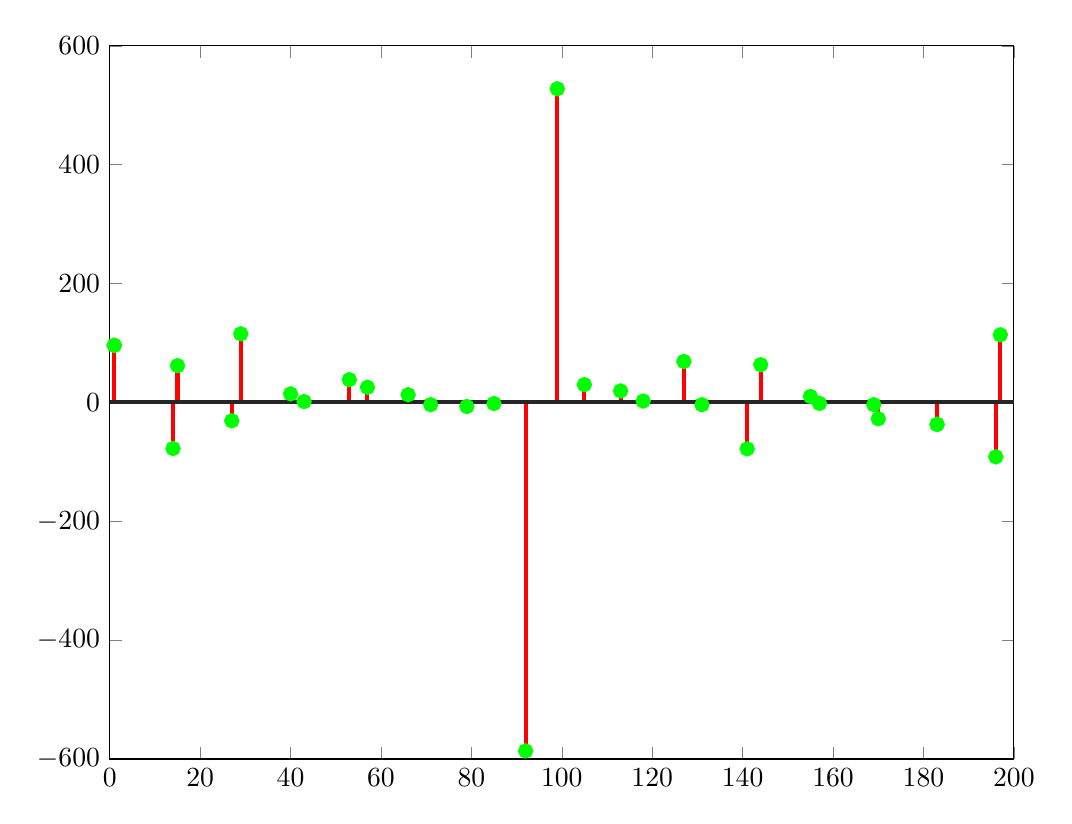
\begin{tikzpicture}

\begin{axis}[%
width=4.521in,
height=3.566in,
at={(0.758in,0.481in)},
scale only axis,
xmin=0,
xmax=200,
ymin=-600,
ymax=600,
axis background/.style={fill=white}
]
\addplot[ycomb, color=red, line width=1.5pt, mark=*, mark options={solid, fill=red, green}, forget plot] table[row sep=crcr] {%
1	96\\
15	61.8405159676837\\
29	115.396461869287\\
43	1.39320614430019\\
57	25.4543162795665\\
71	-3.824409687939\\
85	-1.90254204745981\\
99	527.693372169007\\
113	19.3349778052062\\
127	68.938951416754\\
141	-78.1377674149945\\
155	9.99707529364864\\
169	-3.75059930092979\\
183	-36.9748518197181\\
197	113.813269618881\\
1	96\\
14	-77.5471454188034\\
27	-30.9232662713007\\
40	14.3497108293358\\
53	38.2537557025721\\
66	12.8778537782972\\
79	-6.8710448873182\\
92	-586.390764014078\\
105	29.9833721024771\\
118	2.33185767595022\\
131	-3.824409687939\\
144	63.507357731341\\
157	-1.71860486624029\\
170	-27.5315139371526\\
183	-36.9748518197181\\
196	-91.5921246182205\\
};
\addplot[forget plot, color=white!15!black, line width=1.5pt] table[row sep=crcr] 
	%%\end{figure}
	%%\end{column}
	%
	%\end{columns}
\end{frame}
%-----------------------------------------
\begin{frame}\frametitle{Sparse Fourier Transform Approach}
	 	\begin{itemize}
	 		\item {\color{blue} \cite{pawar2014robust}}: Robust Sparse Fourier Transform
	 		\begin{itemize}
	 			\item[-] Sparse graph code approach
	 			\item[-] Computational complexity : $O(N \log N)$
	 		\end{itemize}
	 		
	 		\item {\color{blue} \cite{hassanieh2012faster}}: Faster GPS receiver
	 		\begin{itemize}
	 			\item[-] Exploited sparsity in Correlation function $R_{XY}$
	 		\end{itemize}
	 		
	 	\end{itemize}	 	

\end{frame}
%---------------------------------------------------------
\begin{frame}\frametitle{Sparse Fourier Transform Approach}
	\begin{figure}[t]
		\centering
		\scalebox{0.28}{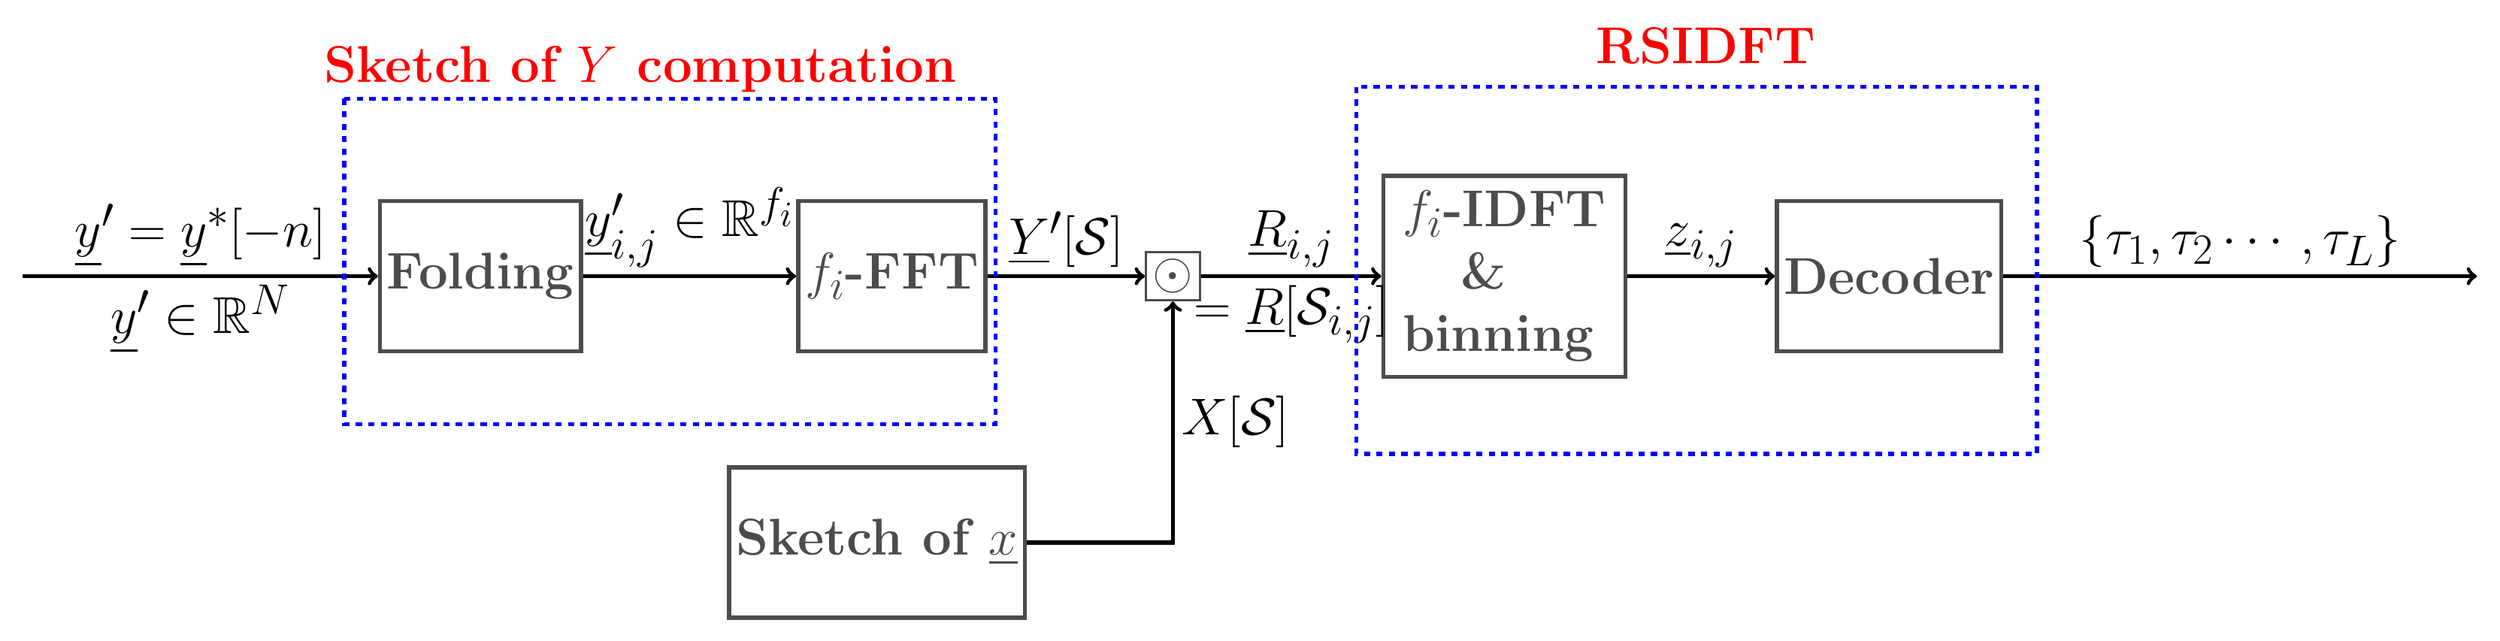
\begin{tikzpicture}

\def\nodewidth{1in}
\def\fsize{\Huge}
\tikzstyle{block} = [rectangle, draw, thick,opacity=0.7,line width =2, minimum size=\nodewidth]
\tikzstyle{opnode} = [rectangle, draw, thick,opacity=0.7,line width=1, minimum size=0.2in]

\node[block] (r1) at (-8.7,3){\fsize \bf Folding};
\node[block] (r2) at (-1.75,3) {\fsize \bf $f_i$-FFT};
\node[opnode] (r3) at (3,3) {\fsize \bf $\odot$};
\node[block,align=center] (r4) at (8.6,3) {\fsize \bf \begin{tabular}{l}
$f_i$-IDFT \\ 
~~ \& \\ 
binning
\end{tabular}};
\node[block] (r5) at (15.1,3) {\fsize \bf Decoder};
\node[block] (r6) at (-2,-1.5) {\fsize \bf Sketch of $\xv$};


\draw[<-, thick, line width=2] (r1.west)--node[midway, above]{\fsize $\yv'=\yv^*[-n]$}
node[midway, below]{\fsize $\yv'\in\mathbb{R}^N$}+(-6,0);
\draw[->, thick, line width=2] (r1.east)--node[midway, above]{\fsize $\yv'_{i,j}\in\mathbb{R}^{f_i}$}(r2.west);
\draw[->, thick, line width=2] (r2.east)--node[midway, above]{\fsize $\Yv'[\mc{S}]$}(r3.west);
\draw[->, thick, line width=2] (r3.east)--node[midway, above]{\fsize $\Rv_{i,j}$}
node[midway,below]{\fsize \bf $=\Rv[\mathcal{S}_{i,j}]$}(r4.west);
\draw[->, thick, line width=2] (r4.east)--node[midway, above]{\fsize $\zv_{i,j}$}(r5.west);
\draw[->, thick, line width=2] (r5.east)--node[midway, above]{\fsize $\{\tau_1, \tau_2 \cdots, \tau_L \}$}+(8,0);
\draw[->, thick, line width=2] let \p1=(r6),\p2= (r3) in (r6.east)--(\x2,\y1)--node[midway, right]{\fsize \bf $X[\mathcal{S}]$}  (r3.south);



\draw [dashed, line width =2, color=blue] (-11,6) rectangle (0,0.5);
\node[color= red] at (-6,6.5) {\fsize \bf  Sketch of $Y$ computation};
\draw [dashed, line width =2, color=blue]  (6.1,6.2) rectangle (17.6,0);
\node [color = red] at (12,6.9) {\fsize \bf RSIDFT};
\end{tikzpicture}}
	\end{figure}
\vspace{-0.2cm}
	 	\begin{block}{}
	 		\begin{equation}\label{eqn:Rxy_fourier}\nonumber
	 		\boxed{\rv = \underset{\text{\color{red} 3 } } {\mathcal{F}_{N}^{-1}} \ \{ \underset{\text{ \color{red} 1 } }{  \mathcal{F}_{N}\{\xv\}}  \odot \ \underset{\text{ \color{red} 2 } }{ \mathcal{F}_{N}\{\yv'\}}  \} }
	 		\end{equation}
	 		
	 		\begin{itemize}
	 			\item[\color{red} 1.] \textit{\color{blue} Sketch of $\xv$ : }  Assume $ \Xv[l] = \mathcal{F}\{\xv\}$ is precomputed at positions $l \in \mathcal{S}$.
	 			
	 			\item[\color{red} 2.] \textit{\color{blue} Sketch of $\yv$:}  Compute $ \Yv'[l] = \mathcal{F}\{\yv'\}$ for $l \in \mathcal{S}$.
	 			\begin{itemize}
	 				\item[-] Only $M$ non-zero values in $\yv'$ - Efficient computation (folding and adding)
	 			\end{itemize}
	 			
	 			\item[\color{red} 3.] \textit{\color{blue} Sparse $\mathcal{F}^{-1}$}:
	 			\begin{itemize}
	 				\item[-] Robust Sparse Inverse Fourier Transform (RSIDFT)
	 				\item[-] Efficient Implementation- {\color{blue} sublinear} time and sampling complexity
	 			\end{itemize}
	 		\end{itemize}
	 	\end{block}
\end{frame}


%------------------------------------------------------------------
\begin{frame}{Robust Sparse Inverse Fourier Transform(RSIDFT)}
\begin{block}{Main Idea}
	\begin{itemize}
		\item \alert{Sub-sampling} in frequency corresponds to \alert{aliasing} in time
		\item Aliased coefficients $\Leftrightarrow$ parity check constraints of \alert{GLDPC codes}
		\item \alert{CRT} guided sub-sampling induces a code good for \alert{Peeling decoder}
		\item R-FFAST- proposed by Pawar and Ramchandran 2014
	\end{itemize}
\end{block}
\begin{block}{Key modifications}
   \begin{itemize}
   	\item Optimized for the induced noise model
   	\item Correlation peak is always {\color{blue} positive}
   	\item Take advantage in decoding algorithm - {\color{blue}sub-linear} time complexity
   \end{itemize}
\end{block}
\end{frame}

%--------------------------------------------------------------------------------------
	\begin{frame}{Aliasing and Sparse Graph Codes}
		
\only<1>{  \begin{block}{IDFT Computation($N=6$)}
			\begin{figure}[t]
				\centering
				\includegraphics[width=3.1in]{X_DFT}
			\end{figure}
		\end{block}
		
		\begin{columns}
			
			\column{.47\textwidth}
			\begin{block}{{\small $\color{red}x_s$:\ Sub-sampled by $P_1=2$}}
				\begin{figure}[t]
					\centering
					\includegraphics[width=2.3in]{Xs}
				\end{figure}
			\end{block}
			
			\begin{block}{{\small$\color{red}z_s$:\ Sub-sampled by $P_2=3$}}
				\begin{figure}[t]
					\centering
					\includegraphics[width=2.3in]{Zs}
				\end{figure}
			\end{block}
			
			\column{.47\textwidth}
			\begin{block}{\small Factor graph}
				\begin{figure}[t]
					\centering
					\includegraphics[width=2.3in]{Factorgraph_example}
				\end{figure}
			\end{block}
		\end{columns}}

\only<2>{ \begin{block}{IDFT Computation($N=6$)}
		\begin{figure}[t]
			\centering
			\includegraphics[width=3.1in]{X_DFT}
		\end{figure}
	\end{block}
	
	\begin{columns}
		
		\column{.47\textwidth}
		\begin{block}{{\small $\color{red}\tilde{x}_s$:\ Sub-sampled by $P_1=2$ ({\color{blue}shifted})}}
			\begin{figure}[t]
				\centering
				\includegraphics[width=2.3in]{Xs_shift}
			\end{figure}
		\end{block}
		
		\begin{block}{{\small$\color{red}\tilde{z}_s$:\ Sub-sampled by $P_2=3$ ({\color{blue}shifted})}}
			\begin{figure}[t]
				\centering
				\includegraphics[width=2.3in]{Zs_shift}
			\end{figure}
		\end{block}
		
		\column{.47\textwidth}
		\begin{block}{\small Factor graph}
			\begin{figure}[t]
				\centering
				\includegraphics[width=2.3in]{Factorgraph_example_tilde}
			\end{figure}
		\end{block}
	\end{columns}}
		
	\end{frame}

\begin{frame}\frametitle{RSIDFT Framework}
	
		\begin{figure}[t!]
			\begin{center}
				\resizebox{0.8\textwidth}{!}{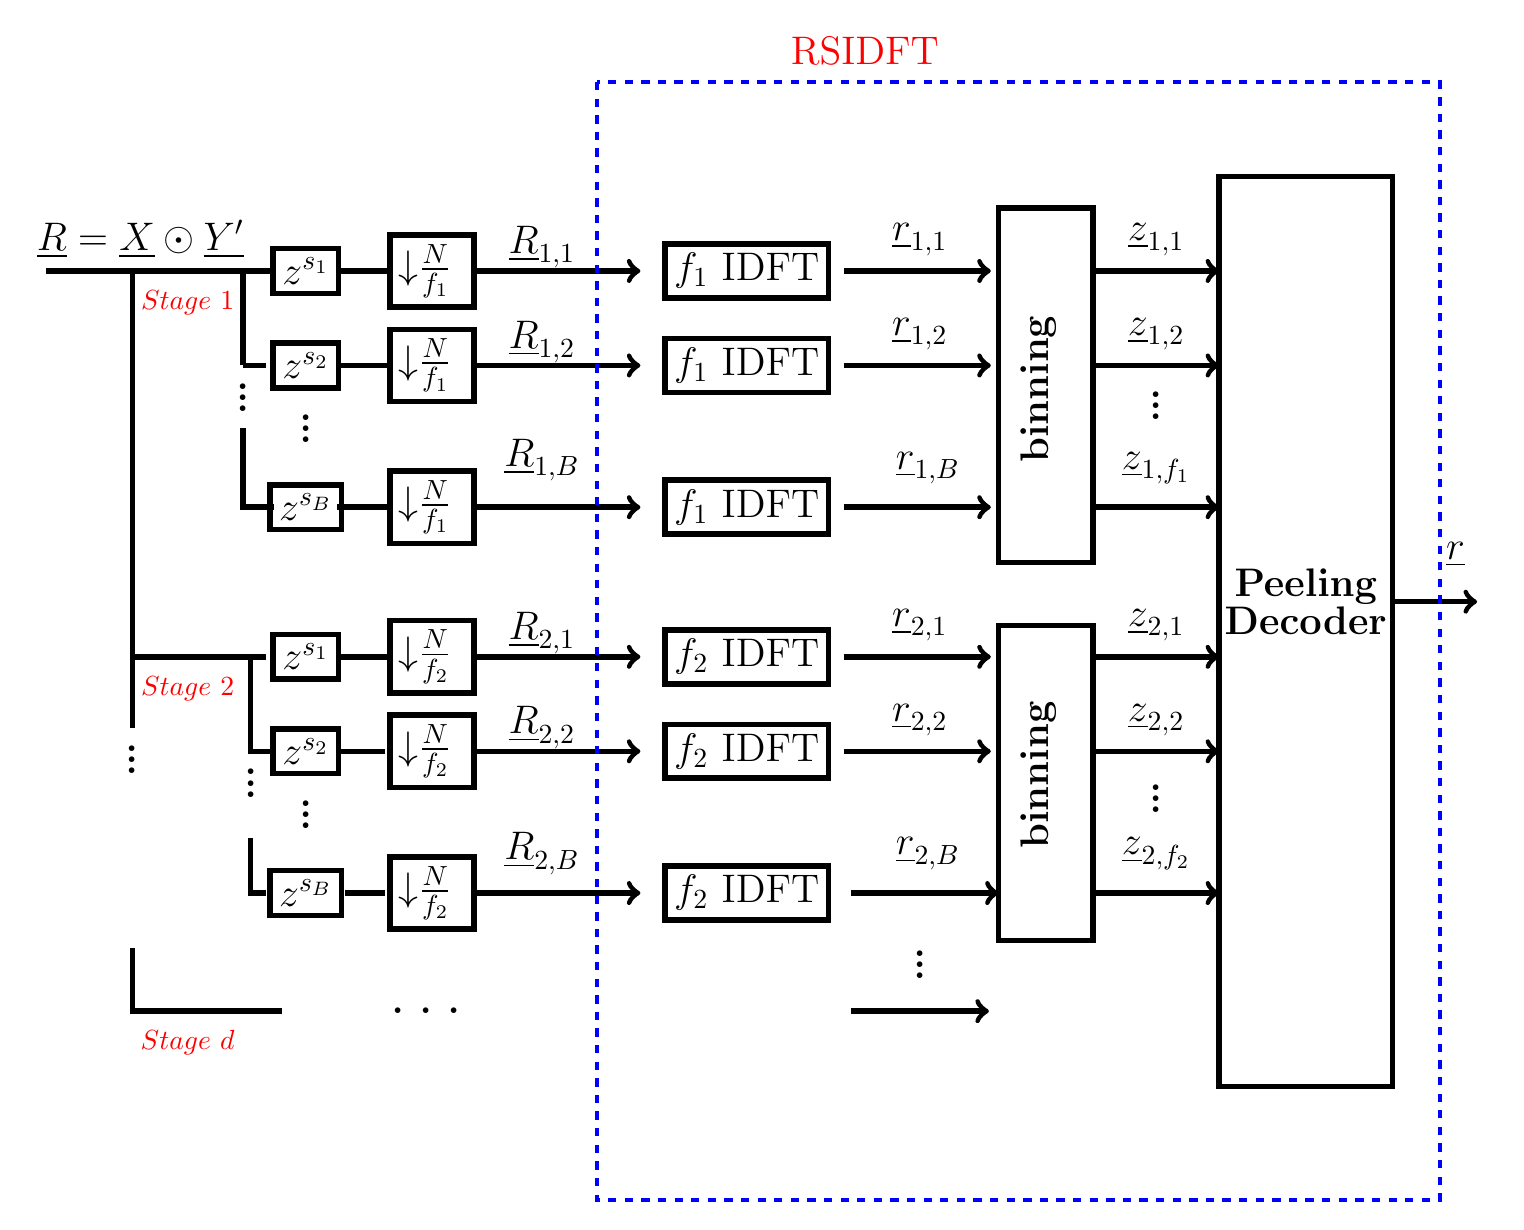
\begin{tikzpicture}

 % Downsampling blocks
\node[draw,align=center,thick,line  width =2pt] at (1.8,4.5) {\Large{$\mathbf{\downarrow} \frac{N}{f_2}$} };
\node[draw,align=center,thick,line  width =2pt] at (1.8,5.7) {\Large{$\mathbf{\downarrow} \frac{N}{f_2}$ }};
\node[draw,align=center,thick,line  width =2pt] (v6) at (1.8,2.7) {\Large{$\mathbf{\downarrow} \frac{N}{f_2}$ }};

\node[draw,align=center,thick,line  width =2pt] at (1.8,9.4) {\Large{$\mathbf{\downarrow} \frac{N}{f_1}$} };
\node[draw,align=center,thick,line  width =2pt] at (1.8,10.6) {\Large{$\mathbf{\downarrow} \frac{N}{f_1}$ }};
\node[draw,align=center,thick,line  width =2pt] at (1.8,7.6) {\Large{$\mathbf{\downarrow} \frac{N}{f_1}$ }};

%  Input lines to the down-sampling block

%  Delay blocks
\node[draw,align=center,thick,line  width =2pt] at (0.2,10.6) {\bf \Large{$z^{s_1}$}};
\node[draw,align=center,thick,line  width =2pt] at (0.2,9.4) {\bf \Large{$z^{s_2}$}};
\node[draw,align=center,thick,line  width =2pt] at (0.2,7.6) {\bf \Large{$z^{s_B}$}};

\node[draw,align=center,thick,line  width =2pt] at (0.2,5.7) {\bf \Large{$z^{s_1}$}};
\node[draw,align=center,thick,line  width =2pt] at (0.2,4.5) {\bf \Large{$z^{s_2}$}};
\node[draw,align=center,thick,line  width =2pt] at (0.2,2.7) {\bf \Large{$z^{s_B}$}};


% paths connecting the delay blocks  
 
 \draw[thick,line  width =2pt] (1.3,9.4) -- (0.6,9.4);
 

\node[line  width =2pt] at (-0.6,9.1) {\Huge{\vdots}};
\node[line  width =2pt] at (0.2,8.7) {\Huge{\vdots}};
\node[line  width =2pt] at (-0.5,4.2) {\Huge{\vdots}};
\node[line  width =2pt] at (0.2,3.8) {\Huge{\vdots}};

 \draw[thick,line  width =2pt] (1.3,10.6) -- (0.6,10.6);
 \draw[thick,line  width =2pt] (-0.6,9.4) -- (-0.6,10.6);
 
% paths connecting the two stages   
 \draw[thick,line  width =2pt] (-0.2,10.6) -- (-2,10.6);
 \draw[thick,line  width =2pt] (-0.6,9.4) -- (-0.3,9.4);
 \draw[thick,line  width =2pt] (-0.3,5.7) -- (-2,5.7);
 \draw[thick,line  width =2pt] (-2,5.7) -- (-2,10.6);
  \draw[thick,line  width =2pt] (-3.1,10.6) -- (-2,10.6);
  \draw[thick,line  width =2pt] (-2,5.7) -- (-2,4.8);
  
  
  % DFT blocks
\node[draw,align=center,thick,line  width =2pt] at (5.8,4.5) {\Large{$f_2$ IDFT}};
\node[draw,align=center,thick,line  width =2pt] at (5.8,5.7) {\Large{$f_2$ IDFT}};
\node[draw,align=center,thick,line  width =2pt] at (5.8,2.7) {\Large{$f_2$ IDFT}};

\node[draw,align=center,thick,line  width =2pt] at (5.8,9.4) {\Large{$f_1$ IDFT}};
\node[draw,align=center,thick,line  width =2pt] at (5.8,10.6) {\Large{$f_1$ IDFT}};
\node[draw,align=center,thick,line  width =2pt] at (5.8,7.6) {\Large{$f_1$ IDFT}};
% Connectors
 \draw[->,thick,line  width =2pt] (2.35,10.6) -- (4.45,10.6);
 \draw[->,thick,line  width =2pt] (2.35,9.4) -- (4.45,9.4);
 \draw[->,thick,line  width =2pt] (2.35,7.6) -- (4.45,7.6);
 
 \draw[->,thick,line  width =2pt] (2.35,5.7) -- (4.45,5.7);
 \draw[->,thick,line  width =2pt] (2.35,4.5) -- (4.45,4.5);
 \draw[->,thick,line  width =2pt] (2.35,2.7) -- (4.45,2.7);

 \draw[->,thick,line  width =2pt] (10.23,10.6) -- (11.8,10.6);
 \draw[->,thick,line  width =2pt] (10.23,9.4) -- (11.8,9.4);
 \draw[->,thick,line  width =2pt] (10.23,7.6) -- (11.8,7.6);
 
 \draw[->,thick,line  width =2pt] (10.23,5.7) -- (11.8,5.7);
 \draw[->,thick,line  width =2pt] (10.23,4.5) -- (11.8,4.5);
 \draw[->,thick,line  width =2pt] (10.23,2.7) -- (11.8,2.7);
 
  \draw[->,thick,line  width =2pt] (7.03,10.6) -- (8.9,10.6);
 \draw[->,thick,line  width =2pt] (7.03,9.4) -- (8.9,9.4);
 \draw[->,thick,line  width =2pt] (7.03,7.6) -- (8.9,7.6);
 
 \draw[->,thick,line  width =2pt] (7.03,5.7) -- (8.9,5.7);
 \draw[->,thick,line  width =2pt] (7.03,4.5) -- (8.9,4.5);
 \draw[->,thick,line  width =2pt] (7.13,2.7) -- (9,2.7);
 
  % Labels
  \node[draw=none,align=center] at (-1.9,11) {\Large{$\Rv= \underline{X} \odot \underline{Y'}$}};
  
  \node[draw=none,align=center] at (3.2,10.9) {\Large{$\Rv_{1,1}$}};
  \node[draw=none,align=center] at (3.2,9.7) {\Large{$\Rv_{1,2}$}};
\node[draw=none,align=center] at (3.2,8.2) {\Large{$\Rv_{1,B}$}};

\node[draw=none,align=center] at (3.2,6) {\Large{$\Rv_{2,1}$}};
  \node[draw=none,align=center] at (3.2,4.8) {\Large{$\Rv_{2,2}$}};
  \node[draw=none,align=center] at (3.2,3.2) {\Large{$\Rv_{2,B}$}};

  \node[draw=none,align=center] at (8,11) {\Large{$\rv_{1,1}$}};
  \node[draw=none,align=center] at (8,9.8) {\Large{$\rv_{1,2}$}};
  \node[draw=none,align=center] at (8.1,8.1) {\Large{$\rv_{1,B}$}};
  
    \node[draw=none,align=center] at (11,11) {\Large{$\zv_{1,1}$}};
  \node[draw=none,align=center] at (11,9.8) {\Large{$\zv_{1,2}$}};
  \node[draw=none,align=center] at (11,8.1) {\Large{$\zv_{1,f_1}$}};
  
     \node [draw=none] at (11,9) {\Huge{\vdots}} ;
   
  \node[draw=none,align=center] at (8,6.1) {\Large{$\rv_{2,1}$}};
  \node[draw=none,align=center] at (8,4.9) {\Large{$\rv_{2,2}$}};
  \node[draw=none,align=center] at (8.1,3.2) {\Large{$\rv_{2,B}$}};
  
  \node [draw=none] at (11,4) {\Huge{\vdots}} ;
  
    \node[draw=none,align=center] at (11,6.1) {\Large{$\zv_{2,1}$}};
  \node[draw=none,align=center] at (11,4.9) {\Large{$\zv_{2,2}$}};
  \node[draw=none,align=center] at (11,3.2) {\Large{$\zv_{2,f_2}$}};
  
  \node [draw=none] at (-2,4.5) {\Huge{\vdots}} ;
  
   \node[draw=none,align=center] at (-1.3,10.2) {\color{red}$Stage ~1$};
  \node[draw=none,align=center] at (-1.3,5.3) {\color{red}$Stage ~2$};
   \node[draw=none,align=center] at (-1.3,0.8) {\color{red}$Stage ~d$};
\draw [thick,line  width =2pt](-2,2) -- (-2,1.2) -- (-0.1,1.2) ;
 \node[draw=none,align=center] at (1.8,1.2) {\Huge{\ldots}};
 
\draw [thick,line  width =2pt] (11.8,0.2424) rectangle (14,11.8);
\node (v1) at (7,1.2) {};
\node (v2) at (9,1.2) {};



\node (v11) at (1.3,7.6) {};


\draw  [->,thick,line  width =2pt](v1) edge (v2);
\node at (8,1.9) {\Huge{\vdots}};
\node [text width=3cm, align =center ] at (12.9,6.4) {\Large \bf Peeling \\ Decoder};
\node (v3) at (13.9,6.4) {};
\node (v4) at (15.2,6.4) {};
\draw [thick, ->,line  width =2pt] (v3) edge (v4);
\node at (14.8,7) {\Large{$\rv$}};

\draw[thick,line  width =2pt] (-0.6,8.6) -- (-0.6,7.6) -- (-0.2,7.6);
\draw[thick,line  width =2pt] (0.6,7.6) -- (1.3,7.6);
\draw[thick,line  width =2pt] (-0.5,5.7) -- (-0.5,4.5) -- (-0.2,4.5);
\draw[thick,line  width =2pt] (-0.5,3.4) -- (-0.5,2.7) -- (-0.3,2.7);
\draw [thick,line  width =2pt](0.6,5.7) -- (1.3,5.7);
\draw[thick,line  width =2pt] (0.6,4.5) -- (1.2,4.5);
\draw[thick,line  width =2pt] (0.7,2.7) -- (1.2,2.7);
\draw [dashed, color=blue, line width =1.5pt ] (3.9,13) rectangle (14.6,-1.2);
\node[color =red] at (7.3,13.4) {\Large RSIDFT  };
\draw [thick, line width =2pt]  (9,11.4) rectangle (10.2,6.9);
\draw [thick, line width =2pt]  (9,6.1) rectangle (10.2,2.1);
\node[rotate=90] at (9.5,9.1) {\Large \bf binning};
\node[rotate=90] at (9.5,4.2) {\Large \bf binning};
\end{tikzpicture}}
				%	 		\includegraphics[height=7cm]{Figures/FFAST_Robust}
			\end{center}	
			\label{fig:rsidft}
			\vspace{5 pt}
		\end{figure}
\end{frame}


\begin{frame}\frametitle{RSIDFT Framework}
	\begin{columns}
		\column[]{0.43\columnwidth}
\begin{figure}[t!]
	\begin{center}
		\resizebox{1.05\textwidth}{0.7\textheight}{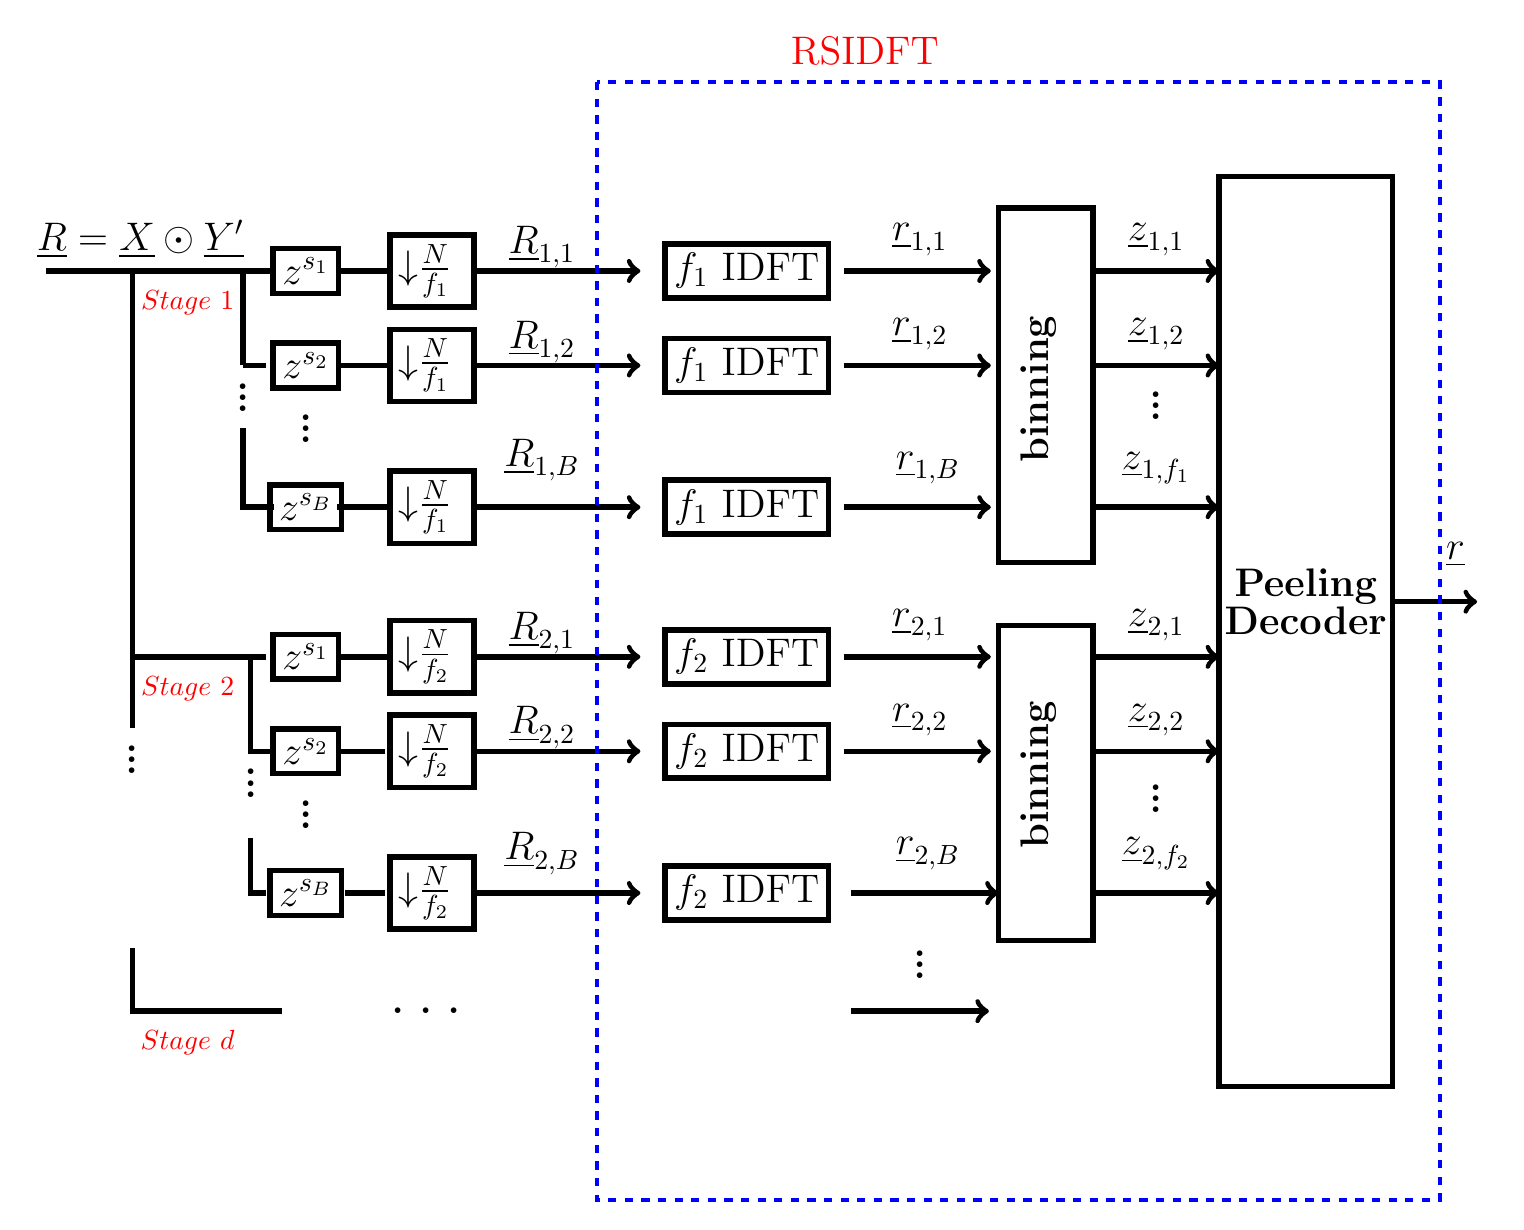
\begin{tikzpicture}

 % Downsampling blocks
\node[draw,align=center,thick,line  width =2pt] at (1.8,4.5) {\Large{$\mathbf{\downarrow} \frac{N}{f_2}$} };
\node[draw,align=center,thick,line  width =2pt] at (1.8,5.7) {\Large{$\mathbf{\downarrow} \frac{N}{f_2}$ }};
\node[draw,align=center,thick,line  width =2pt] (v6) at (1.8,2.7) {\Large{$\mathbf{\downarrow} \frac{N}{f_2}$ }};

\node[draw,align=center,thick,line  width =2pt] at (1.8,9.4) {\Large{$\mathbf{\downarrow} \frac{N}{f_1}$} };
\node[draw,align=center,thick,line  width =2pt] at (1.8,10.6) {\Large{$\mathbf{\downarrow} \frac{N}{f_1}$ }};
\node[draw,align=center,thick,line  width =2pt] at (1.8,7.6) {\Large{$\mathbf{\downarrow} \frac{N}{f_1}$ }};

%  Input lines to the down-sampling block

%  Delay blocks
\node[draw,align=center,thick,line  width =2pt] at (0.2,10.6) {\bf \Large{$z^{s_1}$}};
\node[draw,align=center,thick,line  width =2pt] at (0.2,9.4) {\bf \Large{$z^{s_2}$}};
\node[draw,align=center,thick,line  width =2pt] at (0.2,7.6) {\bf \Large{$z^{s_B}$}};

\node[draw,align=center,thick,line  width =2pt] at (0.2,5.7) {\bf \Large{$z^{s_1}$}};
\node[draw,align=center,thick,line  width =2pt] at (0.2,4.5) {\bf \Large{$z^{s_2}$}};
\node[draw,align=center,thick,line  width =2pt] at (0.2,2.7) {\bf \Large{$z^{s_B}$}};


% paths connecting the delay blocks  
 
 \draw[thick,line  width =2pt] (1.3,9.4) -- (0.6,9.4);
 

\node[line  width =2pt] at (-0.6,9.1) {\Huge{\vdots}};
\node[line  width =2pt] at (0.2,8.7) {\Huge{\vdots}};
\node[line  width =2pt] at (-0.5,4.2) {\Huge{\vdots}};
\node[line  width =2pt] at (0.2,3.8) {\Huge{\vdots}};

 \draw[thick,line  width =2pt] (1.3,10.6) -- (0.6,10.6);
 \draw[thick,line  width =2pt] (-0.6,9.4) -- (-0.6,10.6);
 
% paths connecting the two stages   
 \draw[thick,line  width =2pt] (-0.2,10.6) -- (-2,10.6);
 \draw[thick,line  width =2pt] (-0.6,9.4) -- (-0.3,9.4);
 \draw[thick,line  width =2pt] (-0.3,5.7) -- (-2,5.7);
 \draw[thick,line  width =2pt] (-2,5.7) -- (-2,10.6);
  \draw[thick,line  width =2pt] (-3.1,10.6) -- (-2,10.6);
  \draw[thick,line  width =2pt] (-2,5.7) -- (-2,4.8);
  
  
  % DFT blocks
\node[draw,align=center,thick,line  width =2pt] at (5.8,4.5) {\Large{$f_2$ IDFT}};
\node[draw,align=center,thick,line  width =2pt] at (5.8,5.7) {\Large{$f_2$ IDFT}};
\node[draw,align=center,thick,line  width =2pt] at (5.8,2.7) {\Large{$f_2$ IDFT}};

\node[draw,align=center,thick,line  width =2pt] at (5.8,9.4) {\Large{$f_1$ IDFT}};
\node[draw,align=center,thick,line  width =2pt] at (5.8,10.6) {\Large{$f_1$ IDFT}};
\node[draw,align=center,thick,line  width =2pt] at (5.8,7.6) {\Large{$f_1$ IDFT}};
% Connectors
 \draw[->,thick,line  width =2pt] (2.35,10.6) -- (4.45,10.6);
 \draw[->,thick,line  width =2pt] (2.35,9.4) -- (4.45,9.4);
 \draw[->,thick,line  width =2pt] (2.35,7.6) -- (4.45,7.6);
 
 \draw[->,thick,line  width =2pt] (2.35,5.7) -- (4.45,5.7);
 \draw[->,thick,line  width =2pt] (2.35,4.5) -- (4.45,4.5);
 \draw[->,thick,line  width =2pt] (2.35,2.7) -- (4.45,2.7);

 \draw[->,thick,line  width =2pt] (10.23,10.6) -- (11.8,10.6);
 \draw[->,thick,line  width =2pt] (10.23,9.4) -- (11.8,9.4);
 \draw[->,thick,line  width =2pt] (10.23,7.6) -- (11.8,7.6);
 
 \draw[->,thick,line  width =2pt] (10.23,5.7) -- (11.8,5.7);
 \draw[->,thick,line  width =2pt] (10.23,4.5) -- (11.8,4.5);
 \draw[->,thick,line  width =2pt] (10.23,2.7) -- (11.8,2.7);
 
  \draw[->,thick,line  width =2pt] (7.03,10.6) -- (8.9,10.6);
 \draw[->,thick,line  width =2pt] (7.03,9.4) -- (8.9,9.4);
 \draw[->,thick,line  width =2pt] (7.03,7.6) -- (8.9,7.6);
 
 \draw[->,thick,line  width =2pt] (7.03,5.7) -- (8.9,5.7);
 \draw[->,thick,line  width =2pt] (7.03,4.5) -- (8.9,4.5);
 \draw[->,thick,line  width =2pt] (7.13,2.7) -- (9,2.7);
 
  % Labels
  \node[draw=none,align=center] at (-1.9,11) {\Large{$\Rv= \underline{X} \odot \underline{Y'}$}};
  
  \node[draw=none,align=center] at (3.2,10.9) {\Large{$\Rv_{1,1}$}};
  \node[draw=none,align=center] at (3.2,9.7) {\Large{$\Rv_{1,2}$}};
\node[draw=none,align=center] at (3.2,8.2) {\Large{$\Rv_{1,B}$}};

\node[draw=none,align=center] at (3.2,6) {\Large{$\Rv_{2,1}$}};
  \node[draw=none,align=center] at (3.2,4.8) {\Large{$\Rv_{2,2}$}};
  \node[draw=none,align=center] at (3.2,3.2) {\Large{$\Rv_{2,B}$}};

  \node[draw=none,align=center] at (8,11) {\Large{$\rv_{1,1}$}};
  \node[draw=none,align=center] at (8,9.8) {\Large{$\rv_{1,2}$}};
  \node[draw=none,align=center] at (8.1,8.1) {\Large{$\rv_{1,B}$}};
  
    \node[draw=none,align=center] at (11,11) {\Large{$\zv_{1,1}$}};
  \node[draw=none,align=center] at (11,9.8) {\Large{$\zv_{1,2}$}};
  \node[draw=none,align=center] at (11,8.1) {\Large{$\zv_{1,f_1}$}};
  
     \node [draw=none] at (11,9) {\Huge{\vdots}} ;
   
  \node[draw=none,align=center] at (8,6.1) {\Large{$\rv_{2,1}$}};
  \node[draw=none,align=center] at (8,4.9) {\Large{$\rv_{2,2}$}};
  \node[draw=none,align=center] at (8.1,3.2) {\Large{$\rv_{2,B}$}};
  
  \node [draw=none] at (11,4) {\Huge{\vdots}} ;
  
    \node[draw=none,align=center] at (11,6.1) {\Large{$\zv_{2,1}$}};
  \node[draw=none,align=center] at (11,4.9) {\Large{$\zv_{2,2}$}};
  \node[draw=none,align=center] at (11,3.2) {\Large{$\zv_{2,f_2}$}};
  
  \node [draw=none] at (-2,4.5) {\Huge{\vdots}} ;
  
   \node[draw=none,align=center] at (-1.3,10.2) {\color{red}$Stage ~1$};
  \node[draw=none,align=center] at (-1.3,5.3) {\color{red}$Stage ~2$};
   \node[draw=none,align=center] at (-1.3,0.8) {\color{red}$Stage ~d$};
\draw [thick,line  width =2pt](-2,2) -- (-2,1.2) -- (-0.1,1.2) ;
 \node[draw=none,align=center] at (1.8,1.2) {\Huge{\ldots}};
 
\draw [thick,line  width =2pt] (11.8,0.2424) rectangle (14,11.8);
\node (v1) at (7,1.2) {};
\node (v2) at (9,1.2) {};



\node (v11) at (1.3,7.6) {};


\draw  [->,thick,line  width =2pt](v1) edge (v2);
\node at (8,1.9) {\Huge{\vdots}};
\node [text width=3cm, align =center ] at (12.9,6.4) {\Large \bf Peeling \\ Decoder};
\node (v3) at (13.9,6.4) {};
\node (v4) at (15.2,6.4) {};
\draw [thick, ->,line  width =2pt] (v3) edge (v4);
\node at (14.8,7) {\Large{$\rv$}};

\draw[thick,line  width =2pt] (-0.6,8.6) -- (-0.6,7.6) -- (-0.2,7.6);
\draw[thick,line  width =2pt] (0.6,7.6) -- (1.3,7.6);
\draw[thick,line  width =2pt] (-0.5,5.7) -- (-0.5,4.5) -- (-0.2,4.5);
\draw[thick,line  width =2pt] (-0.5,3.4) -- (-0.5,2.7) -- (-0.3,2.7);
\draw [thick,line  width =2pt](0.6,5.7) -- (1.3,5.7);
\draw[thick,line  width =2pt] (0.6,4.5) -- (1.2,4.5);
\draw[thick,line  width =2pt] (0.7,2.7) -- (1.2,2.7);
\draw [dashed, color=blue, line width =1.5pt ] (3.9,13) rectangle (14.6,-1.2);
\node[color =red] at (7.3,13.4) {\Large RSIDFT  };
\draw [thick, line width =2pt]  (9,11.4) rectangle (10.2,6.9);
\draw [thick, line width =2pt]  (9,6.1) rectangle (10.2,2.1);
\node[rotate=90] at (9.5,9.1) {\Large \bf binning};
\node[rotate=90] at (9.5,4.2) {\Large \bf binning};
\end{tikzpicture}}
		%	 		\includegraphics[height=7cm]{Figures/FFAST_Robust}
		\end{center}	
		\label{fig:rsidft}
		\vspace{5 pt}
		\end{figure}
		\column[]{0.53\columnwidth}
		\begin{figure}[h!]
			\begin{center}
				%		\includegraphics[height=7cm]{Figures/Factorgraph}
				\resizebox{1.0\textwidth}{0.65\textheight}{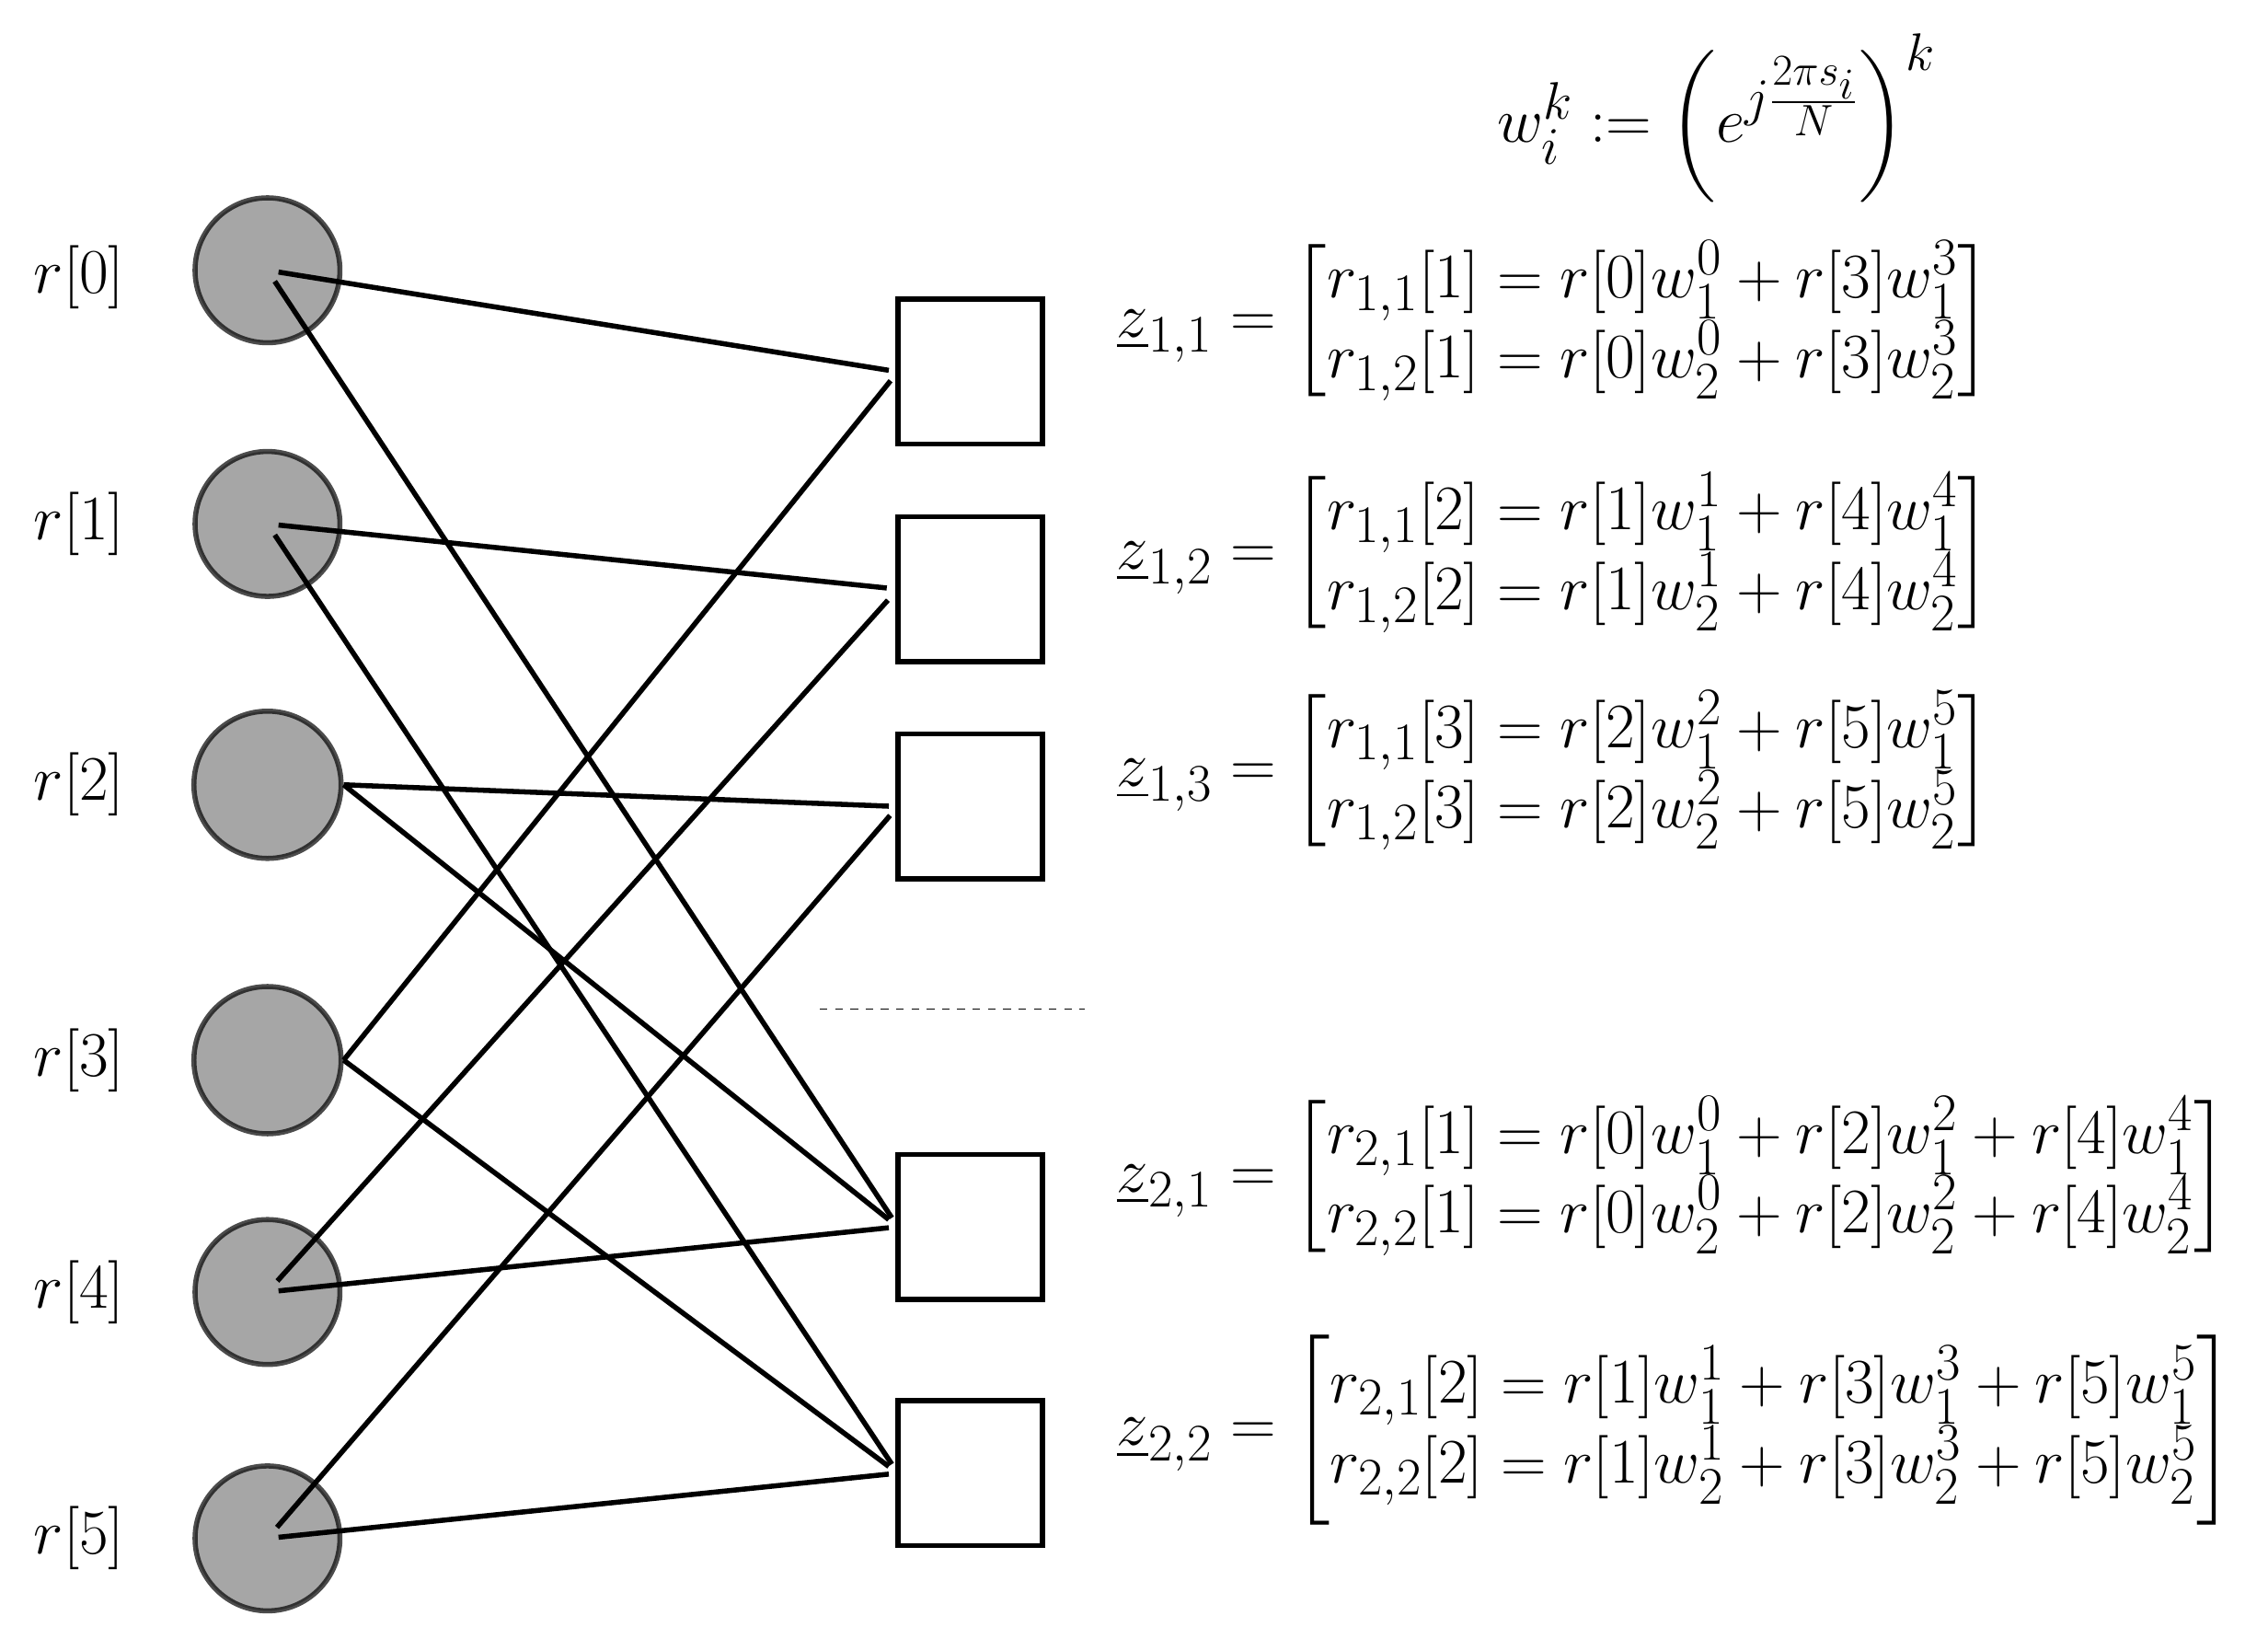
\begin{tikzpicture}

\definecolor{brightturquoise}{rgb}{0.03, 0.91, 0.87}
\definecolor{buff}{rgb}{0.94, 0.86, 0.51}
\definecolor{caribbeangreen}{rgb}{0.0, 0.8, 0.6}
\definecolor{celadon}{rgb}{0.67, 0.88, 0.69}
\definecolor{darktangerine}{rgb}{1.0, 0.66, 0.07}
\definecolor{darkviolet}{rgb}{0.58, 0.0, 0.83}
\definecolor{deepskyblue}{rgb}{0.0, 0.75, 1.0}
\definecolor{amber(sae/ece)}{rgb}{1.0, 0.49, 0.0}
\definecolor{antiquewhite}{rgb}{0.98, 0.92, 0.84}
\definecolor{applegreen}{rgb}{0.55, 0.71, 0.0}
\definecolor{babyblue}{rgb}{0.54, 0.81, 0.94}

\def\nodewidth{0.8in}
\tikzstyle{bit} = [circle, draw, thick,fill=gray,opacity=0.7,line width =2, minimum size=\nodewidth]

% Variable nodes 
\node[bit] (v6) at (-7,-6){};
\node[bit] (v5) at (-7,-2.2) {};
%\draw[thick,fill=gray,line width =2,opacity=0.7]  (-7,-2.2) node (v5) {} ellipse (1 and 1);
\draw [thick,fill=gray,line width =2,opacity=0.7]  (-7,1.4) node (v3) {} ellipse (1 and 1);
\draw  [thick,fill=gray,line width =2,opacity=0.7]  (-7,-9.2) node (v1) {} ellipse (1 and 1);
\draw  [thick,fill=gray,line width =2,opacity=0.7]  (-7,-12.6) node (v1_1) {} ellipse (1 and 1);
\draw  [thick,fill=gray,line width =2,opacity=0.7]  (-7,4.9) node (v1_2) {} ellipse (1 and 1);

%Check nodes
\draw [thick,line width =2] (1.7,4.5) rectangle (3.7,2.5);
\draw [thick,line width =2]  (1.7,1.5) node (v8) {} rectangle (3.7,-0.5);
\draw [thick,line width =2] (1.7,-1.5) rectangle (3.7,-3.5);
\draw [thick,line width =2] (1.7,-7.3) rectangle (3.7,-9.3);
\draw [thick,line width =2] (1.7,-10.7) rectangle (3.7,-12.7);

\node (v2) at (1.7,3.5) {};
\node (v4) at (1.7,-2.5) {};
\node (v7) at (1.7,-8.3) {};
\node (v9) at (1.7,-11.7) {};
\node (v10) at (0.5,-5.3) {};
\node (v11) at (4.4,-5.3) {};



\node at (-9.6,4.8) {\Huge $r[0]$};
\node at (-9.6,1.4) {\Huge $r[1]$};
\node at (-9.6,-2.2) {\Huge $r[2]$};
\node at (-9.6,-6) {\Huge $r[3]$};
\node at (-9.6,-9.2) {\Huge $r[4]$};
\node at (-9.6,-12.6) {\Huge $r[5]$};


\draw [dashed] (v10) edge (v11);
\node [anchor=west] at (4.6,4.2) {\Huge $ \zv_{1,1} = \begin{bmatrix}
	 r_{1,1}[1] = r[0] w_1^{0} + r[3] w_1^{3}  \\
	 r_{1,2}[1] = r[0] w_2^{0} + r[3] w_2^{3} \\
	 \end{bmatrix}$};

\node [anchor=west] at (4.6,1) {\Huge $  \zv_{1,2} = \begin{bmatrix}
	 r_{1,1}[2] = r[1] w_1^{1} + r[4] w_1^{4}\\
	 r_{1,2}[2] = r[1] w_2^{1} + r[4] w_2^{4}\\
	 \end{bmatrix}$};

\node [anchor=west] at (4.6,-2) {\Huge $  \zv_{1,3} = \begin{bmatrix}
	 r_{1,1}[3] = r[2] w_1^{2} + r[5] w_1^{5} \\
	 r_{1,2}[3] = r[2] w_2^{2} + r[5] w_2^{5} \\
	 \end{bmatrix}$};

\node [anchor=west] at (4.6,-7.6) {\Huge $  \zv_{2,1} = \begin{bmatrix}
	 r_{2,1}[1]= r[0] w_1^{0} + r[2] w_1^{2} + r[4] w_1^{4} \\
	 r_{2,2}[1] = r[0] w_2^{0} + r[2] w_2^{2} + r[4] w_2^{4}\\
	 \end{bmatrix}$};

\node [anchor=west] at (4.6,-11.1){\Huge $  \zv_{2,2} = \begin{bmatrix}
	 r_{2,1}[2] =  r[1] w_1^{1} + r[3] w_1^{3} + r[5] w_1^{5} \\ \vspace{3pt}
	 r_{2,2}[2] =  r[1] w_2^{1} + r[3] w_2^{3} + r[5] w_2^{5} \\
	 \end{bmatrix}$};


\draw[thick,line width =2]  (v1_2) edge (v2);
\draw[thick,line width =2]  (v1_2) edge (v7);

\draw[thick,line width =2]  (v3) edge (v9);
\draw[thick,line width =2]  (v5.east) edge (v4);
\node[thick,line width =2] (v12) at (1.7,0.5) {};
\draw[thick,line width =2]  (v3) edge (v12);
\draw[thick,line width =2]  (v5.east) edge (v7);

\draw[thick,line width =2]  (v6.east) edge (v2);
\draw[thick,line width =2]  (v1) edge (v12);
\draw[thick,line width =2]  (v1_1) edge (v4);
\draw[thick,line width =2]  (v6.east) edge (v9);
\draw [thick,line width =2] (v1_1) edge (v9);
\draw [thick,line width =2] (v1) edge (v7);
%\node at (6,7) {\color{blue} \Huge$w_j=e^{j \frac{2\pi s_{j}}{N} }$};
\node at (13,7) { \Huge $w_i^k := \left (  e^{j \frac{2 \pi s_i}{N}}\right )^{k}$};
\end{tikzpicture}
}	
			\end{center}	
			%\caption{Example of a Tanner graph formed in a RSIDFT framework with system parameters being $d=2$, $B=2$, $N=6$, $f_1 = 2$ and $f_2=3$. The variable nodes (colored gray circles) represent the cross-correlation vector $\rv$ and the bin nodes (uncolored white boxes) represent the binned observation vector $\zv_{i,k}$. The figure also illustrates the relationship between $\zv_{i,k}$ and $\rv$.}\label{fig:factorgraph}
			\vspace{5 pt}
		\end{figure}
		
	\end{columns}
	
\end{frame}

\begin{frame}\frametitle{RSIDFT-Decoding (Peeling Decoder)}
\begin{columns}
	\column[]{0.65\columnwidth}
		\begin{figure}[h!]
			\begin{center}
				%		\includegraphics[height=7cm]{Figures/Factorgraph}
				\resizebox{1.0\textwidth}{!}{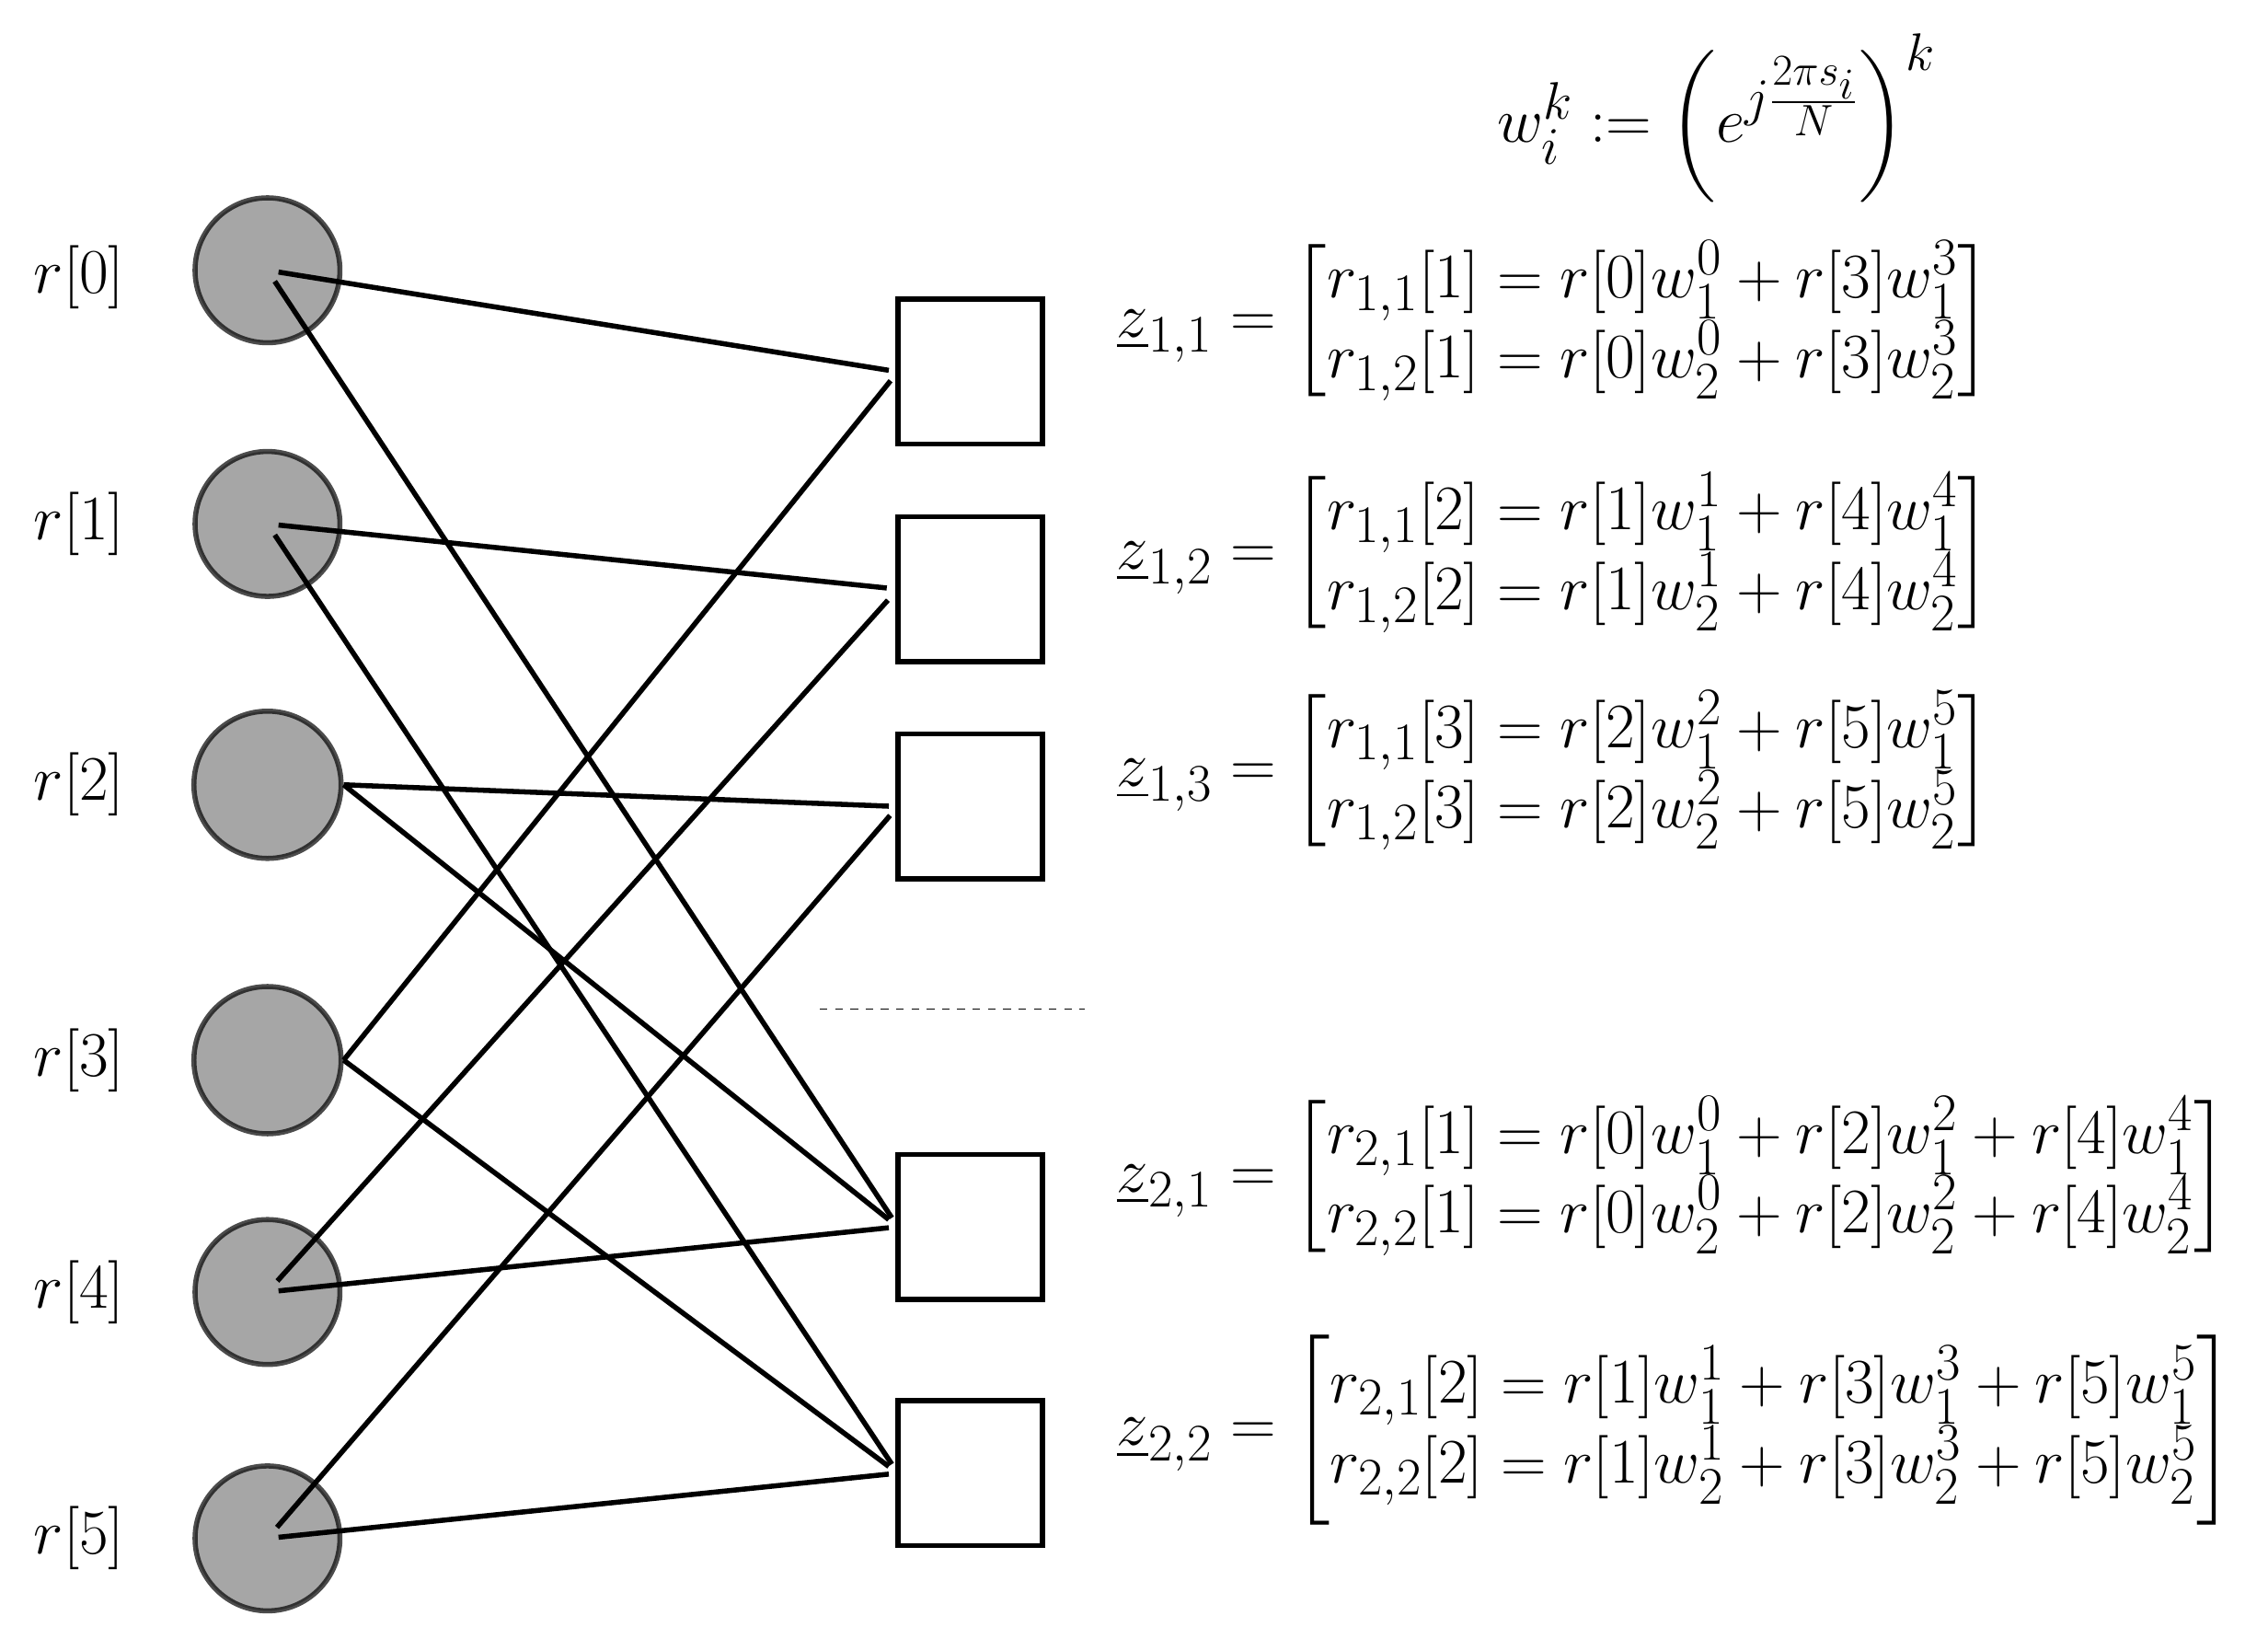
\begin{tikzpicture}

\definecolor{brightturquoise}{rgb}{0.03, 0.91, 0.87}
\definecolor{buff}{rgb}{0.94, 0.86, 0.51}
\definecolor{caribbeangreen}{rgb}{0.0, 0.8, 0.6}
\definecolor{celadon}{rgb}{0.67, 0.88, 0.69}
\definecolor{darktangerine}{rgb}{1.0, 0.66, 0.07}
\definecolor{darkviolet}{rgb}{0.58, 0.0, 0.83}
\definecolor{deepskyblue}{rgb}{0.0, 0.75, 1.0}
\definecolor{amber(sae/ece)}{rgb}{1.0, 0.49, 0.0}
\definecolor{antiquewhite}{rgb}{0.98, 0.92, 0.84}
\definecolor{applegreen}{rgb}{0.55, 0.71, 0.0}
\definecolor{babyblue}{rgb}{0.54, 0.81, 0.94}

\def\nodewidth{0.8in}
\tikzstyle{bit} = [circle, draw, thick,fill=gray,opacity=0.7,line width =2, minimum size=\nodewidth]

% Variable nodes 
\node[bit] (v6) at (-7,-6){};
\node[bit] (v5) at (-7,-2.2) {};
%\draw[thick,fill=gray,line width =2,opacity=0.7]  (-7,-2.2) node (v5) {} ellipse (1 and 1);
\draw [thick,fill=gray,line width =2,opacity=0.7]  (-7,1.4) node (v3) {} ellipse (1 and 1);
\draw  [thick,fill=gray,line width =2,opacity=0.7]  (-7,-9.2) node (v1) {} ellipse (1 and 1);
\draw  [thick,fill=gray,line width =2,opacity=0.7]  (-7,-12.6) node (v1_1) {} ellipse (1 and 1);
\draw  [thick,fill=gray,line width =2,opacity=0.7]  (-7,4.9) node (v1_2) {} ellipse (1 and 1);

%Check nodes
\draw [thick,line width =2] (1.7,4.5) rectangle (3.7,2.5);
\draw [thick,line width =2]  (1.7,1.5) node (v8) {} rectangle (3.7,-0.5);
\draw [thick,line width =2] (1.7,-1.5) rectangle (3.7,-3.5);
\draw [thick,line width =2] (1.7,-7.3) rectangle (3.7,-9.3);
\draw [thick,line width =2] (1.7,-10.7) rectangle (3.7,-12.7);

\node (v2) at (1.7,3.5) {};
\node (v4) at (1.7,-2.5) {};
\node (v7) at (1.7,-8.3) {};
\node (v9) at (1.7,-11.7) {};
\node (v10) at (0.5,-5.3) {};
\node (v11) at (4.4,-5.3) {};



\node at (-9.6,4.8) {\Huge $r[0]$};
\node at (-9.6,1.4) {\Huge $r[1]$};
\node at (-9.6,-2.2) {\Huge $r[2]$};
\node at (-9.6,-6) {\Huge $r[3]$};
\node at (-9.6,-9.2) {\Huge $r[4]$};
\node at (-9.6,-12.6) {\Huge $r[5]$};


\draw [dashed] (v10) edge (v11);
\node [anchor=west] at (4.6,4.2) {\Huge $ \zv_{1,1} = \begin{bmatrix}
	 r_{1,1}[1] = r[0] w_1^{0} + r[3] w_1^{3}  \\
	 r_{1,2}[1] = r[0] w_2^{0} + r[3] w_2^{3} \\
	 \end{bmatrix}$};

\node [anchor=west] at (4.6,1) {\Huge $  \zv_{1,2} = \begin{bmatrix}
	 r_{1,1}[2] = r[1] w_1^{1} + r[4] w_1^{4}\\
	 r_{1,2}[2] = r[1] w_2^{1} + r[4] w_2^{4}\\
	 \end{bmatrix}$};

\node [anchor=west] at (4.6,-2) {\Huge $  \zv_{1,3} = \begin{bmatrix}
	 r_{1,1}[3] = r[2] w_1^{2} + r[5] w_1^{5} \\
	 r_{1,2}[3] = r[2] w_2^{2} + r[5] w_2^{5} \\
	 \end{bmatrix}$};

\node [anchor=west] at (4.6,-7.6) {\Huge $  \zv_{2,1} = \begin{bmatrix}
	 r_{2,1}[1]= r[0] w_1^{0} + r[2] w_1^{2} + r[4] w_1^{4} \\
	 r_{2,2}[1] = r[0] w_2^{0} + r[2] w_2^{2} + r[4] w_2^{4}\\
	 \end{bmatrix}$};

\node [anchor=west] at (4.6,-11.1){\Huge $  \zv_{2,2} = \begin{bmatrix}
	 r_{2,1}[2] =  r[1] w_1^{1} + r[3] w_1^{3} + r[5] w_1^{5} \\ \vspace{3pt}
	 r_{2,2}[2] =  r[1] w_2^{1} + r[3] w_2^{3} + r[5] w_2^{5} \\
	 \end{bmatrix}$};


\draw[thick,line width =2]  (v1_2) edge (v2);
\draw[thick,line width =2]  (v1_2) edge (v7);

\draw[thick,line width =2]  (v3) edge (v9);
\draw[thick,line width =2]  (v5.east) edge (v4);
\node[thick,line width =2] (v12) at (1.7,0.5) {};
\draw[thick,line width =2]  (v3) edge (v12);
\draw[thick,line width =2]  (v5.east) edge (v7);

\draw[thick,line width =2]  (v6.east) edge (v2);
\draw[thick,line width =2]  (v1) edge (v12);
\draw[thick,line width =2]  (v1_1) edge (v4);
\draw[thick,line width =2]  (v6.east) edge (v9);
\draw [thick,line width =2] (v1_1) edge (v9);
\draw [thick,line width =2] (v1) edge (v7);
%\node at (6,7) {\color{blue} \Huge$w_j=e^{j \frac{2\pi s_{j}}{N} }$};
\node at (13,7) { \Huge $w_i^k := \left (  e^{j \frac{2 \pi s_i}{N}}\right )^{k}$};
\end{tikzpicture}
}	
			\end{center}	
			%\caption{Example of a Tanner graph formed in a RSIDFT framework with system parameters being $d=2$, $B=2$, $N=6$, $f_1 = 2$ and $f_2=3$. The variable nodes (colored gray circles) represent the cross-correlation vector $\rv$ and the bin nodes (uncolored white boxes) represent the binned observation vector $\zv_{i,k}$. The figure also illustrates the relationship between $\zv_{i,k}$ and $\rv$.}\label{fig:factorgraph}
		\end{figure}
	\column[]{0.33\columnwidth}
	    \begin{block}{Observations:}
	          $
	    		\zv_{i,k} = \begin{bmatrix}
	    		r_{i,1}[k]\\
	    		r_{i,2}[k]\\
	    		\vdots\\
	    		r_{i,B}[k]
	    		\end{bmatrix}^{T}
	    		$
	    	\end{block}
	    	\begin{block}{Decoding- 3 steps}	
	    		\begin{enumerate}
	    			\item Bin Classification
	    			\item Position Identification
	    			\item Peeling Process
	    		\end{enumerate}
	
	    \end{block}
	
		
\end{columns}
	
		
						
\end{frame}

\begin{frame}\frametitle{Decoder}

\only<1>{\begin{block}{Bin Classification}
		\begin{itemize}
			\item  Classify each check-node -  Zero-ton / Single-ton / Multi-ton
			\item  {\color{blue} Threshold constraints} on first observation $z_{i,k}[1] = z$
			\item  Threshold varies with $\eta$
			\begin{itemize}
				\item[-] different for exact($\eta=0$) and approximate matching
			\end{itemize}
		\end{itemize}
		\begin{align}
		\label{Eqn:BinClassifApprox} \nonumber
		\widehat{\mc{H}}_{i,j}=
		\begin{cases}
		\mc{H}_z &  	 z/M < \gamma_1\\
		\mc{H}_s &	  \gamma_1 < z/M < \gamma_2  \\
		\mc{H}_d  &    \gamma_2  < z/M <  \gamma_3\\
		\mc{H}_m &      z/M > \gamma_3\\
		\end{cases}
		\end{align}
		where $(\gamma_1,\gamma_2,\gamma_3)=(\frac{1-2\eta}{2},\frac{3-4\eta}{2},\frac{5-6\eta}{2})$
	\end{block}}
	
\only<2>{\vspace{-5pt} \begin{block}{Position Identification}
		\begin{itemize}
			\item 	{\color{blue}Observation:} 	\begin{align} \nonumber
			\label{Eqn:Generator Equation}
			\zv_{i,k}= \begin{bmatrix}
			1 & 1 & \ldots & 1 \\
			\omega^{k s_2} & \omega^{(k+f_i) s_2} & \ldots & \omega^{(k+(g_i-1)f_i) s_2}   \\
			\vdots & \vdots & \ddots & \vdots\\
			\omega^{k s_B} & \omega^{(k+f_i) s_B} & \ldots & \omega^{(k+(g_i-1)f_i) s_B} \\
			\end{bmatrix} \times
			\begin{bmatrix}
			r[k+(0)f_i] \\
			r[k+(1)f_i] \\
			\vdots\\
			r[k+(g_i-1)f_i]
			\end{bmatrix}
			\end{align}
			
			\item Column that gives {\color {blue} maximum correlation} with the observation\\
			{ \[\boxed{\hat{k} = \underset{k\in\{j+l f_i\}}{\arg \max}~~ \zv^{\dagger}_{i,j} \mathbf{W}[:,l]}\]}
		\end{itemize}
	
		\end{block}}

\only<3>{ {\Large \alert{Peeling Process:}}
	\begin{columns}
		\column[]{0.35\columnwidth}
	\begin{block}{Exact Matching}
			\begin{itemize}
				\item Remove a decoded variable node's contribution from {\color{blue}all participating bin nodes}
			\end{itemize}
	\end{block}
		\begin{block}{Approximate Matching}
			\begin{itemize}
				\item Remove a decoded variable node's contribution only from neighboring {\color{blue}single-tons and double-tons}
				 \item Avoid error propagation
			\end{itemize}
		\end{block}
		\column[]{0.65\columnwidth}
		\begin{figure}[h!]
			\begin{center}
				%		\includegraphics[height=7cm]{Figures/Factorgraph}
				\resizebox{1\textwidth}{!}{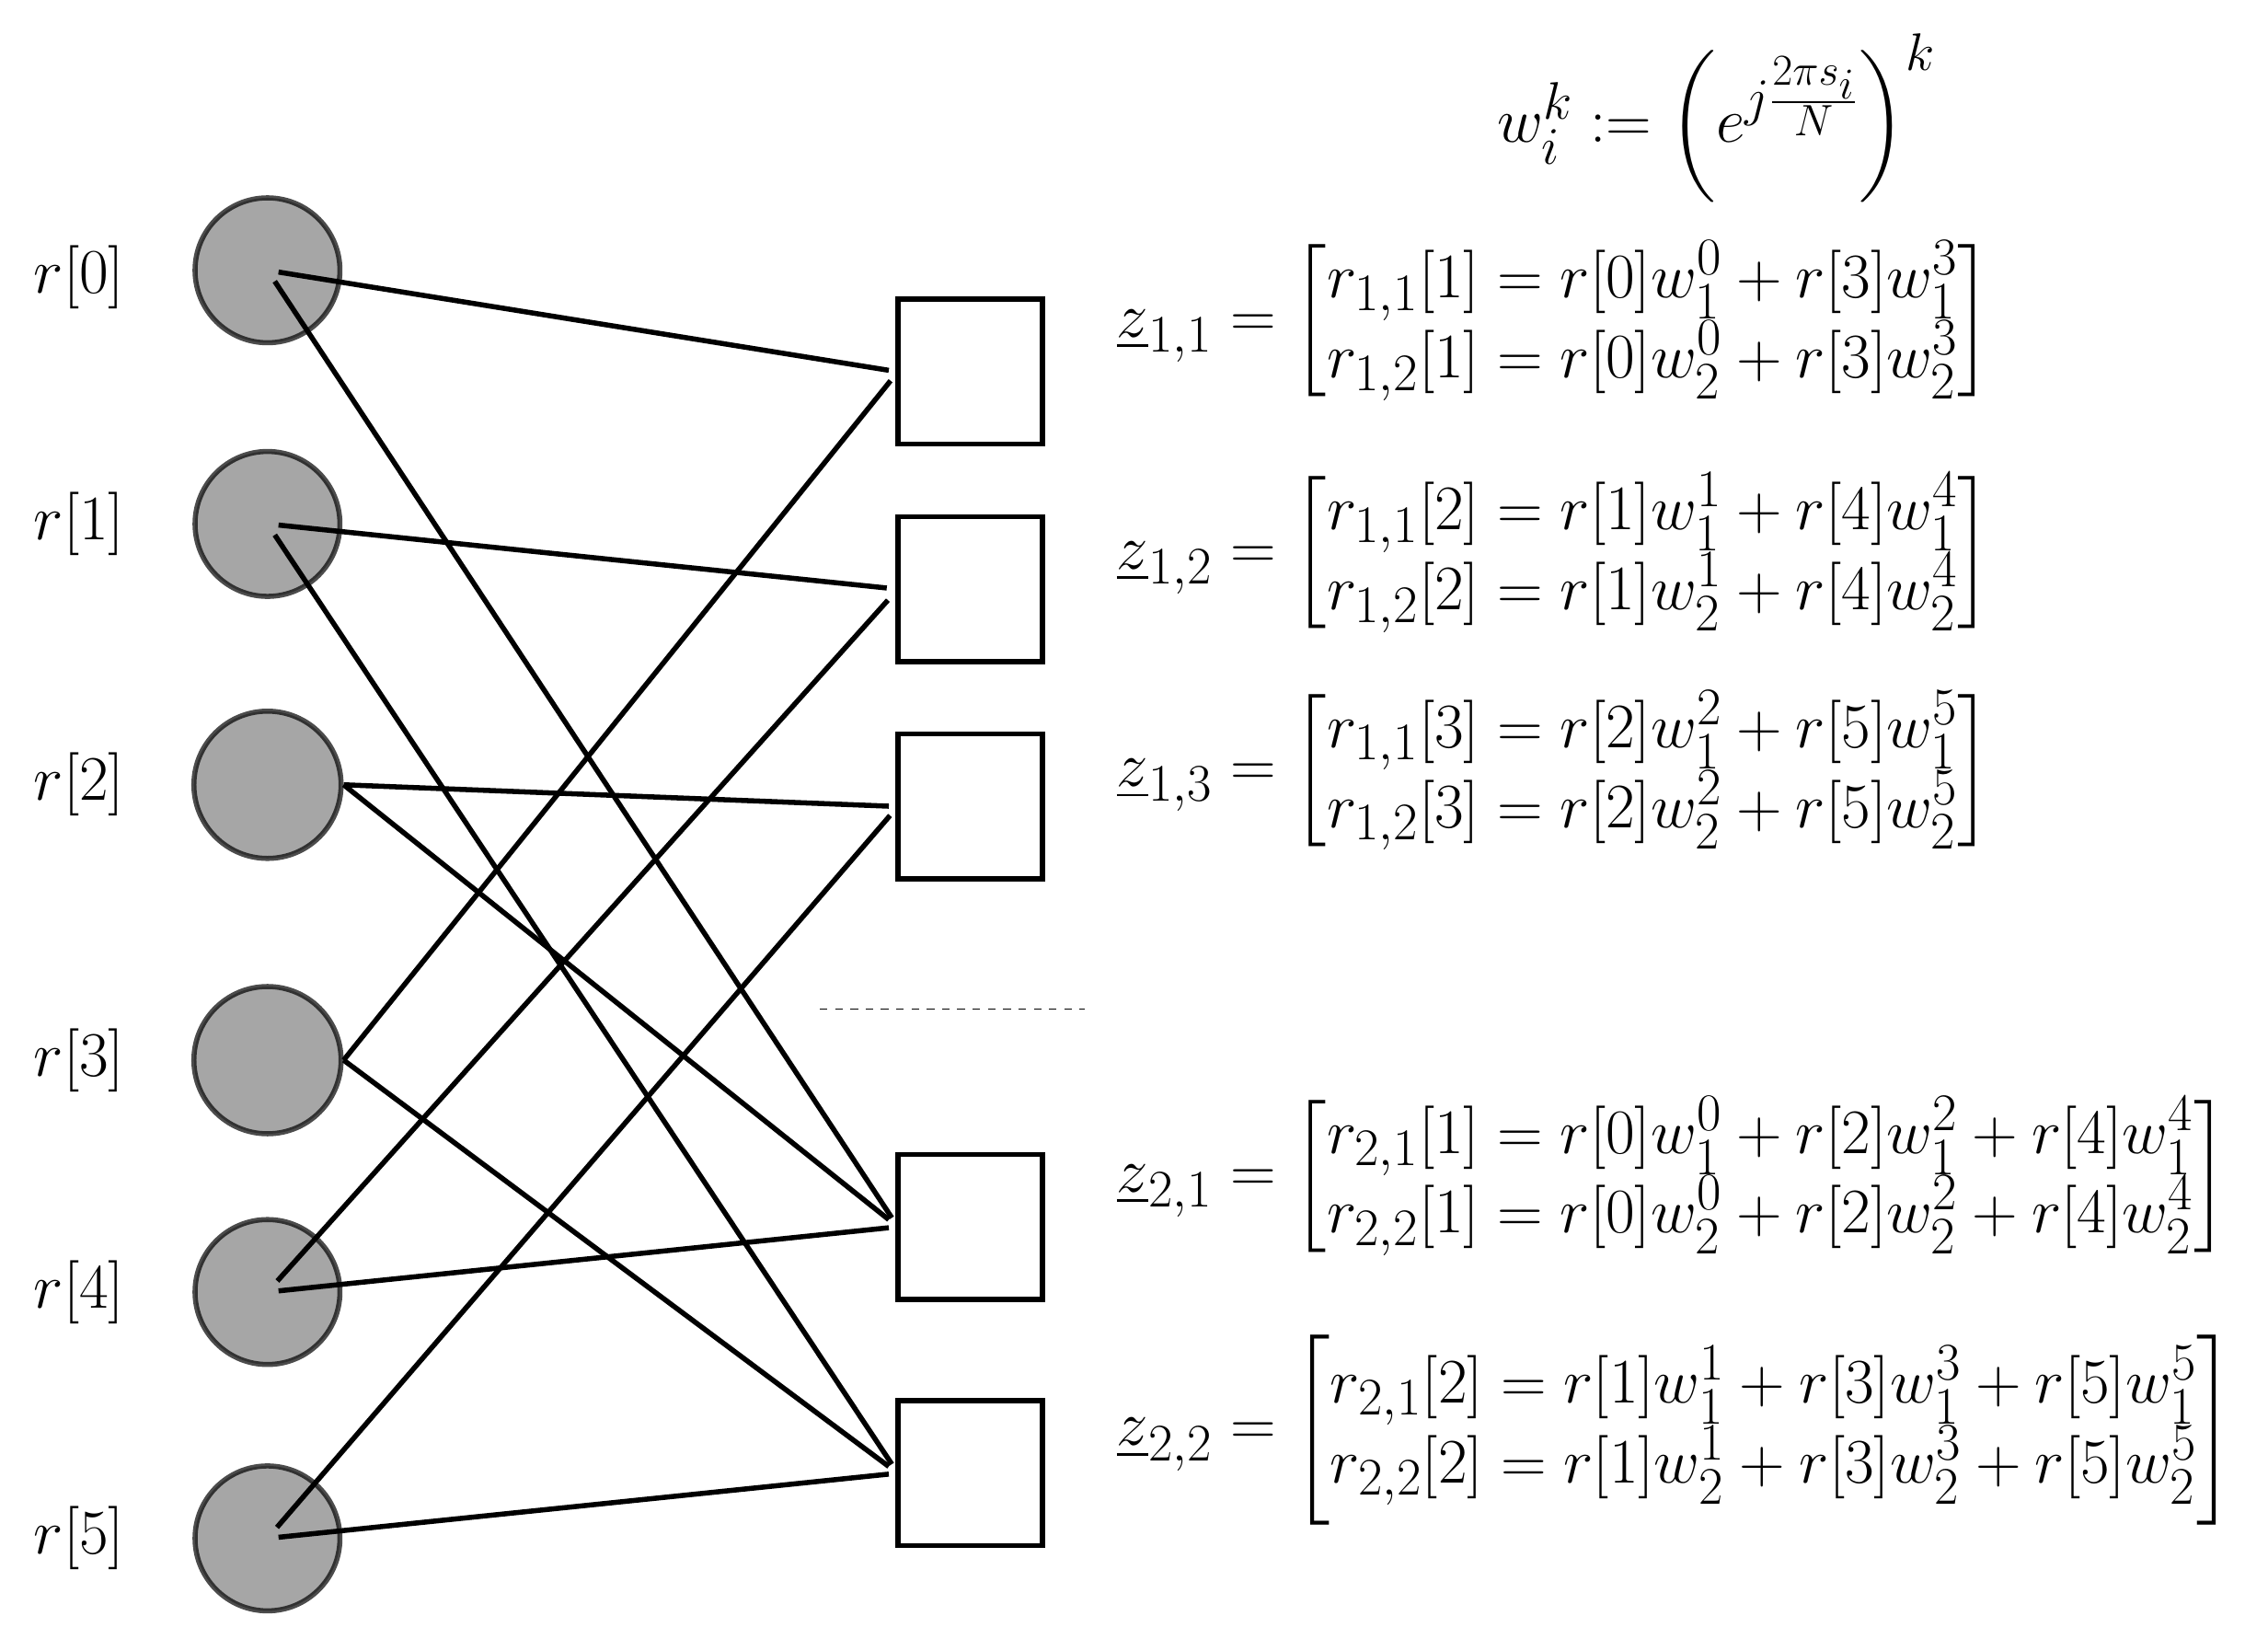
\begin{tikzpicture}

\definecolor{brightturquoise}{rgb}{0.03, 0.91, 0.87}
\definecolor{buff}{rgb}{0.94, 0.86, 0.51}
\definecolor{caribbeangreen}{rgb}{0.0, 0.8, 0.6}
\definecolor{celadon}{rgb}{0.67, 0.88, 0.69}
\definecolor{darktangerine}{rgb}{1.0, 0.66, 0.07}
\definecolor{darkviolet}{rgb}{0.58, 0.0, 0.83}
\definecolor{deepskyblue}{rgb}{0.0, 0.75, 1.0}
\definecolor{amber(sae/ece)}{rgb}{1.0, 0.49, 0.0}
\definecolor{antiquewhite}{rgb}{0.98, 0.92, 0.84}
\definecolor{applegreen}{rgb}{0.55, 0.71, 0.0}
\definecolor{babyblue}{rgb}{0.54, 0.81, 0.94}

\def\nodewidth{0.8in}
\tikzstyle{bit} = [circle, draw, thick,fill=gray,opacity=0.7,line width =2, minimum size=\nodewidth]

% Variable nodes 
\node[bit] (v6) at (-7,-6){};
\node[bit] (v5) at (-7,-2.2) {};
%\draw[thick,fill=gray,line width =2,opacity=0.7]  (-7,-2.2) node (v5) {} ellipse (1 and 1);
\draw [thick,fill=gray,line width =2,opacity=0.7]  (-7,1.4) node (v3) {} ellipse (1 and 1);
\draw  [thick,fill=gray,line width =2,opacity=0.7]  (-7,-9.2) node (v1) {} ellipse (1 and 1);
\draw  [thick,fill=gray,line width =2,opacity=0.7]  (-7,-12.6) node (v1_1) {} ellipse (1 and 1);
\draw  [thick,fill=gray,line width =2,opacity=0.7]  (-7,4.9) node (v1_2) {} ellipse (1 and 1);

%Check nodes
\draw [thick,line width =2] (1.7,4.5) rectangle (3.7,2.5);
\draw [thick,line width =2]  (1.7,1.5) node (v8) {} rectangle (3.7,-0.5);
\draw [thick,line width =2] (1.7,-1.5) rectangle (3.7,-3.5);
\draw [thick,line width =2] (1.7,-7.3) rectangle (3.7,-9.3);
\draw [thick,line width =2] (1.7,-10.7) rectangle (3.7,-12.7);

\node (v2) at (1.7,3.5) {};
\node (v4) at (1.7,-2.5) {};
\node (v7) at (1.7,-8.3) {};
\node (v9) at (1.7,-11.7) {};
\node (v10) at (0.5,-5.3) {};
\node (v11) at (4.4,-5.3) {};



\node at (-9.6,4.8) {\Huge $r[0]$};
\node at (-9.6,1.4) {\Huge $r[1]$};
\node at (-9.6,-2.2) {\Huge $r[2]$};
\node at (-9.6,-6) {\Huge $r[3]$};
\node at (-9.6,-9.2) {\Huge $r[4]$};
\node at (-9.6,-12.6) {\Huge $r[5]$};


\draw [dashed] (v10) edge (v11);
\node [anchor=west] at (4.6,4.2) {\Huge $ \zv_{1,1} = \begin{bmatrix}
	 r_{1,1}[1] = r[0] w_1^{0} + r[3] w_1^{3}  \\
	 r_{1,2}[1] = r[0] w_2^{0} + r[3] w_2^{3} \\
	 \end{bmatrix}$};

\node [anchor=west] at (4.6,1) {\Huge $  \zv_{1,2} = \begin{bmatrix}
	 r_{1,1}[2] = r[1] w_1^{1} + r[4] w_1^{4}\\
	 r_{1,2}[2] = r[1] w_2^{1} + r[4] w_2^{4}\\
	 \end{bmatrix}$};

\node [anchor=west] at (4.6,-2) {\Huge $  \zv_{1,3} = \begin{bmatrix}
	 r_{1,1}[3] = r[2] w_1^{2} + r[5] w_1^{5} \\
	 r_{1,2}[3] = r[2] w_2^{2} + r[5] w_2^{5} \\
	 \end{bmatrix}$};

\node [anchor=west] at (4.6,-7.6) {\Huge $  \zv_{2,1} = \begin{bmatrix}
	 r_{2,1}[1]= r[0] w_1^{0} + r[2] w_1^{2} + r[4] w_1^{4} \\
	 r_{2,2}[1] = r[0] w_2^{0} + r[2] w_2^{2} + r[4] w_2^{4}\\
	 \end{bmatrix}$};

\node [anchor=west] at (4.6,-11.1){\Huge $  \zv_{2,2} = \begin{bmatrix}
	 r_{2,1}[2] =  r[1] w_1^{1} + r[3] w_1^{3} + r[5] w_1^{5} \\ \vspace{3pt}
	 r_{2,2}[2] =  r[1] w_2^{1} + r[3] w_2^{3} + r[5] w_2^{5} \\
	 \end{bmatrix}$};


\draw[thick,line width =2]  (v1_2) edge (v2);
\draw[thick,line width =2]  (v1_2) edge (v7);

\draw[thick,line width =2]  (v3) edge (v9);
\draw[thick,line width =2]  (v5.east) edge (v4);
\node[thick,line width =2] (v12) at (1.7,0.5) {};
\draw[thick,line width =2]  (v3) edge (v12);
\draw[thick,line width =2]  (v5.east) edge (v7);

\draw[thick,line width =2]  (v6.east) edge (v2);
\draw[thick,line width =2]  (v1) edge (v12);
\draw[thick,line width =2]  (v1_1) edge (v4);
\draw[thick,line width =2]  (v6.east) edge (v9);
\draw [thick,line width =2] (v1_1) edge (v9);
\draw [thick,line width =2] (v1) edge (v7);
%\node at (6,7) {\color{blue} \Huge$w_j=e^{j \frac{2\pi s_{j}}{N} }$};
\node at (13,7) { \Huge $w_i^k := \left (  e^{j \frac{2 \pi s_i}{N}}\right )^{k}$};
\end{tikzpicture}
}	
			\end{center}
		\end{figure}
	\end{columns}}
\end{frame}

\begin{frame}{Error Analysis}
	
	\only<1,3>{\begin{block}{Error Events}
		\begin{itemize}\small
				\item {\color{blue}$\mathcal{E}_1${-\it Bin Classification}}: Bin is wrongly classified
				\item {\color{blue}$\mathcal{E}_2${-\it Pos. Identification}}: Position of singleton is identified wrongly, given a singleton
				\item {\color{blue}$\mathcal{E}_3${-\it Peeling Process}}: Peeling process fails to recover the $L$ significant correlation coefficients, given $\mbb{P}(\mc{E}_1)= \mbb{P}(\mc{E}_2)=0$
		\end{itemize}
	\end{block}
}
	\only<1>{\begin{block}{$\mathcal{E}_1${-\it Bin Classification}}
			\begin{figure}[t]
			\begin{center}
				\includegraphics[width=3.5in]{bin_statistics.png}
			\end{center}
		\end{figure}
		\vspace{-20pt}
		
		{\small \begin{align*}
			\mbb{P}[\mc{E}_1] & \leq & \mbb{P}[\mc{E}_1|\widehat{\mc{H}}_{i,j}=\mc{H}_z]~& + &
			\quad \mbb{P}[\mc{E}_1|\widehat{\mc{H}}_{i,j}=\mc{H}_s]~~~~~& + &
			\quad \mbb{P}[\mc{E}_1|\widehat{\mc{H}}_{i,j}=\mc{H}_d \cup \mc{H}_m]\\
			~& = & \mbb{P}[z[1]>\gamma_1] ~& + & (1- \mbb{P}[\gamma_1<z[1]<\gamma_2])  ~& + & \mbb{P}[z[1]<\gamma_2]~~~~~~
			\end{align*}
		}

			\vspace{-17pt}
	\end{block}
	}
	
	\only<2>{\begin{block}{$\mathcal{E}_2${-\it Pos. Identification}}
			\begin{itemize}
				\item $\underline{z} =  r[j_p] ~ \wv_{j_p}+ \sum_{k \neq p}n_k \wv_{j_k}$
				\item $\mbb{P}[\mc{E}_2] = \mbb{P}[\wv_{j_p}^{\dagger}\underline{z}< \wv_{j_k}^{\dagger}\underline{z}]$
				\item Mutual Incoherence property to bound the cross-correlation(noise) term
				  \begin{itemize}
				  	\item [-] $\log N$ measurements (shifts) suffices [PR2014]
				  \end{itemize}
			\end{itemize}
		     \end{block}
		
		\begin{block}{$\mathcal{E}_3${-\it Peeling Process}}
		\begin{itemize}
			\item Tools from Coding Theory to analyze Sparse Graph Codes
			\item Density Evolution to quantify Error Probability
			\item \# of check-nodes is a function of sparsity (query length)
			\item Exponentially decaying error probability- {\small R-FFAST and SAFFRON [PR2014,LPR2015]}
		\end{itemize}
		\end{block}
	}	
	
		\only<3>{\begin{block}{Error Probability}
			\begin{align*}
			\mbb{P}(\mathcal{E}_{\text{total}}) & \leq &  \mbb{P}(\mathcal{E}_1)~~~~~ & + & \mbb{P}(\mc{E}_2)~~~~~~~~ & + & \mbb{P}(\mc{E}_3)~~~~~~~~\\
			&\leq & 6e^{-\frac{N^{\mu+\alpha-1}(1-6\eta)^2}{16}}~ & + & 2e^{-N^{\mu+\alpha-1} ~ c_1(\eta)}~ & + &  e^{-c_3 N^{c_4\alpha}}
			\end{align*}
			\[\boxed{	\mbb{P}(\mathcal{E}_{\text{total}}) \rightarrow 0  ~~\text{if}~~  \alpha >1-\mu}\]
		\end{block}
	     }	
\end{frame}

\begin{frame}{Complexity Analysis}
	\begin{block}{Sample Complexity}
		\vspace{-10pt}
		\begin{align*}
		\text{Total \# of samples required (S)} &= O \left(dBN^{\alpha}\right) =   {\color{blue}O(N^{1-\mu}\log N)}
		\end{align*}
		
	\end{block}
	\begin{block}{Computational Complexity}
		\begin{equation*}\label{eqn:Rxy_fourier}
		\rv = \underset{\color{red}  \RNum{2} } {\mathcal{F}_{N}^{-1}} \ \{   \mathcal{F}_{N}\{\xv\}  \odot \ \underset{\color{red}  \RNum{1}  }{ \mathcal{F}_{N}\{\yv'\}}  \}
		\end{equation*}
		\vspace{-10pt}
	\begin{itemize}
		\item {\color{blue}Sketch of Query:}\\ \vspace{5pt}
	 {\small $C_{\color{red}\RNum{1}} \ = \  dB ~
	 ( \underset{\text{Folding} }{\underbrace{N^{\mu}}} + \ \
	 \underset{\text{Shorter FFTs} }{\underbrace{N^{\alpha} \ \log N^{\alpha}}} \ )
	 =  {\color{blue} O(\max(N^{1-\mu}\log^2 N ,N^{\mu}\log N)) }$}

		\item {\color{blue}RSIDFT:} \\	{\small$C_{\color{red} \RNum{2}} =  {d B}  \left (
			\underset{\text{Shorter IFFTs /block/stage} }{\underbrace{ O(N^{\alpha}  \log N^{\alpha})}} \hspace{-3pt}+ \underset{\text{Correlations} }{\underbrace{ L~N^{1-\alpha}}} \right ) = {\color{blue} O(\max(N^{1-\mu}\log^2 N ,N^{\mu+\lambda}\log N)) }$}
	\end{itemize}
	\vspace{10pt}	
	\[\boxed{C_{\text{total}} = \max(C_{\color{red} \text{ \RNum{1}}},C_{\color{red} \text{ \RNum{2}}}) = {\color{blue} O(\max(N^{1-\mu}\log^2 N ,N^{\mu+\lambda}\log N)) }}\]
		
	\end{block}
\end{frame}

\begin{frame}\frametitle{Simulation Results}
\only<1>{\begin{figure}[h!]
		\begin{center}
			
			\resizebox{0.7\textwidth}{!}{% This file was created by matlab2tikz.
%
%The latest updates can be retrieved from
%  http://www.mathworks.com/matlabcentral/fileexchange/22022-matlab2tikz-matlab2tikz
%where you can also make suggestions and rate matlab2tikz.
%
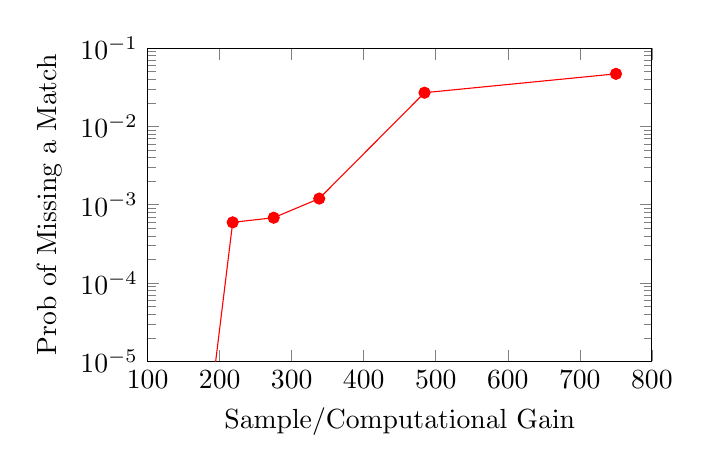
\begin{tikzpicture}

\begin{axis}[%
width=2.521in,
height=1.566in,
at={(0.758in,0.481in)},
scale only axis,
xmin=100,
xmax=800,
xlabel={Sample/Computational Gain},
ymode=log,
ymin=1e-05,
ymax=0.1,
yminorticks=true,
ylabel={Prob of Missing a Match},
axis background/.style={fill=white}
]
\addplot [color=red,solid,mark=*,mark options={solid},forget plot]
  table[row sep=crcr]{%
167.8088	1e-07\\
218.0519	0.0005965\\
274.9922	0.0006834\\
338.1745	0.0012\\
484.384	0.027\\
750.2035	0.047\\
};
\end{axis}
\end{tikzpicture}% }	
				\end{center}
			\caption{Plot of Probability of Missing a Match vs. Sample Gain for Exact Matching of a substring of length $M=10^5$($\mu=0.41$) from a equiprobable  binary \{+1,-1\} sequence of length $N= 10^{12}$, divided into $G=10^{5}$ blocks each of length $\tilde{N}=10^7$. The substring was simulated to repeat in $L=10^6$($\lambda=0.5$) locations uniformly at random.}
	
\end{figure}}

\only<2>{\begin{figure}[h!]
	\begin{center}
		\resizebox{0.7\textwidth}{!}{% This file was created by matlab2tikz.
%
%The latest updates can be retrieved from
%  http://www.mathworks.com/matlabcentral/fileexchange/22022-matlab2tikz-matlab2tikz
%where you can also make suggestions and rate matlab2tikz.
%
\begin{tikzpicture}

\begin{axis}[%
width=2.521in,
height=1.566in,
at={(0.758in,0.481in)},
scale only axis,
xmin=2,
xmax=18,
xlabel={Sample/Computational gain},
ymode=log,
ymin=1e-05,
ymax=1,
yminorticks=true,
ylabel={Prob of missing a match},
axis background/.style={fill=white}
]
\addplot [color=red,solid,mark=*,mark options={solid},forget plot]
  table[row sep=crcr]{%
2.0985	4e-07\\
3.2978	0.004\\
3.9974	0.004\\
4.7636	0.006\\
5.9963	0.017\\
7.3622	0.038\\
9.4944	0.054\\
17.4904	0.197\\
};
\end{axis}
\end{tikzpicture}% }	
	\end{center}
	\caption{Plot of Probability of Missing a Match vs. Sample Gain for Exact Matching of a substring of length $M=10^3$($\mu=0.25$) from a equiprobable  binary \{+1,-1\} sequence of length $N= 10^{12}$, divided into $G=10^{6}$ blocks each of length $\tilde{N}=10^6$. The substring was simulated to repeat in $L=10^6$($\lambda=0.5$) locations uniformly at random.}
	
\end{figure}}

\end{frame}	







%%%------------------------------------------			
%\begin{frame} \frametitle{Syndromes and decoding}
%%-----------------------------------------------------			
%\vspace*{-0.25in}
%\begin{figure}[t]
%			\centering
%            \resizebox{4.0in}{!}{\begin{tikzpicture}

%A matrix
\draw [fill=cyan, opacity=.2,rotate=90, thick]  (0.1,4.35) node (v1) {} rectangle (3.9,-3.75) node (v2) {};
\draw [thick,rotate=90,red] (v1) rectangle (3.9,3.1);
\draw [thick,rotate=90,red] (0.1,3.1) rectangle (3.9,1.8) node (v7) {};
\draw [thick,rotate=90,red] (0.1,-2.45) node (v6) {} rectangle (v2);
\draw[thick,red]  (v6) rectangle (1.15,3.9);
\draw[thick,red]  (v7) rectangle (-0.55,0.1);

\node at (-0.45,-1.4) {\huge \color{red} $ \underset{ \color{blue} ( Parity  \ checks)}{H_{ m \times n} }$};

% X vector
\draw [ thick] (5.85,5) rectangle (6.85,6);
\draw [thick] (6.85,5) rectangle (5.85,4);
\draw [thick] (5.85,4) rectangle (6.85,3);
\draw [] (5.85,3) node (v4) {} rectangle (6.85,-0.1) node (v5) {};
\draw [thick] (5.85,-0.1) rectangle (6.85,-1.1);
\draw [thick] (5.85,-1.1) rectangle (6.85,-2.1) node (v8) {};
\node at (6.45,-3.4) {\huge \color{red}  $\underset{\tiny \color{blue} (code \ vector)}{c_{n \times 1 }} $};
\node at (6.35,1.6) {\Large \bf \vdots};

\draw [thick] (v4) rectangle (6.85,2.1);
\draw [thick] (v5) rectangle (5.85,0.8);

% delta-x vector
\draw [ thick, fill=green] (9.4,5) rectangle (10.4,6);
\draw [thick] (10.4,5) rectangle (9.4,4);
\draw [thick, fill=green] (9.4,4) rectangle (10.4,3);
\draw [] (9.4,3) node (v4) {} rectangle (10.4,-0.1) node (v5) {};
\draw [thick, fill=green] (9.4,-0.1) rectangle (10.4,-1.1);
\draw [thick] (9.4,-1.1) rectangle (10.4,-2.1);
\node at (10,-3.4) {\huge \color{red}  $\underset{\color{black}{t-sparse}}{\underset{\tiny \color{blue} (error \ vector)}{e}} $};
\node at (9.9,1.6) {\Large \bf \vdots};
\node at (4.8,2.1) {\bf \Huge $\times$};
\draw [thick] (v4) rectangle (10.4,2.1);
\draw [thick] (v5) rectangle (9.4,0.8);

\node at (8.2,2) {\Huge \bf $+$};

\node at (9.9,5.5) {\color{red} \huge $ e_i$ };
\node at (9.9,3.5) {\color{red} \huge $ e_j$};
\node at (9.9,-0.55) {\color{red} \huge $ e_t$};

% y







\node at (15.9,1.6) {\bf \vdots};

\node at (11.8,2) {\Huge = };
\node at (15.8,-0.65) {\color{red} \huge $y_{m \times 1}$};
\node [align=left, text width =3.5cm] at (16.5,-2.15) {\Large  \color{blue} Syndromes};

\node at (0.3,2.45) {\Huge \bf $\cdots$};



% b_k

\draw [thick] (15.4,4.1) node (v3) {} rectangle (16.4,3.1);
\draw [thick] (15.4,3.1) rectangle (16.4,2.1);
\draw [thick] (15.4,2.1) rectangle (16.4,1);
\draw [thick] (15.4,1) rectangle (16.4,0);
\draw[fill=red, opacity=0.2]  (v3) rectangle (16.4,0);
\node at (-1.35,1.6) { \color{blue}\Large  \bf  \vdots};

\draw [dashed,blue] (-4.35,3.9) rectangle (3.75,3);
\draw [dashed,blue] (-4.35,3) rectangle (3.75,2);
\draw[dashed,blue]  (v1) rectangle (3.75,1);
\node at (-3.85,4.5) {\huge \bf  \color{red} $h_1$};
\node at (-2.4,4.5) {\huge \bf \color{red} $h_2$};
\node at (-1.25,4.5) {\huge \bf  \color{red} $h_i$};
\node at (0.25,4.5) {\huge \bf  \color{red} $\cdots$};
\node at (1.8,4.5) {\huge \bf  \color{red} $h_{n-1}$};
\node at (3.15,4.5) {\huge \bf  \color{red} $h_n$};

\node at (9.9,4.55) {\large \bf \vdots};


\node at (13.45,2) {\bf \Huge $0$};
\node at (14.45,2) {\huge \bf +};

\draw [fill=orange, opacity=0.5] (v8) rectangle (5.85,6);
\end{tikzpicture} }
%			%\includegraphics[width=4.0in]{./Figures/A_times_X_columns_coding.pdf}
%		\end{figure}
%\pause
%\begin{itemize}
%\item Syndrome : Linear combination of $\underline{h}_i$s, i.e., $\underline{y} = e_i \hv_i \oplus e_j \hv_j \oplus e_t \hv_t$
%\item Decoding : Find min weight $\underline{e}$ : $\underline{y} = e_i \hv_i \oplus e_j \hv_j \oplus e_t \hv_t$
%\end{itemize}
%\pause
%\begin{block}{\alert{Coding theory deals with the construction of $\mathbf{H}$ and efficient decoding algorithms, i.e., given a linear combination of the columns of $\mathbf{H}$, it develops tools to determine a sparse $\underline{e}$ }}\end{block}
%\end{frame}
%%------------------------------------------			
%\begin{frame} \frametitle{Syndrome source coding}
%%\begin{block}{Compression of a $p-$ary source}
%%\[
%%\begin{bmatrix}
%%y_1\\
%%\vdots\\
%%y_m\\
%%\end{bmatrix}
%%=
%%\begin{bmatrix}
%%  1 & 1 & 1 & \ldots & 1 \\
%%  1 & W & W^2 & \ldots & W^{n-1} \\
%%  1 & W^2 & W^4 & \ldots & W^{2n-2} \\
%%  \vdots & \vdots & \vdots & \vdots & \vdots \\
%%  1 & W^{2t-1} & W^{4t-2} & \ldots & W^{(2t-1)(n-1)}\\
%%\end{bmatrix}
%%\begin{bmatrix}
%%0\\
%%\vdots\\
%%x_1\\
%%\vdots \\
%%x_{k}\\
%%\vdots\\
%%0\\
%%\end{bmatrix}
%%\]
%%\end{block}
%
%\resizebox{4.0in}{!}{\begin{tikzpicture}

%A matrix
\begin{scope}[shift={(2,0)}]
\draw [fill=cyan, opacity=0.2,rotate=90, thick]  (0.1,4.35) node (v1) {} rectangle (3.9,-3.75) node (v2) {};
\draw [thick,rotate=90,red] (v1) rectangle (3.9,3.1);
\draw [thick,rotate=90,red] (0.1,3.1) rectangle (3.9,1.8) node (v7) {};
\draw [thick,rotate=90,red] (0.1,-2.45) node (v6) {} rectangle (v2);
\draw[thick,red]  (v6) rectangle (1.15,3.9);
\draw[thick,red]  (v7) rectangle (-0.55,0.1);
\node at (-0.45,-1.4) {\huge \color{red} $ \underset{ \color{blue} ( Parity  \ check \ matrix )}{H_{ m \times n} }$};
\node at (4.8,2.1) {\bf \Huge $\times$};
\node at (0.3,2.45) {\Huge \bf $\cdots$};
\node at (-1.35,1.6) { \color{blue}\Large  \bf  \vdots};
\draw [dashed,blue] (-4.35,3.9) rectangle (3.75,3);
\draw [dashed,blue] (-4.35,3) rectangle (3.75,2);
\draw[dashed,blue]  (v1) rectangle (3.75,1);
\node at (-3.85,4.5) {\huge \bf  \color{red} $h_1$};
\node at (-2.4,4.5) {\huge \bf \color{red} $h_2$};
\node at (-1.25,4.5) {\huge \bf  \color{red} $h_i$};
\node at (0.25,4.5) {\huge \bf  \color{red} $\cdots$};
\node at (1.8,4.5) {\huge \bf  \color{red} $h_{n-1}$};
\node at (3.15,4.5) {\huge \bf  \color{red} $h_n$};

\end{scope}










% X vector
%\draw [ thick] (5.85,5) rectangle (6.85,6);
%\draw [thick] (6.85,5) rectangle (5.85,4);
%\draw [thick] (5.85,4) rectangle (6.85,3);
%\draw [] (5.85,3) node (v4) {} rectangle (6.85,-0.1) node (v5) {};
%\draw [thick] (5.85,-0.1) rectangle (6.85,-1.1);
%\draw [thick] (5.85,-1.1) rectangle (6.85,-2.1) node (v8) {};
%\node at (6.45,-3.4) {\huge \color{red}  $\underset{\tiny \color{blue} (code \ vector)}{c_{n \times 1 }} $};
%\node at (6.35,1.6) {\Large \bf \vdots};
%
%\draw [thick] (v4) rectangle (6.85,2.1);
%\draw [thick] (v5) rectangle (5.85,0.8);

% delta-x vector
\draw [ thick, fill=green] (9.4,5) rectangle (10.4,6);
\draw [thick] (10.4,5) rectangle (9.4,4);
\draw [thick, fill=green] (9.4,4) rectangle (10.4,3);
\draw [] (9.4,3) node (v4) {} rectangle (10.4,-0.1) node (v5) {};
\draw [thick, fill=green] (9.4,-0.1) rectangle (10.4,-1.1);
\draw [thick] (9.4,-1.1) rectangle (10.4,-2.1);
\node at (10,-3.4) {\huge \color{red}  $\underset{\color{black}{t-sparse}}{\underset{\tiny \color{blue} (Source \ vector)}{x}} $};
\node at (9.9,1.6) {\Large \bf \vdots};

\draw [thick] (v4) rectangle (10.4,2.1);
\draw [thick] (v5) rectangle (9.4,0.8);

%\node at (8.2,2) {\Huge \bf $+$};

\node at (9.9,5.5) {\color{red} \huge $ x_1$ };
\node at (9.9,3.5) {\color{red} \huge $ x_i$};
\node at (9.9,-0.55) {\color{red} \huge $ x_t$};

% y

\begin{scope}[shift={(-1,0)}]
\node at (15.9,1.6) {\bf \vdots};
\node at (15.8,-0.65) {\color{red} \huge $y_{m \times 1}$};
\node [align=left, text width =3.5cm] at (16.5,-2) {\Large  \color{blue} Syndromes};
\draw [thick] (15.4,4.1) node (v3) {} rectangle (16.4,3.1);
\draw [thick] (15.4,3.1) rectangle (16.4,2.1);
\draw [thick] (15.4,2.1) rectangle (16.4,1);
\draw [thick] (15.4,1) rectangle (16.4,0);
\draw[fill=red, opacity=0.2]  (v3) rectangle (16.4,0);

\end{scope}


\node at (11.8,2) {\Huge = };







% b_k



















\node at (9.9,4.55) {\large \bf \vdots};


%\node at (13.45,2) {\bf \Huge $0$};
%\node at (14.45,2) {\huge \bf +};
%
%\draw [fill=orange, opacity=0.5] (v8) rectangle (5.85,6);


\end{tikzpicture}
}
%
%\begin{block}{Compression of a sparse binary source}
%\begin{itemize}
%\item Compressed version is the syndrome $\yv$
%\item Reconstruction is the same as decoding
%\item Similar to the canonical sparse recovery problem
%\end{itemize}
%\end{block}
%\end{frame}
%%--------------------------------------------------------------------------------------
%\begin{frame}{Syndrome source coding}
%
%\begin{columns}
%\column{0.5\textwidth}
%\begin{center}
%  \includegraphics[width=2.0in,angle=-90]{./Figures/syndromesourcecoding2_1}
%\end{center}
%\begin{itemize}
%  \item $H \underline{x} = 0$
%  \item Receive - $\underline{r} = \underline{x} \oplus \underline{e}$
%  \item $H \underline{r} = H \underline{e} = \underline{y}$
%  \item Recover $\xv$ and sparse $\ev$
%\end{itemize}
%\column{0.5\textwidth}
%\begin{center}
%  \includegraphics[width=2.0in,angle=-90]{./Figures/syndromesourcecoding2_2}
%\end{center}
%\begin{itemize}
%  \item $H \underline{s} = \underline{y}$
%  \item Set $\underline{r} = 0 $ (Let a genie add $\underline{x}$ to $\underline{r}$)
%  \item $\underline{y}$ is given to the decoder
%  \item Recover sparse $\sv$
%\end{itemize}
%\end{columns}
%\end{frame}
%------------------------------------------			
\begin{frame} \frametitle{Syndromes and decoding}
%-----------------------------------------------------			
\vspace*{-0.25in}
\begin{figure}[t]
			\centering
            \resizebox{4.0in}{!}{\begin{tikzpicture}

%A matrix
\draw [fill=cyan, opacity=.2,rotate=90, thick]  (0.1,4.35) node (v1) {} rectangle (3.9,-3.75) node (v2) {};
\draw [thick,rotate=90,red] (v1) rectangle (3.9,3.1);
\draw [thick,rotate=90,red] (0.1,3.1) rectangle (3.9,1.8) node (v7) {};
\draw [thick,rotate=90,red] (0.1,-2.45) node (v6) {} rectangle (v2);
\draw[thick,red]  (v6) rectangle (1.15,3.9);
\draw[thick,red]  (v7) rectangle (-0.55,0.1);

\node at (-0.45,-1.4) {\huge \color{red} $ \underset{ \color{blue} ( Parity  \ checks)}{H_{ m \times n} }$};

% X vector
\draw [ thick] (5.85,5) rectangle (6.85,6);
\draw [thick] (6.85,5) rectangle (5.85,4);
\draw [thick] (5.85,4) rectangle (6.85,3);
\draw [] (5.85,3) node (v4) {} rectangle (6.85,-0.1) node (v5) {};
\draw [thick] (5.85,-0.1) rectangle (6.85,-1.1);
\draw [thick] (5.85,-1.1) rectangle (6.85,-2.1) node (v8) {};
\node at (6.45,-3.4) {\huge \color{red}  $\underset{\tiny \color{blue} (code \ vector)}{c_{n \times 1 }} $};
\node at (6.35,1.6) {\Large \bf \vdots};

\draw [thick] (v4) rectangle (6.85,2.1);
\draw [thick] (v5) rectangle (5.85,0.8);

% delta-x vector
\draw [ thick, fill=green] (9.4,5) rectangle (10.4,6);
\draw [thick] (10.4,5) rectangle (9.4,4);
\draw [thick, fill=green] (9.4,4) rectangle (10.4,3);
\draw [] (9.4,3) node (v4) {} rectangle (10.4,-0.1) node (v5) {};
\draw [thick, fill=green] (9.4,-0.1) rectangle (10.4,-1.1);
\draw [thick] (9.4,-1.1) rectangle (10.4,-2.1);
\node at (10,-3.4) {\huge \color{red}  $\underset{\color{black}{t-sparse}}{\underset{\tiny \color{blue} (error \ vector)}{e}} $};
\node at (9.9,1.6) {\Large \bf \vdots};
\node at (4.8,2.1) {\bf \Huge $\times$};
\draw [thick] (v4) rectangle (10.4,2.1);
\draw [thick] (v5) rectangle (9.4,0.8);

\node at (8.2,2) {\Huge \bf $+$};

\node at (9.9,5.5) {\color{red} \huge $ e_i$ };
\node at (9.9,3.5) {\color{red} \huge $ e_j$};
\node at (9.9,-0.55) {\color{red} \huge $ e_t$};

% y







\node at (15.9,1.6) {\bf \vdots};

\node at (11.8,2) {\Huge = };
\node at (15.8,-0.65) {\color{red} \huge $y_{m \times 1}$};
\node [align=left, text width =3.5cm] at (16.5,-2.15) {\Large  \color{blue} Syndromes};

\node at (0.3,2.45) {\Huge \bf $\cdots$};



% b_k

\draw [thick] (15.4,4.1) node (v3) {} rectangle (16.4,3.1);
\draw [thick] (15.4,3.1) rectangle (16.4,2.1);
\draw [thick] (15.4,2.1) rectangle (16.4,1);
\draw [thick] (15.4,1) rectangle (16.4,0);
\draw[fill=red, opacity=0.2]  (v3) rectangle (16.4,0);
\node at (-1.35,1.6) { \color{blue}\Large  \bf  \vdots};

\draw [dashed,blue] (-4.35,3.9) rectangle (3.75,3);
\draw [dashed,blue] (-4.35,3) rectangle (3.75,2);
\draw[dashed,blue]  (v1) rectangle (3.75,1);
\node at (-3.85,4.5) {\huge \bf  \color{red} $h_1$};
\node at (-2.4,4.5) {\huge \bf \color{red} $h_2$};
\node at (-1.25,4.5) {\huge \bf  \color{red} $h_i$};
\node at (0.25,4.5) {\huge \bf  \color{red} $\cdots$};
\node at (1.8,4.5) {\huge \bf  \color{red} $h_{n-1}$};
\node at (3.15,4.5) {\huge \bf  \color{red} $h_n$};

\node at (9.9,4.55) {\large \bf \vdots};


\node at (13.45,2) {\bf \Huge $0$};
\node at (14.45,2) {\huge \bf +};

\draw [fill=orange, opacity=0.5] (v8) rectangle (5.85,6);
\end{tikzpicture} }
			%\includegraphics[width=4.0in]{./Figures/A_times_X_columns_coding.pdf}
		\end{figure}
\pause
\begin{itemize}
\item Syndrome : Linear combination of $\underline{h}_i$s, i.e., $\underline{y} = e_i \hv_i \oplus e_j \hv_j \oplus e_t \hv_t$
\item Decoding : Find min weight $\underline{e}$ : $\underline{y} = e_i \hv_i \oplus e_j \hv_j \oplus e_t \hv_t$
\end{itemize}
\pause
\begin{block}{\alert{Coding theory deals with the construction of $\mathbf{H}$ and efficient decoding algorithms, i.e., given a linear combination of the columns of $\mathbf{H}$, it develops tools to determine a sparse $\underline{e}$ }}\end{block}
\end{frame}
%------------------------------------------			
\begin{frame} \frametitle{Syndrome source coding}
%\begin{block}{Compression of a $p-$ary source}
%\[
%\begin{bmatrix}
%y_1\\
%\vdots\\
%y_m\\
%\end{bmatrix}
%=
%\begin{bmatrix}
%  1 & 1 & 1 & \ldots & 1 \\
%  1 & W & W^2 & \ldots & W^{n-1} \\
%  1 & W^2 & W^4 & \ldots & W^{2n-2} \\
%  \vdots & \vdots & \vdots & \vdots & \vdots \\
%  1 & W^{2t-1} & W^{4t-2} & \ldots & W^{(2t-1)(n-1)}\\
%\end{bmatrix}
%\begin{bmatrix}
%0\\
%\vdots\\
%x_1\\
%\vdots \\
%x_{k}\\
%\vdots\\
%0\\
%\end{bmatrix}
%\]
%\end{block}

\resizebox{4.0in}{!}{\begin{tikzpicture}

%A matrix
\begin{scope}[shift={(2,0)}]
\draw [fill=cyan, opacity=0.2,rotate=90, thick]  (0.1,4.35) node (v1) {} rectangle (3.9,-3.75) node (v2) {};
\draw [thick,rotate=90,red] (v1) rectangle (3.9,3.1);
\draw [thick,rotate=90,red] (0.1,3.1) rectangle (3.9,1.8) node (v7) {};
\draw [thick,rotate=90,red] (0.1,-2.45) node (v6) {} rectangle (v2);
\draw[thick,red]  (v6) rectangle (1.15,3.9);
\draw[thick,red]  (v7) rectangle (-0.55,0.1);
\node at (-0.45,-1.4) {\huge \color{red} $ \underset{ \color{blue} ( Parity  \ check \ matrix )}{H_{ m \times n} }$};
\node at (4.8,2.1) {\bf \Huge $\times$};
\node at (0.3,2.45) {\Huge \bf $\cdots$};
\node at (-1.35,1.6) { \color{blue}\Large  \bf  \vdots};
\draw [dashed,blue] (-4.35,3.9) rectangle (3.75,3);
\draw [dashed,blue] (-4.35,3) rectangle (3.75,2);
\draw[dashed,blue]  (v1) rectangle (3.75,1);
\node at (-3.85,4.5) {\huge \bf  \color{red} $h_1$};
\node at (-2.4,4.5) {\huge \bf \color{red} $h_2$};
\node at (-1.25,4.5) {\huge \bf  \color{red} $h_i$};
\node at (0.25,4.5) {\huge \bf  \color{red} $\cdots$};
\node at (1.8,4.5) {\huge \bf  \color{red} $h_{n-1}$};
\node at (3.15,4.5) {\huge \bf  \color{red} $h_n$};

\end{scope}










% X vector
%\draw [ thick] (5.85,5) rectangle (6.85,6);
%\draw [thick] (6.85,5) rectangle (5.85,4);
%\draw [thick] (5.85,4) rectangle (6.85,3);
%\draw [] (5.85,3) node (v4) {} rectangle (6.85,-0.1) node (v5) {};
%\draw [thick] (5.85,-0.1) rectangle (6.85,-1.1);
%\draw [thick] (5.85,-1.1) rectangle (6.85,-2.1) node (v8) {};
%\node at (6.45,-3.4) {\huge \color{red}  $\underset{\tiny \color{blue} (code \ vector)}{c_{n \times 1 }} $};
%\node at (6.35,1.6) {\Large \bf \vdots};
%
%\draw [thick] (v4) rectangle (6.85,2.1);
%\draw [thick] (v5) rectangle (5.85,0.8);

% delta-x vector
\draw [ thick, fill=green] (9.4,5) rectangle (10.4,6);
\draw [thick] (10.4,5) rectangle (9.4,4);
\draw [thick, fill=green] (9.4,4) rectangle (10.4,3);
\draw [] (9.4,3) node (v4) {} rectangle (10.4,-0.1) node (v5) {};
\draw [thick, fill=green] (9.4,-0.1) rectangle (10.4,-1.1);
\draw [thick] (9.4,-1.1) rectangle (10.4,-2.1);
\node at (10,-3.4) {\huge \color{red}  $\underset{\color{black}{t-sparse}}{\underset{\tiny \color{blue} (Source \ vector)}{x}} $};
\node at (9.9,1.6) {\Large \bf \vdots};

\draw [thick] (v4) rectangle (10.4,2.1);
\draw [thick] (v5) rectangle (9.4,0.8);

%\node at (8.2,2) {\Huge \bf $+$};

\node at (9.9,5.5) {\color{red} \huge $ x_1$ };
\node at (9.9,3.5) {\color{red} \huge $ x_i$};
\node at (9.9,-0.55) {\color{red} \huge $ x_t$};

% y

\begin{scope}[shift={(-1,0)}]
\node at (15.9,1.6) {\bf \vdots};
\node at (15.8,-0.65) {\color{red} \huge $y_{m \times 1}$};
\node [align=left, text width =3.5cm] at (16.5,-2) {\Large  \color{blue} Syndromes};
\draw [thick] (15.4,4.1) node (v3) {} rectangle (16.4,3.1);
\draw [thick] (15.4,3.1) rectangle (16.4,2.1);
\draw [thick] (15.4,2.1) rectangle (16.4,1);
\draw [thick] (15.4,1) rectangle (16.4,0);
\draw[fill=red, opacity=0.2]  (v3) rectangle (16.4,0);

\end{scope}


\node at (11.8,2) {\Huge = };







% b_k



















\node at (9.9,4.55) {\large \bf \vdots};


%\node at (13.45,2) {\bf \Huge $0$};
%\node at (14.45,2) {\huge \bf +};
%
%\draw [fill=orange, opacity=0.5] (v8) rectangle (5.85,6);


\end{tikzpicture}
}

\begin{block}{Compression of a sparse binary source}
\begin{itemize}
\item Compressed version is the syndrome $\yv$
\item Reconstruction is the same as decoding
\item Similar to the canonical sparse recovery problem
\end{itemize}
\end{block}
\end{frame}
%------------------------------------------------------------------------------
\begin{frame}\frametitle{Review of primitives}
\begin{itemize}
\item Idea of a check node or a measurement node which is a function of some symbols
\item Singleton detection - be able to identify one non-zero symbol
\item Peeling - if we know some symbols, be able to remove and adjust measurement
\end{itemize}
\end{frame}
%------------------------------------------------------------------------------
\begin{frame}{Application 3}
\end{frame}
%------------------------------------------------------
\begin{frame} \frametitle{Compressed sensing}
%-----------------------------------------------------
\vspace*{-0.2in}
\begin{figure}[t]
\centering
\includegraphics[width=2.75in]{./Figures/A_times_X_CS.pdf}
\end{figure}
\vspace*{-0.2in}
\begin{block}{Classical compressed sensing}
\begin{itemize}
\item $\xv$ is a $K$-sparse vector over $\mathbb{R}$ or $\mathbb{C}$
\item We `compress' $\xv$ by storing only $\yv = \mathbf{A} \ \xv$
\item Reconstruction - Solve $\hat{\xv} = \arg \min ||\zv||_0 : \yv = \mathbf{A} \zv$
\item CS - Solve $\hat{\xv} = \arg \min ||\zv||_1 : \yv = \mathbf{A} \zv$
\end{itemize}
\end{block}
\pause
\begin{block}{Coding theoretic approach - syndrome source coding over complex numbers}
\begin{itemize}

\item Sensing matrix $\mathbf{A} \Leftrightarrow $ Parity check matrix $\mathbf{H}$
\end{itemize}
\end{block}
\end{frame}		
%-------------------------------------------------------			
\begin{frame} \frametitle{Data stream computing}
%---------------------------------------------------------
\vspace*{-0.1in}
\begin{block}{Problem - consider a router in a large network}
\begin{itemize}
\item Count the number of packets from source $i$ to destination $j$, say $x_{ij}$
\item Data vector is huge, $n = 2^{64}$
\item Heavy hitters - only a few of them are large
\end{itemize}
\end{block}

\vspace*{-0.1in}
\begin{figure}[t]
		\centering
		\includegraphics[width=3.0in]{./Figures/A_times_X_columns.pdf}
	\end{figure}
\vspace*{-0.2in}
\begin{block}{Keep only a low dimensional ($m \ll n$) sketch of $x$}	
\begin{itemize}
\item {\color{blue}$\yv_{m \times 1} = \mathbf{A} \xv \Leftrightarrow$} Syndrome, $x_{i,j} \in \mathbb{Z}^+$
\item Reconstruction is same as decoding
\end{itemize}	
\end{block}	

\end{frame}

%------------------------------------------------------------------
\begin{frame}\frametitle{Incremental updates}

	\begin{figure}[t]
		\centering
		\includegraphics[width=4.7in]{./Figures/A_times_X_columns_Stream_inc.pdf}
	\end{figure}

\begin{block}{}

Sketch $y$ {\color{blue} supports incremental updates} to $x$ as the sketching procedure is linear. \\
\centering{\color{blue}$x+ \Delta_i \rightarrow y + A\Delta_i$}\\ (adding $i$th column vector of $A$ to existing sketch)

\end{block}				
	
	
%								\begin{block}{Objective}
%					
%					\begin{itemize}
%						
%						\item Design the {\color{blue}sketching matrix} $A$ that offers {\color{blue} high compression rates} (smaller $m$)
%						\item Design a {\color{blue} less-complex decoding algorithm} to recover the sparse approximation of $x$ from $Ax$
%					\end{itemize}
%				\end{block}

	
\end{frame}

%------------------------------------------------------------------

%\begin{frame}\frametitle{Making the connection explicit}			
%
%\begin{center}
%	\begin{tabular}{|c|c|c|}
%\hline
%		\alert{Coding} & $\Leftrightarrow$ & \alert{Compressed sensing} \\
%\hline
%		Parity check matrix & $\Leftrightarrow$ & Sensing matrix \\
%\hline
%		Error locations & $\Leftrightarrow$ & Non-zero coefficients \\
%\hline
%        $k$-error correcting code & $\Leftrightarrow$ & $k$-sparse recovery \\
%\hline
%		Syndromes & $\Leftrightarrow$ & Measurements/Sketch \\
%\hline
%        Symbols from $\mathbb{F}_q$ & $\Leftrightarrow$ & Symbols from $\mathbb{R}$ or $\mathbb{C}$ \\
%\hline
%		Decoding & $\Leftrightarrow$ & Sparse recovery \\
%\hline
%
%	\end{tabular}
%\end{center}			
%\end{frame}
%------------------------------------------------------
\begin{frame} \frametitle{Compressed Sensing (Li, Ramchandran '14)}
%-----------------------------------------------------
\vspace*{-0.5in}
    \begin{columns}
    \column{0.45\textwidth}
    \begin{figure}[t]
    \centering
    \includegraphics[width=2.5in]{./Figures/A_times_X_CS.pdf}
    \end{figure}
    \column{0.45\textwidth}
        \begin{figure}[t]
        \centering
        \includegraphics[width=1.75in,angle=-90]{./Figures/syndromesourcecoding2_2}
        \end{figure}
    \end{columns}

			\begin{block}{Sketching matrix ($A_{m\times n}$)}
				\centering
				$A_{m \times n}  = \underset{\color{blue} (d-left \ regular \ Graph)}{\bf H_{\frac{m}{2} \times n}} {\Large \bf \color{red} \otimes} \underset{\color{blue} (Singleton \ identifier)}{\bf B_{2 \times n}}$ \\
				
				\[ {\bf B} = \begin{bmatrix}
				1 & 1 & 1 & \cdots & 1\\
				1 & W & W^2 & \cdots & W^{n-1}
				\end{bmatrix} \ \  \alert{W = e^{j \frac{2\pi}{n}}} \]	
			\end{block}
\end{frame}

\begin{frame} \frametitle{Main results for compressed sensing}


%			\begin{block}{Singleton detection}
%					\begin{itemize}
%                    \item $y_i$ - $i$th observation is singleton if {\color{blue}$y_{i}[1]=x[l], \ y_{i}[2] = x[l]W^l $ }
%						%\item Singleton condition: { \color{blue} $\mid y_{i}[1] \mid \ =  \ \mid y_{i}[2] \mid $ } and ${\color{blue} \angle \frac {y_i[2]}{y_i[1]} \mod{ \frac{2 \pi}{n}} = 0}$
%					\item The position of non-zero component $\color{blue} l =  \frac{n}{2 \pi}\angle \frac {y_i[2]}{y_i[1]}$
%					\item Value of the participating non-zero coefficient {\color{blue} $: y_i[1]$}
%					\end{itemize}
%			\end{block}

\begin{block}{Noiseless case}
\begin{itemize}
\item Samples : $2K$ versus Info-theoretic limit $K+1$
\item Computations: $O(K)$ versus $O(K^2)$
\item If $K = O(n^\delta)$, small price to pay in terms of samples
\end{itemize}
\end{block}

\begin{block}{Noisy case}
\begin{itemize}
\item Sample: $O(k \log^{1.{3}^{.}} n)$ vs limit: $O(k \log(n/k))$ necessary and sufficient
\item Computations: $O(k \log^{1.{3}^{.}} n)$
\end{itemize}
\end{block}
\pause
\begin{block}{Vem, Thenkarai Janakiraman, N. ITW'16}
\begin{itemize}
\item Sample: $O(k \log^{1.{3}^{.}} (n/k))$ vs limit: $O(k \log(n/k))$ necessary and sufficient
\item Computations: $O(k \log^{1.{3}^{.}} (n/k))$
\end{itemize}
\end{block}
\end{frame}

%------------------------------------------------------------------

\begin{frame}
	\frametitle{Group Testing (Lee, Pedarsani, Ramchandran '15)}
	\begin{figure}[t]
		\centering
		\includegraphics[width=1.8in]{./Figures/grouptest_testubes.jpg}
	\end{figure}

\begin{itemize}
	\item II World War - detect all soldiers with syphilis
	\item Tests performed on efficiently pooled groups of items
	\item Least no. of tests ($m$) to identify $k$ defective items from $n$ items
\end{itemize}	

\end{frame}
%------------------------------------------------------------------
\begin{frame}\frametitle{Group Testing}

\alert{Example}
\vspace{-0.3in}
	\begin{figure}[t]
		\centering
		\includegraphics[width=4.2in]{./Figures/grouptesting_example.pdf}
	\end{figure}

\end{frame}


\begin{frame} \frametitle{Group Testing}

\begin{figure}[t]
\centering
\includegraphics[width=3.4in]{./Figures/A_times_X_group_testing.pdf}
\end{figure}



\begin{block}
%		{
		%\[ \small \underset{\color{blue} (Pooling \ matrix)}{A_{m \times N} } =  \begin{bmatrix}
%			\bf{a_1} \\
%			\bf{a_2}  \\
%			\vdots  \\
%			\bf{a_m}
%			\end{bmatrix} \] }
		
		
	
	{
		\[ \small \underset{\color{blue}(Observation \ vector)}{Y_{m \times 1}} = A \odot X = \begin{bmatrix}
		{<a_1,X>} \\
		{<a_2,X>}  \\
		\vdots  \\
		{<a_m,X>}
		\end{bmatrix} \ \   <a_i , X> = \overset{N}{\underset{j=1 }{\vee}} a_{ij}X_j  \] }
		
\end{block}

%------------------------ commented ---------------------			
%		\begin{block}{Objective}
%			\begin{itemize}
%				\small
%				\item Design the {\color{blue}pooling matrix} ($A_{m \times N}$) with $m$ as low as possible,
%				\item Determine a {\color{blue}less-complex decoding procedure} to find the positions of 1s in $X$ using $Y$.
%			\end{itemize}
%		\end{block}

%--------------------------------------------------------
\end{frame}

%--------------------------------------------------------
	  \begin{frame}\frametitle{Group Testing}
				\begin{block}{Singleton detection}
				
				{ \tiny
		\[	\begin{bmatrix}
		H_1 \\
		\overline{H_1}
\end{bmatrix}	 =  \begin{bmatrix}
					\bf{b_1} & \bf{b_2} & \bf{b_3} & \cdots & \bf{b_{n-1}}\\
				   	\bf{\overline{b_1}} & \bf{\overline{b_2}} & \bf{\overline{b_3}} & \cdots & \bf{\overline{b_{n-1}}} \end{bmatrix} = \begin{bmatrix}
		0      & 0   & 0 & \cdots & 1 &  1 \\
		0      & 0   & 0 & \cdots & 1 &  1  \\
		\vdots & \vdots & \vdots & \ddots & \vdots & \vdots \\
		0      & 0   & 1 & \cdots & 1 &  1  \\
		0      & 1   & 0 & \cdots & 0 &  1  \\
		-- & -- & -- & -- & -- & --  \\
        1      & 1   & 1 & \cdots & 0 &  0 \\
		1      & 1   & 1 & \cdots & 0 &  0  \\
		\vdots & \vdots & \vdots & \ddots & \vdots & \vdots \\
		1      & 1   & 0 & \cdots & 0 &  0  \\
		1      & 0   & 1 & \cdots & 1 &  0  \\
		\end{bmatrix}
				   				   	 \]}
\alert{Note:} If a checknode is a singleton, with $i$th bit-node participating, then the observation vector is the $i$th column of $A$.

\begin{itemize}
\item Singleton - if the {\color{blue}weight of first two observation} vectors together is{ \ \color{blue} $L$}.
\item {\color{blue}Position} of the defective item is - {\color{blue} decimal value of the 1st observation vector}.
\end{itemize}    				
\end{block}					
					
\end{frame}
%---------------------------------------------------------------------------------
	  \begin{frame}\frametitle{Group Testing}
\vspace*{-0.1in}
  \begin{block}{Measurement matrix ($A_{m\times n}$)}
  {\centering
  $A_{m \times n}  = \underset{\color{blue} (d-left \ regular \ Graph)}{\bf G_{\frac{m}{6} \times n}} {\Large \bf \color{red} \otimes} \underset{\color{blue} (Singleton \ identifier)}{\bf H_{6 \times n}}$ \\
  \vspace{6pt}
  Let, $\bf{b_i}$ denote the {\color{blue}$L$-bits binary representation of the integer $i-1$}, $L=\lceil \log_2{n} \rceil$.
   {\small \[ H = \begin{bmatrix}
					\bf{b_1} & \bf{b_2} & \bf{b_3} & \cdots & \bf{b_{n-1}}\\
				   	\bf{\overline{b_1}} & \bf{\overline{b_2}} & \bf{\overline{b_3}} & \cdots & \bf{\overline{b_{n-1}}}\\
					\bf{b_{i_1}} & \bf{b_{i_2}} & \bf{b_{i_3}} & \cdots & \bf{b_{i_{n-1}}}\\
				   	\bf{\overline{b_{i_1}}} & \bf{\overline{b_{i_2}}} & \bf{\overline{b_{i_3}}} & \cdots & \bf{\overline{b_{i_{n-1}}}}\\
				   	
					\bf{b_{j_1}} & \bf{b_{j_2}} & \bf{b_{j_3}} & \cdots & \bf{b_{j_{n-1}}}\\
				   	\bf{\overline{b_{j_1}}} & \bf{\overline{b_{j_2}}} & \bf{\overline{b_{j_3}}} & \cdots & \bf{\overline{b_{j_{n-1}}}} \end{bmatrix} \]
$s_1=(i_1, i_2, \cdots, i_{n-1})$ and $s_2=(j_1, j_2, \cdots, j_{n-1})$ are permutations }}
 \end{block}

%\begin{block}{Main result}
%With {\color{blue} $m = 6C(\epsilon ) K log_2{n}$}, this decoding procedure can recover atleast $(1-\epsilon)K$ defective items with high probability
%\end{block}
\begin{block}{Decoding procedure}
\begin{itemize}
\item  Identify and decodes singletons using weights of the observation vector
\item Identify and resolve doubletons by guessing to satisfy the first pair of observation vectors and checking if the guess satisfies the other two pairs of observations
\item The iteration continues until no doubletons can be resolved
\end{itemize}

\end{block}

     \end{frame}



%\begin{frame} \frametitle{Group Testing}
%\begin{block}{Decoding procedure}
%\begin{itemize}
%\item  Identify and decodes singletons using weights of the observation vector
%\item Identify and resolve doubletons by guessing to satisfy the first pair of observation vectors and checking if the guess satisfies the other two pairs of observations
%\item The iteration continues until no doubletons can be resolved
%\end{itemize}
%
%\end{block}
%
%\end{frame}

\begin{frame} \frametitle{Main results for group testing}

\begin{block}{Non-adaptive Group Testing (Noiseless and Noisy)}
\begin{itemize}
\item Recovers $(1-\epsilon)k$ items with h.p.
\item Samples: $m = O(k \log_2 n)$ \ \ versus limit: $\Theta(k \log( \frac{n}{k} ))$
\item Computational complexity: $O(k \log n)$  (order optimal)
\end{itemize}
\end{block}
%\pause
%\begin{block}{Adaptive case}
%\begin{itemize}
%\item Don't know the results exactly
%\item Seems similar to coding with feedback
%\end{itemize}
%\end{block}

\end{frame}
%--------------------------------------------------------------------------
\begin{frame} \frametitle{Compressive Phase Retrieval}



\begin{figure}[t]
\centering
\includegraphics[width=3.6in]{./Figures/phase_retrieval.pdf}
\end{figure}

\pause		
\vspace{-.25in}
\begin{figure}[t]
\centering
\includegraphics[width=3.1in]{./Figures/A_times_X_phase_retrieval.pdf}
\end{figure}
\end{frame}	
%---------------------------------------				
%		\begin{block}{}
%		\alert{Objective:} \begin{itemize}
%				\item Design the measurement matrix ($A_{m\times n}$) with $m$ as small as possible.
%				\item Design a less complex decoder to retrieve the $K$ non-zero elements (with phase) of $X$ from $\mid AX \mid$.
%			\end{itemize}
%		\end{block}		
%----------------------------------------------------		
\begin{frame}{Conclusion}
\begin{itemize}
  \item Review of a simple message passing decoder called the peeling decoder
  \item Density evolution as a tool to analyze its asymptotic performance
  \item Applications 
    \begin{itemize}
      \item Massive uncoordinated multiple access
      \item Sparse Fourier transform computation
      \item Compressed sensing type sparse recovery problems
    \end{itemize}
\end{itemize}
\end{frame}
	

%---------------------------------------------------------------------------------------
\begin{frame}\frametitle{Questions?}
	\begin{figure}[t]
		\centering
		\includegraphics[width=2.8in]{questions}
	\end{figure}
	\centering
	\color{blue}
	\Huge{Thank you!}
\end{frame}

\end{document} 